% Colab v11 — base variant (Palatino + Libertinus Math)
% Incorporates requirements 1-6
%% ============================================================
%%  Colab — Paper Template
%%  Version 11.0 | 2026-04-28
%%
%%  Compile with: pdflatex → bibtex → pdflatex → pdflatex
%% ============================================================

\documentclass[10pt]{article}
\PassOptionsToPackage{dvipsnames,svgnames,x11names}{xcolor}  % named colors (BrickRed, ForestGreen, etc.)
\PassOptionsToPackage{nopatch=footnote}{microtype}  % avoid harmless footnote patch warning
\usepackage{colab}
%% Citation style options (default: authoryear):
%%   \usepackage[citestyle=authoryear]{colab}  % → (Author, Year) format
%%   \usepackage[citestyle=numbers]{colab}     % → [1] numbered format
\usepackage{lipsum}  % for demo text only — remove in real papers

\usepackage{xurl}
\urlstyle{same}

%% ============================================================
%%  Common Packages (loaded here for convenience; remove unused ones)
%% ============================================================
%% --- Math ---
\usepackage{mathrsfs}          % \mathscr script letters
\usepackage{dsfont}            % \mathds double-struck (e.g. \mathds{1} for indicator)
\usepackage{bbm}               % \mathbbm blackboard bold variants
\usepackage{upgreek}           % upright Greek letters (\upmu, \uppi, etc.)
\usepackage{siunitx}           % SI units typesetting (\SI{3.5}{\meter}, \num{1e6})

%% --- Tables & Figures ---
\usepackage{threeparttable}    % tables with footnotes
\usepackage{longtable}         % multi-page tables
\usepackage{rotating}          % sideways tables and figures
\usepackage{adjustbox}         % resize/clip boxes and figures
\usepackage{placeins}          % \FloatBarrier to control float placement
\usepackage{tabularx}           % flexible-width table columns (also in colab.sty)
\usepackage{colortbl}           % colored table cells
\usepackage{multirow}           % multi-row table cells
\usepackage{array}              % enhanced column definitions
\usepackage{makecell}           % multi-line cells, \thead, \makecell
\usepackage{diagbox}            % diagonal header cells (\diagbox{A}{B})
\usepackage{changepage}         % adjustwidth environment

%% --- Code & Algorithms ---
% \usepackage{algpseudocode}     % algorithmicx pseudocode (conflicts with algorithmic in colab.sty)
% \usepackage{minted}          % syntax-highlighted code (requires --shell-escape)

%% --- Text & Formatting ---
\usepackage[normalem]{ulem}    % \uline, \sout (underline, strikethrough)
\usepackage{fancyvrb}           % fancy verbatim environments (\begin{Verbatim})
\usepackage{wasysym}            % extra symbols (\Square, \Circle, \smiley)
% \usepackage{paralist}          % compact lists (conflicts with enumitem; use enumitem [nosep] instead)
% \usepackage[normalem]{changes} % tracked changes / annotations

%% --- Citation & References ---
% cleveref is loaded in colab.sty (after hyperref). Use \cref{}, \Cref{}.

%% --- Drawing ---
\usepackage{pgfplots}          % data-driven plots built on TikZ
\pgfplotsset{compat=1.18}
% \usepackage{tikz-cd}         % commutative diagrams (uncomment if needed)

%% --- Supplementary Packages (commonly used in top venues) ---
%% Found in NeurIPS / ICML / CVPR / IEEE / Elsevier / Springer / Nature templates.
%% Uncomment as needed; commented packages are less common but useful.

%% Document workflow & review ---
\usepackage{lineno}             % line numbers for peer review (\linenumbers to enable)
\usepackage{ifdraft}            % conditional commands for draft vs final mode

%% Page layout helpers ---
\usepackage{afterpage}          % execute command after current page ships out
\usepackage{pdflscape}          % landscape pages in a portrait document
% \usepackage{pdfpages}         % include external PDF pages (\includepdf)

%% Cross-referencing & bookmarks ---
\usepackage{bookmark}           % faster PDF bookmarks (improves hyperref bookmarks)

%% Text utilities ---
\usepackage{textcomp}           % extra text symbols (\texttimes, \textmu, etc.)
\usepackage{ragged2e}           % improved ragged/justified text (\RaggedRight)
% \usepackage{xstring}          % string manipulation macros

%% Table enhancements ---
% \usepackage{bigstrut}         % extra vertical space in tabular rows

%% Math extras ---
\usepackage{calc}               % arithmetic in length/counter expressions

%% Programming & patching ---
\usepackage{environ}            % capture environment body as a macro
\usepackage{xpatch}             % extend/patch commands and environments
\usepackage{ifthen}             % classic conditional commands

%% Float management ---
% \usepackage{newfloat}         % define custom float types (\DeclareFloatingEnvironment)

\definecolor{groupbg}{RGB}{229, 239, 255} % blue
\definecolor{bestcolor}{RGB}{234, 250, 241} % green
\definecolor{secondcolor}{RGB}{255, 249, 227} % yellow

\newcommand{\best}[1]{\cellcolor{bestcolor}\textbf{#1}}
\newcommand{\second}[1]{\cellcolor{secondcolor}#1}

\DeclareRobustCommand{\capbox}[2]{
    {\setlength{\fboxsep}{0.8pt}
    \raisebox{0pt}[0pt][0pt]{\colorbox{#1}{#2}}}
}
\DeclareRobustCommand{\bestcap}{\capbox{bestcolor}{\textbf{light green}}}
\DeclareRobustCommand{\secondcap}{\capbox{secondcolor}{light yellow}}

%% ============================================================
%%  Paper Metadata
%% ============================================================

\title{ViSTR-Bench: Can MLLMs Reason from Continuous Visual Cues in Dynamic Scenes?}

\author{%
  Han Li$^{1,2}$ \quad
  Zehao Huang \quad
  Longfei Xu$^{1}$ \quad
  Jiahui Fu$^{1}$ \quad
  Daxin Tian$^{1}$ \quad
  Naiyan Wang \quad
  Si Liu$^{1}$ \\[6pt]
  {\normalsize 
  $^{1}$Beihang University \quad $^{2}$Zhongguancun Academy} \\[3pt]
  % {\small 
  % $^{\dagger}$Project lead \quad 
  % $^{*}$Corresponding author: \texttt{liusi@buaa.edu.cn}}
}

\labname{Colab}
\institution{}
\colabdate{May 2026}
\paperurl{https://colalab.net}
\githuburl{https://github.com/buaa-colalab}
\huggingfaceurl{https://huggingface.co/colalab}
\dataurl{}

%% Running title for page headers (pages 2+)
\colabrunningtitle{ViSTR-Bench: Can MLLMs Reason from Continuous Visual Cues in Dynamic Scenes?}

%% ============================================================
%%  Document Begin
%% ============================================================

\begin{document}

\maketitle

%% --- Abstract (Req 1: left-aligned title done in \maketitle) ---
%% --- Abstract (Req 2: hyphenation enabled, links after abstract) ---
%% --- Abstract (Req 3: light gray block, no frame, no title, no keywords) ---
\begin{colababstract}

% Multimodal Large Language Models (MLLMs) have achieved remarkable success across diverse cognitive tasks, but they still struggle with the physical intelligence required to reason about the dynamic real world.
Multimodal Large Language Models (MLLMs) have achieved remarkable success across diverse expert-level tasks, but they still struggle with fundamental spatial-temporal abilities that humans naturally develop through continuous observation and interaction with the environment.
% Recent benchmarks have recognized this gap and begun to evaluate visual spatial intelligence, but they predominantly focus on static scene attributes, restrict evaluation to low-level perception, or rely on exact quantitative metrics that may conflate numerical prediction accuracy with genuine reasoning ability.
Recent benchmarks have recognized this gap and begun to evaluate visual spatial intelligence. However, they predominantly focus on static scene attributes, restrict evaluation to low-level perception, or rely on exact quantitative metrics that may conflate numerical prediction accuracy with genuine reasoning ability.
To address these limitations, we introduce the \textbf{Vi}sual \textbf{S}patial-\textbf{T}emporal \textbf{R}easoning \textbf{Bench}mark (\textbf{ViSTR-Bench}), a novel evaluation suite designed to systematically assess whether MLLMs can perform qualitative reasoning from continuous visual cues in dynamic scenes.
Guided by the principles of \textit{temporal emphasis}, \textit{reasoning orientation}, and \textit{qualitative evaluation}, ViSTR-Bench establishes a comprehensive four-dimensional framework covering Motion Perception, Spatial Relations, Outcome Prediction, and Physical Dynamics.
The benchmark comprises 12 distinct subtasks and 1,093 high-quality video question-answer pairs spanning diverse tabletop, indoor, and outdoor scenarios.
% Extensive evaluations across a broad spectrum of state-of-the-art proprietary, open-source, and specialized spatial MLLMs reveal that, despite their strong general video understanding capabilities, current models still face substantial bottlenecks in complex spatial-temporal reasoning and fall significantly short of human performance.
Extensive evaluations of a broad spectrum of state-of-the-art proprietary, open-source, and specialized spatial MLLMs reveal that, despite their strong general video understanding capabilities, current models still face substantial bottlenecks in complex spatial-temporal reasoning and remain far below human performance.

\vspace{0.4cm}
\colablinks
\end{colababstract}

\vspace{0.4cm}

%% ============================================================
%%  1. Introduction
%% ============================================================

\section{Introduction}

\begin{figure}[!t]
  \centering
  \begin{subfigure}{0.55\linewidth}
    \centering
    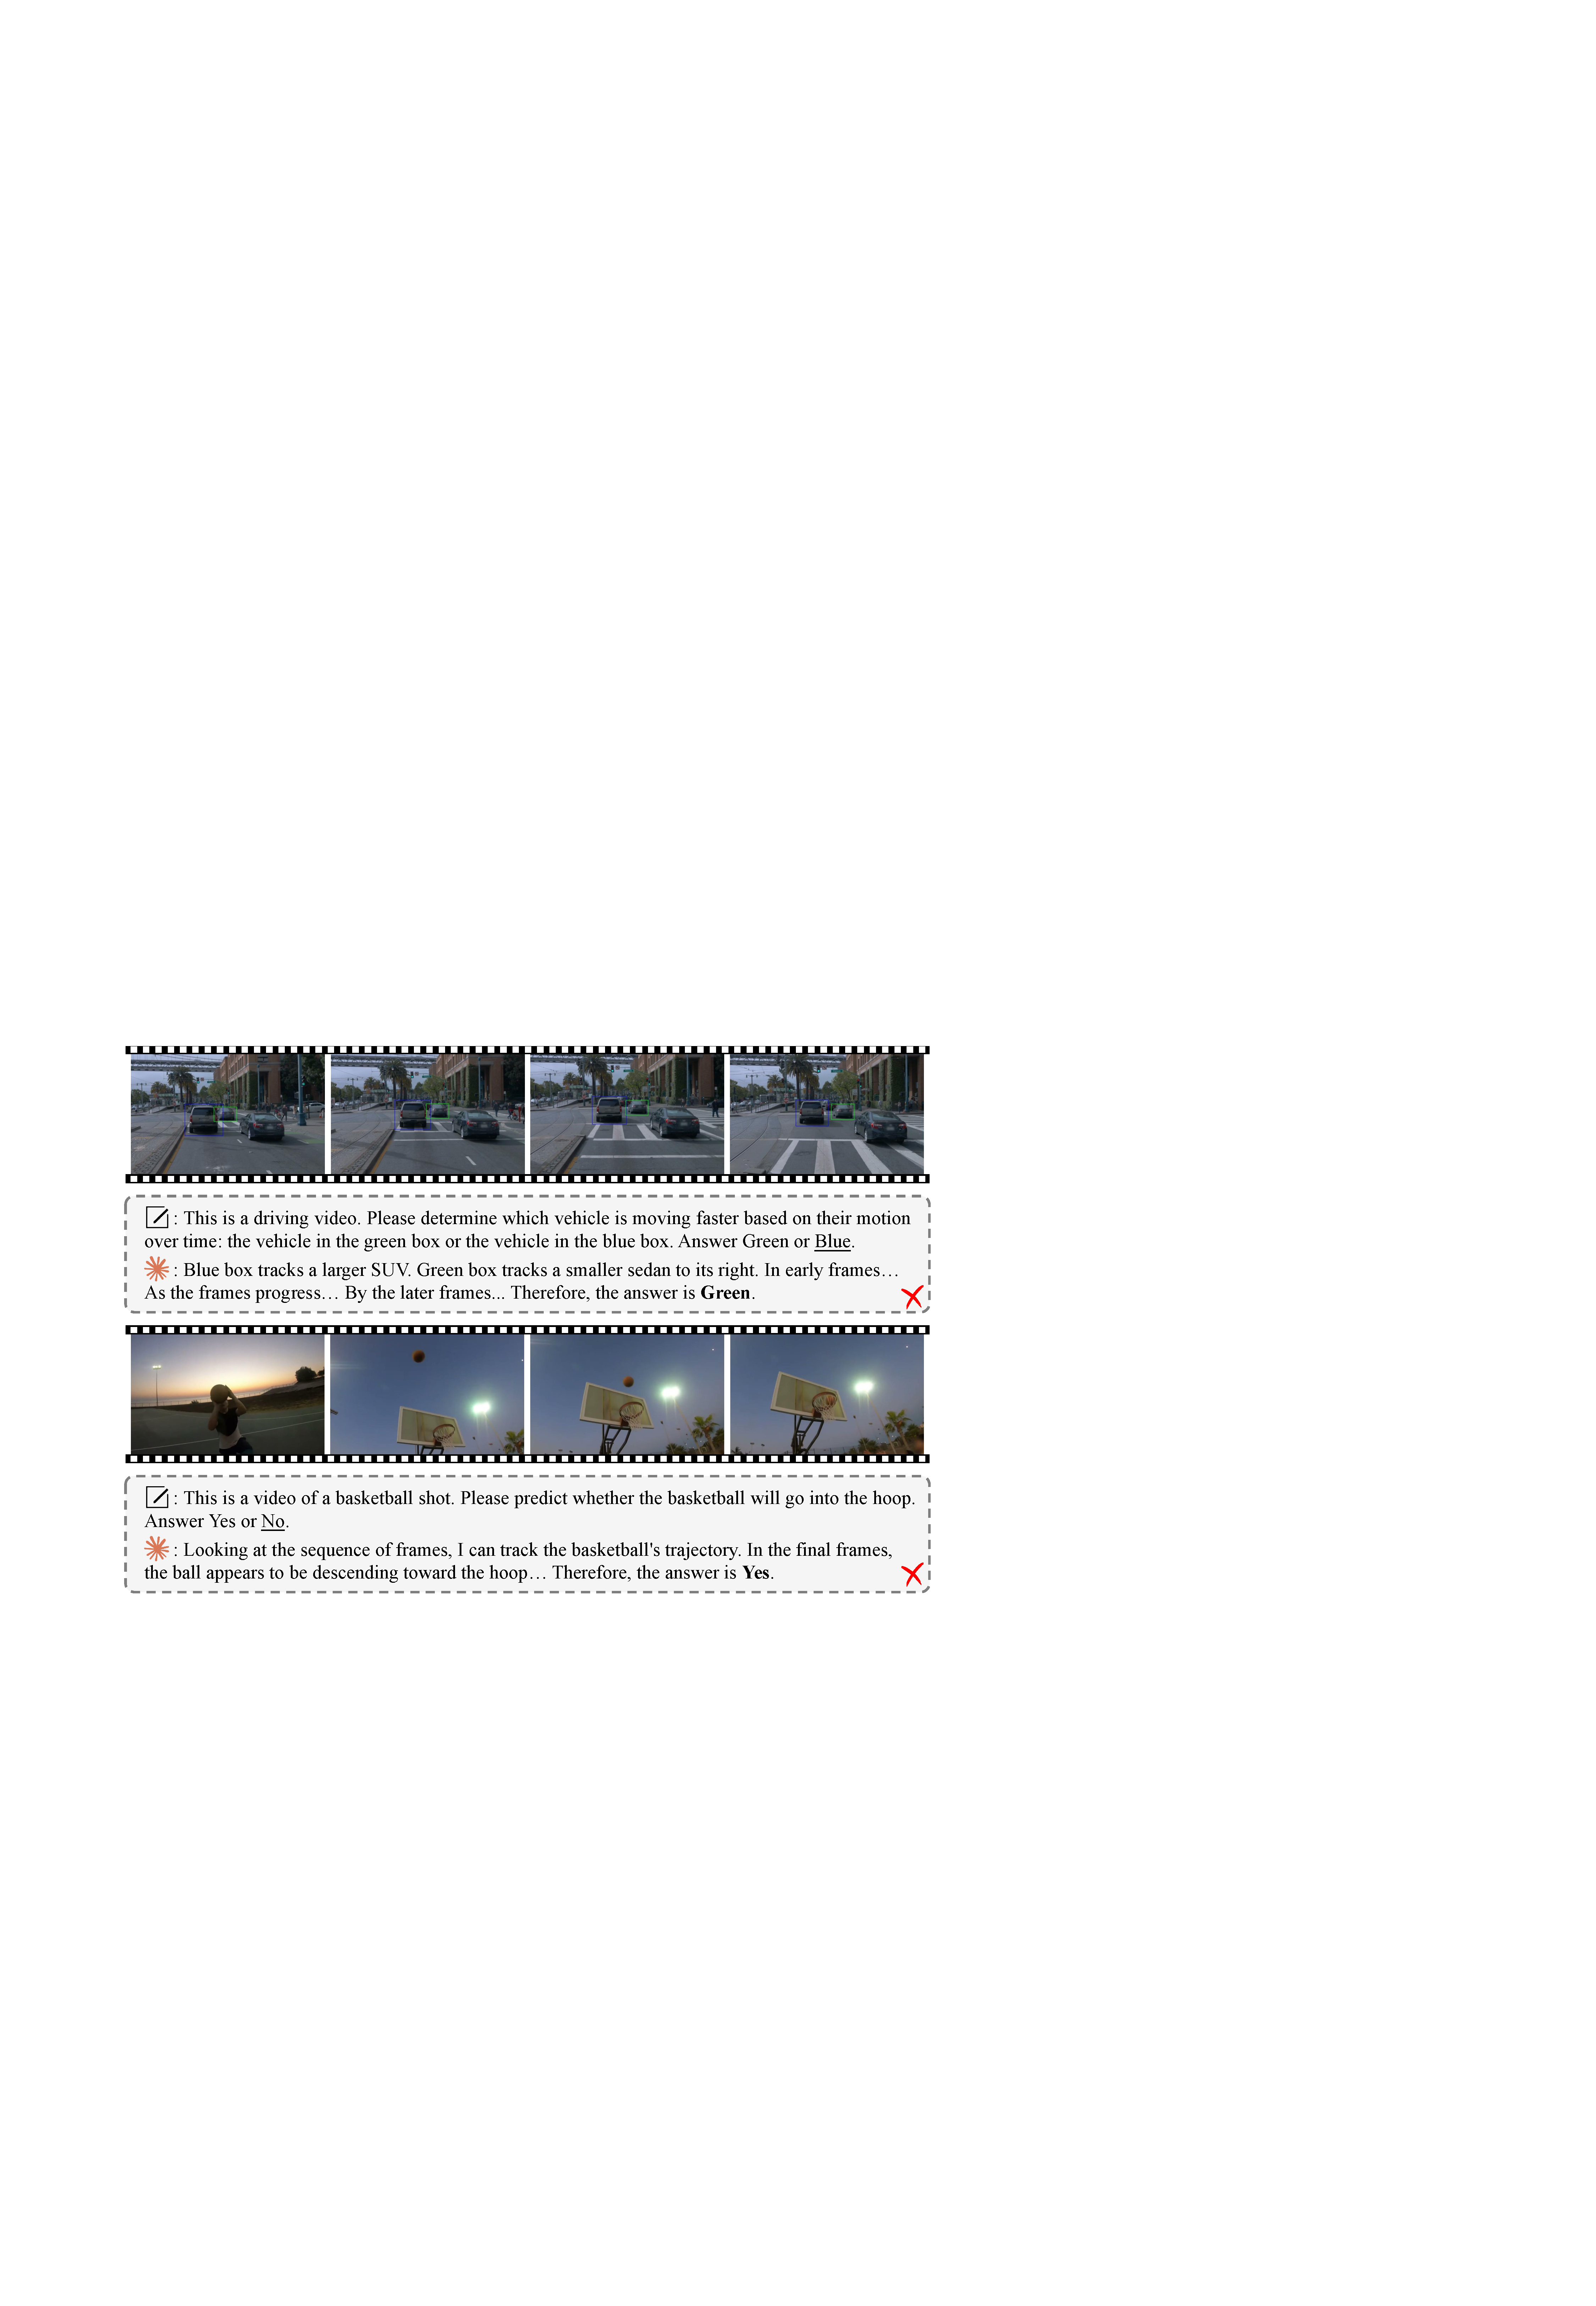
\includegraphics[height=0.25\textheight]{fig/fig_1_a.pdf}
    \caption{}
    \label{fig:1a}
  \end{subfigure}
  \begin{subfigure}{0.35\linewidth}
    \centering
    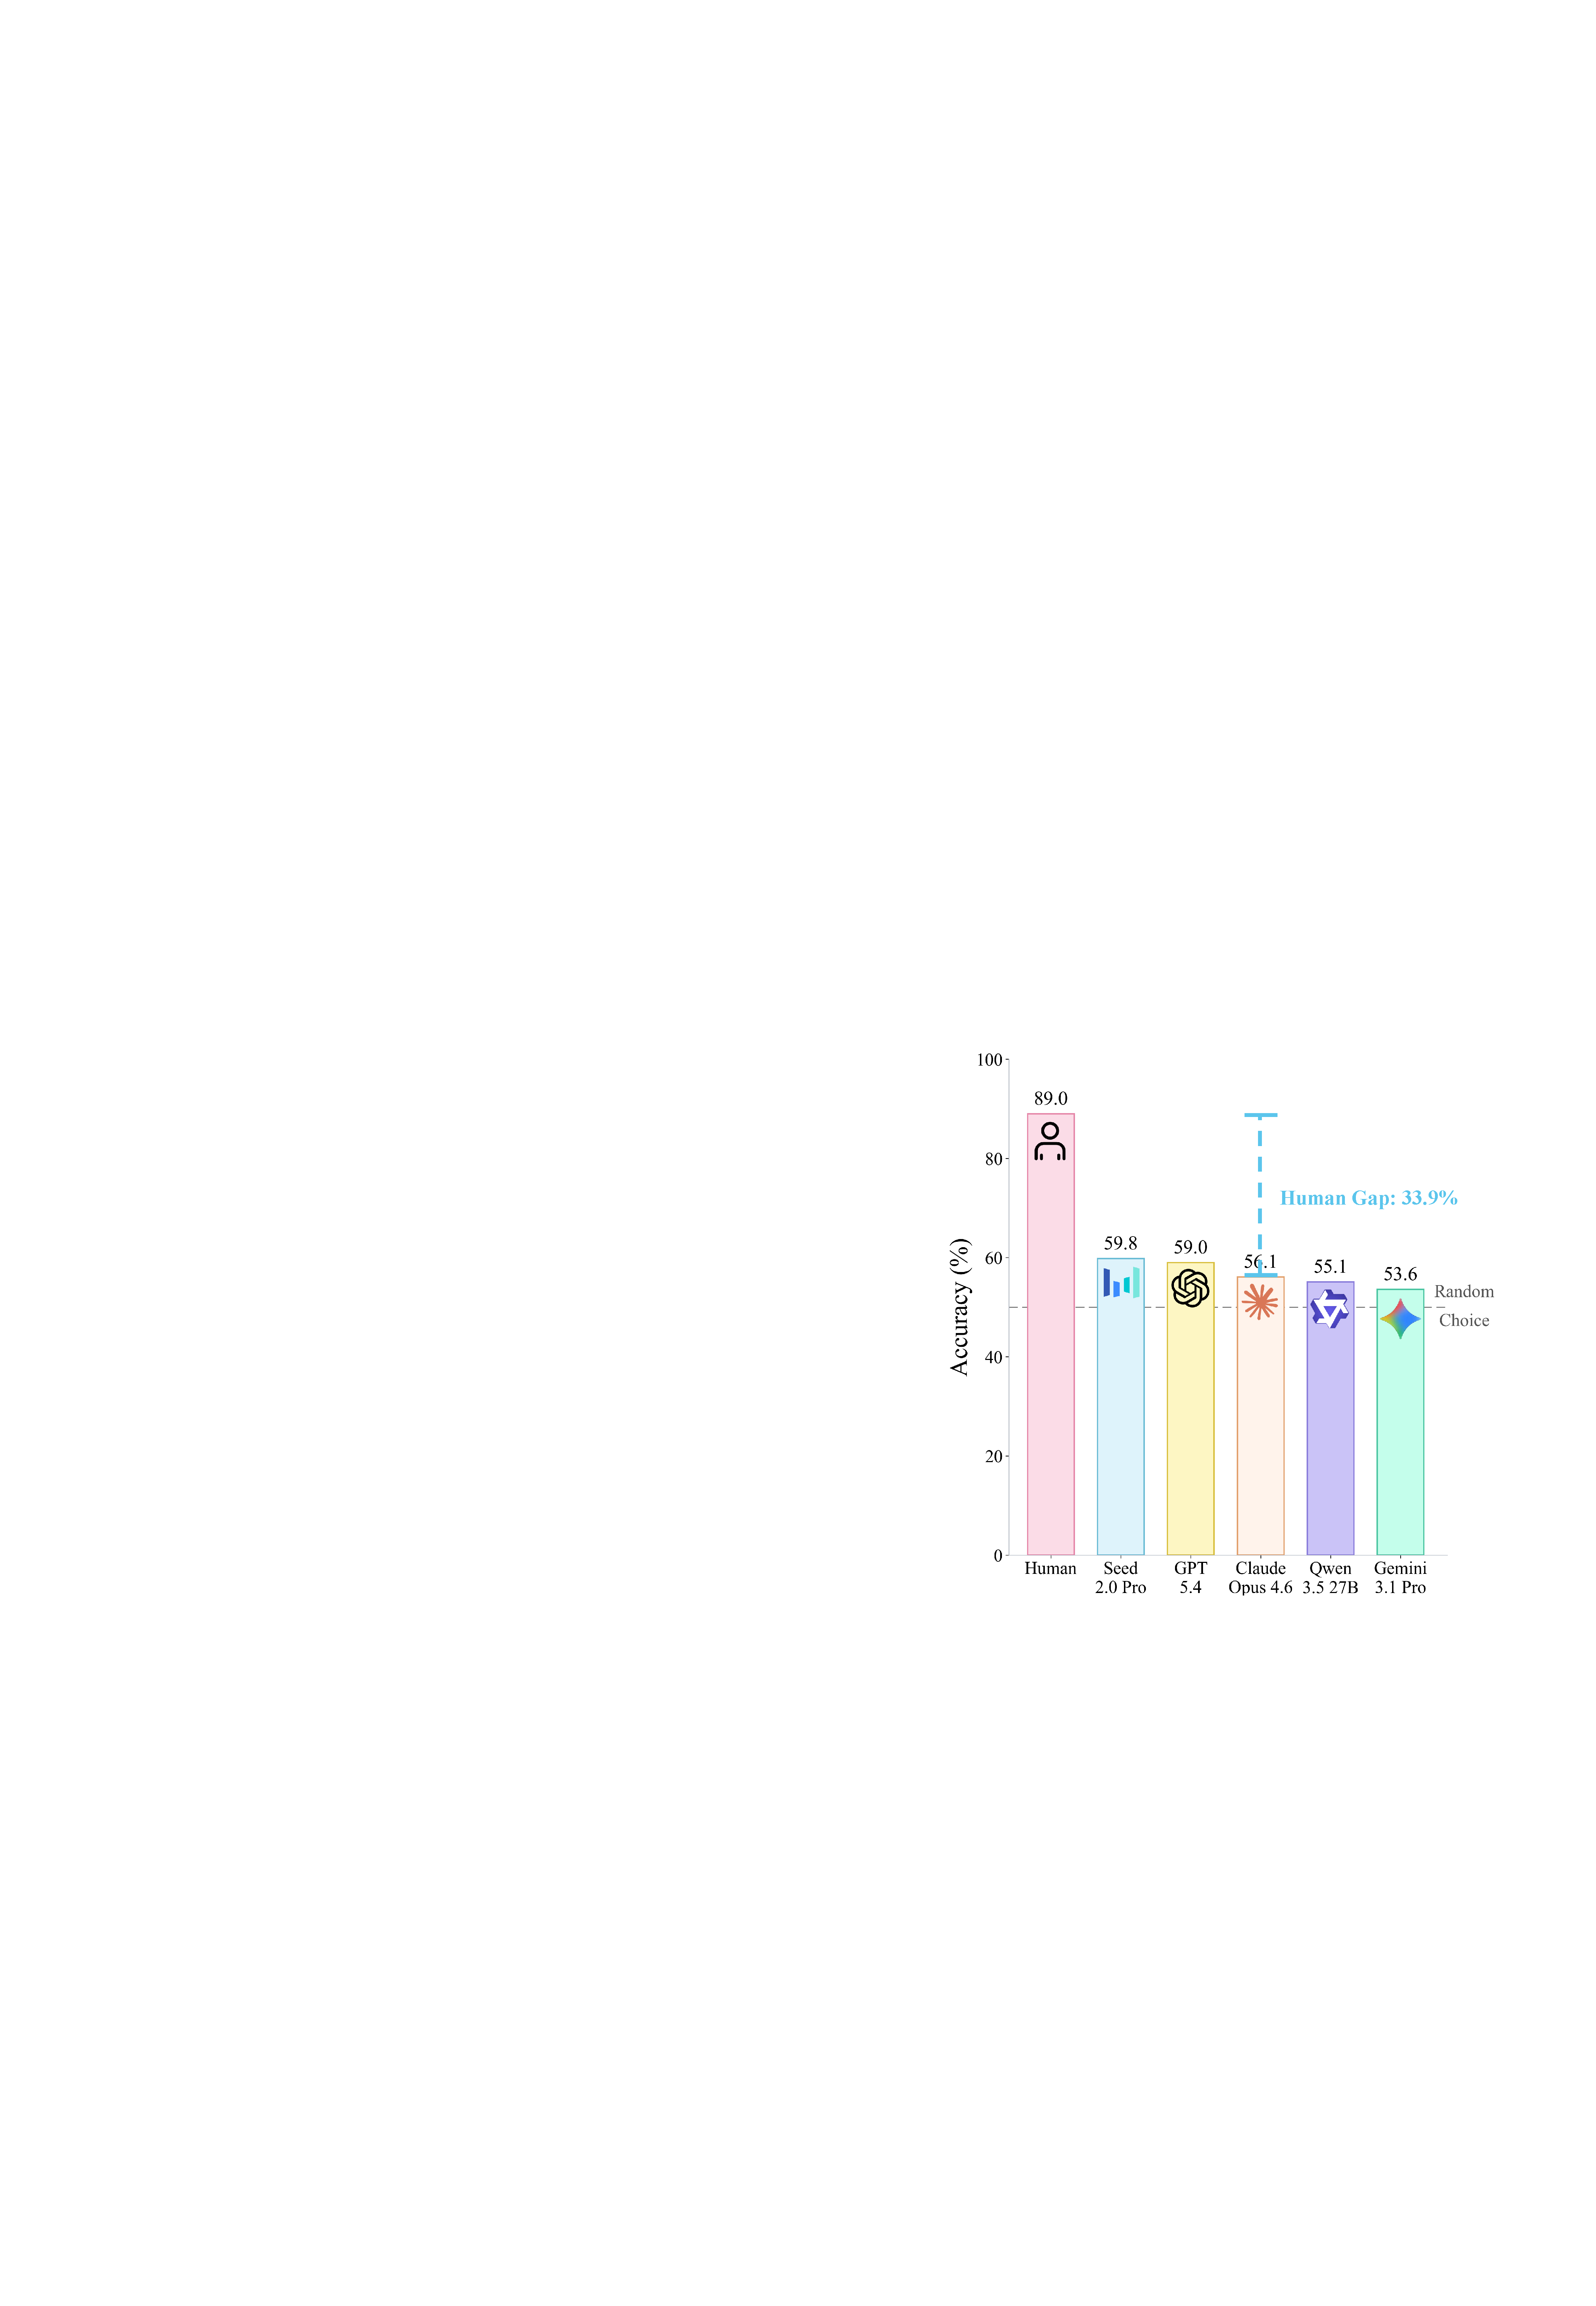
\includegraphics[height=0.25\textheight]{fig/fig_1_b.pdf}
    \caption{}
    \label{fig:1b}
  \end{subfigure}
  \caption{\textbf{Motivating examples and benchmark results.} (a) Two representative examples from ViSTR-Bench, where underlined options indicate the correct answers. Although these questions are visually straightforward for humans, Claude~\citep{Claude} still produces incorrect answers, highlighting the difficulty of reasoning from continuous visual cues in dynamic scenes. (b) Quantitative evaluation results on ViSTR-Bench, showing that current MLLMs remain far from human-level spatial-temporal reasoning performance.}
  \label{fig:1}
\end{figure}

% In recent years, Multimodal Large Language Models (MLLMs) have demonstrated remarkable proficiency across diverse domains, ranging from complex analytical tasks such as mathematical reasoning~\citep{MathVista,MATH-Vision,MATHVERSE} and programming~\citep{MMCode,Design2Code} to high-quality visual content generation~\citep{Emu3,NExT-GPT,MiniGPT-5}. 
% However, a significant gap remains between these capabilities and the physical intelligence required to reason about the real world. MLLMs still struggle with fundamental abilities that humans naturally acquire through continuous observation and interaction with the environment, including spatial perception, temporal awareness, and dynamic reasoning. 
% Such spatial-temporal reasoning capabilities are indispensable for real-world applications, including autonomous driving~\citep{LMDrive,DriveLM,DriveGPT4}, robotics~\citep{OpenVLA,RT-2}, and embodied AI~\citep{SayCan,PaLM-E}.

In recent years, Multimodal Large Language Models (MLLMs) have demonstrated remarkable proficiency across diverse domains, ranging from complex analytical tasks such as mathematical reasoning~\citep{MathVista,MATH-Vision,MATHVERSE} and programming~\citep{MMCode,Design2Code} to high-quality visual content generation~\citep{Emu3,NExT-GPT,MiniGPT-5}. 
For example, GPT-5 Pro~\citep{GPT-5} achieved 88.4\% accuracy on GPQA~\citep{GPQA}, a PhD-level scientific reasoning benchmark on which human experts achieve only 65.0\% accuracy.
However, despite these expert-level capabilities, which typically require long-term specialized training for humans to acquire, MLLMs still struggle with fundamental abilities that humans naturally develop through continuous observation and interaction with the environment, including spatial perception, temporal awareness, and dynamic reasoning, as illustrated in Figure~\ref{fig:1a}.
These spatial-temporal reasoning capabilities are indispensable for real-world applications such as autonomous driving~\citep{LMDrive,DriveLM,DriveGPT4}, robotics~\citep{OpenVLA,RT-2}, and embodied AI~\citep{SayCan,PaLM-E}.

While recent efforts have recognized this gap and introduced benchmarks to evaluate the visual spatial intelligence of MLLMs, several critical limitations remain in current task designs. 
First, existing evaluations~\citep{OmniSpatial,MMSI-Video-Bench,SpaceR,VSI-Bench,Cambrian-S,SPAR-Bench} predominantly focus on static spatial attributes, such as object scale and scene geometry, while largely neglecting the modeling of continuous temporal information. 
Second, although some benchmarks incorporate dynamic scenes~\citep{Dyn-Bench,STI-Bench,OST-Bench,VideoLoom,MLLM-4D,DSI-Bench,DSR-Bench,VLM4D}, their tasks are often restricted to low-level perception, such as object counting or trajectory tracking, falling short of the high-level reasoning needed to infer future states beyond immediate observations. 
Third, many tasks~\citep{STI-Bench,VideoLoom,MLLM-4D,DSR-Bench} rely on quantitative evaluation, which may conflate numerical prediction accuracy with genuine spatial-temporal reasoning ability.

To address these limitations, we introduce the \textbf{Vi}sual \textbf{S}patial-\textbf{T}emporal \textbf{R}easoning \textbf{Bench}mark (\textbf{ViSTR-Bench}), designed to systematically evaluate whether MLLMs can reason from continuous visual cues in dynamic scenes. 
Guided by three core principles, namely \textit{temporal emphasis}, \textit{reasoning orientation}, and \textit{qualitative evaluation}, ViSTR-Bench is structured around four task dimensions:
(1) \textbf{Motion Perception} evaluates whether models can identify and compare object motion over time, especially under ego-motion and environmental distractors;
(2) \textbf{Spatial Relations} requires models to reason about evolving geometric relationships and spatial constraints, such as observer-object relations under camera motion and collision-free passage feasibility;
(3) \textbf{Outcome Prediction} assesses the ability to infer current motion states from historical cues and anticipate future outcomes before they are directly observed; 
(4) \textbf{Physical Dynamics} focuses on intrinsic physical properties, dependencies, and stability conditions that are ambiguous in static images but become evident through dynamic interactions.

Specifically, ViSTR-Bench consists of 12 subtasks and 1,093 high-quality video question-answer pairs, spanning tabletop, indoor, and outdoor scenes. The data are collected from multiple sources, including public datasets (e.g., Ego4D~\citep{Ego4D}, ScanNet~\citep{ScanNet}, ScanNet++~\citep{ScanNet++}, ARKitScenes~\citep{ARKitScenes}, and Waymo~\citep{Waymo}), web videos, and self-collected recordings. 
We conduct extensive evaluations on a diverse set of advanced MLLMs, including proprietary general-purpose MLLMs (e.g., GPT~\citep{GPT-5}, Gemini~\citep{Gemini}, and Claude~\citep{Claude}), open-source general-purpose MLLMs (e.g., Qwen~\citep{Qwen3.5} and InternVL~\citep{InternVL3.5}), and specialized spatial MLLMs (e.g., Spatial-MLLM~\citep{Spatial-MLLM}, Spatial-SSRL~\citep{Spatial-SSRL}, and GeoThinker~\citep{GeoThinker}). As shown in Figure~\ref{fig:1b}, experimental results demonstrate that, despite the impressive progress of current MLLMs in general video question answering, they still exhibit substantial bottlenecks in tasks that require subtle motion perception, complex relational reasoning, and temporal cue modeling, with a considerable gap remaining compared to human performance.

Our main contributions are summarized as follows:
\begin{itemize}
\item We introduce the \textbf{Vi}sual \textbf{S}patial-\textbf{T}emporal \textbf{R}easoning \textbf{Bench}mark (\textbf{ViSTR-Bench}) to systematically evaluate whether MLLMs can perform qualitative spatial-temporal reasoning from continuous visual cues in dynamic scenes.

\item We establish a four-dimensional evaluation framework covering Motion Perception, Spatial Relations, Outcome Prediction, and Physical Dynamics, and construct a benchmark comprising 12 diverse subtasks and 1,093 high-quality video question-answer pairs across tabletop, indoor, and outdoor scenarios.

\item We conduct comprehensive evaluations on a broad range of advanced MLLMs, revealing that current models, despite their progress in general video question answering, still fall substantially short of human performance when understanding dynamic physical scenes.
\end{itemize}


%% ============================================================
%%  2. Related Work
%% ============================================================

\section{Related Work}
\subsection{Video Benchmarks for MLLMs}
Following the success of MLLMs in static image tasks~\citep{SEED-Bench,MMBench,MM-Vet,MMMU}, numerous benchmarks have emerged to evaluate their video understanding capabilities~\citep{MMBench-Video,Video-MME,MVBench,VITATECS,MSQA,TempCompass,OpenEQA,EgoSchema,Video-Bench,TOMATO,SpatialEval,MM-Ego}. 
However, most of them treat videos merely as temporal sequences of 2D images, leaving reasoning within 3D dynamic scenes largely underexplored. 
To address this, recent studies have evaluated the spatial intelligence of MLLMs~\citep{OmniSpatial,MMSI-Video-Bench,SpaceR,VSI-Bench,Cambrian-S,SPAR-Bench}, though they primarily focus on static properties like object size and relative positioning. 
Subsequent spatio-temporal benchmarks~\citep{Dyn-Bench,STI-Bench,OST-Bench,VideoLoom,MLLM-4D,DSI-Bench,DSR-Bench,VLM4D} introduce dynamic evaluations, such as trajectory tracking and speed estimation. 
Despite these advances, existing benchmarks predominantly assess low-level perception rather than high-level reasoning, and their reliance on quantitative predictions often conflates numerical precision with genuine spatio-temporal reasoning capabilities.

\subsection{MLLMs with Spatial Intelligence}
While MLLMs exhibit remarkable visual understanding capabilities~\citep{LLaVA-OneVision-1.5,Claude,LongVILA,LLaVA-OneVision,VILA,GPT-5,Gemini,InternVL3.5,LongVA,LLaVA-Video}, physically grounding them in the 3D world remains challenging. 
This gap has motivated a growing body of work on spatial MLLMs~\citep{SpatialVLM,VLM-3R,3DRS,GeoThinker,SpatialLadder,SpatialCoT,Spatial-SSRL,SpaceR,SoFar,Spatial-MLLM,VST,GeoSR,Think3D,VG-LLM,LLaVA-3D}.
Spatial-MLLM~\citep{Spatial-MLLM} utilizes a spatial encoder initialized with geometric priors to capture 3D structural information. 
Spatial-SSRL~\citep{Spatial-SSRL} proposes a novel self-supervised reinforcement learning paradigm aimed at enhancing LVLM spatial understanding.
Nevertheless, these approaches are largely restricted to static or indoor environments and lack the capacity to explicitly model dynamic scene evolution. 
To overcome this limitation, recent efforts have extended spatial MLLMs toward 4D reasoning for dynamic real-world settings~\citep{LLaVA-4D,Uni4D-LLM}. 
For instance, LLaVA-4D~\citep{LLaVA-4D} integrates 3D spatial coordinates and temporal cues into a unified spatio-temporal prompt, thereby facilitating comprehensive dynamic scene understanding.


%% ============================================================
%%  3. Method
%% ============================================================

\section{ViSTR-Bench}

\begin{figure}[!t]
  \centering
  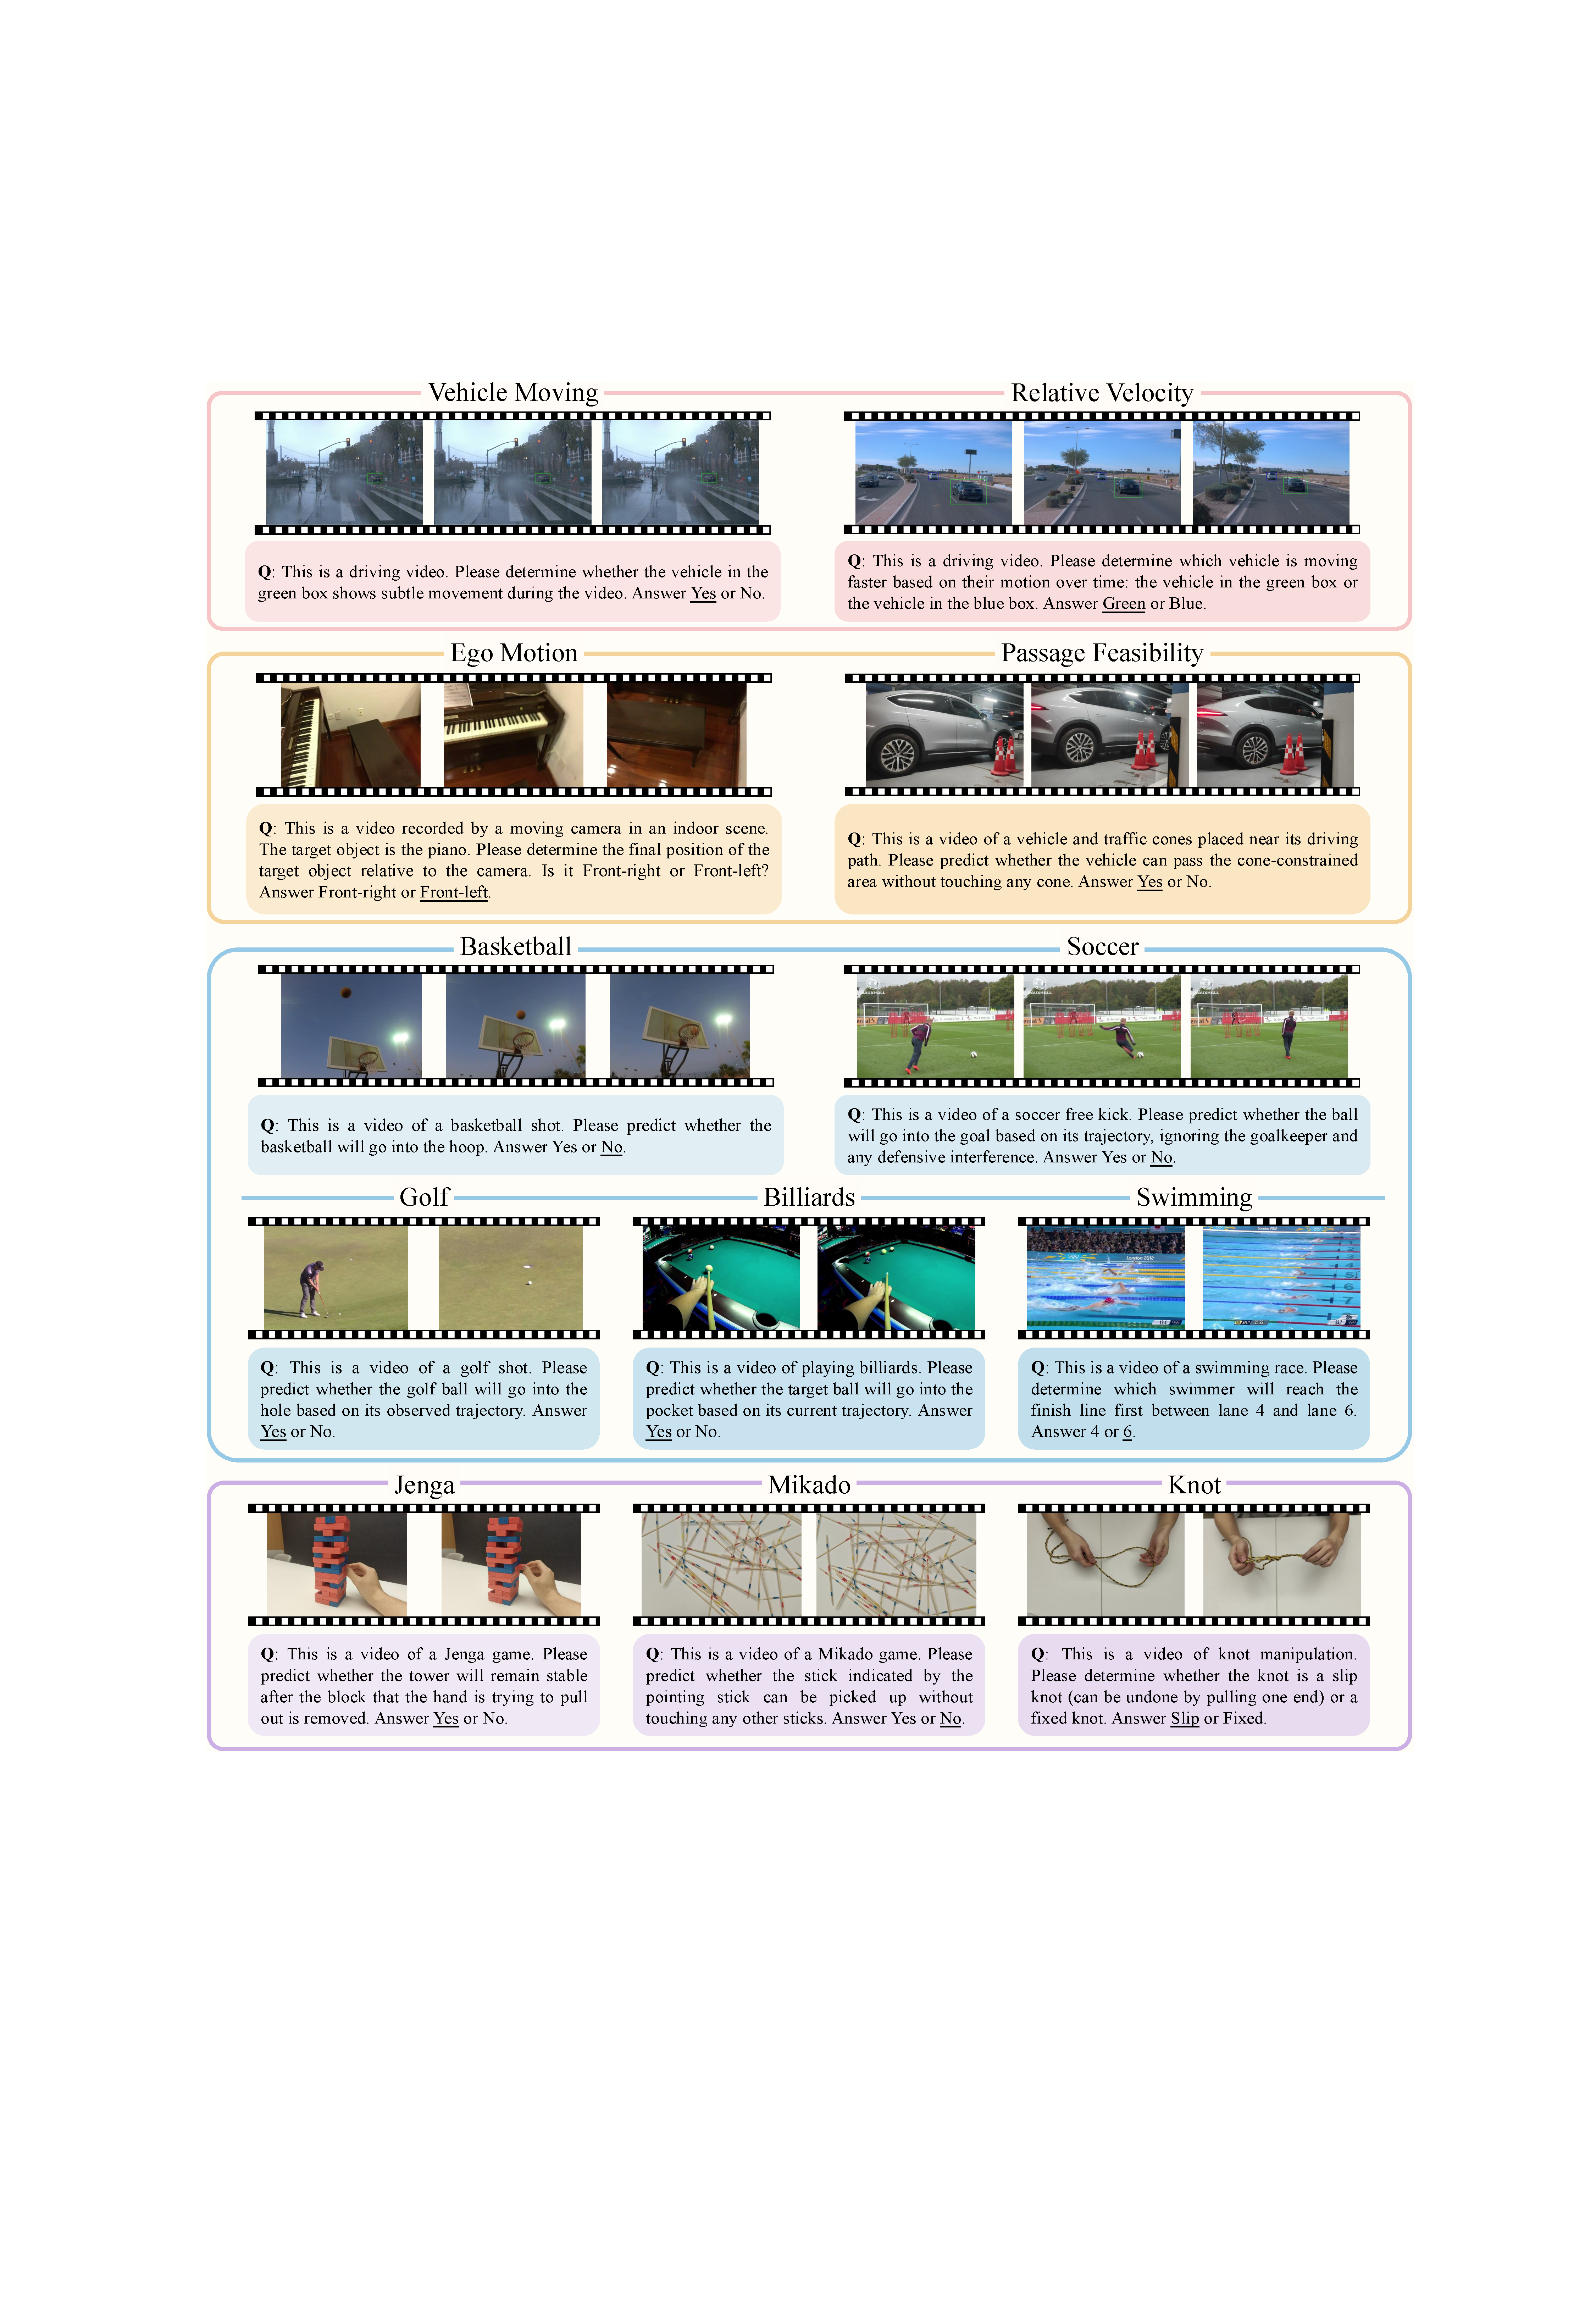
\includegraphics[height=0.70\textheight,keepaspectratio]{fig/fig_2.pdf}
  \caption{\textbf{Representative task examples from ViSTR-Bench.} Underlined options indicate the correct answers. Each task is formulated as a qualitative binary-choice question that requires models to aggregate temporal evidence and reason about dynamic visual scenes.}
  \label{fig:2}
\end{figure}

In this section, we first define the task taxonomy and reasoning objectives of ViSTR-Bench in Sec.~\ref{sec:task_definition}, and then describe the benchmark construction pipeline in Sec.~\ref{sec:benchmark_construction}.

\subsection{Task Definition}
\label{sec:task_definition}

ViSTR-Bench evaluates whether MLLMs can reason from continuous visual cues in dynamic scenes. Each task requires models to aggregate temporal evidence and make qualitative judgments about motion states, spatial relations, future outcomes, or latent physical properties. 
We organize ViSTR-Bench into four complementary dimensions, namely Motion Perception, Spatial Relations, Outcome Prediction, and Physical Dynamics, which comprise 12 subtasks in total. Representative task examples are shown in Figure~\ref{fig:2}, and the benchmark statistics are summarized in Figure~\ref{fig:3}.

\textbf{Motion Perception.}
This dimension evaluates whether MLLMs can perceive and compare object motion from continuous visual observations.
The core challenge is to distinguish true object motion from apparent visual changes caused by camera movement, viewpoint variation, or environmental distractors. 
\textit{Vehicle Movement} asks models to determine whether a target vehicle is actually moving over time. 
\textit{Relative Velocity} requires models to compare the speeds of two vehicles from an egocentric viewpoint. 
Both tasks test fundamental temporal perception abilities that cannot be reliably solved from a single static frame.

\textbf{Spatial Relations.}
This dimension focuses on reasoning about evolving spatial relationships and geometric constraints in dynamic scenes.
Unlike static spatial understanding, these tasks require models to account for camera motion, object positions, scene layout, and spatial clearance over time. 
\textit{Ego Motion} asks models to infer the spatial relationship between the observing camera and surrounding objects as the camera moves. 
\textit{Passage Feasibility} requires models to determine whether a vehicle can pass through a constrained passage without colliding with obstacles. 
These tasks emphasize observer-centric spatial reasoning and constraint-aware scene understanding.

\textbf{Outcome Prediction.}
This dimension evaluates whether MLLMs can infer future outcomes from historical motion cues before the final outcomes are directly observed. 
\textit{Basketball Shot}, \textit{Soccer Shot}, \textit{Golf Shot}, and \textit{Billiards Shot} require models to predict whether a moving object will reach a target based on its observed trajectory. 
\textit{Swimming Race} asks models to determine which swimmer will reach the finish line first from partial observations. 
These tasks require models to estimate motion trends, extrapolate trajectories, and reason about outcome-level consequences from temporal evidence.

\textbf{Physical Dynamics.}
This dimension examines whether MLLMs can reason about latent physical properties, dependencies, and stability conditions revealed through dynamic interactions. 
These properties are often ambiguous in static images but can be inferred as the physical process unfolds over time. 
\textit{Jenga Stability} requires models to predict whether a tower remains stable after block removal. 
\textit{Mikado Dependency} asks models to infer whether removing a target stick will disturb other sticks due to contact or support dependencies. 
\textit{Knot Type} requires models to identify the knot structure from its formation or manipulation process. 
These tasks go beyond visible motion and require inferring hidden physical states from temporal dynamics.

\begin{figure}[!t]
  \centering
  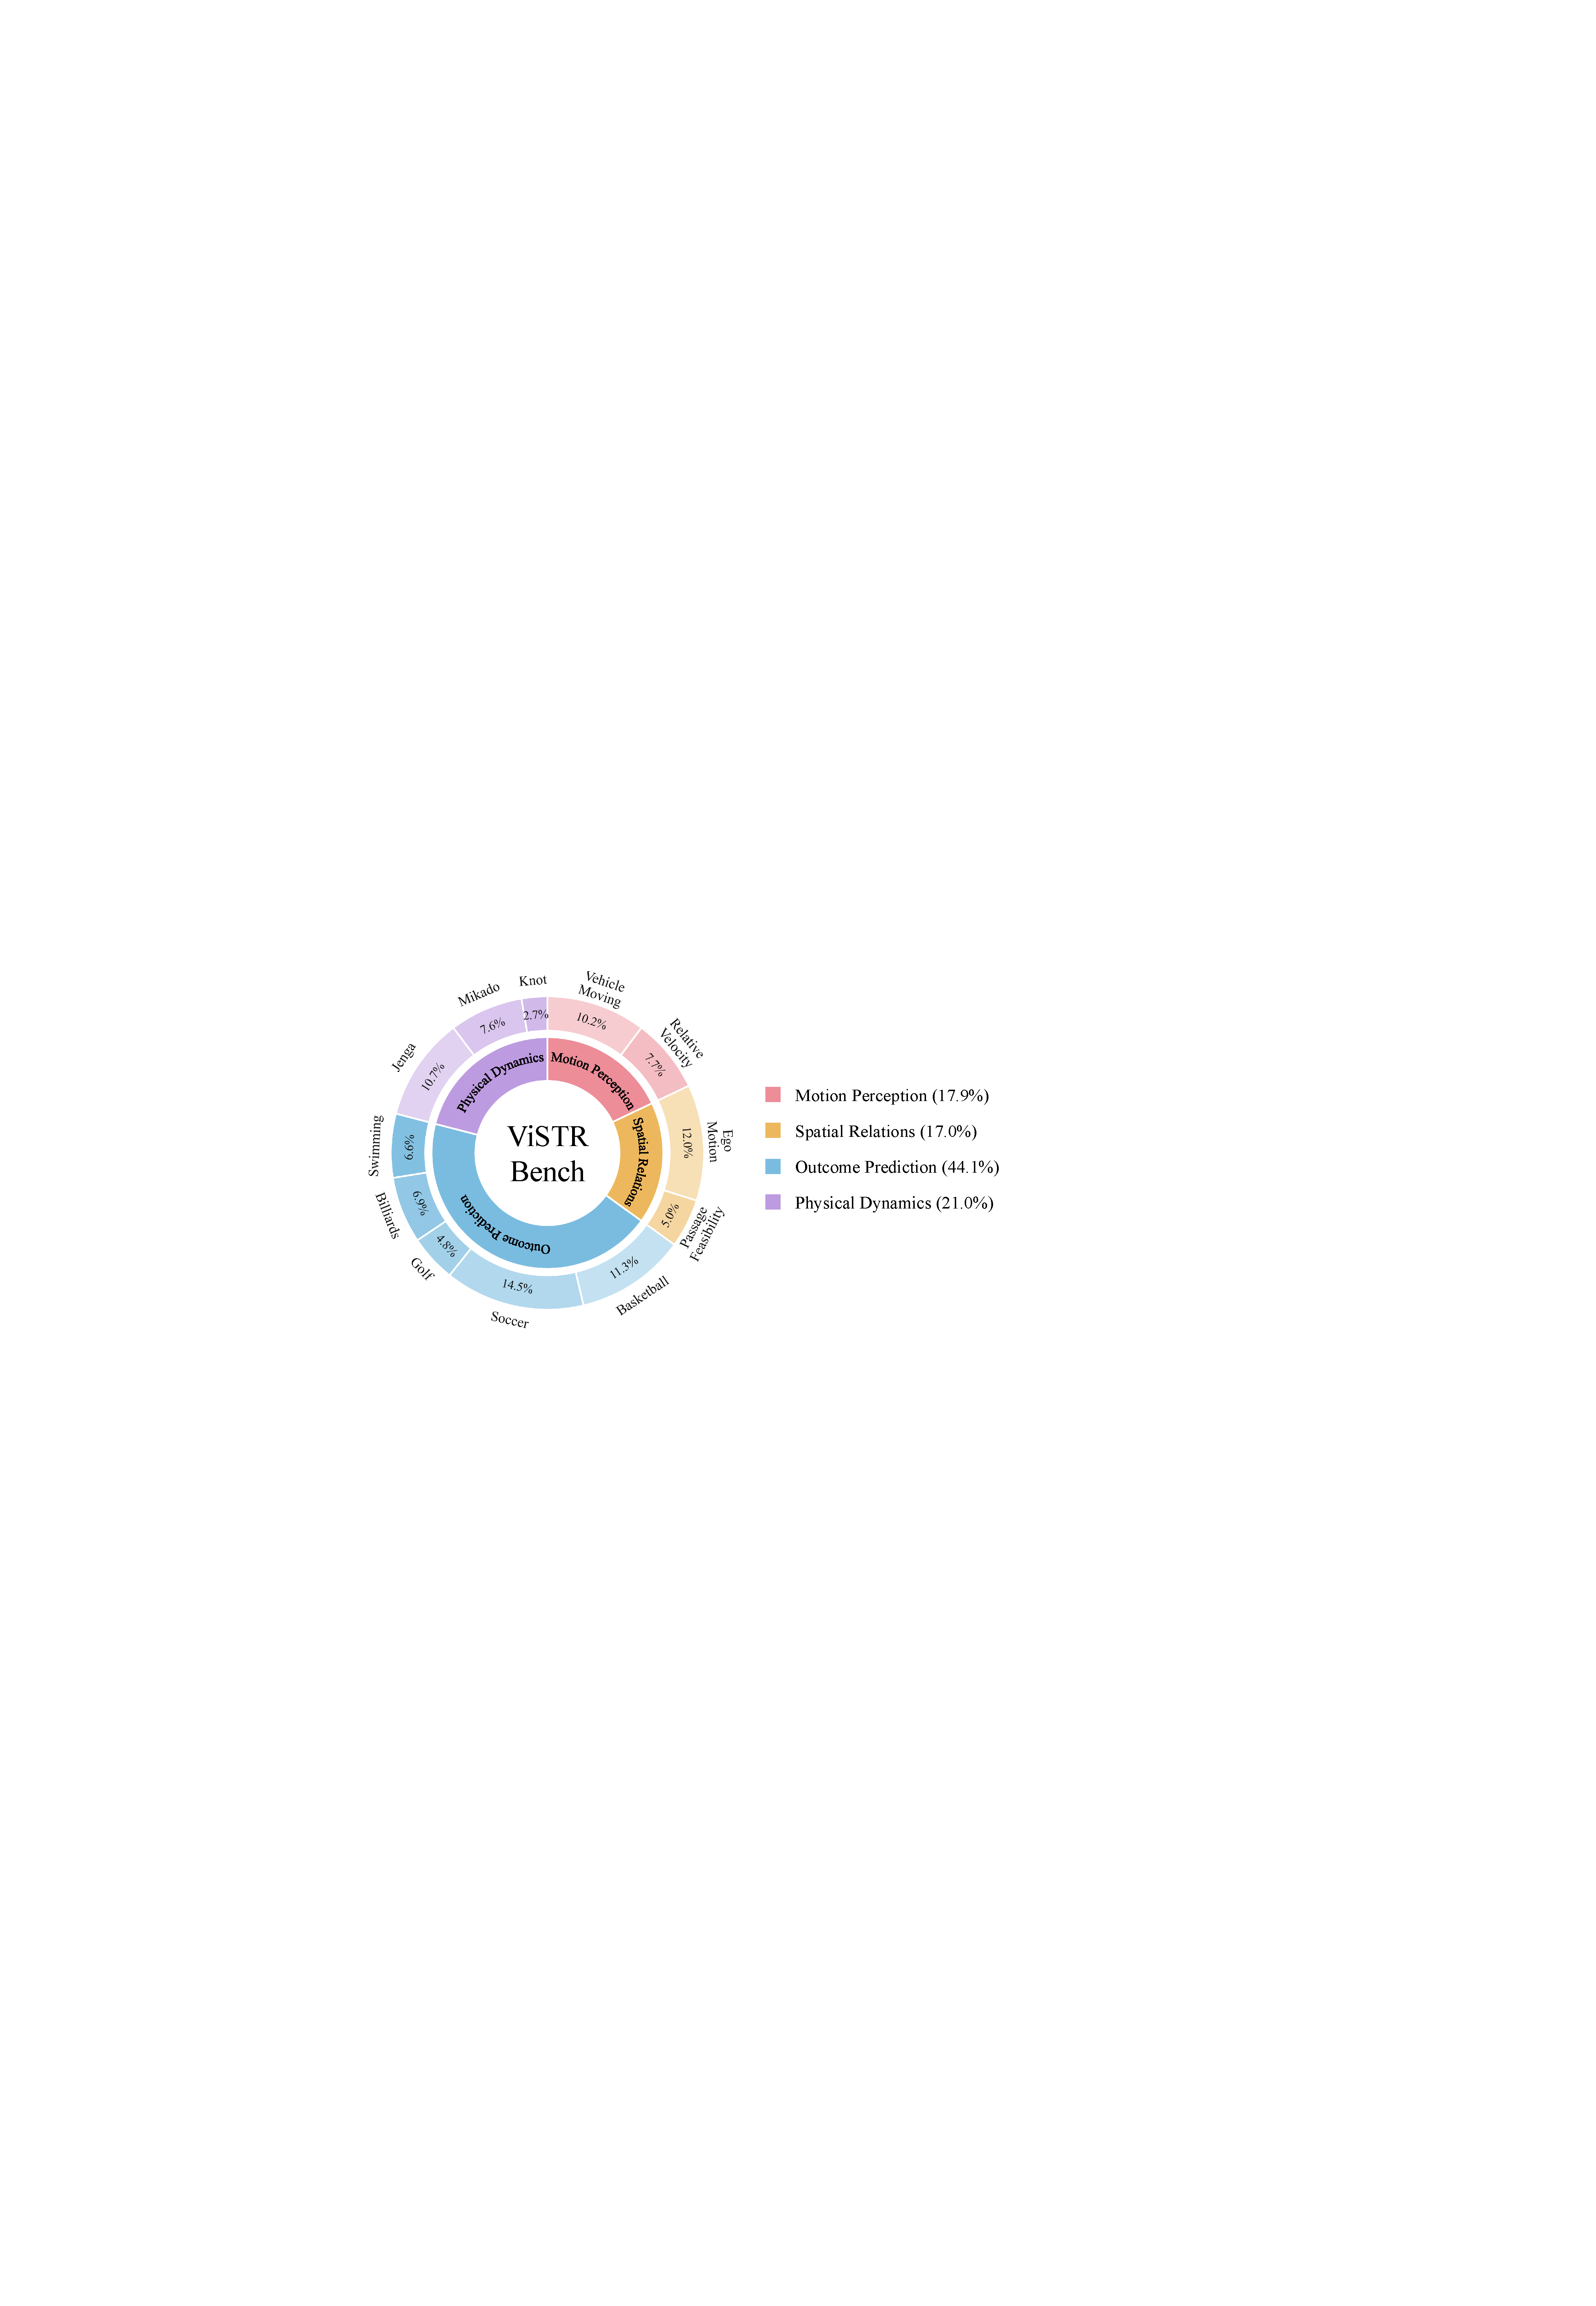
\includegraphics[width=0.60\linewidth]{fig/fig_3.pdf}
  \caption{\textbf{Benchmark statistics.} ViSTR-Bench consists of four task dimensions and 12 subtasks.}
  \label{fig:3}
\end{figure}

\subsection{Benchmark Construction}
\label{sec:benchmark_construction}

We construct ViSTR-Bench through a systematic multi-stage pipeline, including data collection, video preprocessing, question-answer (QA) pair generation, and human quality control, as shown in Figure~\ref{fig:4}. 
This pipeline is designed to ensure that each sample requires temporal evidence, supports high-level reasoning, and has an unambiguous qualitative answer.

\textbf{Data Collection.}
To cover diverse spatio-temporal reasoning scenarios across tabletop, indoor, and outdoor environments, we collect videos from established public datasets, curated web videos, and self-collected recordings.
Specifically, for autonomous driving scenarios, we sample videos from the Waymo Open Dataset~\citep{Waymo}. 
For indoor spatial reasoning, we use egocentric videos from ScanNet~\citep{ScanNet}, ScanNet++~\citep{ScanNet++}, and ARKitScenes~\citep{ARKitScenes}. 
For sports-related outcome prediction, we extract relevant clips from Ego4D~\citep{Ego4D} and further supplement them with web videos of corresponding sporting events. 
For specialized tasks that are difficult to construct from existing datasets, such as Passage Traversability and tabletop Physical Dynamics tasks, we conduct task-specific recordings in controlled real-world environments. 
Details of data sources are provided in Appendix~\ref{sec:detailed_data_sources}. 

\textbf{Video Preprocessing.}
Raw videos inherently contain multiple distinct events, irrelevant temporal context, and explicit outcomes that could trivialize reasoning tasks into simple recognition. 
To systematically eliminate these confounding factors and prevent shortcut learning by models, we process all collected videos through a three-stage preprocessing pipeline:
(1) \textbf{Event Localization.} 
To prevent the entanglement of multiple events and isolate specific reasoning instances, we localize raw videos into discrete, event-level clips and strip away unrelated temporal context.
(2) \textbf{Visual Prompting.} 
For object-centric tasks, textual descriptions alone may introduce referential ambiguity, especially in cluttered scenes with multiple similar objects. 
To explicitly ground target objects, we overlay visual markers (e.g., bounding boxes) onto the corresponding video frames. 
For instance, in the Vehicle Movement and Relative Velocity tasks, we leverage dataset annotations to highlight the specific vehicles in question.
(3) \textbf{Outcome Truncation.} 
For tasks in which the terminal outcome directly reveals the answer, we truncate videos before the outcome becomes visually explicit. 
Instead of using a fixed truncation ratio, we manually determine an instance-specific decision point for each clip, ensuring that the retained segment contains sufficient temporal evidence for human annotators to make a confident qualitative judgment. 
Collectively, these preprocessing steps standardize the visual inputs and mitigate confounding factors from irrelevant context, referential ambiguity, and answer-revealing frames.

\textbf{QA Pair Generation.}
We formulate all instances as binary-choice questions using task-specific templates. Detailed prompt templates are provided in Appendix~\ref{sec:detailed_prompt_templates}.
While most subtasks inherently follow a binary format, those with broader answer spaces, such as the Ego Motion task involving directions including front-left, front-right, back-left, and back-right, are converted to fit this framework. 
Specifically, we pair the ground-truth answer with a plausible distractor randomly sampled from the remaining valid options. To mitigate positional bias during model evaluation, the order of the two candidate options is systematically randomized for each question.

\textbf{Human Quality Control.}
To ensure the reliability of ViSTR-Bench, expert annotators manually filter all candidate QA pairs according to four strict criteria. 
Specifically, we first verify the \textit{visibility} of target objects, ensuring that they are identifiable based on either the textual description or visual prompts. 
We then examine the temporal \textit{sufficiency} of each clip to ensure that it contains adequate visual evidence for reasoning. 
Furthermore, we ensure the \textit{objectivity} of the dataset by requiring all ground-truth answers to be definitive and fully consistent with the observed visual events. 
Finally, we enforce a strict \textit{non-triviality} standard by discarding samples that can be trivially answered from a single static frame or by common-sense language priors. 
Through this rigorous review process, ViSTR-Bench establishes a reliable evaluation foundation for continuous spatio-temporal reasoning.

\begin{figure}[!t]
  \centering
  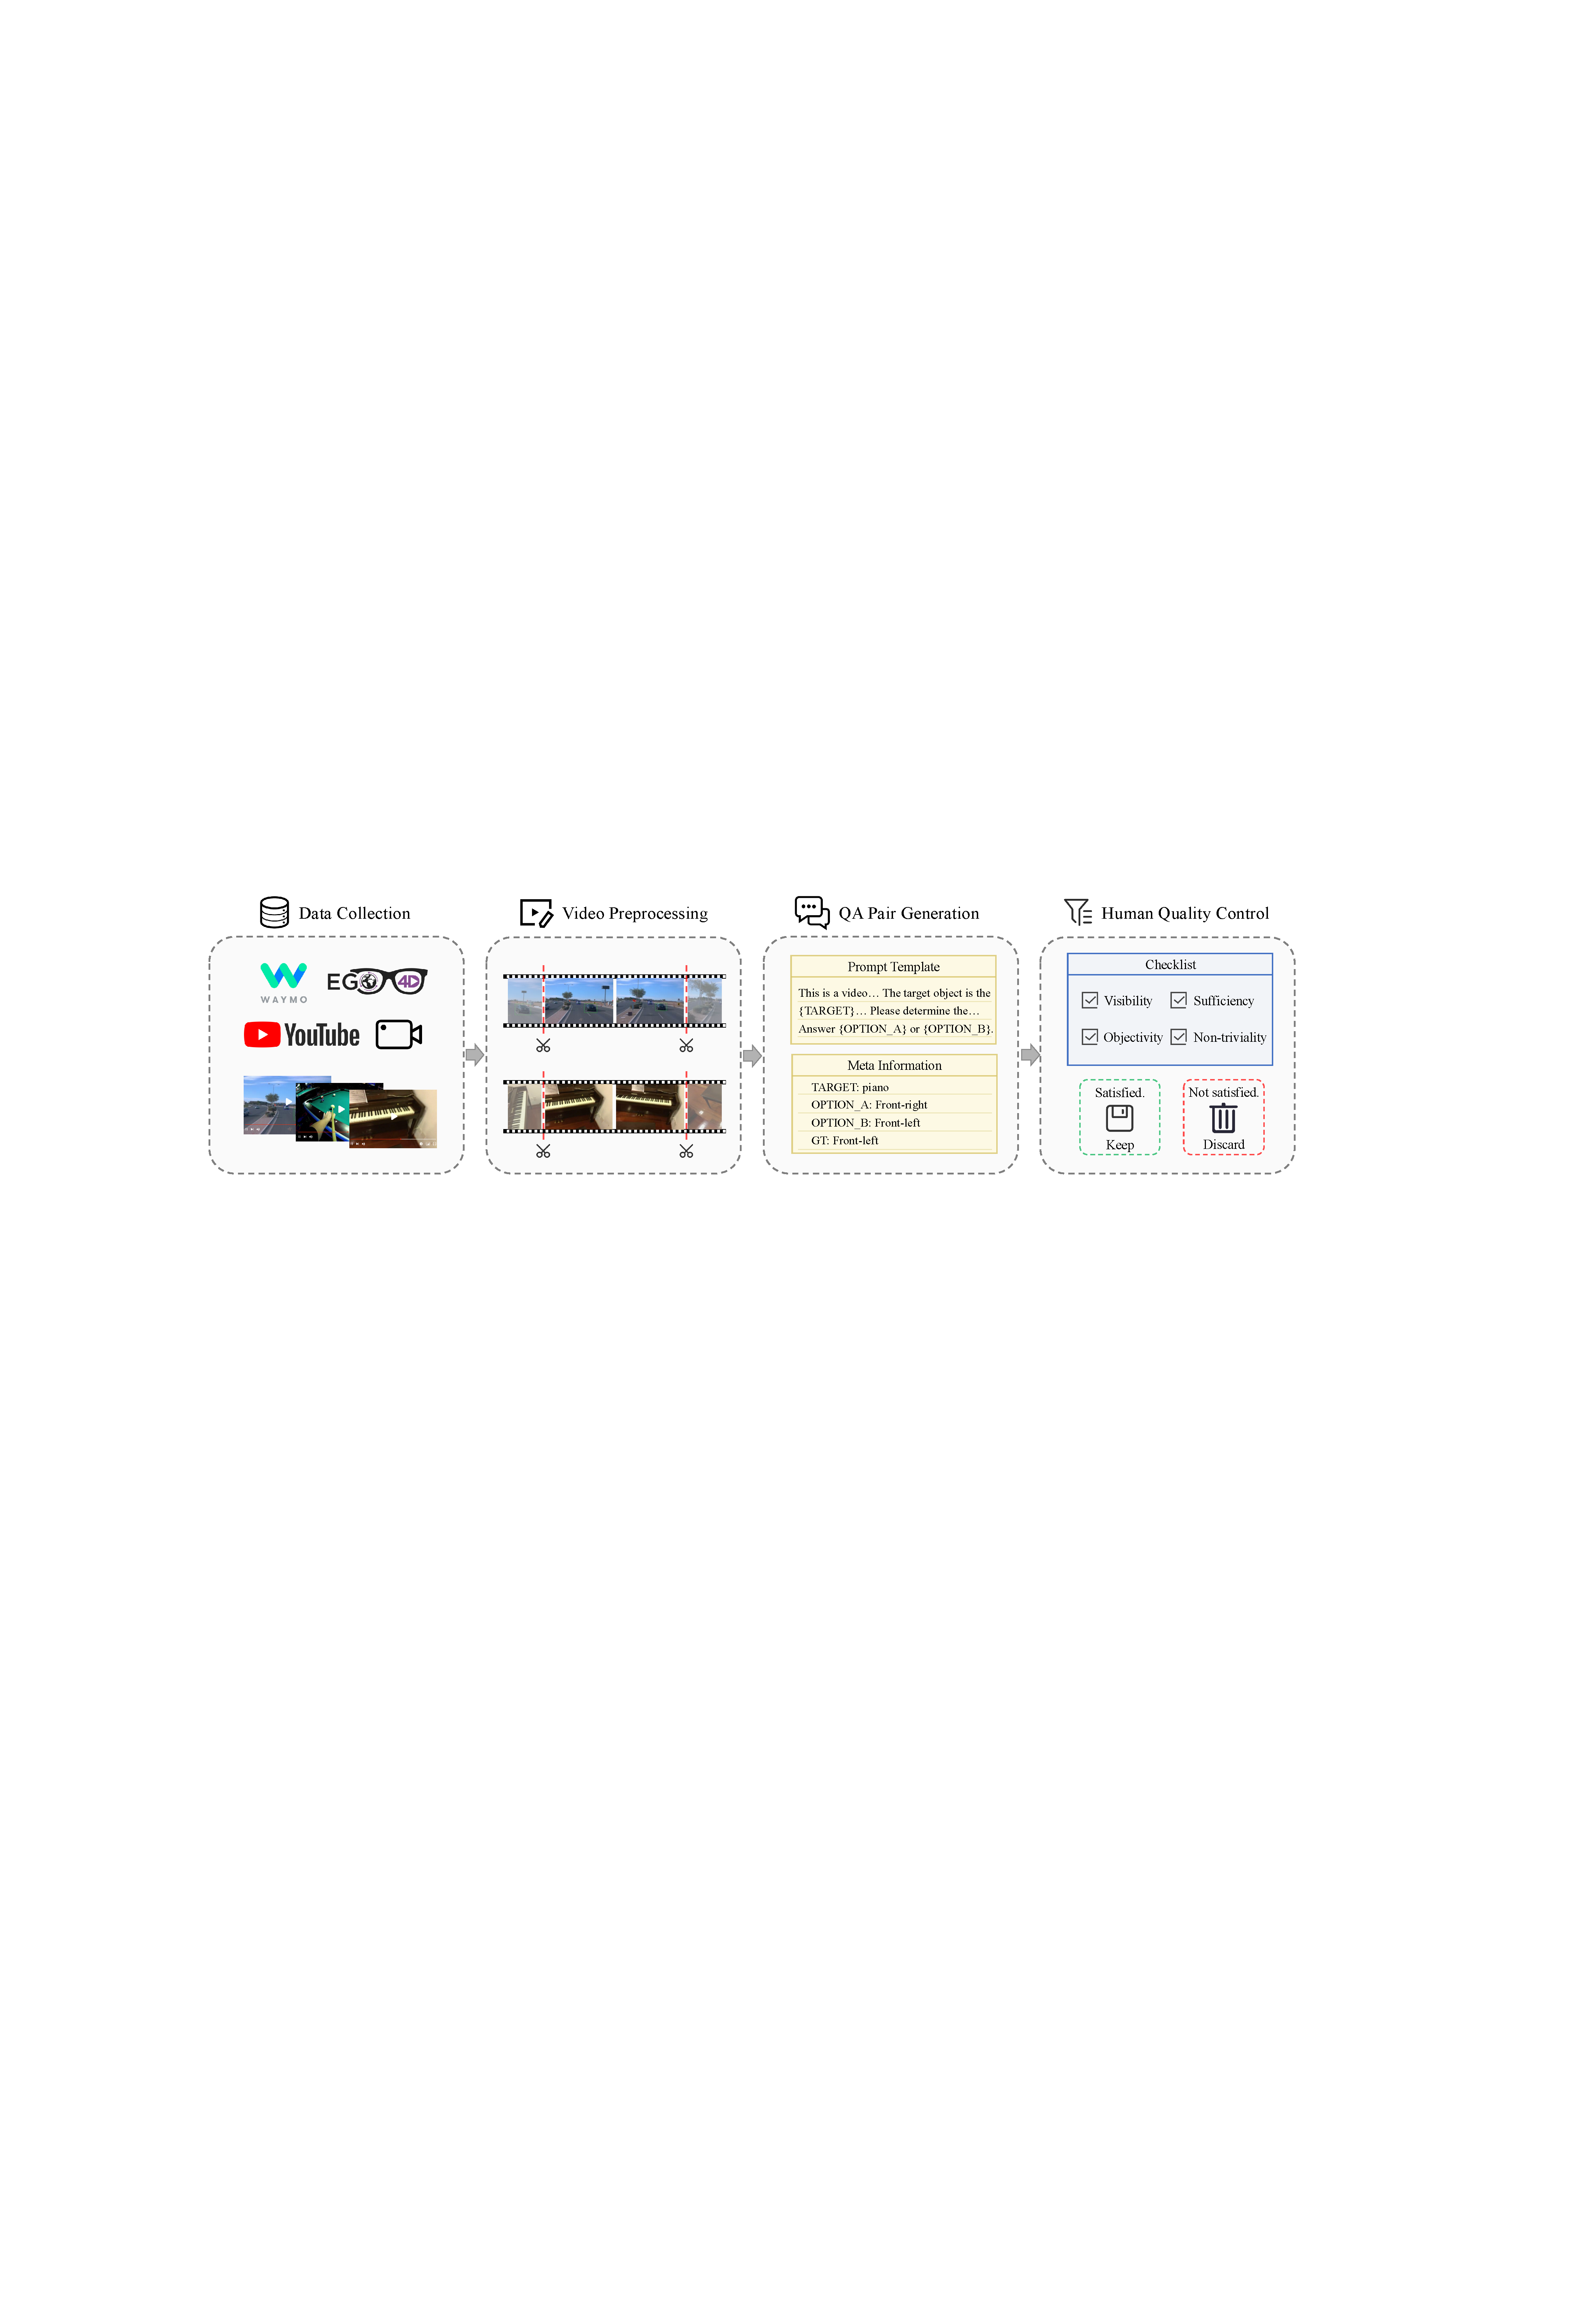
\includegraphics[width=0.95\linewidth]{fig/fig_4.pdf}
  \caption{\textbf{Benchmark construction pipeline.} We construct ViSTR-Bench through a systematic multi-stage process, including data collection, video preprocessing, QA pair generation, and human quality control. This pipeline ensures that each sample contains sufficient temporal evidence, supports high-level reasoning, and has an unambiguous qualitative answer.}
  \label{fig:4}
\end{figure}


%% ============================================================
%%  4. Experiments
%% ============================================================

\section{Evaluation on ViSTR-Bench}

\begin{table}[!t]
    \centering
    \caption{
        \textbf{Main results on ViSTR-Bench.} 
        We report accuracy (\%) across 12 subtasks grouped into four reasoning dimensions.
        The suffix \emph{-thinking} indicates that the model is evaluated with its built-in thinking mode enabled.
        \emph{Avg.} denotes the overall accuracy averaged over all question-answer pairs, and \emph{Rank} denotes the ranking within each model category.
        The best and second-best results within each model group are highlighted with \bestcap{} and \secondcap{}, respectively.
    }
    \label{tab:main_results}

    \resizebox{\textwidth}{!}{
    \begin{tabular}{l c c cc cc ccccc ccc}
        \toprule
        \multirow{2}{*}{\textbf{Method}} 
        & \multirow{2}{*}{\textbf{Rank}} 
        & \multirow{2}{*}{\textbf{Avg.}} 
        & \multicolumn{2}{c}{\textbf{Motion Perc.}} 
        & \multicolumn{2}{c}{\textbf{Spat. Rela.}} 
        & \multicolumn{5}{c}{\textbf{Outc. Pred.}}  
        & \multicolumn{3}{c}{\textbf{Phys. Dyna.}} \\
        \cmidrule(lr){4-5} \cmidrule(lr){6-7} \cmidrule(lr){8-12} \cmidrule(lr){13-15}
        & & 
        & \makecell{Vehi.\\Move.} & \makecell{Rela.\\Velo.} 
        & \makecell{Ego\\Motion} & \makecell{Pass.\\Feas.} 
        & Bask. & Soccer & Golf & Bill. & Swim.
        & Jenga & Mikado & Knot \\
        \midrule

        \rowcolor{groupbg}
        \multicolumn{15}{l}{\textbf{Baseline}} \\
        Chance Level (Random) & - & 50.0 & 50.0 & 50.0 & 50.0 & 50.0 & 50.0 & 50.0 & 50.0 & 50.0 & 50.0 & 50.0 & 50.0 & 50.0 \\
        Chance Level (Frequency) & - & 57.2 & 64.3 & 59.5 & 53.4 & 65.5 & 57.3 & 52.5 & 54.7 & 53.3 & 50.0 & 65.0 & 54.2 & 58.6 \\
        \midrule

        \rowcolor{groupbg}
        \multicolumn{15}{l}{\textbf{Proprietary General MLLMs}} \\
        GPT-5.4 & 9 & 54.9 & 66.1 & 67.9 & 63.4 & 67.3 & 42.7 & 53.2 & 45.3 & 52.0 & 51.4 & 46.2 & 45.8 & 69.0 \\
        GPT-5.4-thinking & 3 & 59.0 & 57.1 & \second{75.0} & \best{75.6} & 58.2 & 46.8 & 51.3 & \second{54.7} & \best{58.7} & 50.0 & \best{67.5} & 47.0 & \second{72.4} \\
        Gemini-3-Flash-Preview & 17 & 50.0 & 35.7 & 44.0 & 55.7 & 63.6 & 44.4 & 54.4 & 49.1 & 53.3 & \second{59.7} & 44.4 & 50.6 & 62.1 \\
        Gemini-3.1-Flash-Lite-Preview & 13 & 52.4 & 45.5 & 50.0 & 62.6 & 63.6 & 53.2 & 46.8 & 49.1 & 36.0 & \second{59.7} & 60.7 & 44.6 & 65.5 \\
        Gemini-3.1-Pro-Preview & 11 & 53.6 & 45.5 & 52.4 & \second{72.5} & 65.5 & \best{56.5} & 50.0 & 43.4 & 54.7 & 50.0 & 42.7 & 47.0 & \best{75.9} \\
        Claude-Sonnet-4.6 & 16 & 52.0 & \second{67.9} & 40.5 & 64.9 & 52.7 & 54.8 & 55.1 & 50.9 & 48.0 & 50.0 & 34.2 & 38.6 & 62.1 \\
        Claude-Sonnet-4.6-thinking & 8 & 55.4 & 67.0 & 40.5 & 66.4 & 52.7 & 51.6 & \second{62.0} & \best{58.5} & 52.0 & 51.4 & 48.7 & 44.6 & 62.1 \\
        Claude-Opus-4.6 & 4 & 57.0 & 65.2 & 45.2 & 64.1 & \best{70.9} & 49.2 & \best{63.3} & 50.9 & 40.0 & 50.0 & \second{65.8} & 44.6 & \second{72.4} \\
        Claude-Opus-4.6-thinking & 6 & 56.1 & 65.2 & 40.5 & 71.8 & 67.3 & 44.4 & 56.3 & 52.8 & 46.7 & 50.0 & 65.0 & 48.2 & 55.2 \\
        Seed-2.0-Lite & 7 & 56.0 & 64.3 & 60.7 & 51.1 & 63.6 & 52.4 & 55.7 & 49.1 & 49.3 & 48.6 & 65.0 & \second{55.4} & 48.3 \\
        Seed-2.0-Lite-thinking & \second{2} & \second{59.7} & \best{68.8} & 67.9 & 66.4 & 65.5 & 49.2 & 61.4 & \best{58.5} & 48.0 & 51.4 & 65.0 & 51.8 & 51.7 \\
        Seed-2.0-Pro & 5 & 56.6 & 57.1 & 67.9 & 58.0 & \best{70.9} & 52.4 & 51.3 & 47.2 & \best{58.7} & 55.6 & 63.2 & 48.2 & 48.3 \\
        Seed-2.0-Pro-thinking & \best{1} & \best{59.8} & 63.4 & \best{81.0} & 67.9 & \second{69.1} & \second{55.6} & 53.2 & 49.1 & 54.7 & \best{66.7} & 57.3 & 45.8 & 51.7 \\
        MiMo-V2-Omni & 14 & 52.1 & 64.3 & 51.2 & 58.8 & 58.2 & 45.2 & 43.7 & 41.5 & 52.0 & 43.1 & 63.2 & 44.6 & 58.6 \\
        MiMo-V2-Omni-thinking & 10 & 54.1 & 55.4 & 45.2 & 63.4 & \best{70.9} & 44.4 & 55.1 & 43.4 & 49.3 & 48.6 & 58.1 & \best{56.6} & 58.6 \\
        MiMo-V2.5 & 15 & 52.0 & 59.8 & 40.5 & 64.9 & 50.9 & 42.7 & 55.7 & 37.7 & \second{56.0} & 52.8 & 51.3 & 42.2 & 62.1 \\
        MiMo-V2.5-thinking & 12 & 52.5 & 51.8 & 38.1 & 58.0 & 63.6 & 50.8 & 53.8 & 35.8 & 50.7 & 51.4 & 60.7 & 53.0 & 55.2 \\
        \midrule

        \rowcolor{groupbg}
        \multicolumn{15}{l}{\textbf{Open-source General MLLMs}} \\
        LLaVA-OneVision-1.5-4B & 14 & 47.8 & 60.7 & 36.9 & 52.7 & 65.5 & 42.7 & 47.5 & 54.7 & 46.7 & 50.0 & 35.0 & 45.8 & 41.4 \\
        LLaVA-OneVision-1.5-8B & 11 & 48.9 & \second{63.4} & 40.5 & 53.4 & 65.5 & 41.9 & 47.5 & 50.9 & 48.0 & 50.0 & 38.5 & 45.8 & 51.7 \\
        Qwen3.5-27B-thinking & \best{1} & \best{55.1} & 60.7 & 50.0 & 62.6 & 65.5 & \best{59.7} & \best{55.1} & 49.1 & 49.3 & \second{58.3} & 47.9 & 44.6 & 51.7 \\
        Qwen3.5-35B-A3B-thinking & 13 & 48.7 & 46.4 & 45.2 & 58.0 & 63.6 & \second{48.4} & 50.6 & 35.8 & 52.0 & 40.3 & 41.0 & 48.2 & 55.2 \\
        Qwen3.5-122B-A10B-thinking & 5 & 53.0 & 53.6 & 50.0 & 61.8 & 67.3 & \second{48.4} & 50.0 & 39.6 & \best{56.0} & 43.1 & \second{55.6} & 48.2 & \best{72.4} \\
        Qwen3.5-397B-A17B-thinking & 3 & 54.3 & 57.1 & \second{57.1} & \second{65.6} & 63.6 & \best{59.7} & 51.3 & 43.4 & 48.0 & 45.8 & 52.1 & 38.6 & \second{69.0} \\
        InternVL3.5-8B & 7 & 50.5 & 57.1 & \second{57.1} & 64.9 & \best{70.9} & 43.5 & 47.5 & 39.6 & 53.3 & 48.6 & 35.0 & 45.8 & 41.4 \\
        InternVL3.5-14B & 8 & 50.0 & 50.0 & \best{59.5} & 53.4 & 65.5 & 42.7 & 47.5 & 45.3 & 52.0 & \best{62.5} & 39.3 & 49.4 & 41.4 \\
        InternVL3.5-38B & \second{2} & \second{54.5} & 49.1 & 47.6 & 60.3 & 65.5 & 46.8 & \second{52.5} & \second{56.6} & \second{54.7} & 52.8 & \best{65.0} & \second{50.6} & 62.1 \\
        InternVL3.5-30B-A3B & 9 & 49.6 & 51.8 & \best{59.5} & 58.0 & 65.5 & 42.7 & 46.8 & 41.5 & 40.0 & 50.0 & 41.9 & \best{55.4} & 41.4 \\
        InternVL3.5-241B-A28B & 4 & 54.1 & \best{65.2} & 46.4 & \best{66.4} & \second{69.1} & 45.2 & 46.8 & 49.1 & 53.3 & 47.2 & \second{55.6} & 49.4 & 62.1 \\
        Intern-S1-thinking & 6 & 50.8 & 48.2 & \second{57.1} & 60.3 & 58.2 & \second{48.4} & 47.5 & 35.8 & \best{56.0} & 48.6 & 47.9 & 45.8 & 58.6 \\
        Intern-S1-Pro-thinking & 10 & 49.2 & 53.6 & 40.5 & 63.4 & 56.4 & 41.9 & 47.5 & \best{58.5} & 45.3 & 41.7 & 48.7 & 42.2 & 55.2 \\
        GLM-4.6V-thinking & 12 & 48.9 & 58.0 & 41.7 & 61.8 & 52.7 & 42.7 & 47.5 & 39.6 & 46.7 & 52.8 & 35.9 & 49.4 & 65.5 \\
        \midrule

        \rowcolor{groupbg}
        \multicolumn{15}{l}{\textbf{Specialized Spatial MLLMs}} \\
        SpaceR-SFT-7B & \second{2} & \second{50.7} & 46.4 & 60.7 & \best{64.9} & \second{65.5} & 42.7 & \best{51.9} & 49.1 & 50.7 & 40.3 & 35.0 & 53.0 & 58.6 \\
        VG-LLM-4B & 8 & 46.8 & 44.6 & 45.2 & 42.0 & \second{65.5} & 42.7 & 47.5 & \second{56.6} & \second{52.0} & 44.4 & 35.0 & 54.2 & 58.6 \\
        VG-LLM-8B & 10 & 45.3 & 36.6 & 39.3 & 38.2 & \second{65.5} & \best{46.0} & 48.7 & \second{56.6} & \best{53.3} & \second{50.0} & 35.0 & 45.8 & 55.2 \\
        Spatial-MLLM-135K-4B & 9 & 45.7 & 42.0 & 47.6 & 55.7 & 34.5 & 41.9 & 46.2 & 50.9 & 46.7 & \second{50.0} & 35.0 & 47.0 & 62.1 \\
        Spatial-MLLM-820K-4B & 3 & 50.5 & \best{64.3} & \second{63.1} & 45.8 & 58.2 & 42.7 & 47.5 & 54.7 & 46.7 & \second{50.0} & 35.0 & \best{57.8} & 62.1 \\
        SpatialLadder-3B & 7 & 48.2 & 52.7 & \best{67.9} & 38.9 & \best{67.3} & 43.5 & 44.3 & 45.3 & 45.3 & \best{58.3} & 35.0 & 54.2 & 44.8 \\
        Spatial-SSRL-7B & 6 & 49.5 & 44.6 & 48.8 & \second{58.8} & \second{65.5} & \second{44.4} & 48.1 & 49.1 & \second{52.0} & 47.2 & 35.0 & 54.2 & \best{72.4} \\
        VST-7B-RL & 4 & 50.1 & \second{63.4} & 56.0 & 42.0 & \second{65.5} & 42.7 & \second{50.0} & \best{66.0} & 44.0 & 47.2 & 37.6 & \second{56.6} & 48.3 \\
        GeoThinker-Qwen2.5VL-7B & \best{1} & \best{52.0} & \best{64.3} & 44.0 & 42.7 & \second{65.5} & 41.9 & 47.5 & 54.7 & 46.7 & \second{50.0} & \best{65.0} & 54.2 & \second{65.5} \\
        GeoThinker-Qwen3VL-8B & 5 & 50.0 & \best{64.3} & 61.9 & 39.7 & \second{65.5} & 42.7 & 47.5 & 54.7 & 46.7 & \second{50.0} & \second{39.3} & 53.0 & 55.2 \\
        \midrule

        \rowcolor{groupbg}
        \multicolumn{15}{l}{\textbf{Human Evaluation}} \\
        Human & - & 89.0 & 90.6 & 97.0 & 99.6 & 85.5 & 81.5 & 82.9 & 87.7 & 77.3 & 84.7 & 94.4 & 98.8 & 77.6 \\
        \bottomrule
    \end{tabular}
    }
\end{table}

In this section, we evaluate existing MLLMs on ViSTR-Bench.
We first describe the evaluation setup in Sec.~\ref{sec:evaluation_setup} and present the main results in Sec.~\ref{sec:main_results}.
We then study the effect of text-based CoT prompting in Sec.~\ref{sec:text_cot} and analyze the impact of different visual input formats in Sec.~\ref{sec:visual_input}.
We further present error analysis in Appendix~\ref{sec:error_analysis}, preliminary explorations of model improvement strategies in Appendix~\ref{sec:model_improvement}, and qualitative visualizations in Appendix~\ref{sec:visualization}.

\subsection{Evaluation Setup}
\label{sec:evaluation_setup}

\textbf{Evaluated Models.}
We evaluate a broad range of existing MLLMs on ViSTR-Bench, grouped into three categories. 
First, we consider proprietary general-purpose MLLMs, including GPT-5.4~\citep{GPT-5}, Gemini-3/3.1~\citep{Gemini}, Claude-4.6~\citep{Claude}, Seed-2.0~\citep{Seed}, and MiMo-V2/V2.5~\citep{MiMo-V2-Omni,MiMo-V2.5} series. 
For models with controllable thinking modes, we report results for both the standard and thinking variants to examine whether enabling built-in thinking improves their multi-step planning and spatial-temporal reasoning abilities. 
Second, we evaluate open-source general-purpose MLLMs, including LLaVA-OneVision-1.5~\citep{LLaVA-OneVision-1.5}, Qwen3.5~\citep{Qwen3.5}, InternVL3.5~\citep{InternVL3.5}, Intern-S1~\citep{Intern-S1,Intern-S1-Pro}, and GLM-4.6V~\citep{GLM-4.6V}.
For open-source models that support thinking modes, we enable the thinking mode by default. 
Third, we include specialized spatial MLLMs that are explicitly designed to enhance spatial intelligence, including SpaceR~\citep{SpaceR}, VG-LLM~\citep{VG-LLM}, Spatial-MLLM~\citep{Spatial-MLLM}, SpatialLadder~\citep{SpatialLadder}, Spatial-SSRL~\citep{Spatial-SSRL}, VST~\citep{VST}, and GeoThinker~\citep{GeoThinker}. 
Since ViSTR-Bench focuses on visual spatial-temporal reasoning from videos, we only include models that operate purely on visual inputs, without requiring additional ground-truth 3D information such as depth maps, camera poses, or point clouds.
The model and inference details are provided in Appendix~\ref{sec:model_inference_details}.

\textbf{Input Protocol.}
For models that natively support video input, such as Gemini-3/3.1~\citep{Gemini}, Seed-2.0~\citep{Seed}, and Qwen3.5~\citep{Qwen3.5}, we directly provide the original video clips.
For models that only support image input, such as GPT-5.4~\citep{GPT-5}, Claude-4.6~\citep{Claude}, and InternVL3.5~\citep{InternVL3.5}, we uniformly sample 16 frames from each video and concatenate them in temporal order as the visual input.
This protocol enables a unified evaluation across video-based and image-based MLLMs while preserving the temporal cues required by our tasks.

\textbf{Evaluation Metric.}
All tasks in ViSTR-Bench are formulated as qualitative binary-choice questions.
We therefore use accuracy (\%) as the primary evaluation metric.
Specifically, we report per-task accuracy to analyze model performance across different reasoning abilities, and overall accuracy averaged over all QA pairs as the main summary metric.

\textbf{Baselines and Human Evaluation.}
To provide reference performance levels, we include two chance-level baselines.
\emph{Chance Level (Random)} corresponds to randomly selecting one option from the candidate answers for each question. Under our binary-choice setting, this yields an expected accuracy of 50\% across all tasks.
\emph{Chance Level (Frequency)} always selects the most frequent answer within each task. This baseline captures potential dataset biases, such as imbalanced answer distributions.
In addition, we conduct human evaluation to estimate human-level performance on ViSTR-Bench. The human results serve as an approximate upper-bound reference, indicating the performance gap between current MLLMs and human visual spatial-temporal reasoning.

\begin{figure}[!t]
  \centering
  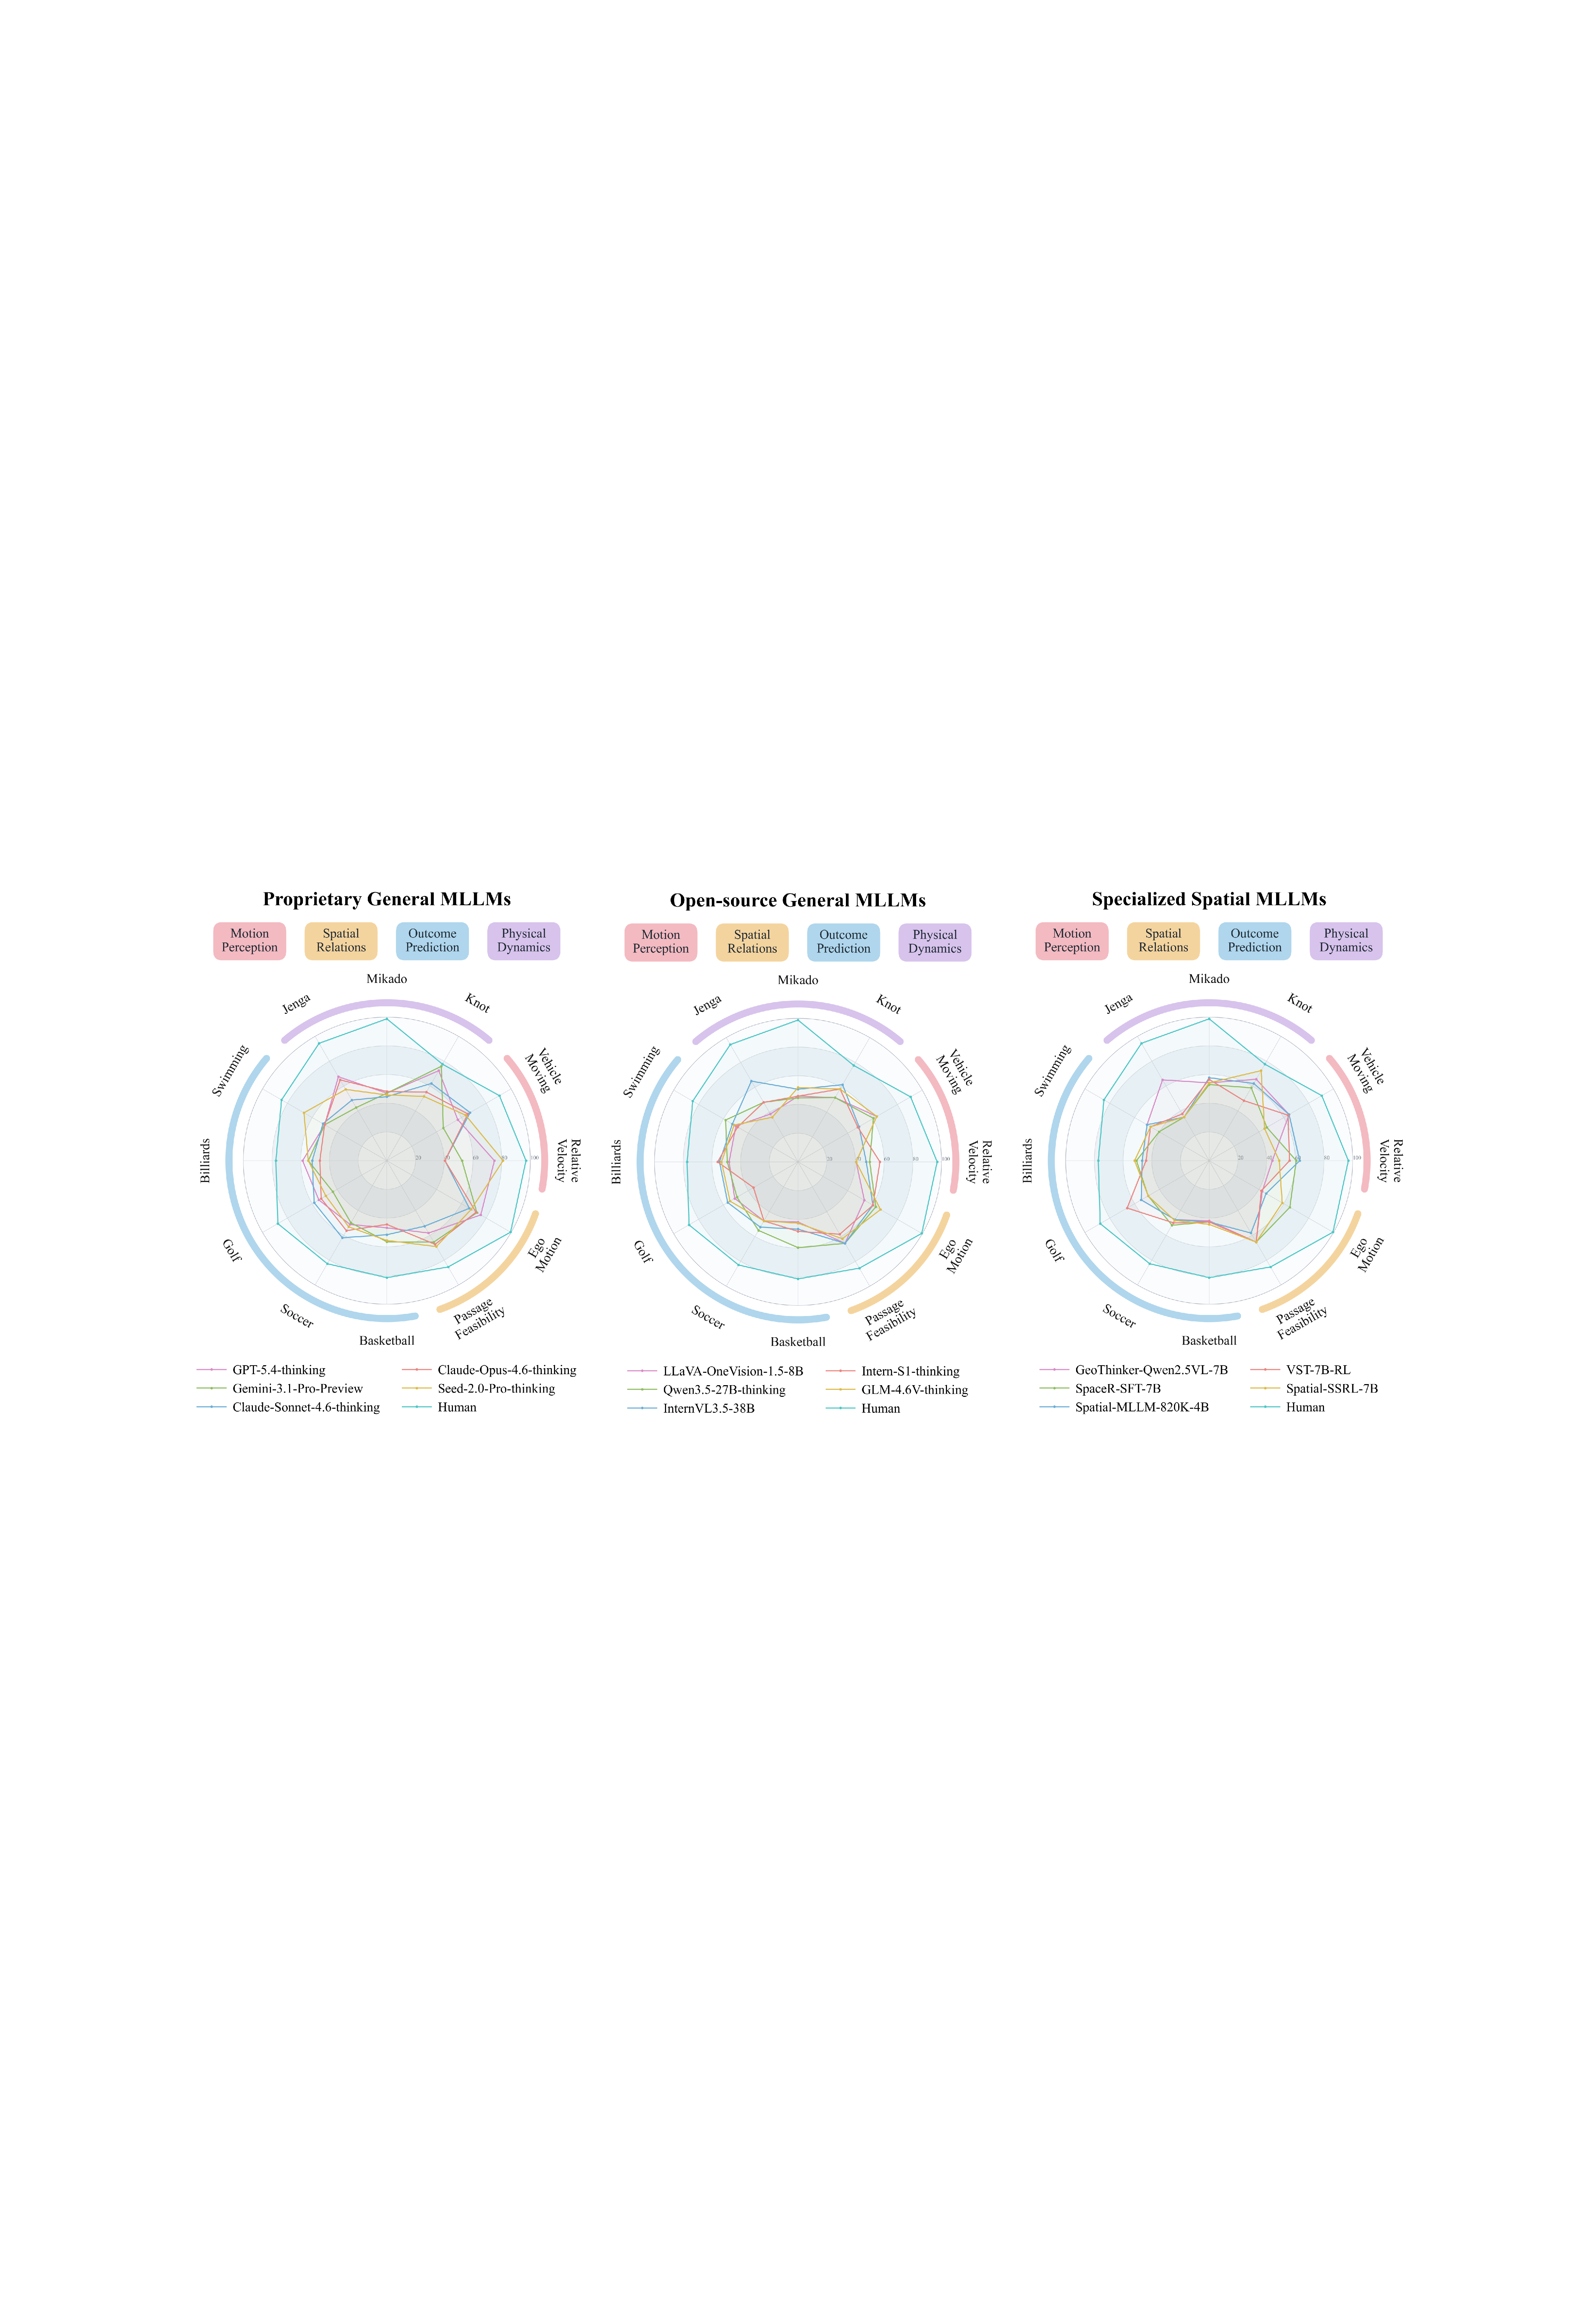
\includegraphics[width=0.9\linewidth]{fig/fig_5.pdf}
  \caption{\textbf{Radar comparison across model groups.} We visualize representative models from proprietary general-purpose MLLMs, open-source general-purpose MLLMs, and specialized spatial MLLMs across the 12 subtasks in ViSTR-Bench. Human performance is shown as a reference, highlighting the substantial gap between current MLLMs and human-level spatial-temporal reasoning.}
  \label{fig:5}
\end{figure}

\subsection{Main Results}
\label{sec:main_results}

Table~\ref{tab:main_results} and Figure~\ref{fig:5} report the comprehensive evaluation results on ViSTR-Bench. We summarize the main observations as follows.

\textbf{Current MLLMs remain far from human-level spatial-temporal reasoning.}
Existing MLLMs achieve limited performance on ViSTR-Bench.
The best-performing model, Seed-2.0-Pro-thinking, obtains an overall accuracy of 59.8\%, only 2.6\% higher than Chance Level (Frequency) and substantially below human performance of 89.0\%.
This large gap indicates that qualitative spatial-temporal reasoning from continuous visual cues remains a challenging problem for current MLLMs.
Moreover, the small margin over the frequency-based baseline suggests that many models still fail to reliably exploit dynamic visual evidence beyond dataset-level answer priors.

\textbf{Proprietary general-purpose MLLMs perform best overall.}
Among all evaluated model groups, proprietary general-purpose MLLMs achieve the best overall results.
Seed-2.0-Pro-thinking and Seed-2.0-Lite-thinking rank first and second, with accuracies of 59.8\% and 59.7\%, respectively, followed by GPT-5.4-thinking at 59.0\% and Claude-Opus-4.6 at 57.0\%.
In contrast, open-source general-purpose MLLMs generally obtain lower performance, with most models falling between 48\% and 55\%.
Notably, within the open-source families, relatively smaller dense models tend to outperform their larger Mixture-of-Experts counterparts.
For instance, Qwen3.5-27B-thinking achieves 55.1\%, surpassing the much larger Qwen3.5-397B-A17B-thinking at 54.3\%.
Similarly, InternVL3.5-38B achieves 54.5\%, outperforming InternVL3.5-241B-A28B at 54.1\%.
This suggests that, for complex continuous visual reasoning tasks, dense activation may provide more stable and reliable temporal representations than sparse routing mechanisms.

\textbf{Spatial MLLMs show limited generalization to dynamic reasoning.}
Although specialized spatial MLLMs are designed to enhance spatial intelligence, they do not show clear advantages on ViSTR-Bench.
The best model in this group, GeoThinker-Qwen2.5VL-7B, achieves only 52.0\% overall accuracy, which is close to random chance and lower than many general-purpose MLLMs.
Moreover, we observe that several specialized spatial MLLMs exhibit biased single-option prediction patterns on certain tasks.
As a result, their performance often matches Chance Level (Frequency) or its complementary value.
This suggests that spatial capability learned from static or geometry-centric training datasets~\citep{SPAR-Bench,LLaVA-Video} does not directly transfer to dynamic spatial-temporal reasoning.
ViSTR-Bench requires models to aggregate temporal evidence, track state changes, and reason about future outcomes or physical interactions, which remain weakly captured by current spatial MLLMs.

\textbf{Thinking mode is helpful but not consistently reliable.}
For models that support built-in thinking modes, enabling thinking often improves overall performance.
For example, GPT-5.4 improves from 54.9\% to 59.0\%, and Seed-2.0-Pro improves from 56.6\% to 59.8\%.
However, the improvement is not universal.
Claude-Opus-4.6 slightly drops from 57.0\% to 56.1\% after enabling thinking, and the gains for MiMo-V2.5 are marginal.
This indicates that explicit reasoning mechanisms can benefit spatial-temporal reasoning, but current thinking modes are not consistently beneficial across models.

\textbf{Performance varies substantially across reasoning dimensions.}
Models generally perform better on Motion Perception and Spatial Relations, where several top models achieve accuracies above 65\% on individual subtasks.
In contrast, Outcome Prediction and Physical Dynamics remain more challenging, with many results close to chance level.
These tasks require anticipating future outcomes or reasoning about latent physical dependencies, rather than merely recognizing visible motion or spatial relations.
This capability imbalance suggests that current MLLMs are better at describing observed dynamics than at performing temporally grounded prediction and intuitive physical reasoning.

\begin{table}[!t]
    \centering
    \caption{
        \textbf{Effect of text-based CoT prompting on ViSTR-Bench.}
        We evaluate Gemini-3.1-Pro-Preview~\citep{Gemini} with \emph{Direct Prompting} and various text-based CoT prompting strategies.
        \emph{Avg.} denotes the overall accuracy (\%) averaged over all question-answer pairs, and $\Delta$ denotes the accuracy change relative to \emph{Direct Prompting}.
        The best and second-best results are highlighted with \bestcap{} and \secondcap{}, respectively.
    }
    \label{tab:text_cot}

    \resizebox{\textwidth}{!}{
    \begin{tabular}{l c c cc cc ccccc ccc}
        \toprule
        \multirow{2}{*}{\textbf{Method}} 
        & \multirow{2}{*}{\textbf{Avg.}} 
        & \multirow{2}{*}{$\boldsymbol{\Delta}$} 
        & \multicolumn{2}{c}{\textbf{Motion Perc.}} 
        & \multicolumn{2}{c}{\textbf{Spat. Rela.}} 
        & \multicolumn{5}{c}{\textbf{Outc. Pred.}}  
        & \multicolumn{3}{c}{\textbf{Phys. Dyna.}} \\
        \cmidrule(lr){4-5} \cmidrule(lr){6-7} \cmidrule(lr){8-12} \cmidrule(lr){13-15}
        & & 
        & \makecell{Vehi.\\Move.} & \makecell{Rela.\\Velo.} 
        & \makecell{Ego\\Motion} & \makecell{Pass.\\Feas.} 
        & Bask. & Soccer & Golf & Bill. & Swim.
        & Jenga & Mikado & Knot \\
        \midrule

        \rowcolor{groupbg}
        \multicolumn{15}{l}{\textbf{Gemini-3.1-Pro-Preview}} \\
        Direct Prompting & 53.6 & - & \best{45.5} & 52.4 & 72.5 & \best{65.5} & \second{56.5} & 50.0 & 43.4 & \best{54.7} & 50.0 & 42.7 & 47.0 & \best{75.9} \\
        Zero-shot CoT & 53.3 & -0.3 & \second{41.1} & \second{56.0} & \second{74.0} & 58.2 & \best{57.3} & 52.5 & \second{50.9} & \second{46.7} & 48.6 & 42.7 & \second{49.4} & 65.5 \\
        Self-Consistency & \second{54.2} & \second{+0.6} & \second{41.1} & 52.4 & \second{74.0} & \second{63.6} & 55.6 & \second{53.2} & 47.2 & \second{46.7} & \second{56.9} & 47.9 & 48.2 & 69.0 \\
        Plan-and-Solve & \second{54.2} & \second{+0.6} & \best{45.5} & 50.0 & \best{76.3} & 61.8 & 54.0 & 51.3 & 49.1 & 44.0 & 45.8 & \second{53.8} & \best{50.6} & 69.0 \\
        Manual CoT & \best{56.0} & \best{+2.4} & \best{45.5} & \best{59.5} & 69.5 & 61.8 & 54.0 & \best{55.1} & \best{58.5} & 41.3 & \best{58.3} & \best{55.6} & \best{50.6} & \second{72.4} \\
        \bottomrule
    \end{tabular}
    }
\end{table}

\subsection{Effect of Text-based CoT Prompting}
\label{sec:text_cot}

We further investigate whether explicit text-based Chain-of-Thought (CoT) prompting can enhance spatial-temporal reasoning on ViSTR-Bench.
Using Gemini-3.1-Pro-Preview as a representative video-based MLLM, we compare four text-based CoT prompting strategies against Direct Prompting, namely Zero-shot CoT~\citep{zero-shot-cot}, Self-Consistency~\citep{self-consistency-coT}, Plan-and-Solve~\citep{plan-and-solve}, and Manual CoT inspired by OmniSpatial~\citep{OmniSpatial}.
Specifically, Zero-shot CoT appends a generic step-by-step reasoning instruction without task-specific design.
Self-Consistency samples multiple reasoning paths by running the Zero-shot CoT prompt over five independent trials and aggregates the final predictions via majority voting.
Plan-and-Solve instructs the model to first formulate a reasoning plan and then execute it to solve the problem.
Manual CoT decomposes each task into human-crafted, task-specific analysis steps tailored to its underlying spatial-temporal reasoning requirement. 
Detailed prompt templates for Manual CoT are provided in Appendix~\ref{sec:detailed_prompt_templates}.

As reported in Table~\ref{tab:text_cot}, text-based CoT prompting brings only limited and strategy-dependent improvements on ViSTR-Bench.
Zero-shot CoT slightly decreases the overall accuracy from 53.6\% to 53.3\% compared with Direct Prompting, suggesting that simply eliciting generic step-by-step reasoning is insufficient for complex video-based spatial-temporal reasoning.
Self-Consistency and Plan-and-Solve both improve the overall accuracy by 0.6\%.
This suggests that aggregating multiple reasoning paths or imposing a more structured reasoning process can help the model to some extent, but the gains remain marginal.
Manual CoT achieves the best overall performance, improving Direct Prompting by 2.4\% and reaching 56.0\%.
By decomposing each task into task-specific reasoning steps, Manual CoT provides stronger guidance for grounding textual reasoning in relevant visual evidence.
Nevertheless, the improvement is still moderate and highly task-dependent.
Moreover, even the best CoT result remains close to the chance-level baselines, indicating that text-based reasoning prompts alone cannot fully compensate for the limitations of current MLLMs in accurate visual perception and temporal grounding.

\begin{table}[!t]
    \centering
    \caption{
        \textbf{Effect of visual input format on ViSTR-Bench.}
        We evaluate Gemini-3.1-Pro-Preview~\citep{Gemini} with different visual input formats.
        \emph{Avg.} denotes the overall accuracy (\%) averaged over all question-answer pairs, and $\Delta$ denotes the accuracy change relative to \emph{Text-only}.
        The best and second-best results are highlighted with \bestcap{} and \secondcap{}, respectively.
    }
    \label{tab:visual_input}

    \resizebox{\textwidth}{!}{
    \begin{tabular}{l c c cc cc ccccc ccc}
        \toprule
        \multirow{2}{*}{\textbf{Input Format}} 
        & \multirow{2}{*}{\textbf{Avg.}} 
        & \multirow{2}{*}{$\boldsymbol{\Delta}$} 
        & \multicolumn{2}{c}{\textbf{Motion Perc.}} 
        & \multicolumn{2}{c}{\textbf{Spat. Rela.}} 
        & \multicolumn{5}{c}{\textbf{Outc. Pred.}}  
        & \multicolumn{3}{c}{\textbf{Phys. Dyna.}} \\
        \cmidrule(lr){4-5} \cmidrule(lr){6-7} \cmidrule(lr){8-12} \cmidrule(lr){13-15}
        & & 
        & \makecell{Vehi.\\Move.} & \makecell{Rela.\\Velo.} 
        & \makecell{Ego\\Motion} & \makecell{Pass.\\Feas.} 
        & Bask. & Soccer & Golf & Bill. & Swim.
        & Jenga & Mikado & Knot \\
        \midrule

        \rowcolor{groupbg}
        \multicolumn{15}{l}{\textbf{Gemini-3.1-Pro-Preview}} \\
        Text-only & 46.4 & - & \second{47.3} & \second{51.2} & 46.6 & 36.4 & 47.6 & 43.0 & \second{52.8} & \second{53.3} & 40.3 & 43.6 & 45.8 & 58.6 \\
        Last Frame & 50.4 & +4.0 & \best{48.2} & 45.2 & 54.2 & 45.5 & \second{50.0} & \second{55.7} & 49.1 & 48.0 & \best{58.3} & \second{44.4} & 45.8 & 65.5 \\
        Shuffled Frames & \second{52.3} & \second{+5.9} & \best{48.2} & \second{51.2} & 60.3 & 56.4 & 49.2 & \best{56.3} & \best{62.3} & 42.7 & 48.6 & \second{44.4} & \best{50.6} & \second{72.4} \\
        Ordered Frames & 51.7 & +5.3 & 46.4 & 47.6 & \second{67.2} & \second{58.2} & 49.2 & 55.1 & 49.1 & \second{53.3} & 47.2 & \best{48.7} & 36.1 & 62.1 \\
        Original Video & \best{53.6} & \best{+7.2} & 45.5 & \best{52.4} & \best{72.5} & \best{65.5} & \best{56.5} & 50.0 & 43.4 & \best{54.7} & \second{50.0} & 42.7 & \second{47.0} & \best{75.9} \\
        \bottomrule
    \end{tabular}
    }
\end{table}

\subsection{Effect of Visual Input Format}
\label{sec:visual_input}

We further study how different visual input formats affect model performance on ViSTR-Bench.
Using Gemini-3.1-Pro-Preview as the evaluated model, we compare five input settings: text-only input, the last frame only, shuffled frames with disrupted temporal order, ordered frames uniformly sampled from the video, and the original video input.
As reported in Table~\ref{tab:visual_input}, all visual input formats consistently outperform the text-only setting, showing that visual evidence provides useful cues beyond language priors.
Multi-frame inputs bring larger gains, with ordered frames and shuffled frames improving over the last-frame setting by 1.3\% and 1.9\%, respectively, suggesting that the model can benefit from observing multiple visual states.
However, shuffled frames slightly outperform ordered frames in overall accuracy, indicating that the model does not reliably exploit the continuous temporal order among frames.
This suggests that current MLLMs may capture coarse temporal-related cues from multiple frames, but still struggle to reason over continuous visual dynamics.
Original video input achieves the best performance, reaching 53.6\% overall accuracy.
These results indicate that video input provides the most complete visual evidence, while effective reasoning from continuous visual cues remains challenging for current MLLMs.


%% ============================================================
%%  5. Analysis
%% ============================================================
% \section{Analysis}

% \subsection{Computational Efficiency}

% Our method achieves a favorable trade-off between accuracy and computational
% cost. Compared to Method-B, Colab-Net uses $35\%$ fewer FLOPs while
% achieving $4.4\%$ higher accuracy on Dataset-A.

% \subsection{Qualitative Results}

% Figure~\ref{fig:qualitative} shows qualitative comparisons between our method
% and two baseline approaches. Our method produces more accurate and coherent
% outputs, particularly in challenging cases with ambiguous inputs.

% \begin{figure}[htbp]
%   \centering
%   \fcolorbox{colabPrimary!30}{colabLightGray}{%
%     \parbox{0.88\linewidth}{%
%       \vspace{3cm}
%       \centering\color{colabGray}
%       {\sffamily\large [Figure Placeholder]}\\[4pt]
%       {\small Replace this box with your actual figure using
%        \texttt{\textbackslash includegraphics}.}
%       \vspace{3cm}
%     }%
%   }
%   \caption{Qualitative comparison of our method versus baselines on challenging
%            examples from Dataset-A. Our approach produces more coherent and
%            accurate predictions.}
%   \label{fig:qualitative}
% \end{figure}

%% ============================================================
%%  6. Discussion
%% ============================================================
% \section{Discussion}

% Our results demonstrate the effectiveness of combining hierarchical feature
% extraction with contrastive pre-training for representation learning.
% Several observations merit further discussion.

% While our method achieves strong results across five benchmarks, we note
% two limitations: (1) the pre-training phase requires significant compute
% resources, and (2) performance gains are smaller on tasks with limited
% training data ($<$1000 samples).

% The scalability of our approach suggests promising directions for future work,
% including extension to multimodal settings and adaptation to low-resource
% scenarios through few-shot learning.

%% ============================================================
%%  7. Conclusion
%% ============================================================

\section{Conclusion}
In this paper, we introduced ViSTR-Bench, a visual spatial-temporal reasoning benchmark designed to evaluate whether MLLMs can reason from continuous visual cues in dynamic scenes. 
Unlike prior benchmarks that mainly focus on static spatial attributes, low-level temporal perception, or quantitative prediction, ViSTR-Bench emphasizes temporal evidence, reasoning-oriented task design, and qualitative evaluation. It covers four complementary dimensions, with 12 subtasks and 1,093 high-quality video question-answer pairs across tabletop, indoor, and outdoor scenarios. Through comprehensive evaluations of proprietary, open-source, and specialized spatial MLLMs, we find that current models remain substantially below human performance. We hope ViSTR-Bench can serve as a diagnostic testbed for future research on physically grounded multimodal intelligence, embodied AI, and dynamic world modeling.


% \paragraph{Acknowledgments.}
% This research is supported in part by the Zhongguancun Academy (Grant No. 02012404), National Key R\&D Program of China (2022ZD0115502), National Natural Science Foundation of China (No. 62461160308, No. 62576024, U23B2010), ``the Fundamental Research Funds for the Central Universities'' (No. 501RCQD2025), ``Pioneer'' and ``Leading Goose'' R\&D Program of Zhejiang (No. 2024C01161), Beijing Natural Science Foundation (QY25227), Ningbo Science and Technology Innovation 2025 Major Project (2025Z034), NSFCRGC Project (N CUHK498/24).

%% ============================================================
%%  References
%% ============================================================
{\small
\bibliographystyle{\colabbibstyle}
\bibliography{references}
}

%% ============================================================
%%  Appendix  (Requirement 6 — tcolorbox demo)
%% ============================================================

\clearpage

{
    \hypersetup{linkcolor=black}
    \tableofcontents
}

\clearpage
\appendix
% \setcounter{page}{1}
% \maketitlesupplementary

\section*{Appendix}

\section{Detailed Data Sources}
\label{sec:detailed_data_sources}

Table~\ref{tab:detailed_data_sources} summarizes the task-level data source statistics of ViSTR-Bench.
For each subtask, we report the total number of video question-answer pairs and further categorize them by data source, including public datasets, curated web videos, and self-collected recordings.
We then briefly introduce the public datasets used to construct ViSTR-Bench.

\noindent\textbf{Waymo Open Dataset}~\citep{Waymo} is a large-scale autonomous driving dataset comprising 1,150 driving segments. Each segment lasts approximately 20 seconds and provides synchronized multi-view videos with rich annotations for traffic agents, including vehicles, pedestrians, and cyclists. The dataset is widely used for autonomous driving perception tasks such as 3D object detection, object tracking, and motion forecasting.
In ViSTR-Bench, we use videos from the Waymo Open Dataset~\citep{Waymo} for driving-related motion perception tasks, including Vehicle Movement and Relative Velocity. We also leverage the available vehicle annotations to localize target vehicles and overlay visual prompts on the corresponding video frames.

\noindent\textbf{ScanNet}~\citep{ScanNet} is a richly annotated RGB-D dataset of real-world indoor scenes, comprising more than 1,500 indoor scans and over 2.5 million RGB-D views. The dataset covers diverse indoor environments, such as bedrooms, offices, and living rooms. ScanNet is widely used for 3D reconstruction, semantic segmentation, and instance segmentation.
In ViSTR-Bench, we use ScanNet~\citep{ScanNet} as one of the data sources for the Ego Motion task. Given an indoor egocentric video and a target object, the model is required to infer the final spatial relationship between the observing camera and the target object.

\noindent\textbf{ScanNet++}~\citep{ScanNet++} is an extension of ScanNet~\citep{ScanNet}, offering more detailed geometry, denser visual observations, and more complete scene coverage.
It contains 460 indoor scenes, covering more than 1,000 object categories and over 21,000 object instances.
In ViSTR-Bench, we use ScanNet++~\citep{ScanNet++} as an additional data source for the Ego Motion task.

\noindent\textbf{ARKitScenes}~\citep{ARKitScenes} is a large-scale indoor RGB-D dataset captured using mobile devices equipped with LiDAR sensors. It contains 5,047 captures from 1,661 unique indoor scenes. ARKitScenes~\citep{ARKitScenes} is commonly used for 3D reconstruction, depth estimation, and indoor object detection.
In ViSTR-Bench, we use ARKitScenes~\citep{ARKitScenes} as another data source for the Ego Motion task.

\noindent\textbf{Ego4D}~\citep{Ego4D} is a large-scale egocentric video dataset that records unscripted daily human activities from a first-person perspective. It contains more than 3,700 hours of video collected by 926 participants across 74 locations in nine countries. The dataset covers diverse activities in homes, workplaces, outdoor environments, and recreational scenes. Ego4D~\citep{Ego4D} is widely used for egocentric video understanding, activity recognition, and human-object interaction analysis.
In ViSTR-Bench, we use Ego4D~\citep{Ego4D} as a public data source for outcome prediction tasks, including Basketball Shot and a subset of Billiards Shot examples.

\begin{table}[!t]
    \centering
    \caption{
        \textbf{Task-level data source statistics of ViSTR-Bench.}
        For each subtask, we report the total number of QA pairs and the number of samples collected from public datasets, curated web videos, and self-collected recordings.
    }
    \label{tab:detailed_data_sources}
    \small
    \begin{tabular}{lrrrr}
        \toprule
        \textbf{Task} & \textbf{Total} & \textbf{Public Datasets} & \textbf{Web Videos} & \textbf{Self-collected} \\
        \midrule

        \multicolumn{5}{l}{\textbf{Motion Perception}} \\
        \quad Vehicle Movement & 112 & 112 & 0 & 0 \\
        \quad Relative Velocity & 84 & 84 & 0 & 0 \\
        \midrule

        \multicolumn{5}{l}{\textbf{Spatial Relations}} \\
        \quad Ego Motion & 131 & 131 & 0 & 0 \\
        \quad Passage Feasibility & 55 & 0 & 0 & 55 \\
        \midrule

        \multicolumn{5}{l}{\textbf{Outcome Prediction}} \\
        \quad Basketball Shot & 124 & 124 & 0 & 0 \\
        \quad Soccer Shot & 158 & 0 & 158 & 0 \\
        \quad Golf Shot & 53 & 0 & 53 & 0 \\
        \quad Billiards Shot & 75 & 28 & 47 & 0 \\
        \quad Swimming Race & 72 & 0 & 72 & 0 \\
        \midrule

        \multicolumn{5}{l}{\textbf{Physical Dynamics}} \\
        \quad Jenga Stability & 117 & 0 & 0 & 117 \\
        \quad Mikado Dependency & 83 & 0 & 0 & 83 \\
        \quad Knot Type & 29 & 0 & 23 & 6 \\
        \midrule
        
        \textbf{Total} & \textbf{1093} & \textbf{479} & \textbf{353} & \textbf{261} \\
        \bottomrule
    \end{tabular}
\end{table}

\section{Detailed Prompt Templates}
\label{sec:detailed_prompt_templates}

\begin{table}[!t]
    \centering
    \caption{
        \textbf{Direct Prompting templates used in ViSTR-Bench.}
        We list the direct prompting template for each subtask.
        Placeholders such as \texttt{\{TARGET\}}, \texttt{\{OPTION\_A\}}, and \texttt{\{OPTION\_B\}} are replaced with instance-specific metadata during QA pair generation.
        % Most subtasks use fixed binary answer spaces, while Ego Motion and Swimming Race construct binary choices from relative-position labels and lane numbers, respectively.
    }
    \label{tab:direct_prompt_templates}
    \small
    \begin{tabular}{p{0.20\textwidth} p{0.70\textwidth}}
        \toprule
        \textbf{Task} & \textbf{Prompt Template} \\
        \midrule

        \multicolumn{2}{l}{\textbf{Motion Perception}} \\
        \quad Vehicle Movement
        & This is a driving video. Please determine whether the vehicle in the green box shows subtle movement during the video. Answer Yes or No. \\

        \quad Relative Velocity
        & This is a driving video. Please determine which vehicle is moving faster based on their motion over time: the vehicle in the green box or the vehicle in the blue box. Answer Green or Blue. \\
        \midrule

        \multicolumn{2}{l}{\textbf{Spatial Relations}} \\
        \quad Ego Motion
        & This is a video recorded by a moving camera in an indoor scene. The target object is the \texttt{\{TARGET\}}. Please determine the final position of the target object relative to the camera. Is it \texttt{\{OPTION\_A\}} or \texttt{\{OPTION\_B\}}? Answer \texttt{\{OPTION\_A\}} or \texttt{\{OPTION\_B\}}. \\

        \quad Passage Feasibility
        & This is a video of a vehicle and traffic cones placed near its driving path. Please predict whether the vehicle can pass the cone-constrained area without touching any cone. Answer Yes or No. \\
        \midrule

        \multicolumn{2}{l}{\textbf{Outcome Prediction}} \\
        \quad Basketball Shot
        & This is a video of a basketball shot. Please predict whether the basketball will go into the hoop. Answer Yes or No. \\

        \quad Soccer Shot
        & This is a video of a soccer free kick. Please predict whether the ball will go into the goal based on its trajectory, ignoring the goalkeeper and any defensive interference. Answer Yes or No. \\

        \quad Golf Shot
        & This is a video of a golf shot. Please predict whether the golf ball will go into the hole based on its observed trajectory. Answer Yes or No. \\

        \quad Billiards Shot
        & This is a video of billiards. Please predict whether the target ball will go into the pocket based on its current trajectory. Answer Yes or No. \\

        \quad Swimming Race
        & This is a video of a swimming race. The swimmer at the top of the frame is in lane 1, and the lane numbers increase from top to bottom. Please determine which swimmer will reach the finish line first between lane \texttt{\{OPTION\_A\}} and lane \texttt{\{OPTION\_B\}}. Answer \texttt{\{OPTION\_A\}} or \texttt{\{OPTION\_B\}}. \\
        \midrule

        \multicolumn{2}{l}{\textbf{Physical Dynamics}} \\
        \quad Jenga Stability
        & This is a video of a Jenga game. Please predict whether the tower will remain stable after the block that the hand is trying to pull out is removed. Answer Yes or No. \\

        \quad Mikado Dependency
        & This is a video of a Mikado game. Please predict whether the stick indicated by the pointing stick can be picked up without touching any other sticks. Answer Yes or No. \\

        \quad Knot Type
        & This is a video of knot manipulation. Please determine whether the knot is a slip knot (can be undone by pulling one end) or a fixed knot (cannot be undone and remains tight when pulled). Answer Slip or Fixed. \\
        \bottomrule
    \end{tabular}
\end{table}

\subsection{Direct Prompting}

Table~\ref{tab:direct_prompt_templates} presents the Direct Prompting templates used in ViSTR-Bench.
Each prompt specifies the visual context, the reasoning target, and the required answer format for the corresponding subtask.
Placeholders such as \texttt{\{TARGET\}}, \texttt{\{OPTION\_A\}}, and \texttt{\{OPTION\_B\}} are replaced with instance-specific metadata during QA pair generation.
Most subtasks adopt fixed binary answer spaces, including Yes/No for judgment tasks, Green/Blue for comparing prompted vehicles, and Slip/Fixed for knot classification.
For the remaining subtasks, Ego Motion constructs binary choices from relative-position labels, including front-left, front-right, back-left, and back-right, whereas Swimming Race constructs binary choices from lane numbers.

\subsection{Manual CoT}

Inspired by OmniSpatial~\citep{OmniSpatial}, Manual CoT explicitly decomposes each task into visually grounded intermediate reasoning steps.
This design differs from existing methods such as Zero-shot CoT~\citep{zero-shot-cot}, Self-Consistency~\citep{self-consistency-coT}, and Plan-and-Solve~\citep{plan-and-solve}, which rely on generic reasoning instructions or repeated sampling with the same prompt.
Specifically, we manually design a task-specific reasoning procedure for each subtask in ViSTR-Bench, guiding the model to first identify the relevant visual target, then track task-specific spatial-temporal evidence across the video, and finally produce the prediction using the prescribed answer format.
The complete Manual CoT prompt templates are shown in Figures~\ref{fig:6}-\ref{fig:17}.

\section{Model and Inference Details}
\label{sec:model_inference_details}

For general-purpose MLLMs, we adopt different input formats depending on whether each model natively supports video input.
For Gemini-3/3.1~\citep{Gemini}, Seed-2.0~\citep{Seed}, MiMo-V2/V2.5~\citep{MiMo-V2-Omni,MiMo-V2.5}, Qwen3.5~\citep{Qwen3.5}, and GLM-4.6V~\citep{GLM-4.6V}, we directly provide the original video clip as the visual input.
The maximum video resolution is constrained to $1920 \times 1280$, and the maximum Base64-encoded video size is set to 10 MB.
For GPT-5.4~\citep{GPT-5}, Claude-4.6~\citep{Claude}, Intern-S1~\citep{Intern-S1,Intern-S1-Pro}, and InternVL3.5~\citep{InternVL3.5}, we convert each video into a sequence of sampled frames.
Specifically, we uniformly sample 16 frames from each video and constrain the maximum image resolution to $1280 \times 720$.
The sampled frames are provided together with a short textual instruction indicating that they are sampled from the same video and arranged in chronological order, followed by the task question.
For model-specific inference settings, we set the thinking level of GPT-5.4~\citep{GPT-5} to \texttt{xhigh}.
For Gemini-3/3.1~\citep{Gemini}, we set the temperature to 1.0, top-$p$ to 0.95, top-$k$ to 64, the maximum output length to 65,536 tokens, and the thinking level to \texttt{high}.
For Claude-4.6~\citep{Claude}, we set the maximum output length to 16,000 tokens and the thinking budget to 1,024 tokens.
Finally, for specialized spatial MLLMs, we run their official source code with the default inference settings.

\section{Error Analysis}
\label{sec:error_analysis}

To better investigate why current MLLMs exhibit limited performance on ViSTR-Bench, we conduct an error analysis of the 481 incorrect predictions made by Gemini-3.1-Pro-Preview~\citep{Gemini} under the Manual CoT setting.
For each incorrect prediction, we assign one primary error type based on the task definition, the ground-truth answer, and the reasoning steps generated by the model following the Manual CoT prompt.

\subsection{Error Categorization}

We define six task-agnostic primary error types to characterize the major failure modes observed across different subtasks.
Representative examples for each error category are illustrated in Figure~\ref{fig:18}.

\noindent\textbf{Target Identification Error.} % Billiards Shot
The model fails to reliably identify the target object specified in the question.
Typical examples include confusing the target ball in Billiards, mixing up lane numbers in Swimming Race, and localizing the wrong Jenga block or Mikado stick.

\noindent\textbf{Target Tracking Error.} % Basketball Shot, Soccer Shot, Golf Shot, Billiards Shot
The model correctly identifies the target but fails to continuously track its trajectory over time.
Typical examples include losing track of a moving ball or confusing its position across consecutive frames.

\noindent\textbf{Motion State Error.} % Vehicle Movement, Relative Velocity
The model correctly identifies the prompted vehicles but misjudges their motion state.
Typical cases include missing subtle vehicle movement in Vehicle Movement or incorrectly identifying the faster vehicle in Relative Velocity.

\noindent\textbf{Outcome Reasoning Error.} % Basketball Shot, Soccer Shot, Golf Shot, Billiards Shot, Swimming Race
The model correctly observes the current motion or state but fails to infer the correct final outcome.
Typical cases include incorrectly predicting whether a shot will succeed or which swimmer will reach the finish line first.

\noindent\textbf{Spatial Relation Error.} % Ego Motion, Passage Feasibility
The model incorrectly estimates spatial relations between the target and reference objects.
Representative cases include reversing observer-centric directions in Ego Motion or misjudging whether a vehicle has sufficient spatial clearance to pass through a cone-constrained region in Passage Feasibility.

\noindent\textbf{Physical Interaction Error.} % Jenga Stability, Mikado Dependency, Knot Type
The model incorrectly reasons about latent physical properties, dependencies, or stability conditions.
For example, the model may misjudge whether a Mikado stick is blocked by another stick, whether a Jenga block is load-bearing, or whether a specific knot can be released by pulling one end.

\begin{table}[!t]
    \centering
    \caption{
        \textbf{Distribution of primary error types.}
        We analyze the 481 incorrect predictions made by Gemini-3.1-Pro-Preview~\citep{Gemini} under the Manual CoT setting.
        Each incorrect prediction is assigned one primary error type.
    }
    \label{tab:error_distribution}
    \small
    \begin{tabular}{lrr}
        \toprule
        \textbf{Primary Error Type} & \textbf{\#Errors} & \textbf{Ratio} \\
        \midrule
        Outcome Reasoning Error & 156 & 32.4\% \\
        Physical Interaction Error & 101 & 21.0\% \\
        Motion State Error & 95 & 19.7\% \\
        Spatial Relation Error & 61 & 12.7\%  \\
        Target Tracking Error & 59 & 12.3\% \\
        Target Identification Error & 9 & 1.9\%  \\
        \midrule
        \textbf{Total} & \textbf{481} & \textbf{100.0\%} \\
        \bottomrule
    \end{tabular}
\end{table}

\subsection{Error Statistics}

Table~\ref{tab:error_distribution} reports the distribution of the primary error types.
\emph{Outcome Reasoning Error} is the most frequent category. These cases indicate that even when the model captures the current motion or intermediate state, it often fails to extrapolate these cues to the correct final outcome.
\emph{Physical Interaction Error} is mainly observed in Jenga Stability, Mikado Dependency, and Knot Type, showing that current MLLMs have limited ability to infer latent physical properties, object dependencies, and stability conditions.
\emph{Motion State Error} is the third-largest category, suggesting that current MLLMs still struggle to determine whether a prompted object is moving and to compare motion-related attributes such as relative speed.
\emph{Spatial Relation Error} mainly arises in Ego Motion and Passage Feasibility, where the model either reverses observer-centric directions or misjudges the spatial clearance between a vehicle and surrounding obstacles.
\emph{Target Tracking Error} reflects failures in continuously following the target trajectory over time, especially in ball-centric outcome prediction tasks.
\emph{Target Identification Error} accounts for only 9 cases, mostly occurring in Billiards, where the model confuses the target ball with other balls on the table.
Overall, the error distribution shows that the main bottlenecks of current MLLMs on ViSTR-Bench are not simple failures to recognize target objects.
Instead, the dominant limitations lie in predicting motion states and attributes, tracking dynamic visual evidence over time, extrapolating observed states to future outcomes, and reasoning about latent physical interactions.

\section{Preliminary Exploration on Model Improvement}
\label{sec:model_improvement}

The error analysis shows that current MLLMs still struggle to reason from continuous visual cues in dynamic scenes.
Based on these observations, we discuss several complementary directions for improving model performance.
First, a data-centric direction is to construct larger-scale training data specifically designed for dynamic spatial-temporal reasoning.
Although current MLLMs are trained on massive image-text and video-text corpora, existing datasets~\citep{SPAR-Bench,LLaVA-Video} mainly focus on static visual recognition or general video understanding, and provide limited supervision for fine-grained dynamic reasoning.
Second, an input-centric direction is to enrich the visual input with more explicit spatial evidence beyond the original camera trajectory.
For example, auxiliary novel views can be rendered from the reconstructed scene and added to the original video, providing complementary geometric and layout cues that are not directly observed from the captured viewpoints.
Third, a tool-augmented direction is to build agentic systems that decompose complex video reasoning problems into intermediate subproblems and use external tools to extract task-relevant visual evidence.
For instance, detectors and trackers can localize target objects, optical flow can estimate motion patterns, and 3D reconstruction can recover scene geometry.
This paradigm is promising because it offloads low-level visual perception to specialized tools, allowing MLLMs to focus more on high-level spatial-temporal reasoning.

As a preliminary exploration, we investigate the input-centric direction on the Ego Motion task.
We select GPT-5.4-thinking~\citep{GPT-5}, the best-performing model on this task, and augment the 16-frame baseline with 10 rendered auxiliary views.
Specifically, we first reconstruct the 3D scene from the original video using VGGT-$\Omega$~\citep{VGGT-Omega}, and then render novel views as additional spatial evidence for the model.
This simple augmentation improves the accuracy from 75.6\% to 80.2\%, indicating that auxiliary rendered views can make useful spatial cues more accessible to current MLLMs.
Rather than proposing a complete solution, this preliminary study aims to examine whether geometry-enhanced inputs can benefit dynamic scene reasoning, thereby highlighting a promising direction for improving the spatial-temporal reasoning ability of current MLLMs.

\section{Qualitative Visualizations}
\label{sec:visualization}

We provide qualitative visualizations for all 12 tasks in ViSTR-Bench.
For each task, we select one representative example and visualize the model outputs from GPT-5.4-thinking~\citep{GPT-5}, Gemini-3.1-Pro-Preview~\citep{Gemini}, and Claude-Opus-4.6-thinking~\citep{Claude}.
The results are shown in Figures~\ref{fig:19}-\ref{fig:30}.

\section{Limitations and Future Work}
\label{sec:limitations_future_work}

While ViSTR-Bench provides a diagnostic testbed for visual spatial-temporal reasoning, it also has several limitations that motivate future research.

\noindent\textbf{Task and data coverage.}
ViSTR-Bench covers 12 subtasks across tabletop, indoor, and outdoor scenarios, but it is not intended to exhaust all forms of spatial-temporal reasoning in the physical world.
The current benchmark focuses on relatively short clips with clearly specified targets and binary decisions.
In contrast, many real-world embodied tasks require longer-horizon planning, multi-agent interaction, and adaptation to continuously changing goals.
Future work can extend ViSTR-Bench to broader scene categories, longer temporal contexts, and more interactive scenarios, enabling evaluation under settings closer to robotics, autonomous driving, and embodied AI applications.

\noindent\textbf{Evaluation format.}
All tasks in ViSTR-Bench are formulated as qualitative binary-choice questions.
This design reduces annotation ambiguity, mitigates the impact of minor numerical errors, and enables controlled comparisons across different MLLMs.
However, binary accuracy only measures the final decision and cannot fully capture graded spatial-temporal understanding or the correctness of intermediate reasoning steps.
Future benchmarks may combine qualitative decisions with richer answer formats, such as open-ended explanations or structured annotations of object states, spatial relations, and physical dependencies.

\noindent\textbf{Model improvement.}
Our experiments and error analysis show that current MLLMs mainly struggle with target tracking, outcome extrapolation, spatial relation estimation, and latent physical interaction reasoning.
The preliminary exploration in Appendix~\ref{sec:model_improvement} suggests that richer spatial evidence can provide useful cues, but it remains only an initial step toward improving dynamic scene reasoning.
Promising directions include constructing larger training corpora for dynamic spatial-temporal reasoning, integrating external perception tools such as object trackers, optical flow estimators, and 3D reconstruction modules, and developing world-modeling mechanisms that explicitly maintain object states and physical relations over time.
We hope ViSTR-Bench can support these directions by serving not only as an evaluation benchmark, but also as a diagnostic resource for identifying underdeveloped components of dynamic visual reasoning.

\begin{figure}[p]
  \centering
  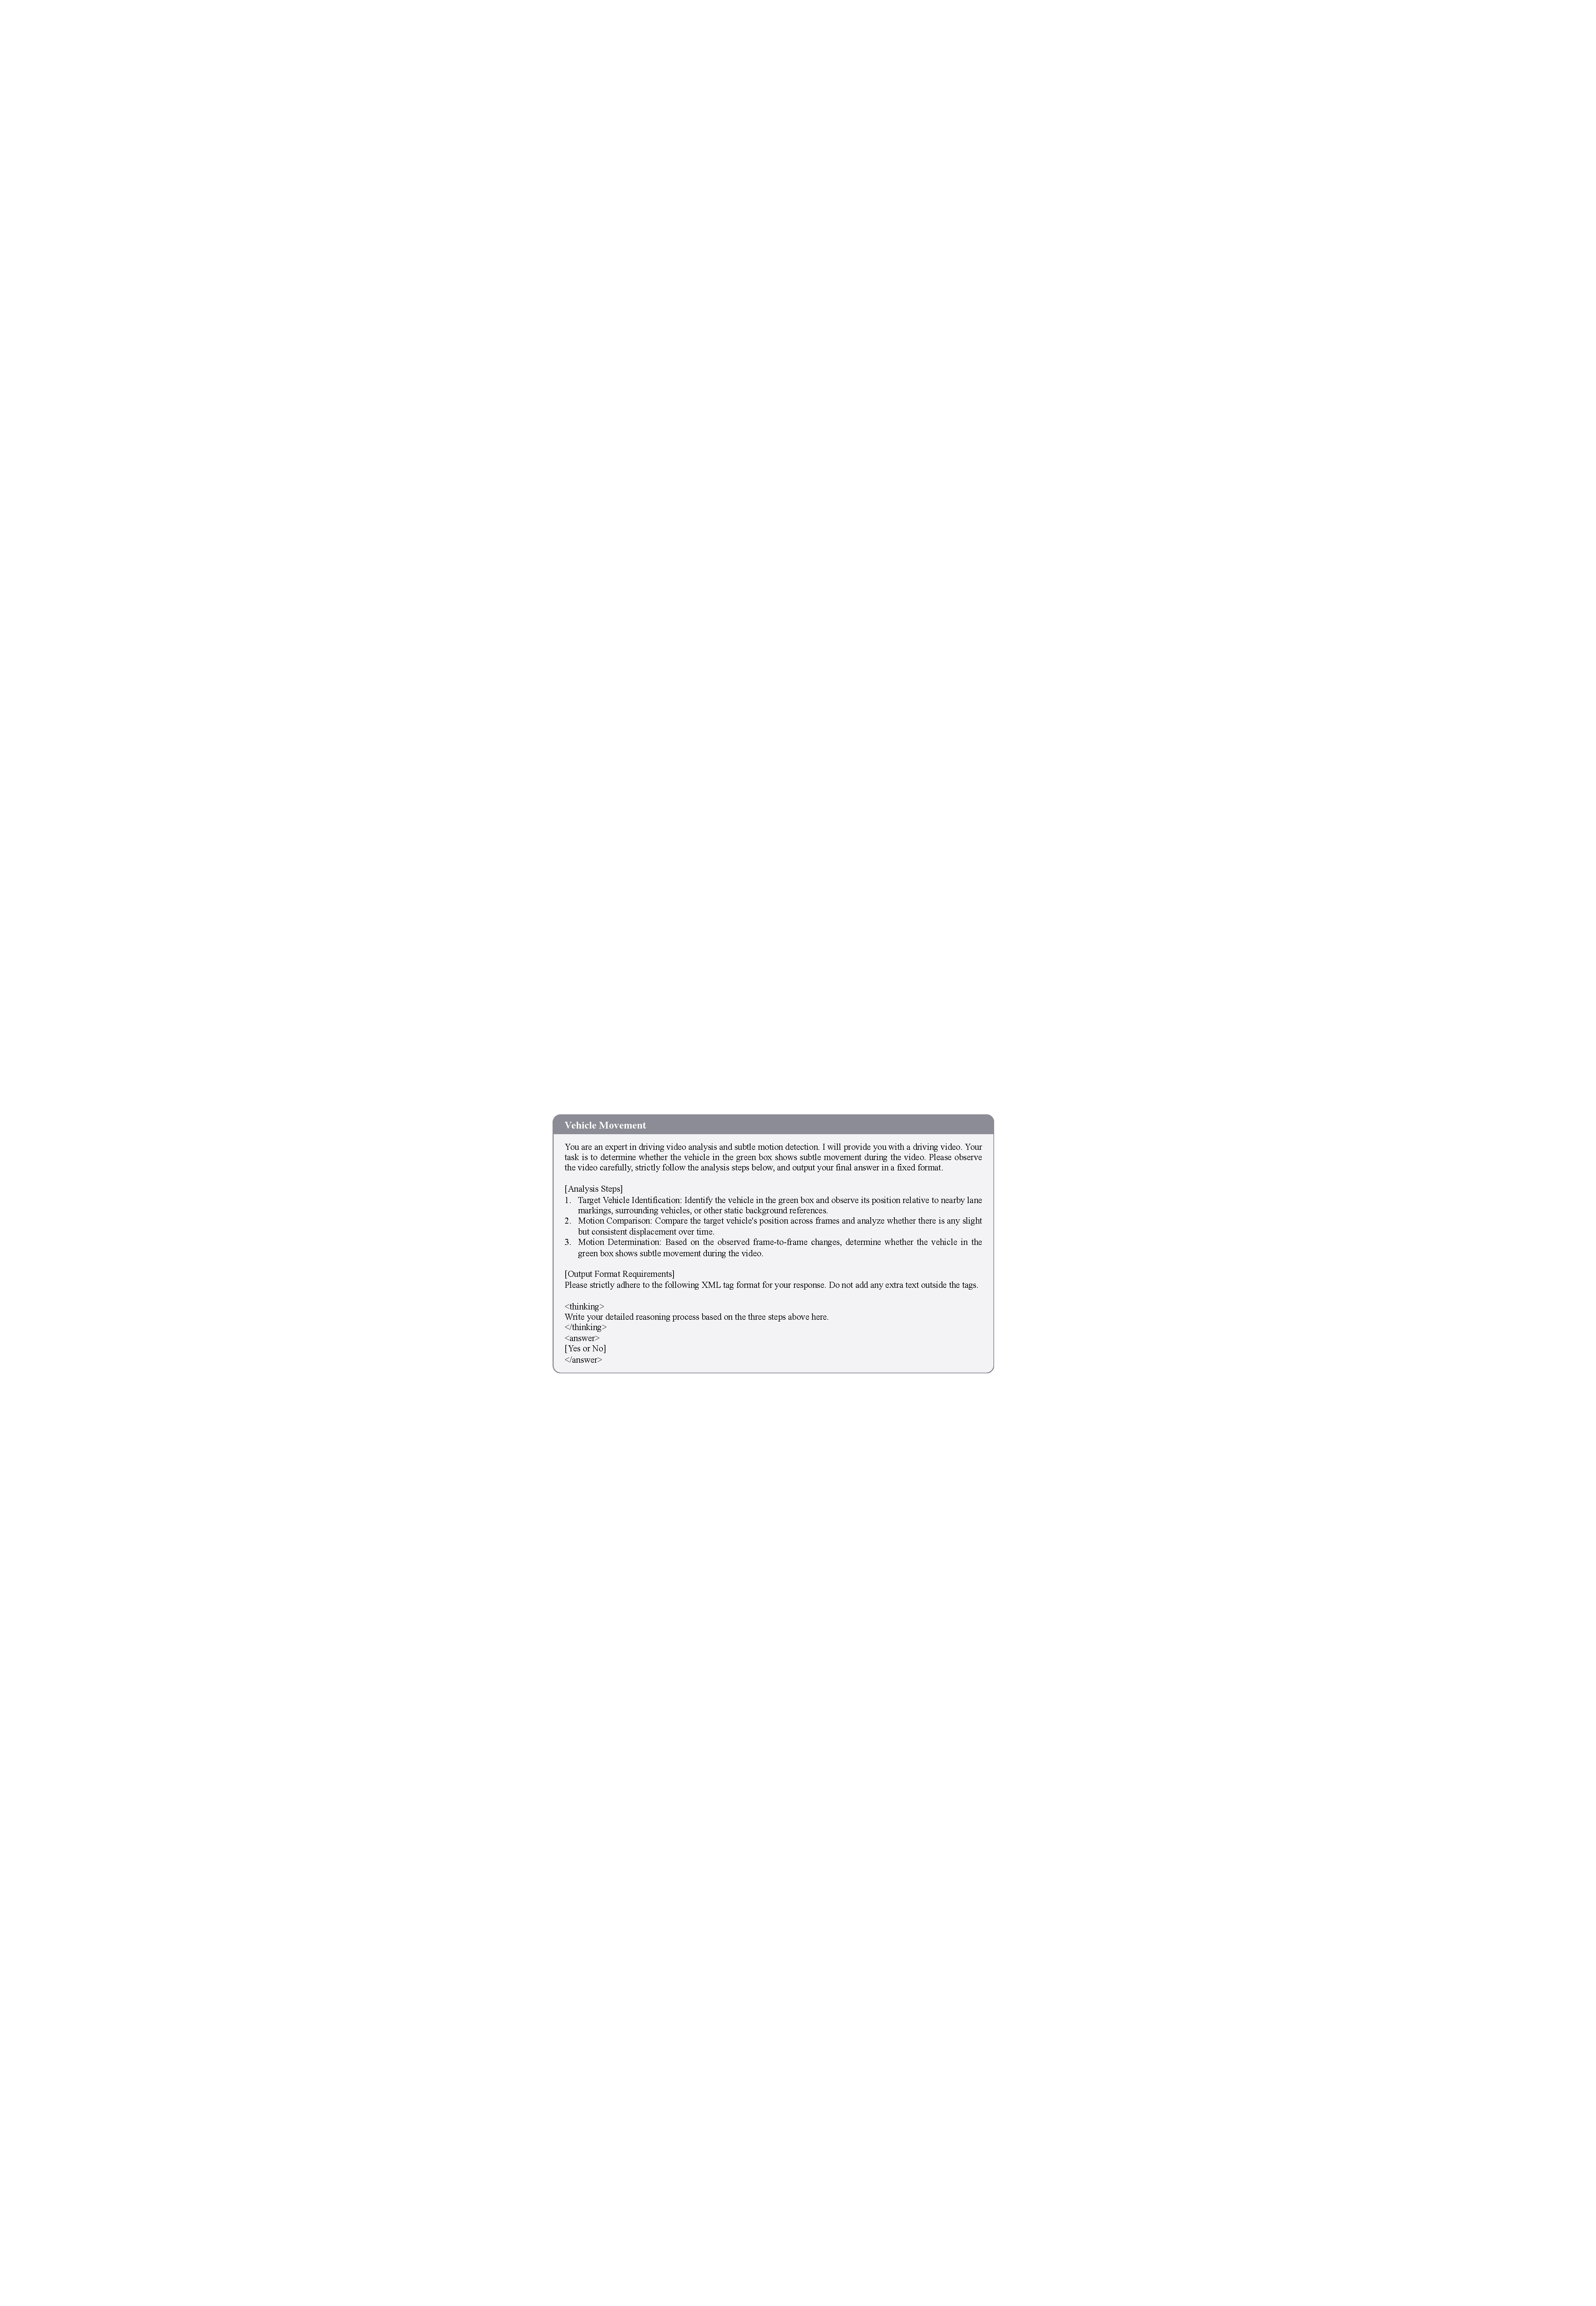
\includegraphics[width=0.95\linewidth]{fig/fig_6.pdf}
  \caption{\textbf{Manual CoT prompt template for Vehicle Movement.}}
  \label{fig:6}
\end{figure}

\begin{figure}[p]
  \centering
  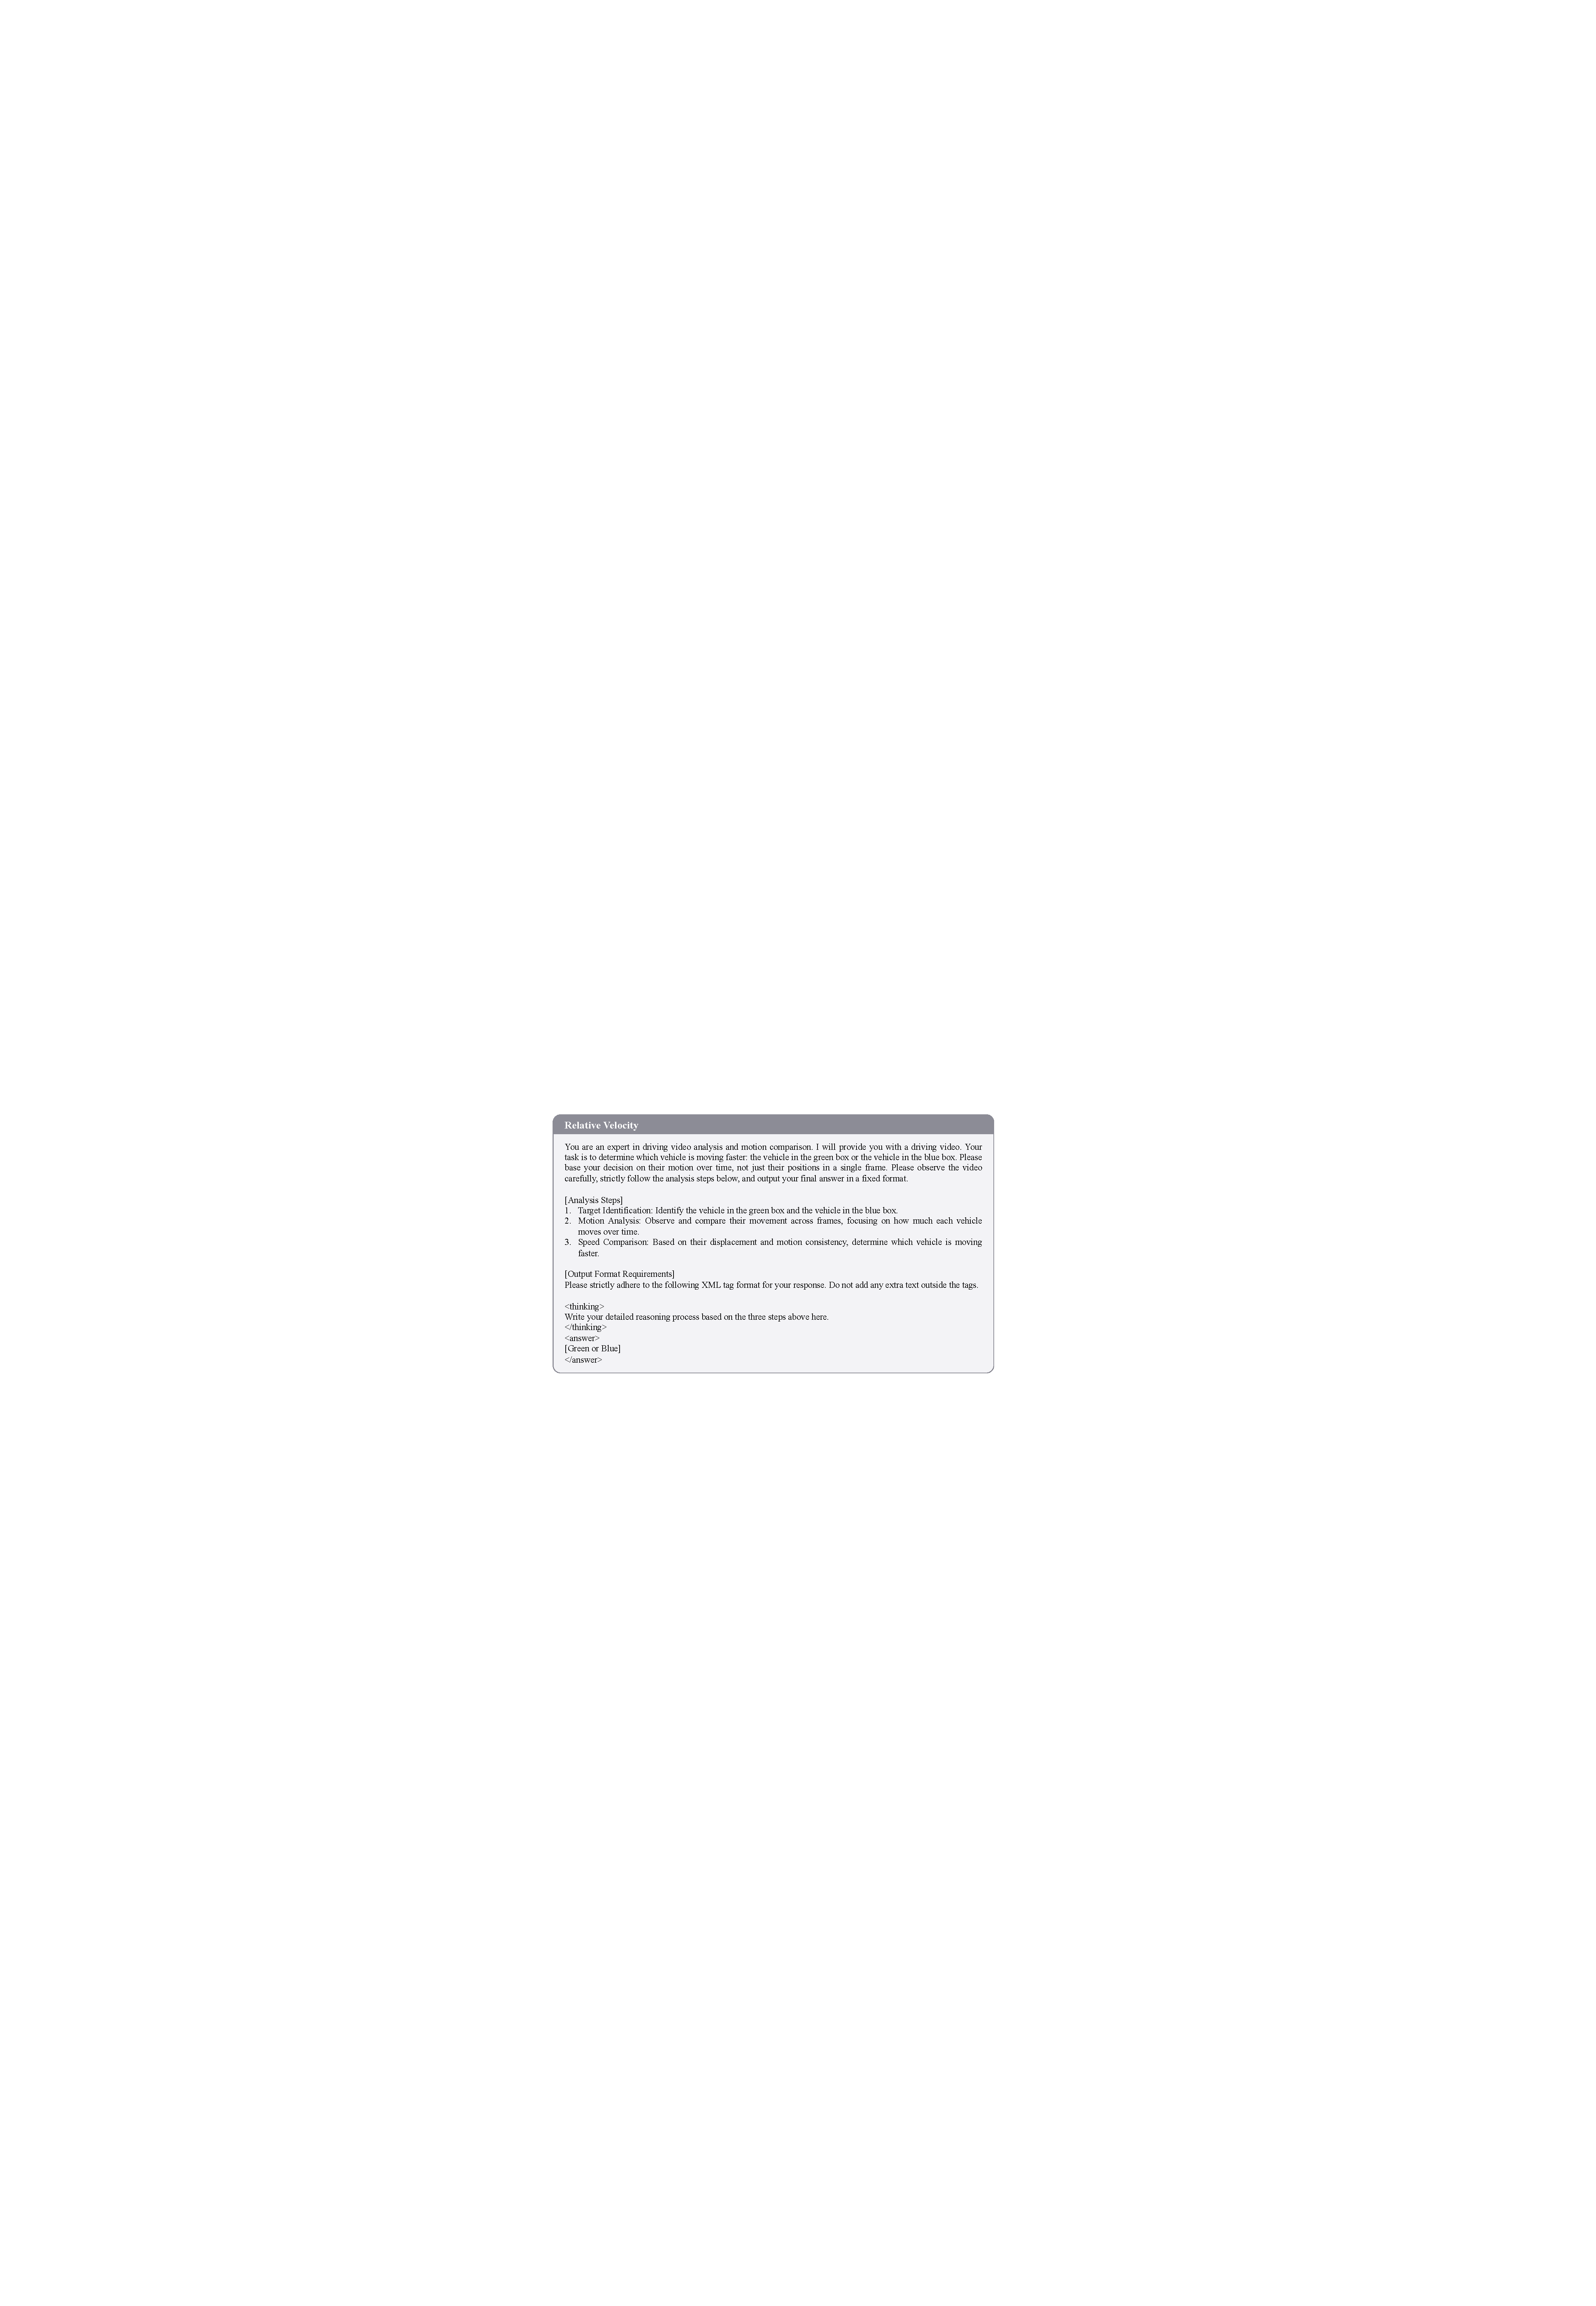
\includegraphics[width=0.95\linewidth]{fig/fig_7.pdf}
  \caption{\textbf{Manual CoT prompt template for Relative Velocity.}}
  \label{fig:7}
\end{figure}

\begin{figure}[p]
  \centering
  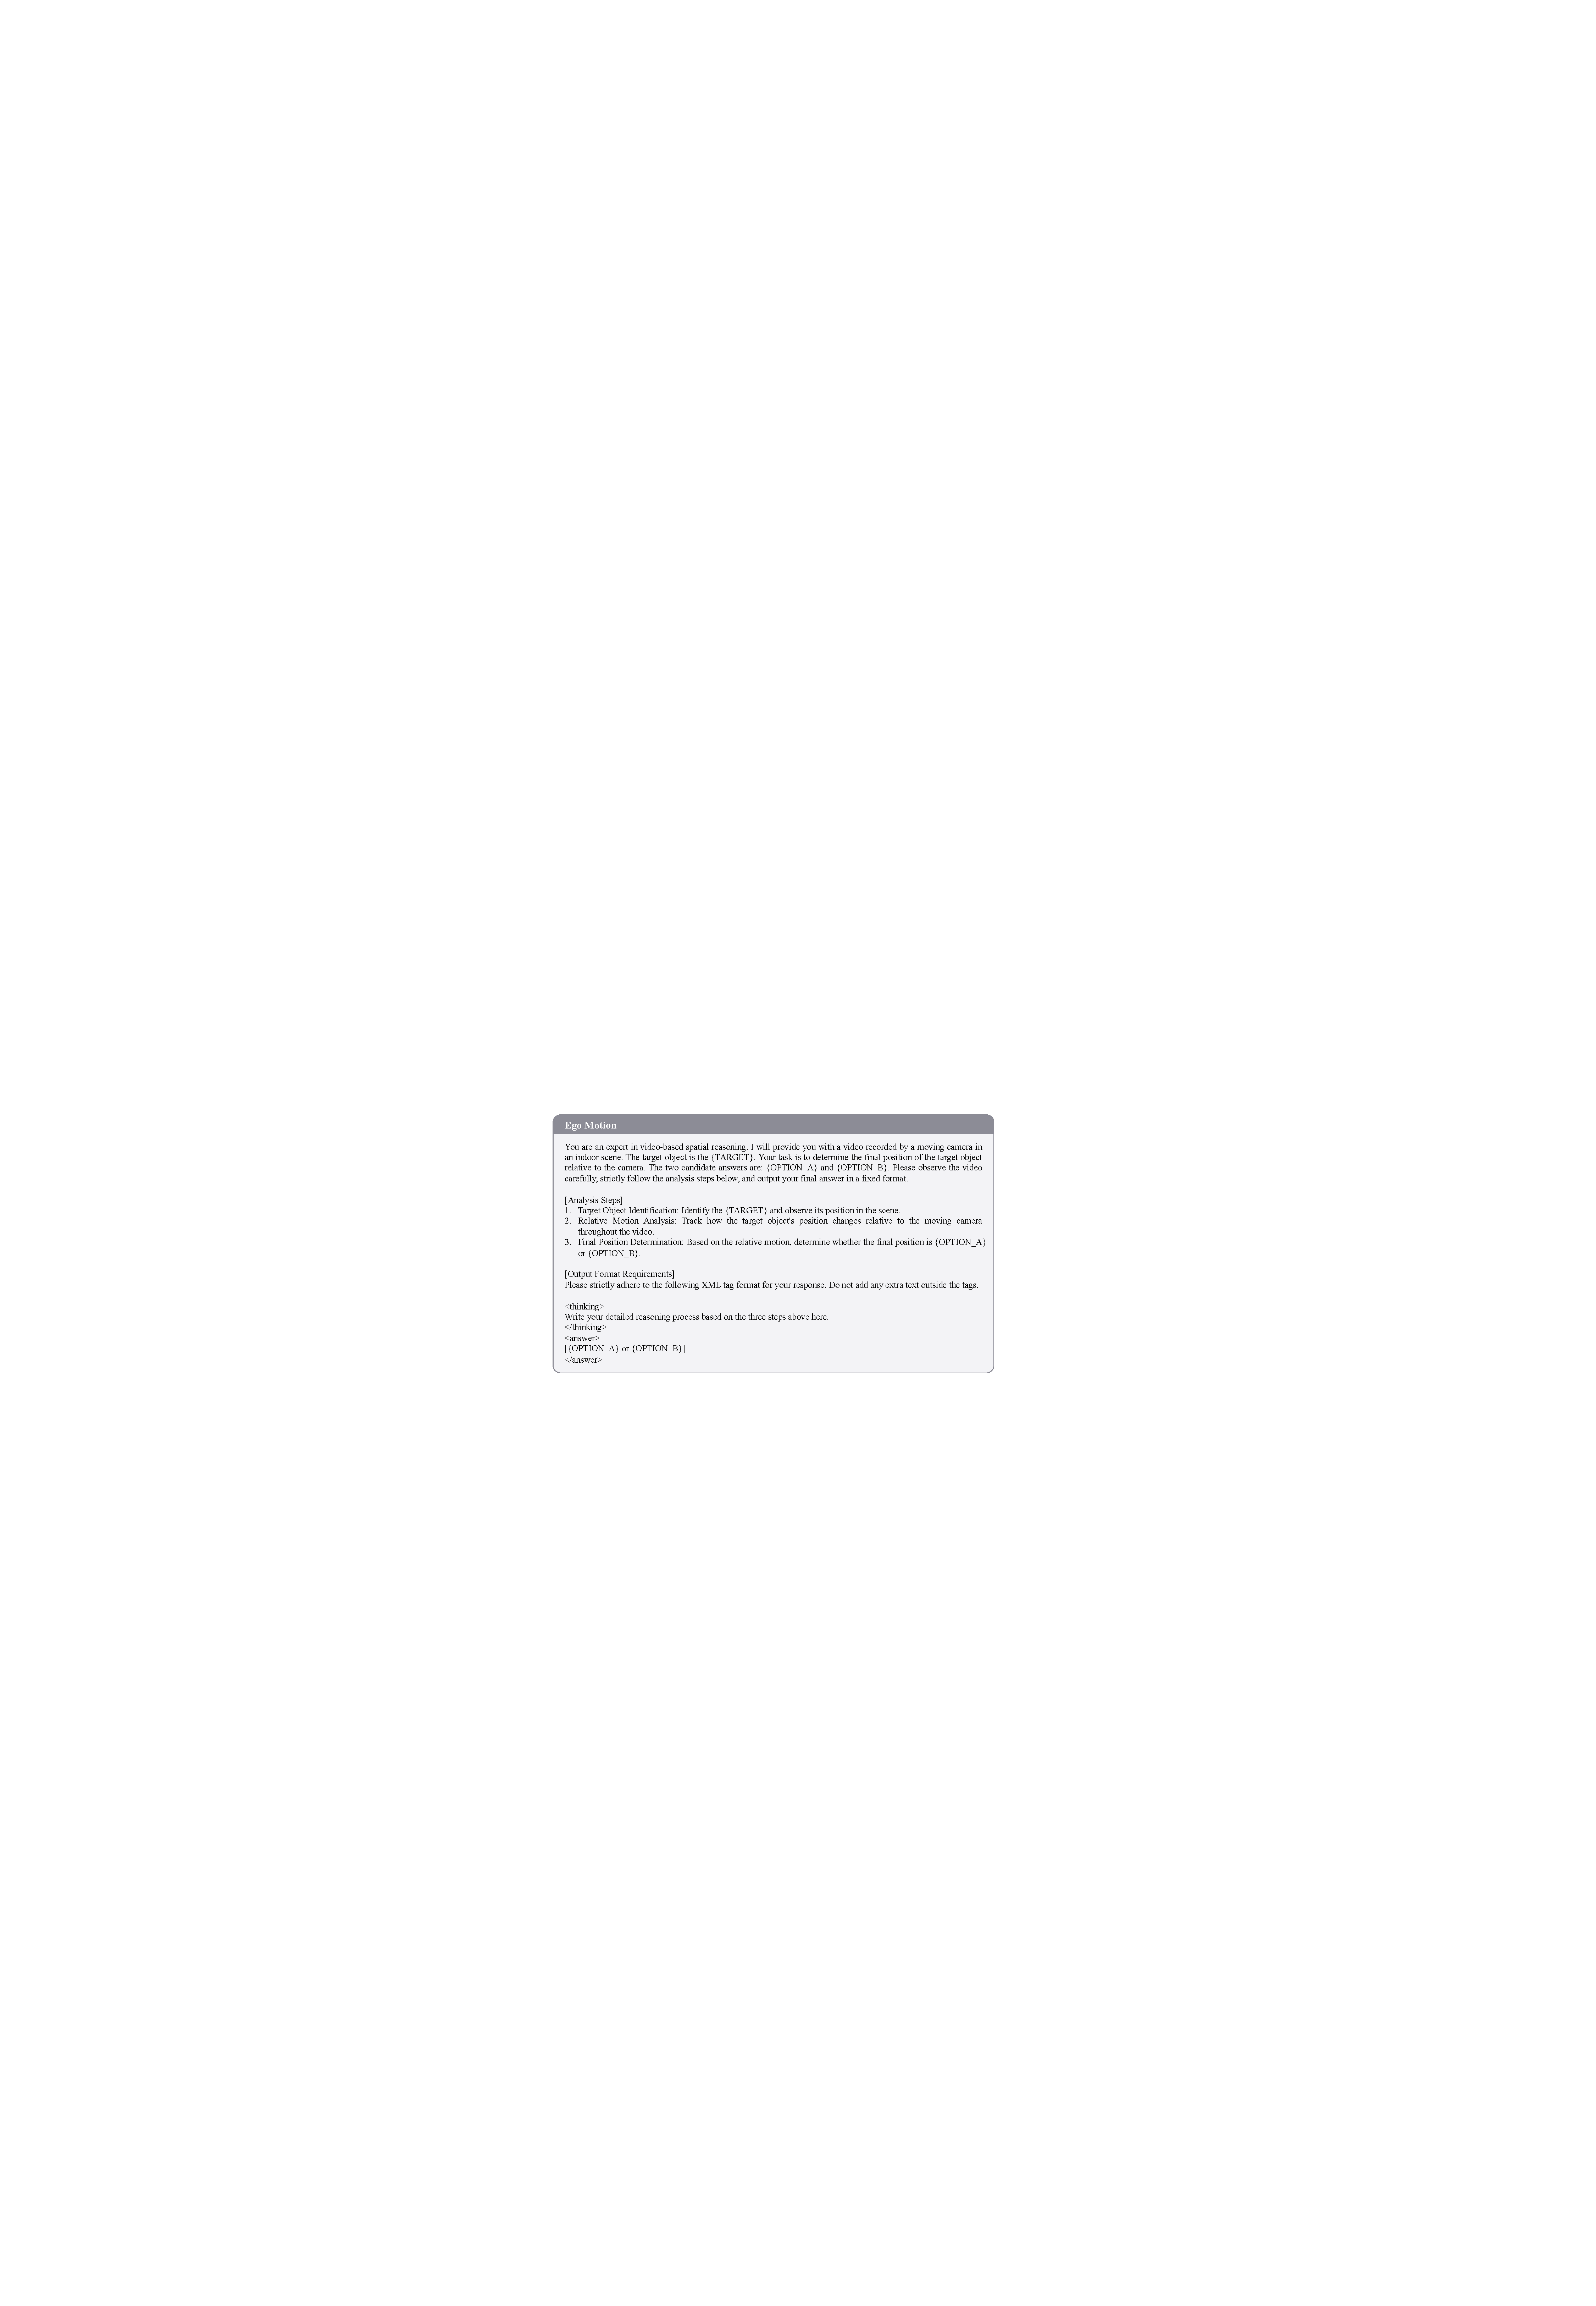
\includegraphics[width=0.95\linewidth]{fig/fig_8.pdf}
  \caption{\textbf{Manual CoT prompt template for Ego Motion.}}
  \label{fig:8}
\end{figure}

\begin{figure}[p]
  \centering
  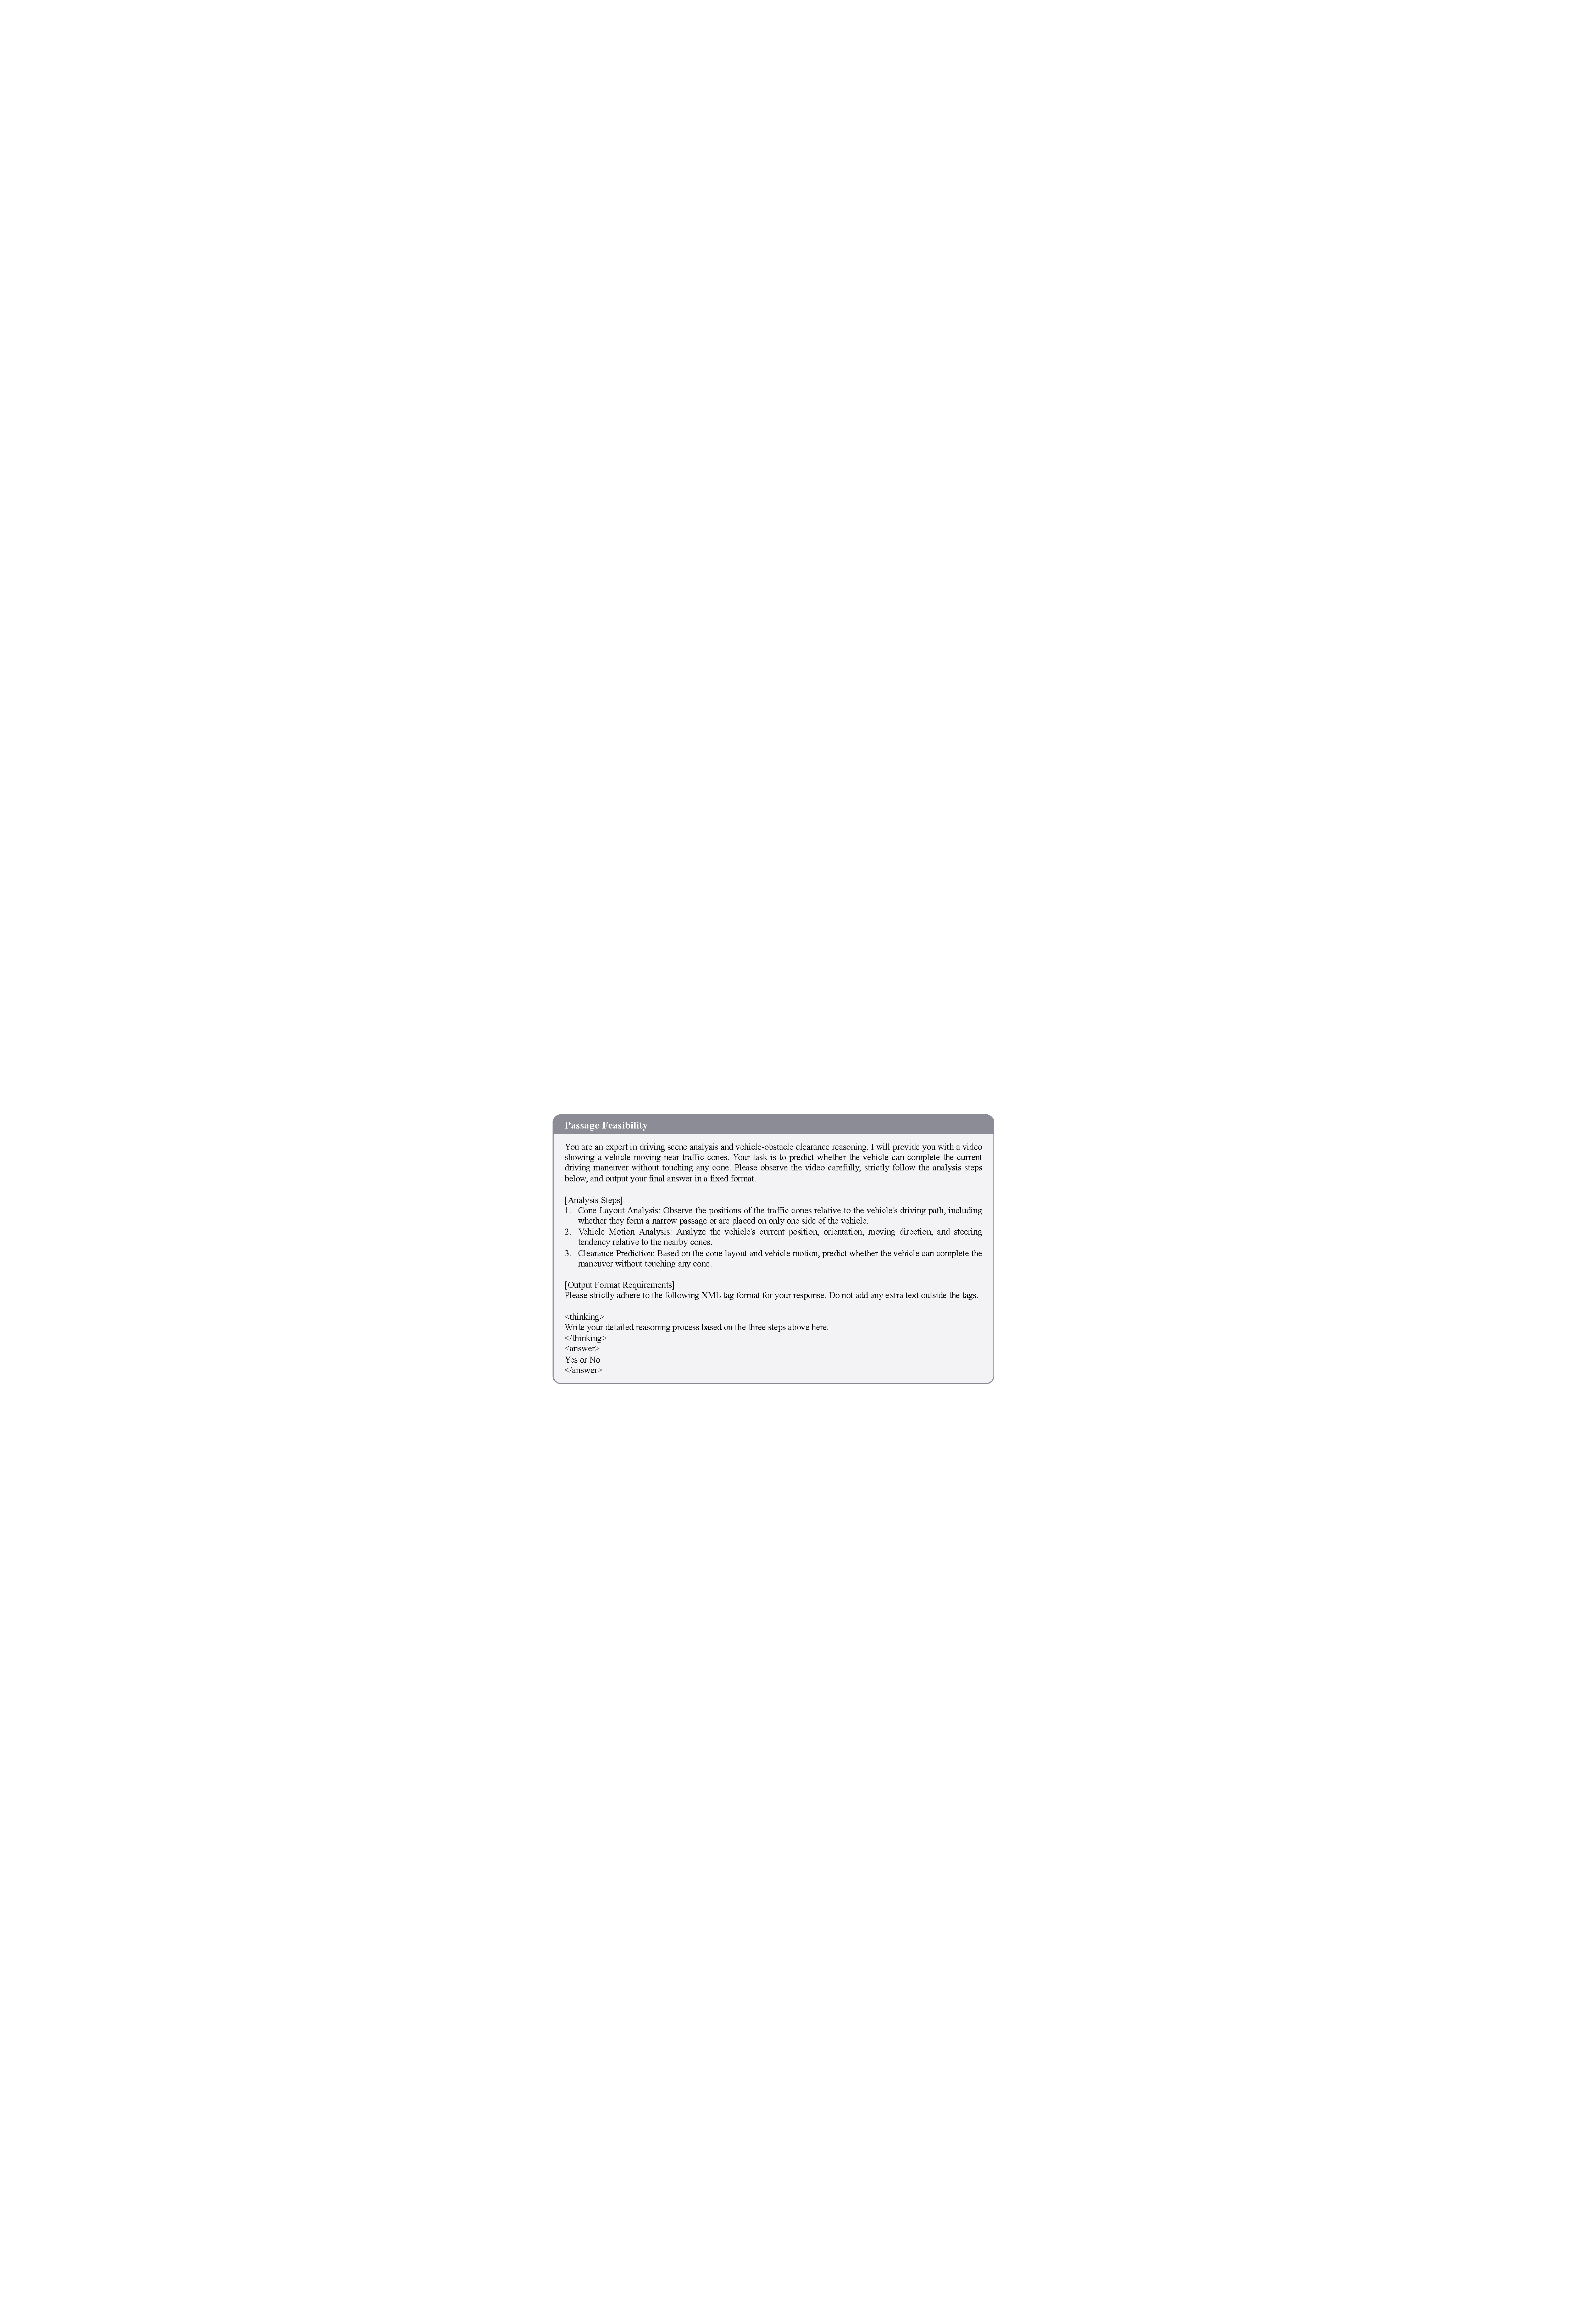
\includegraphics[width=0.95\linewidth]{fig/fig_9.pdf}
  \caption{\textbf{Manual CoT prompt template for Passage Feasibility.}}
  \label{fig:9}
\end{figure}

\begin{figure}[p]
  \centering
  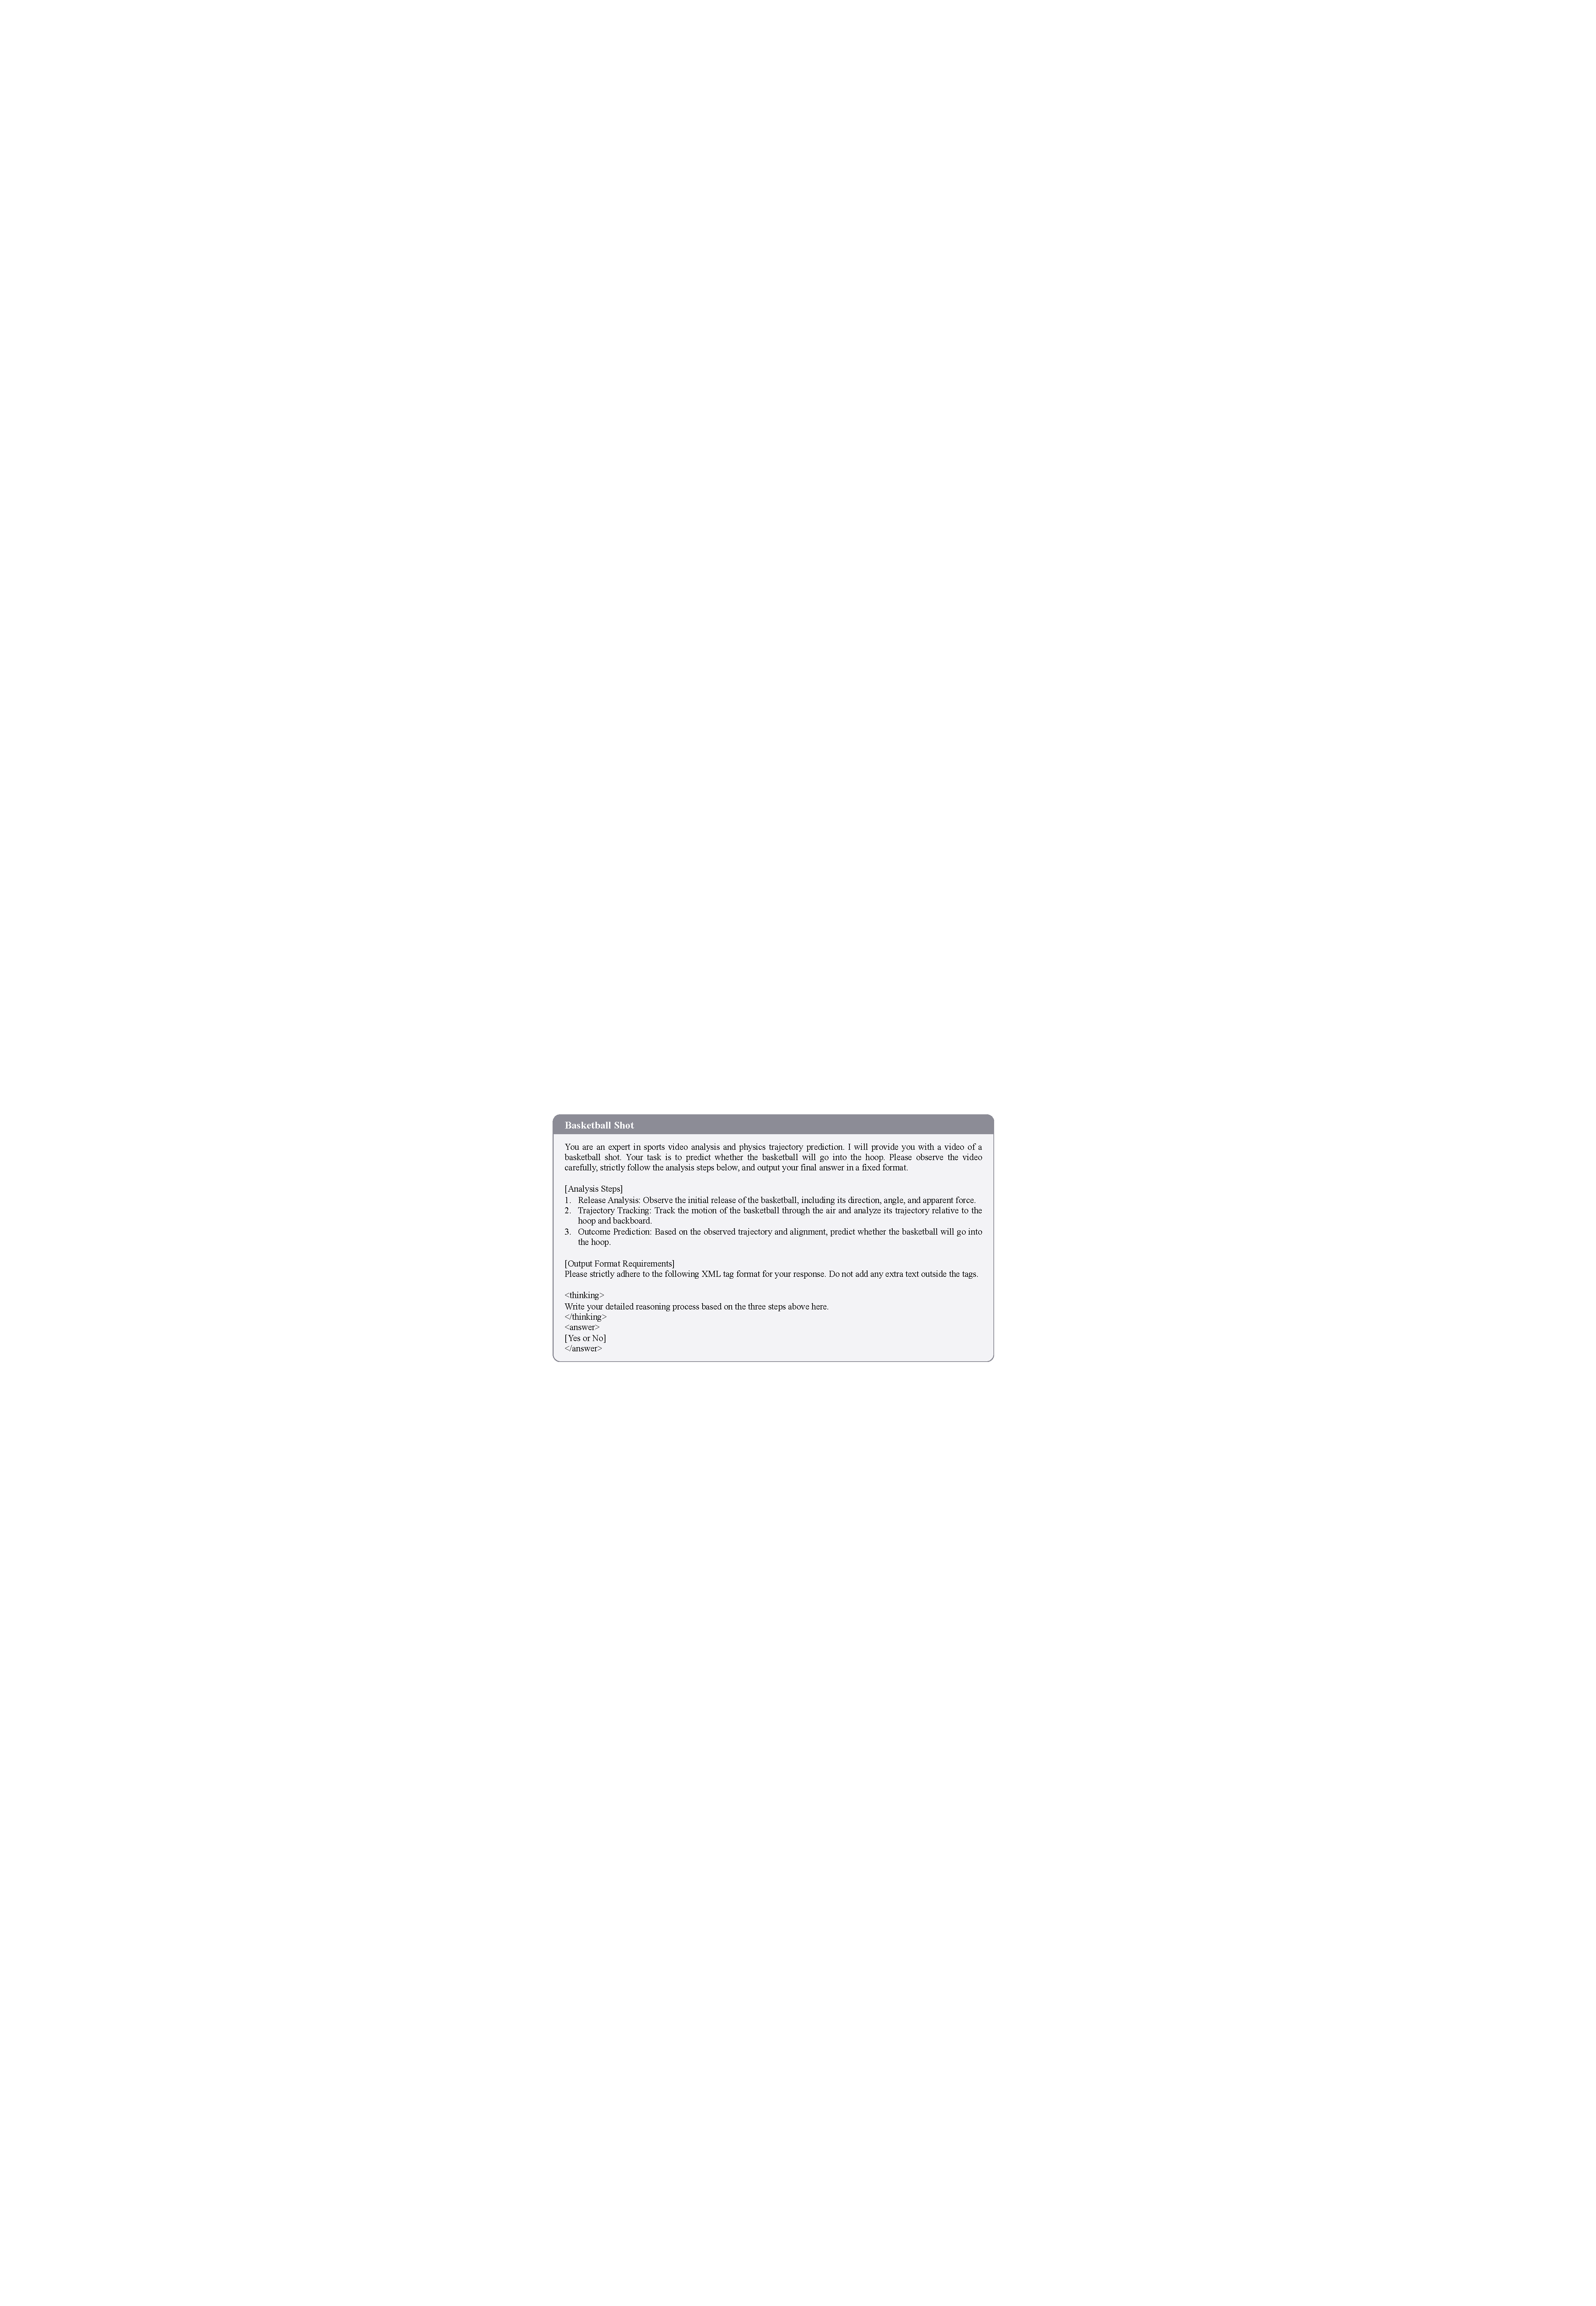
\includegraphics[width=0.95\linewidth]{fig/fig_10.pdf}
  \caption{\textbf{Manual CoT prompt template for Basketball Shot.}}
  \label{fig:10}
\end{figure}

\begin{figure}[p]
  \centering
  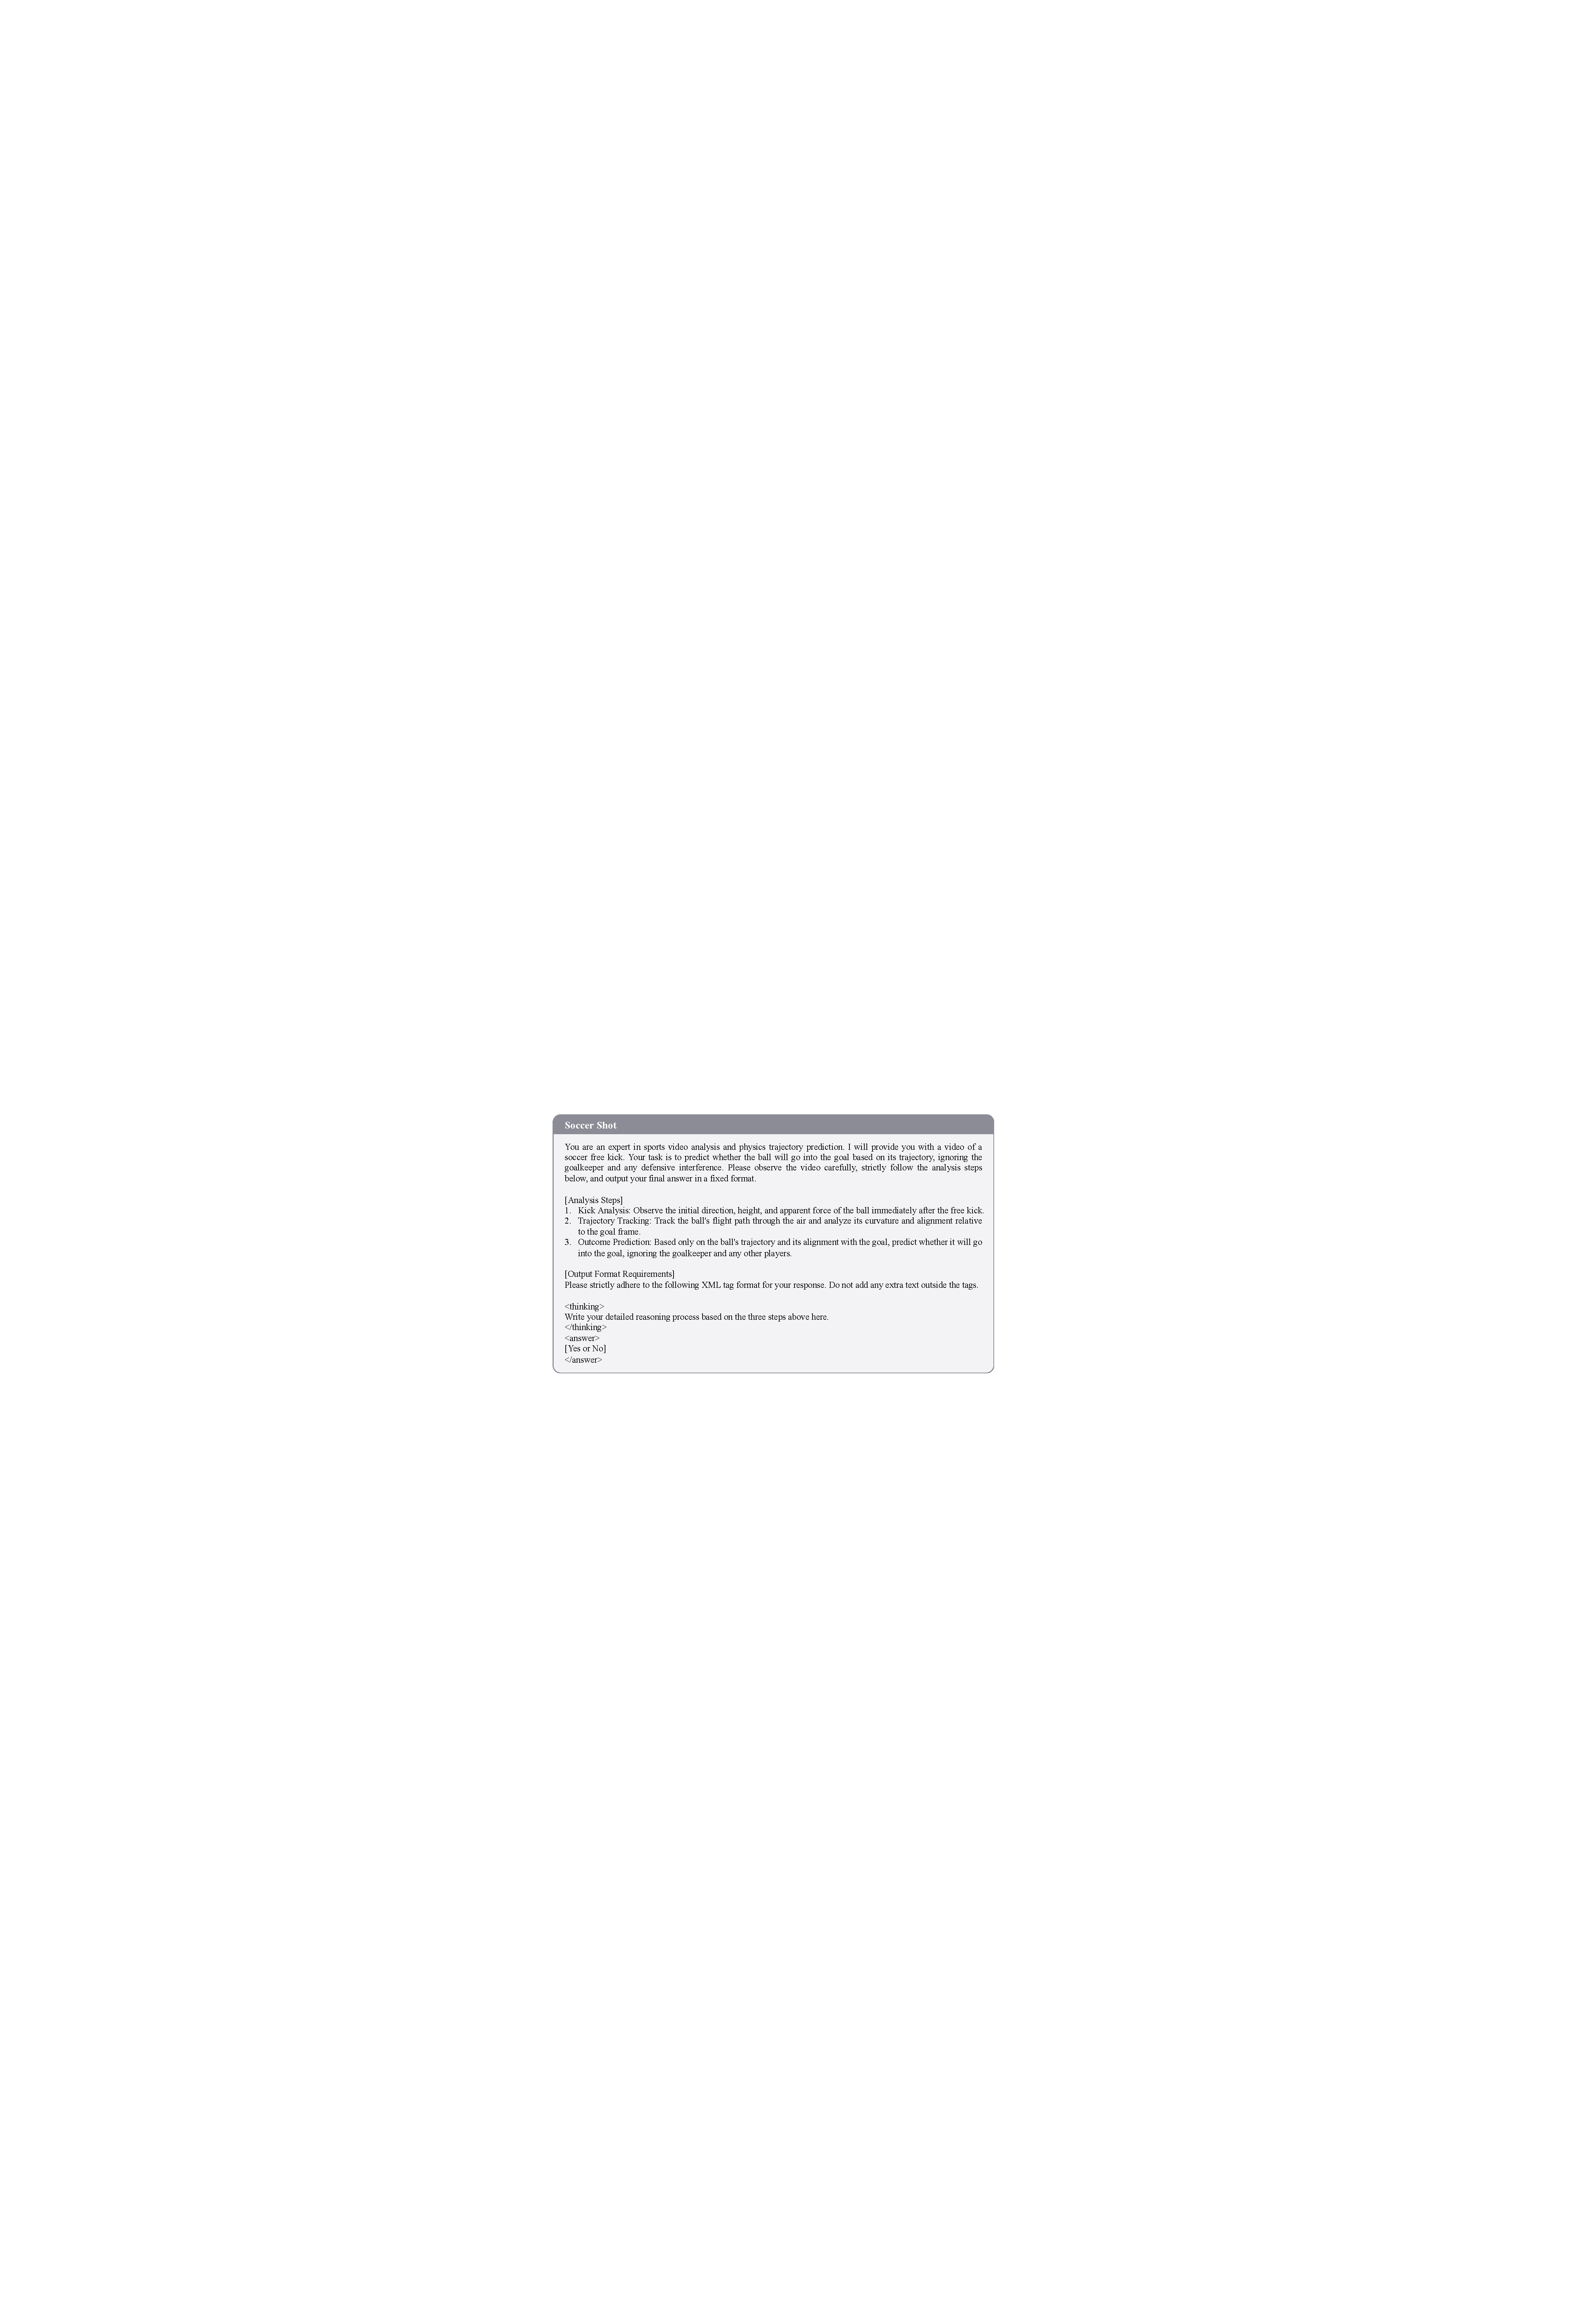
\includegraphics[width=0.95\linewidth]{fig/fig_11.pdf}
  \caption{\textbf{Manual CoT prompt template for Soccer Shot.}}
  \label{fig:11}
\end{figure}

\begin{figure}[p]
  \centering
  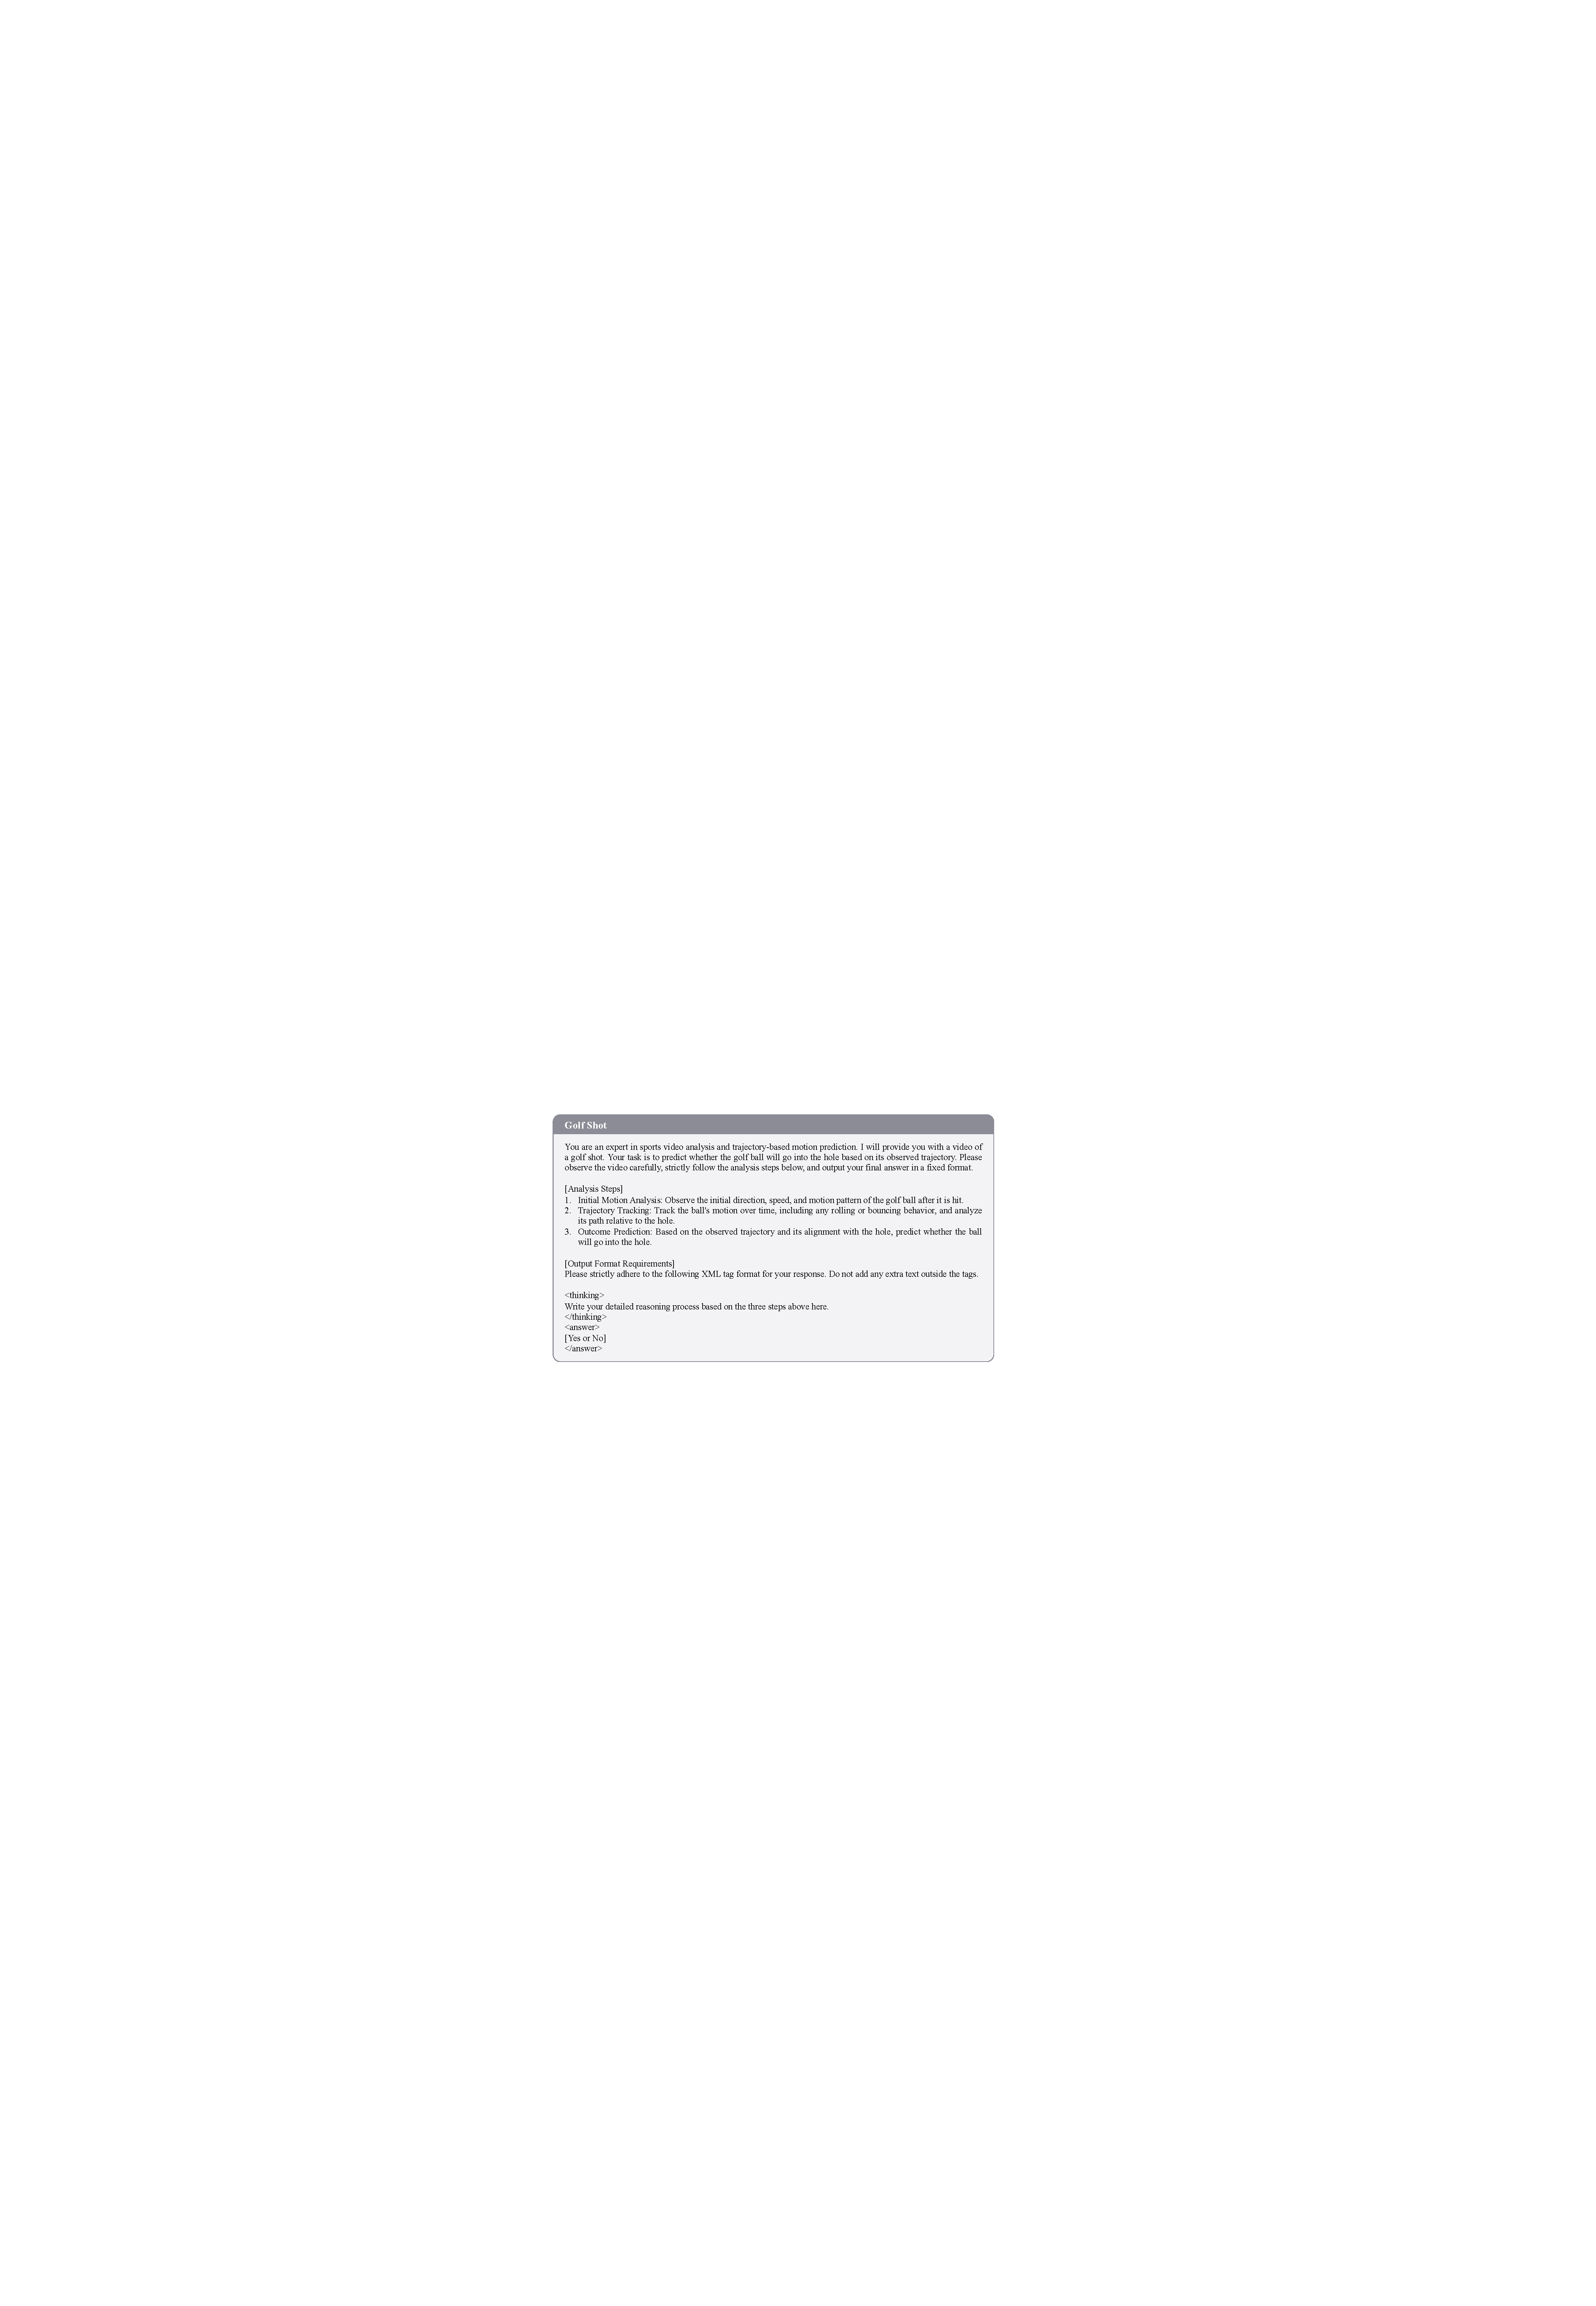
\includegraphics[width=0.95\linewidth]{fig/fig_12.pdf}
  \caption{\textbf{Manual CoT prompt template for Golf Shot.}}
  \label{fig:12}
\end{figure}

\begin{figure}[p]
  \centering
  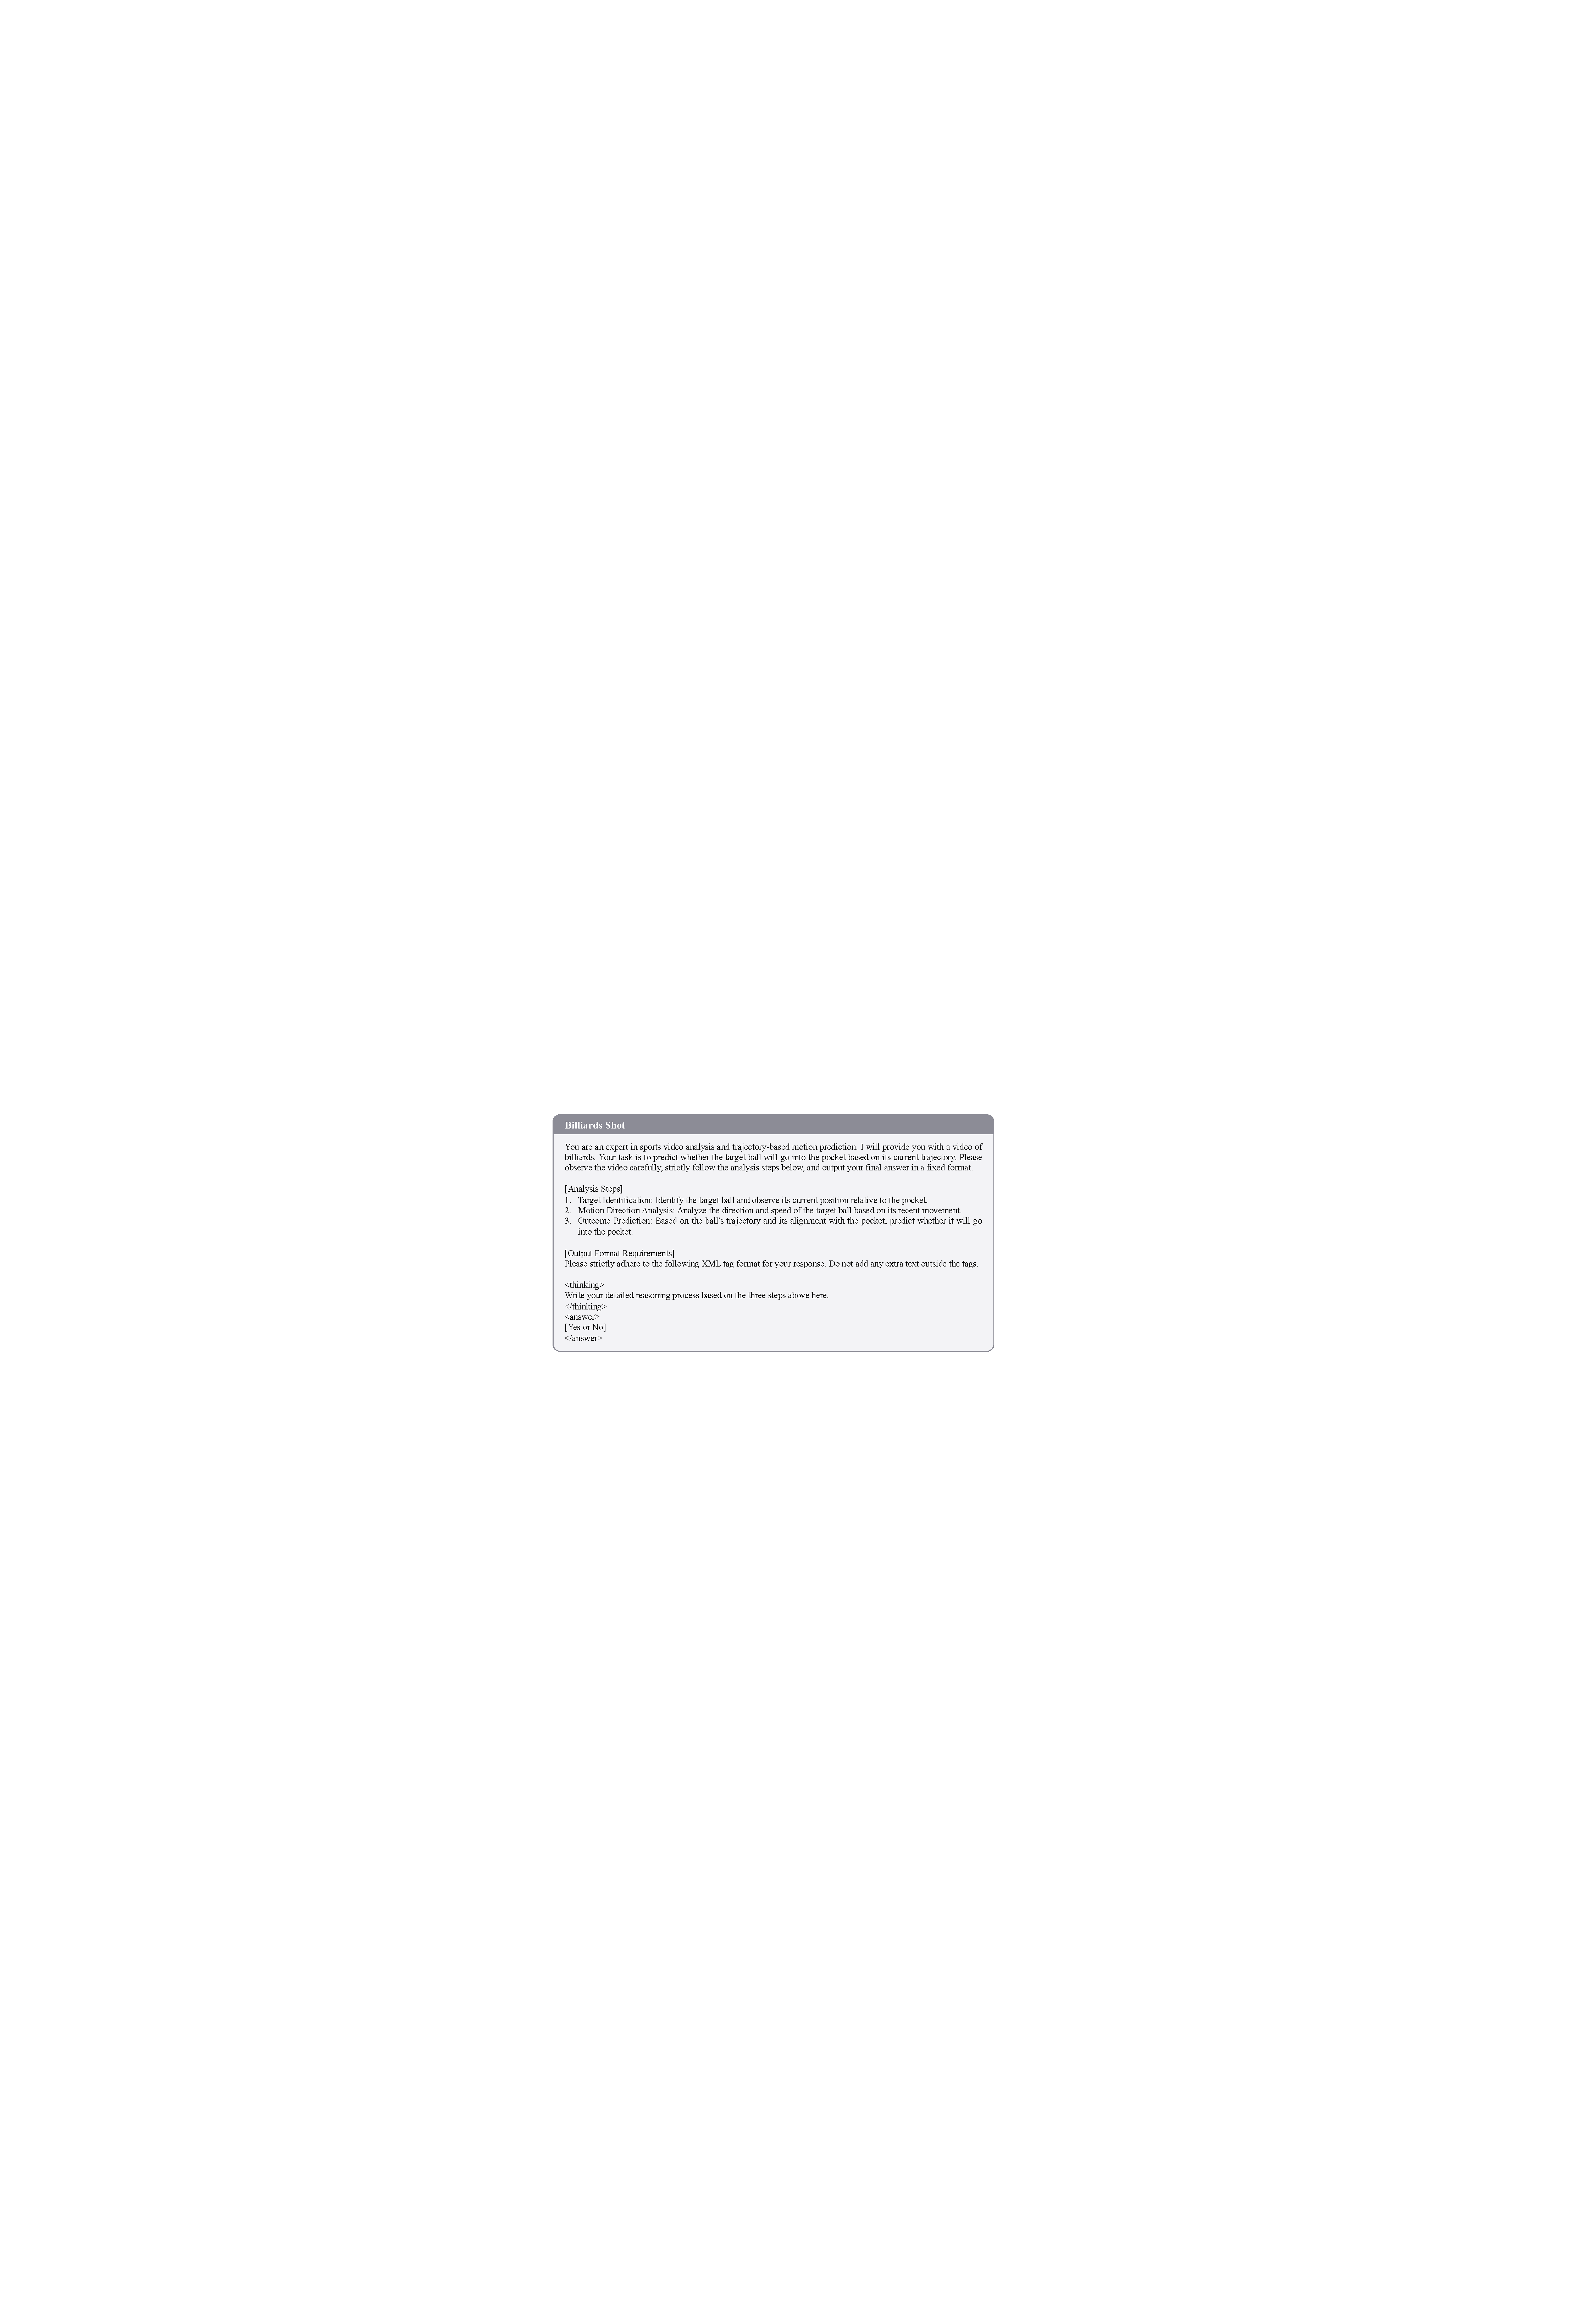
\includegraphics[width=0.95\linewidth]{fig/fig_13.pdf}
  \caption{\textbf{Manual CoT prompt template for Billiards Shot.}}
  \label{fig:13}
\end{figure}

\begin{figure}[p]
  \centering
  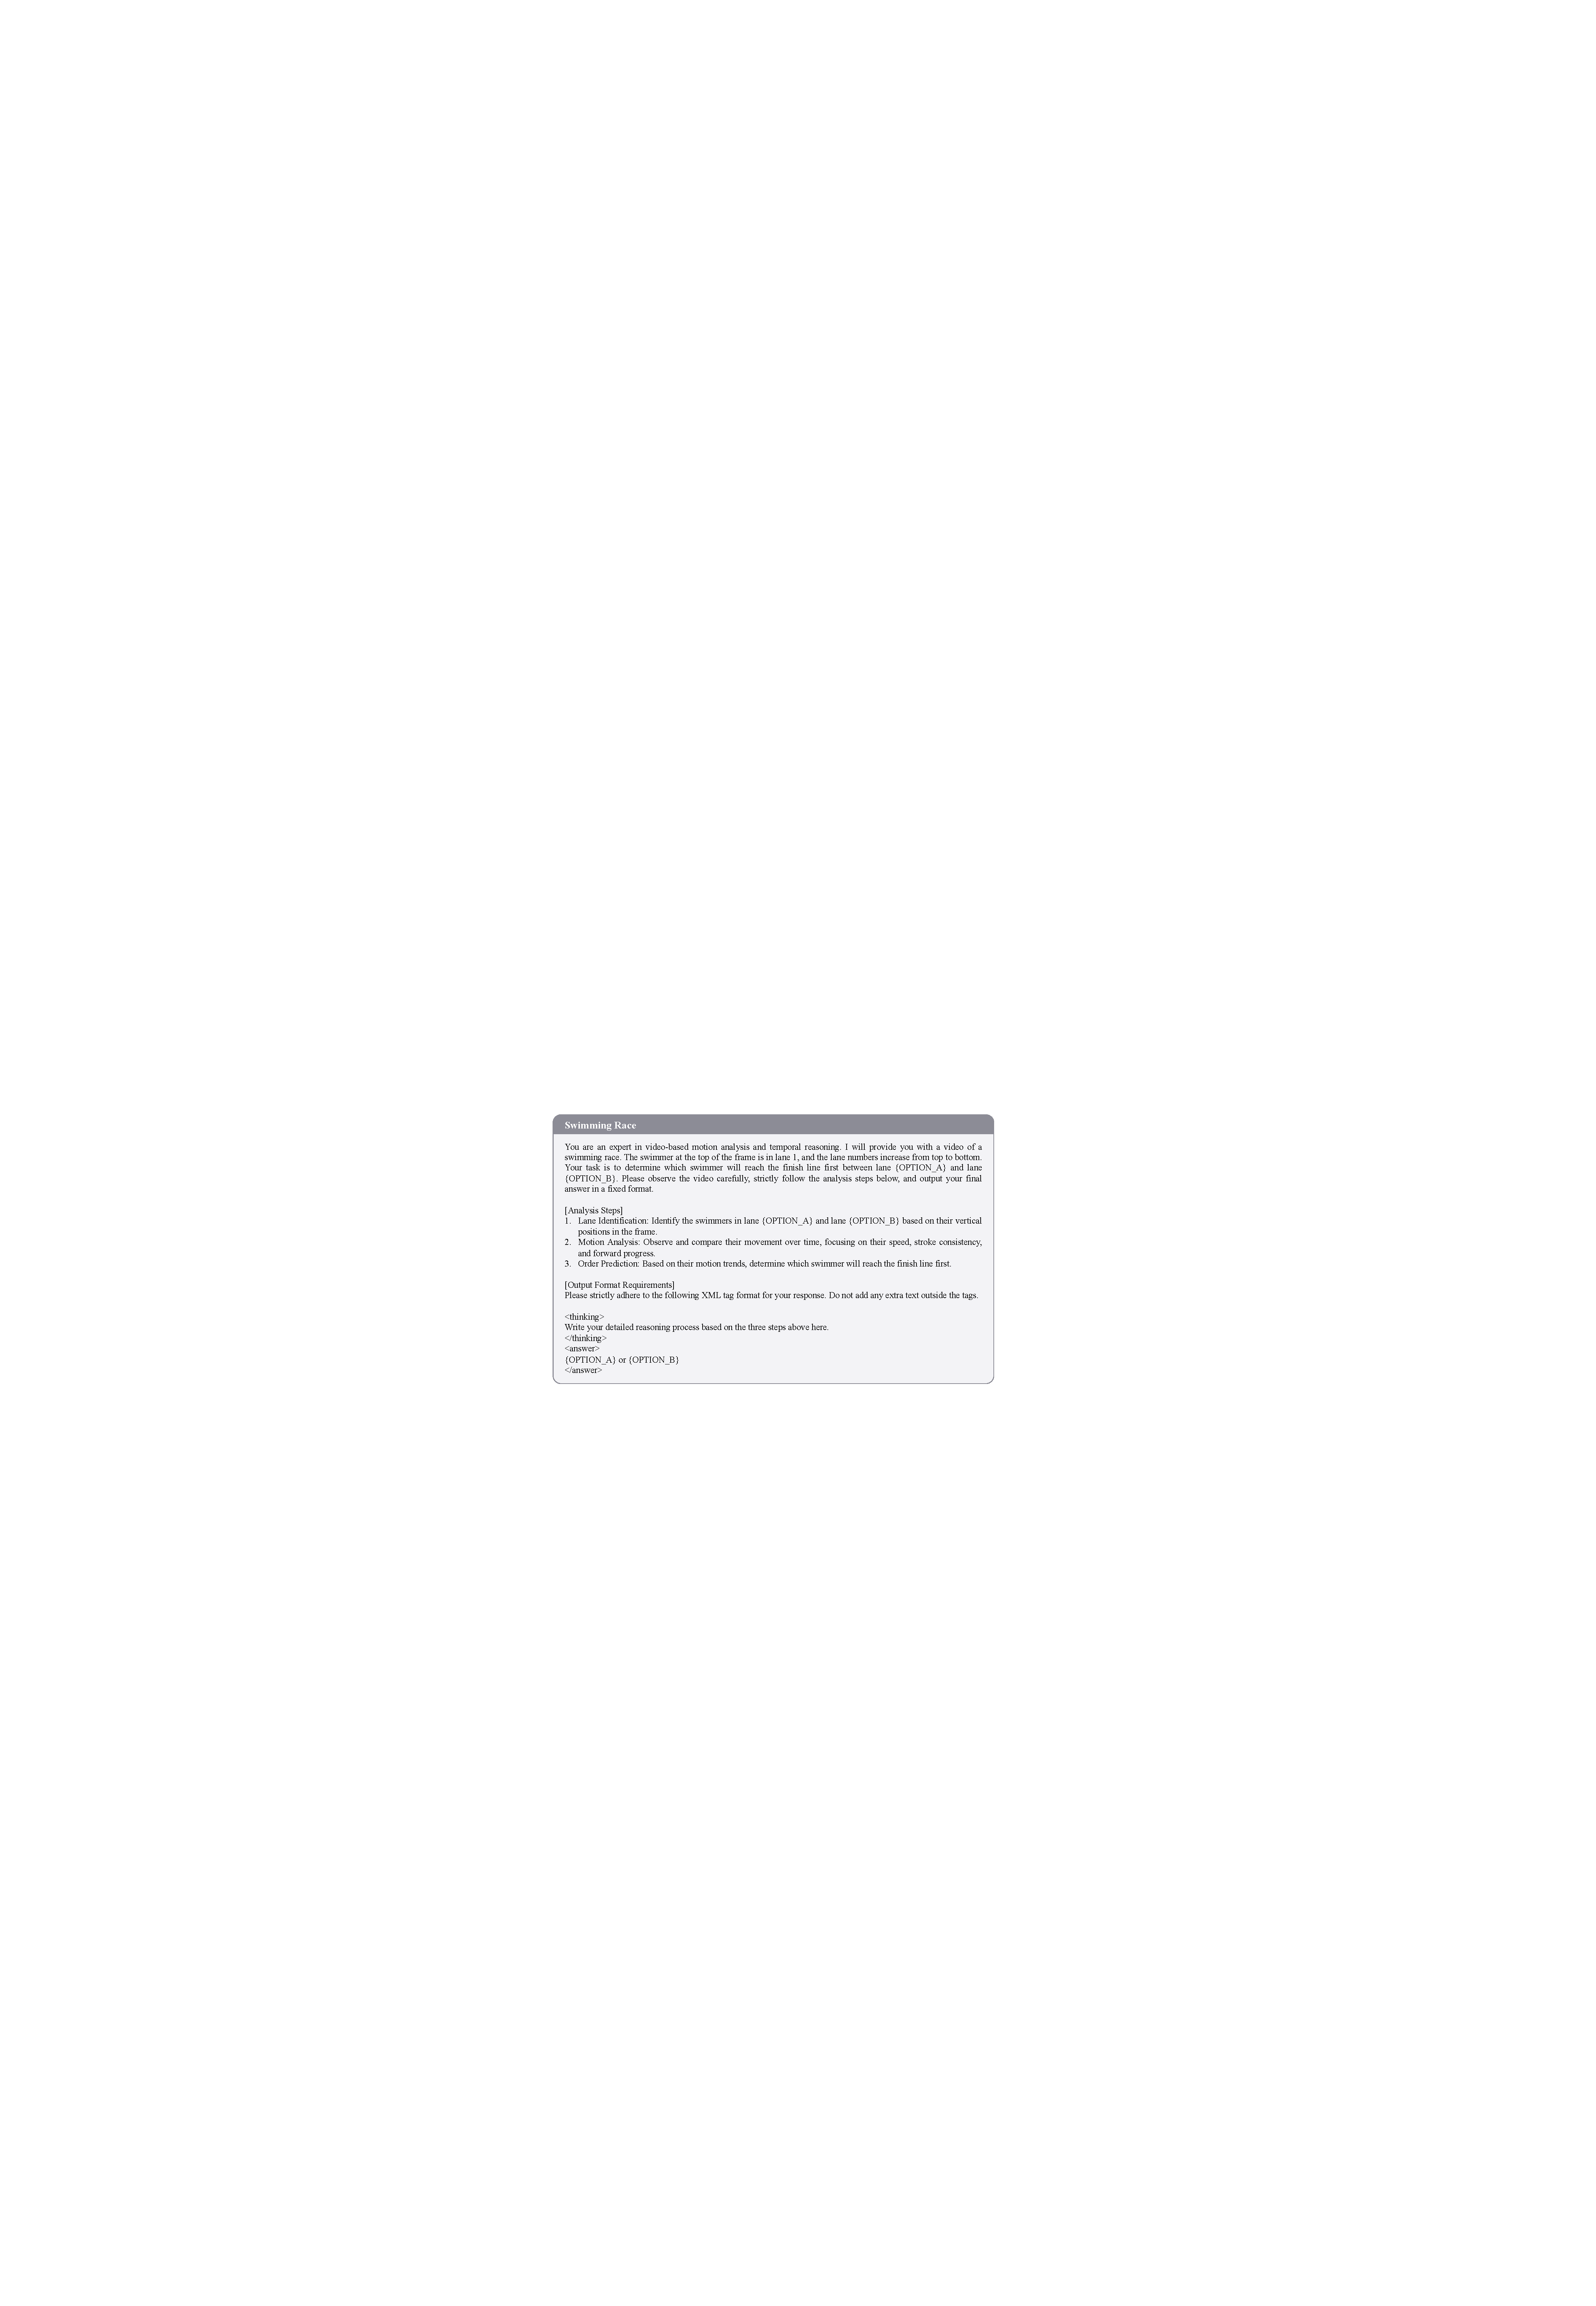
\includegraphics[width=0.95\linewidth]{fig/fig_14.pdf}
  \caption{\textbf{Manual CoT prompt template for Swimming Race.}}
  \label{fig:14}
\end{figure}

\begin{figure}[p]
  \centering
  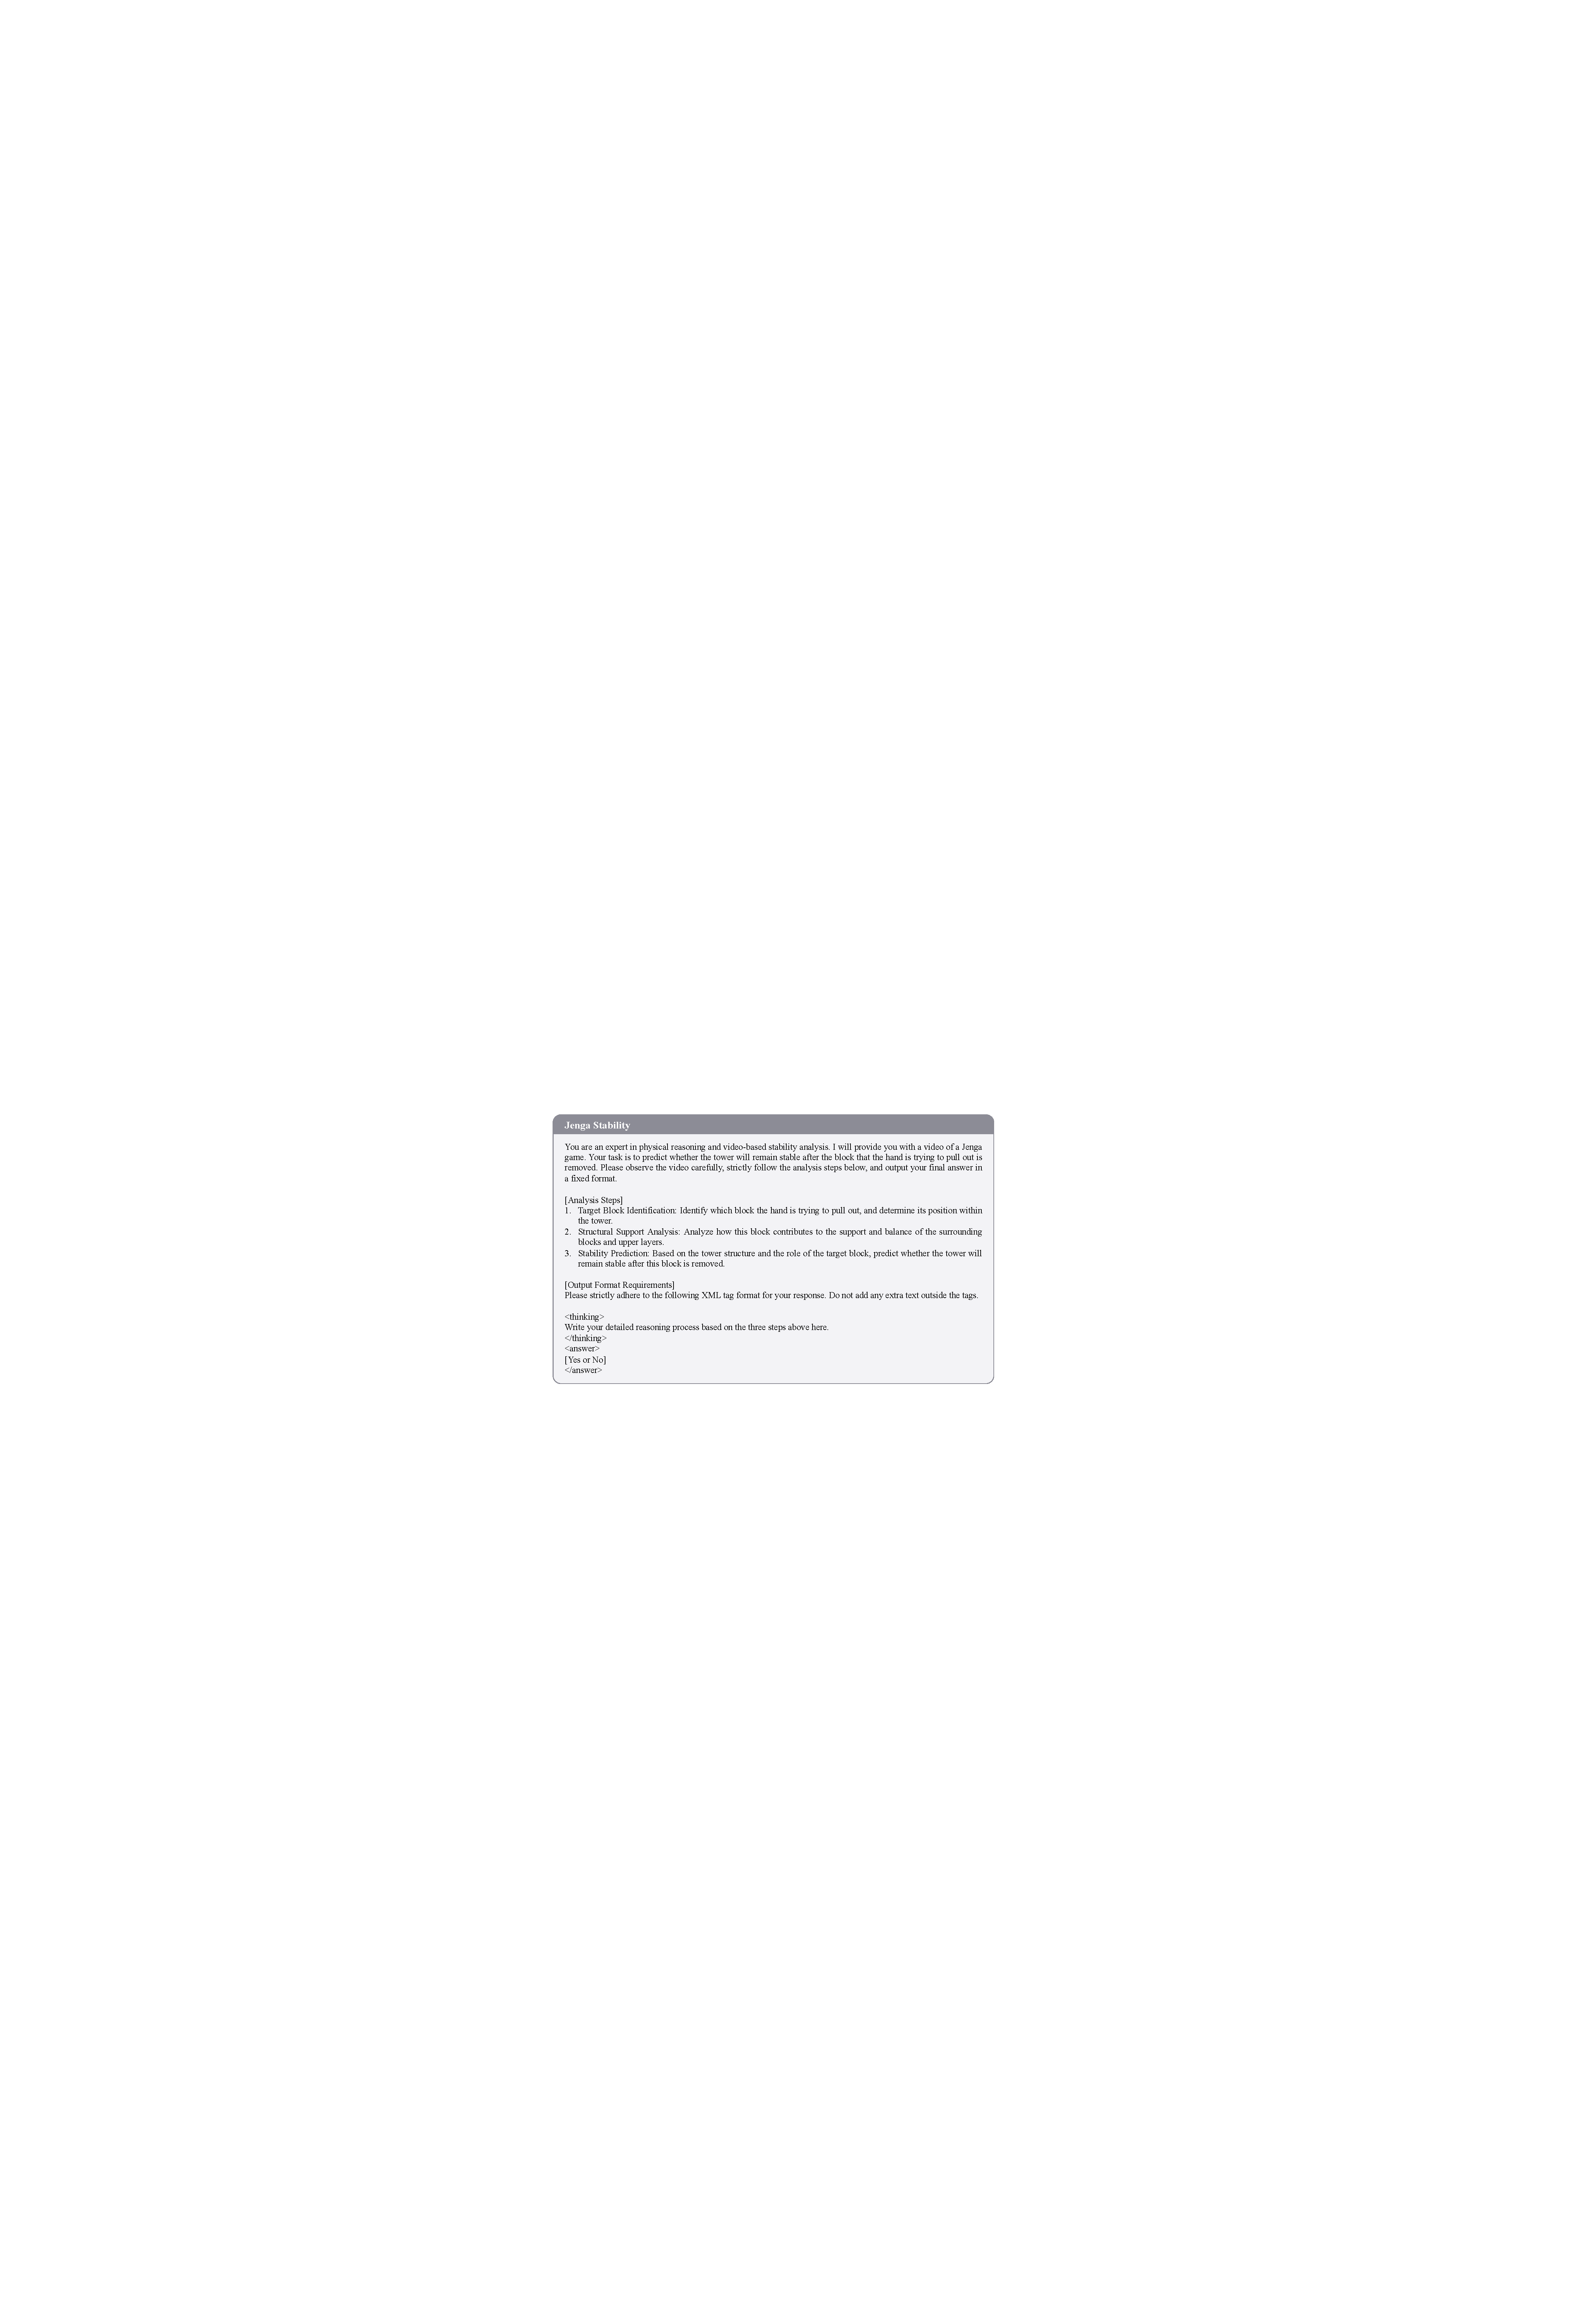
\includegraphics[width=0.95\linewidth]{fig/fig_15.pdf}
  \caption{\textbf{Manual CoT prompt template for Jenga Stability.}}
  \label{fig:15}
\end{figure}

\begin{figure}[p]
  \centering
  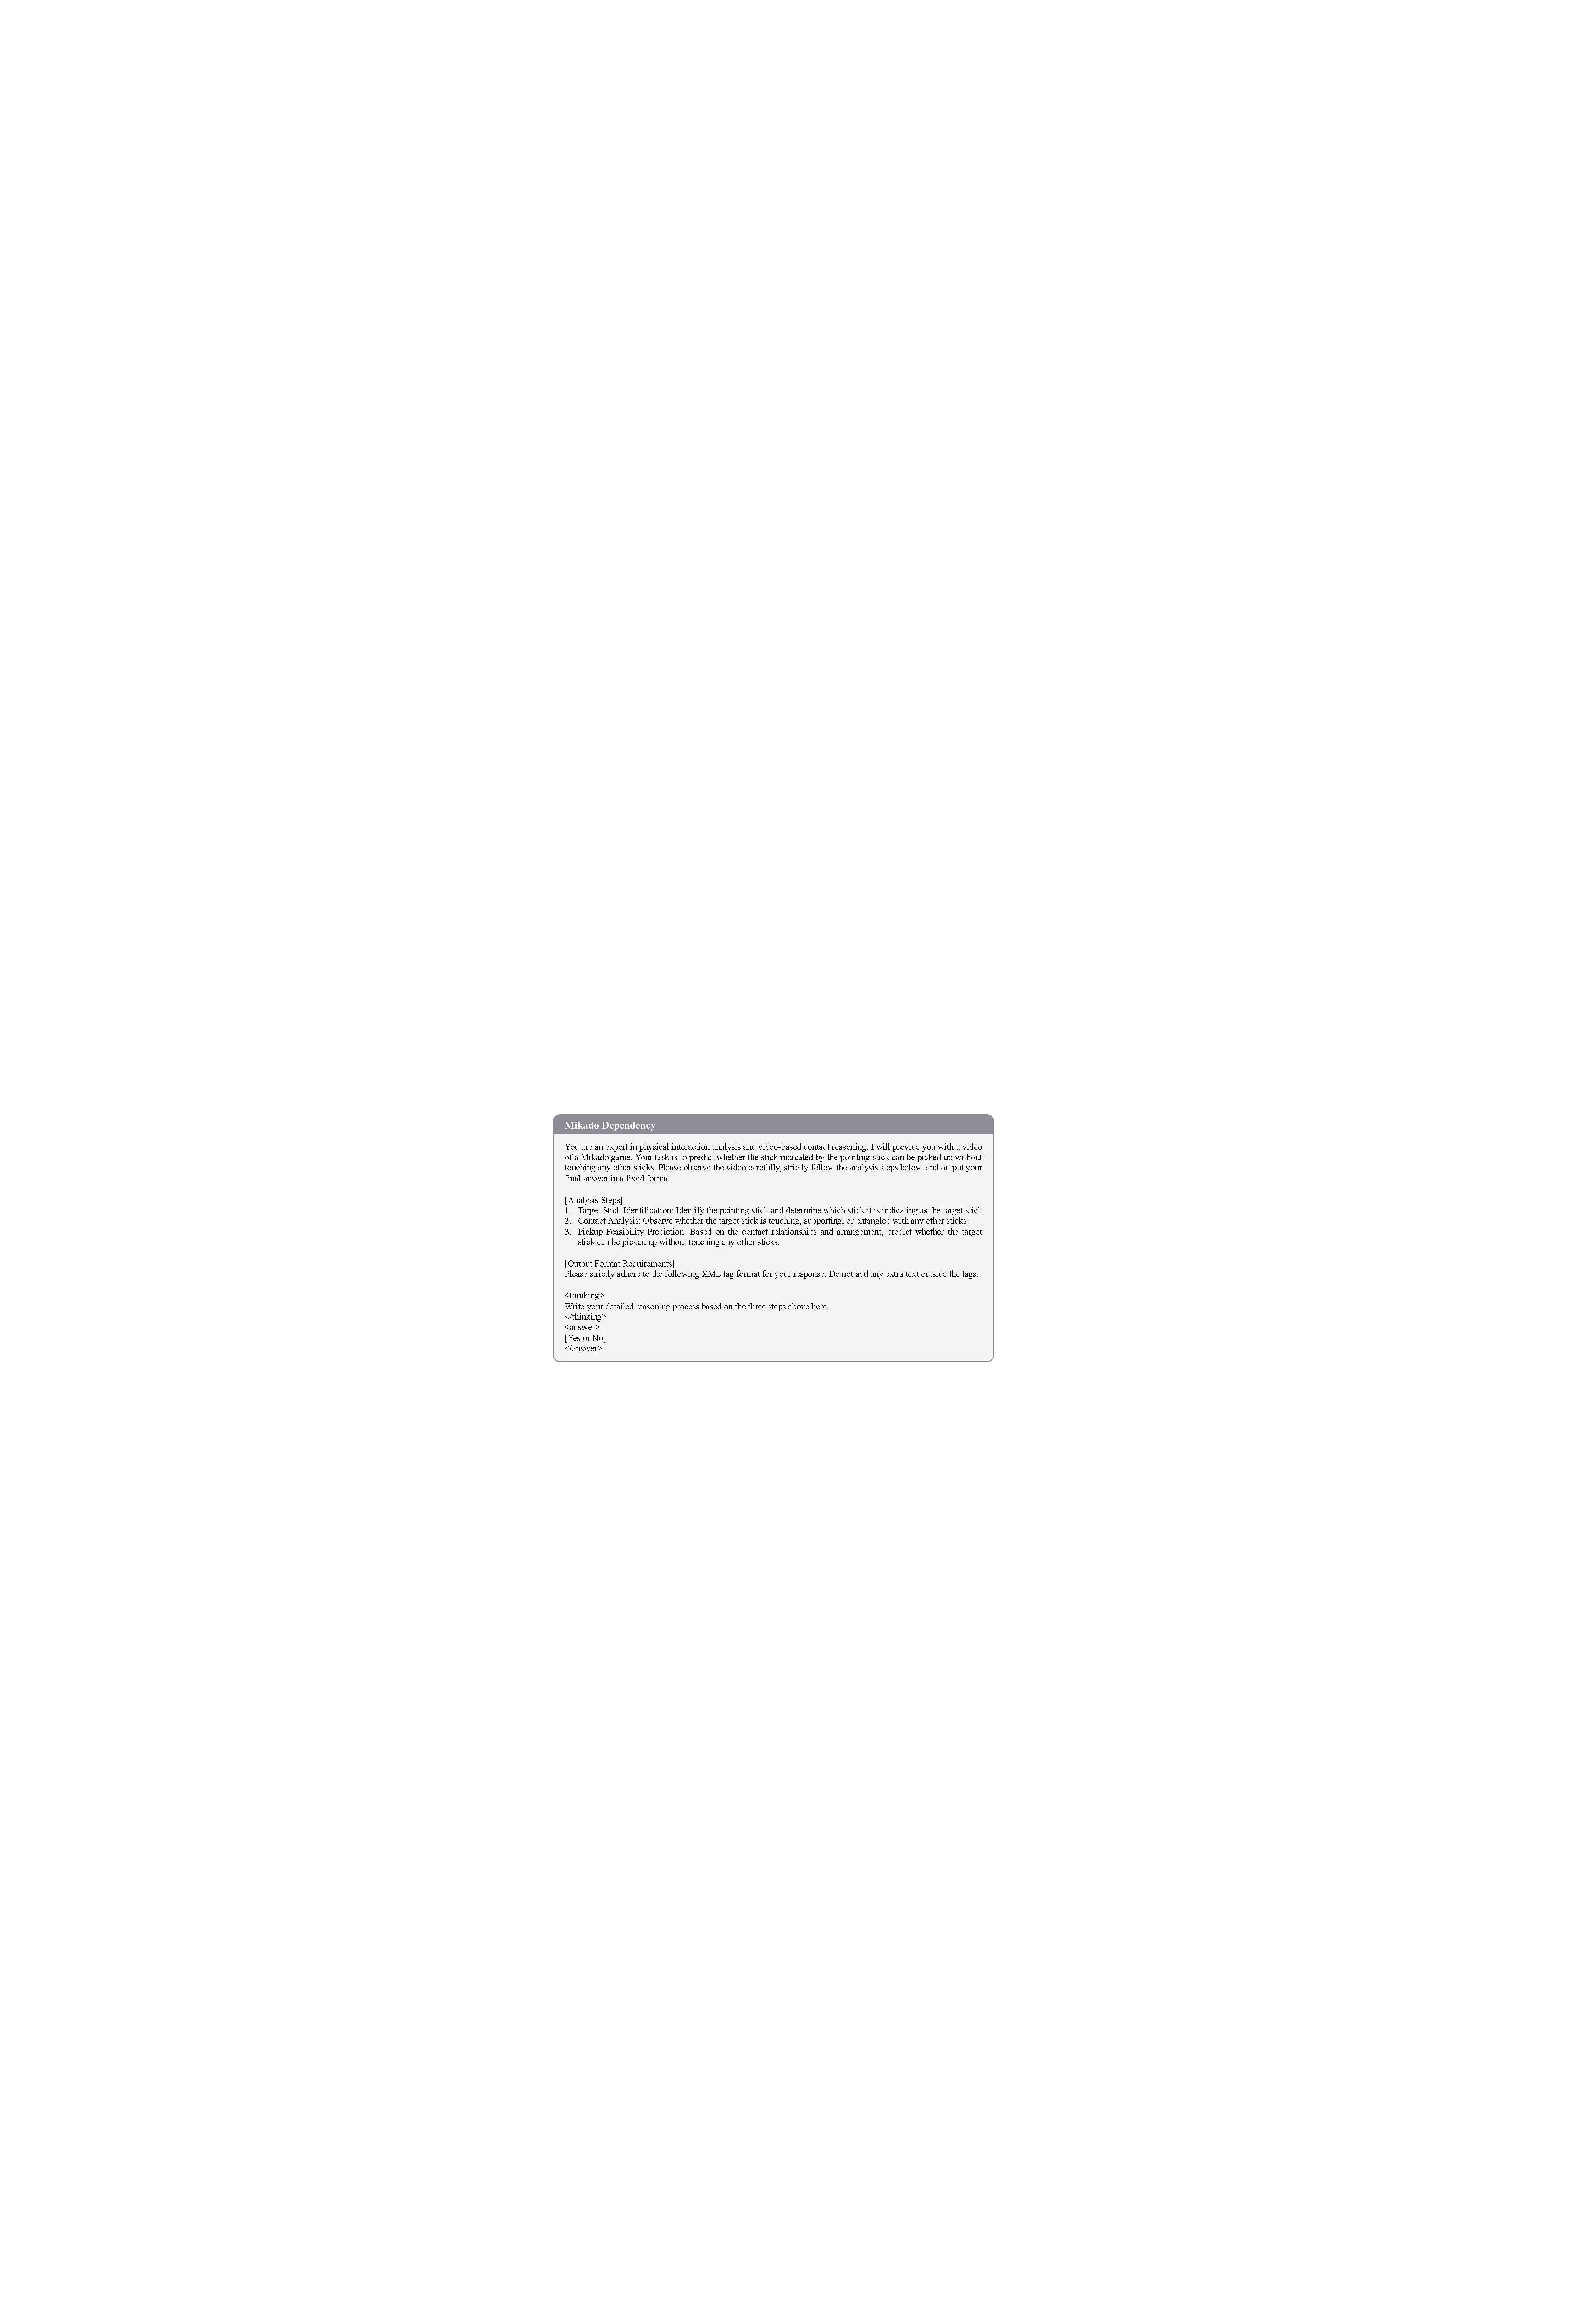
\includegraphics[width=0.95\linewidth]{fig/fig_16.pdf}
  \caption{\textbf{Manual CoT prompt template for Mikado Dependency.}}
  \label{fig:16}
\end{figure}

\begin{figure}[p]
  \centering
  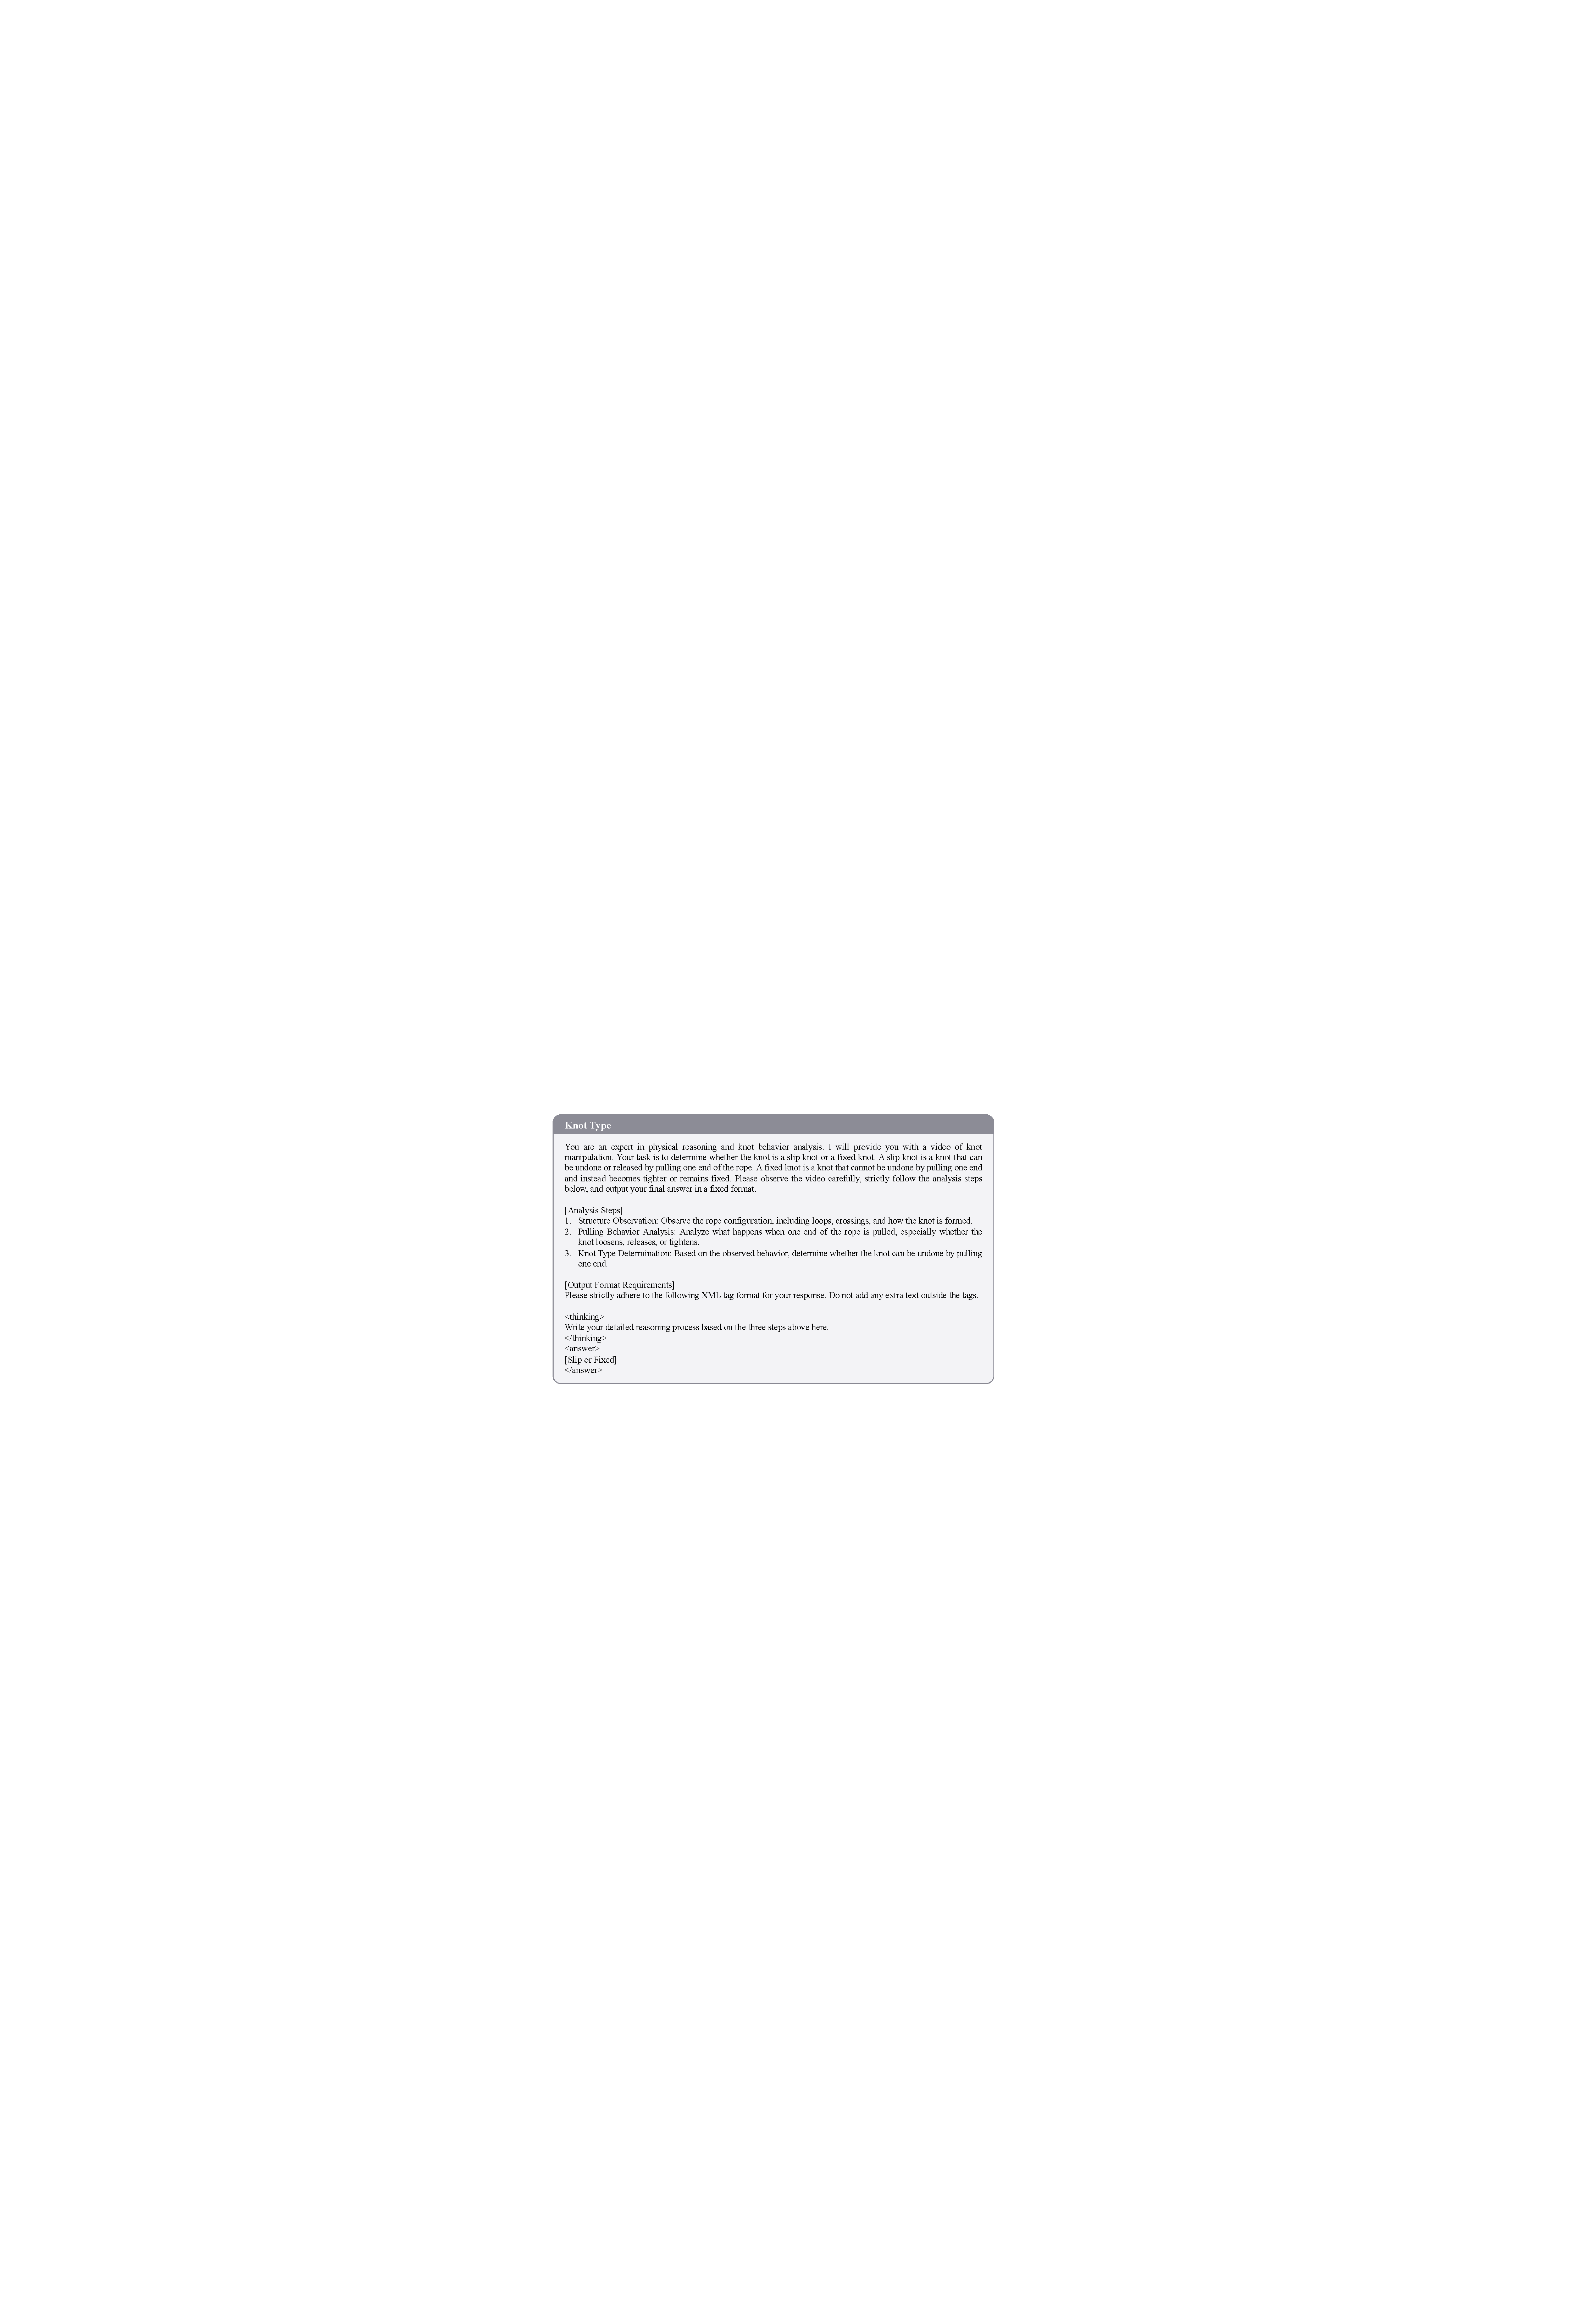
\includegraphics[width=0.95\linewidth]{fig/fig_17.pdf}
  \caption{\textbf{Manual CoT prompt template for Knot Type.}}
  \label{fig:17}
\end{figure}

\begin{figure}[p]
  \centering
  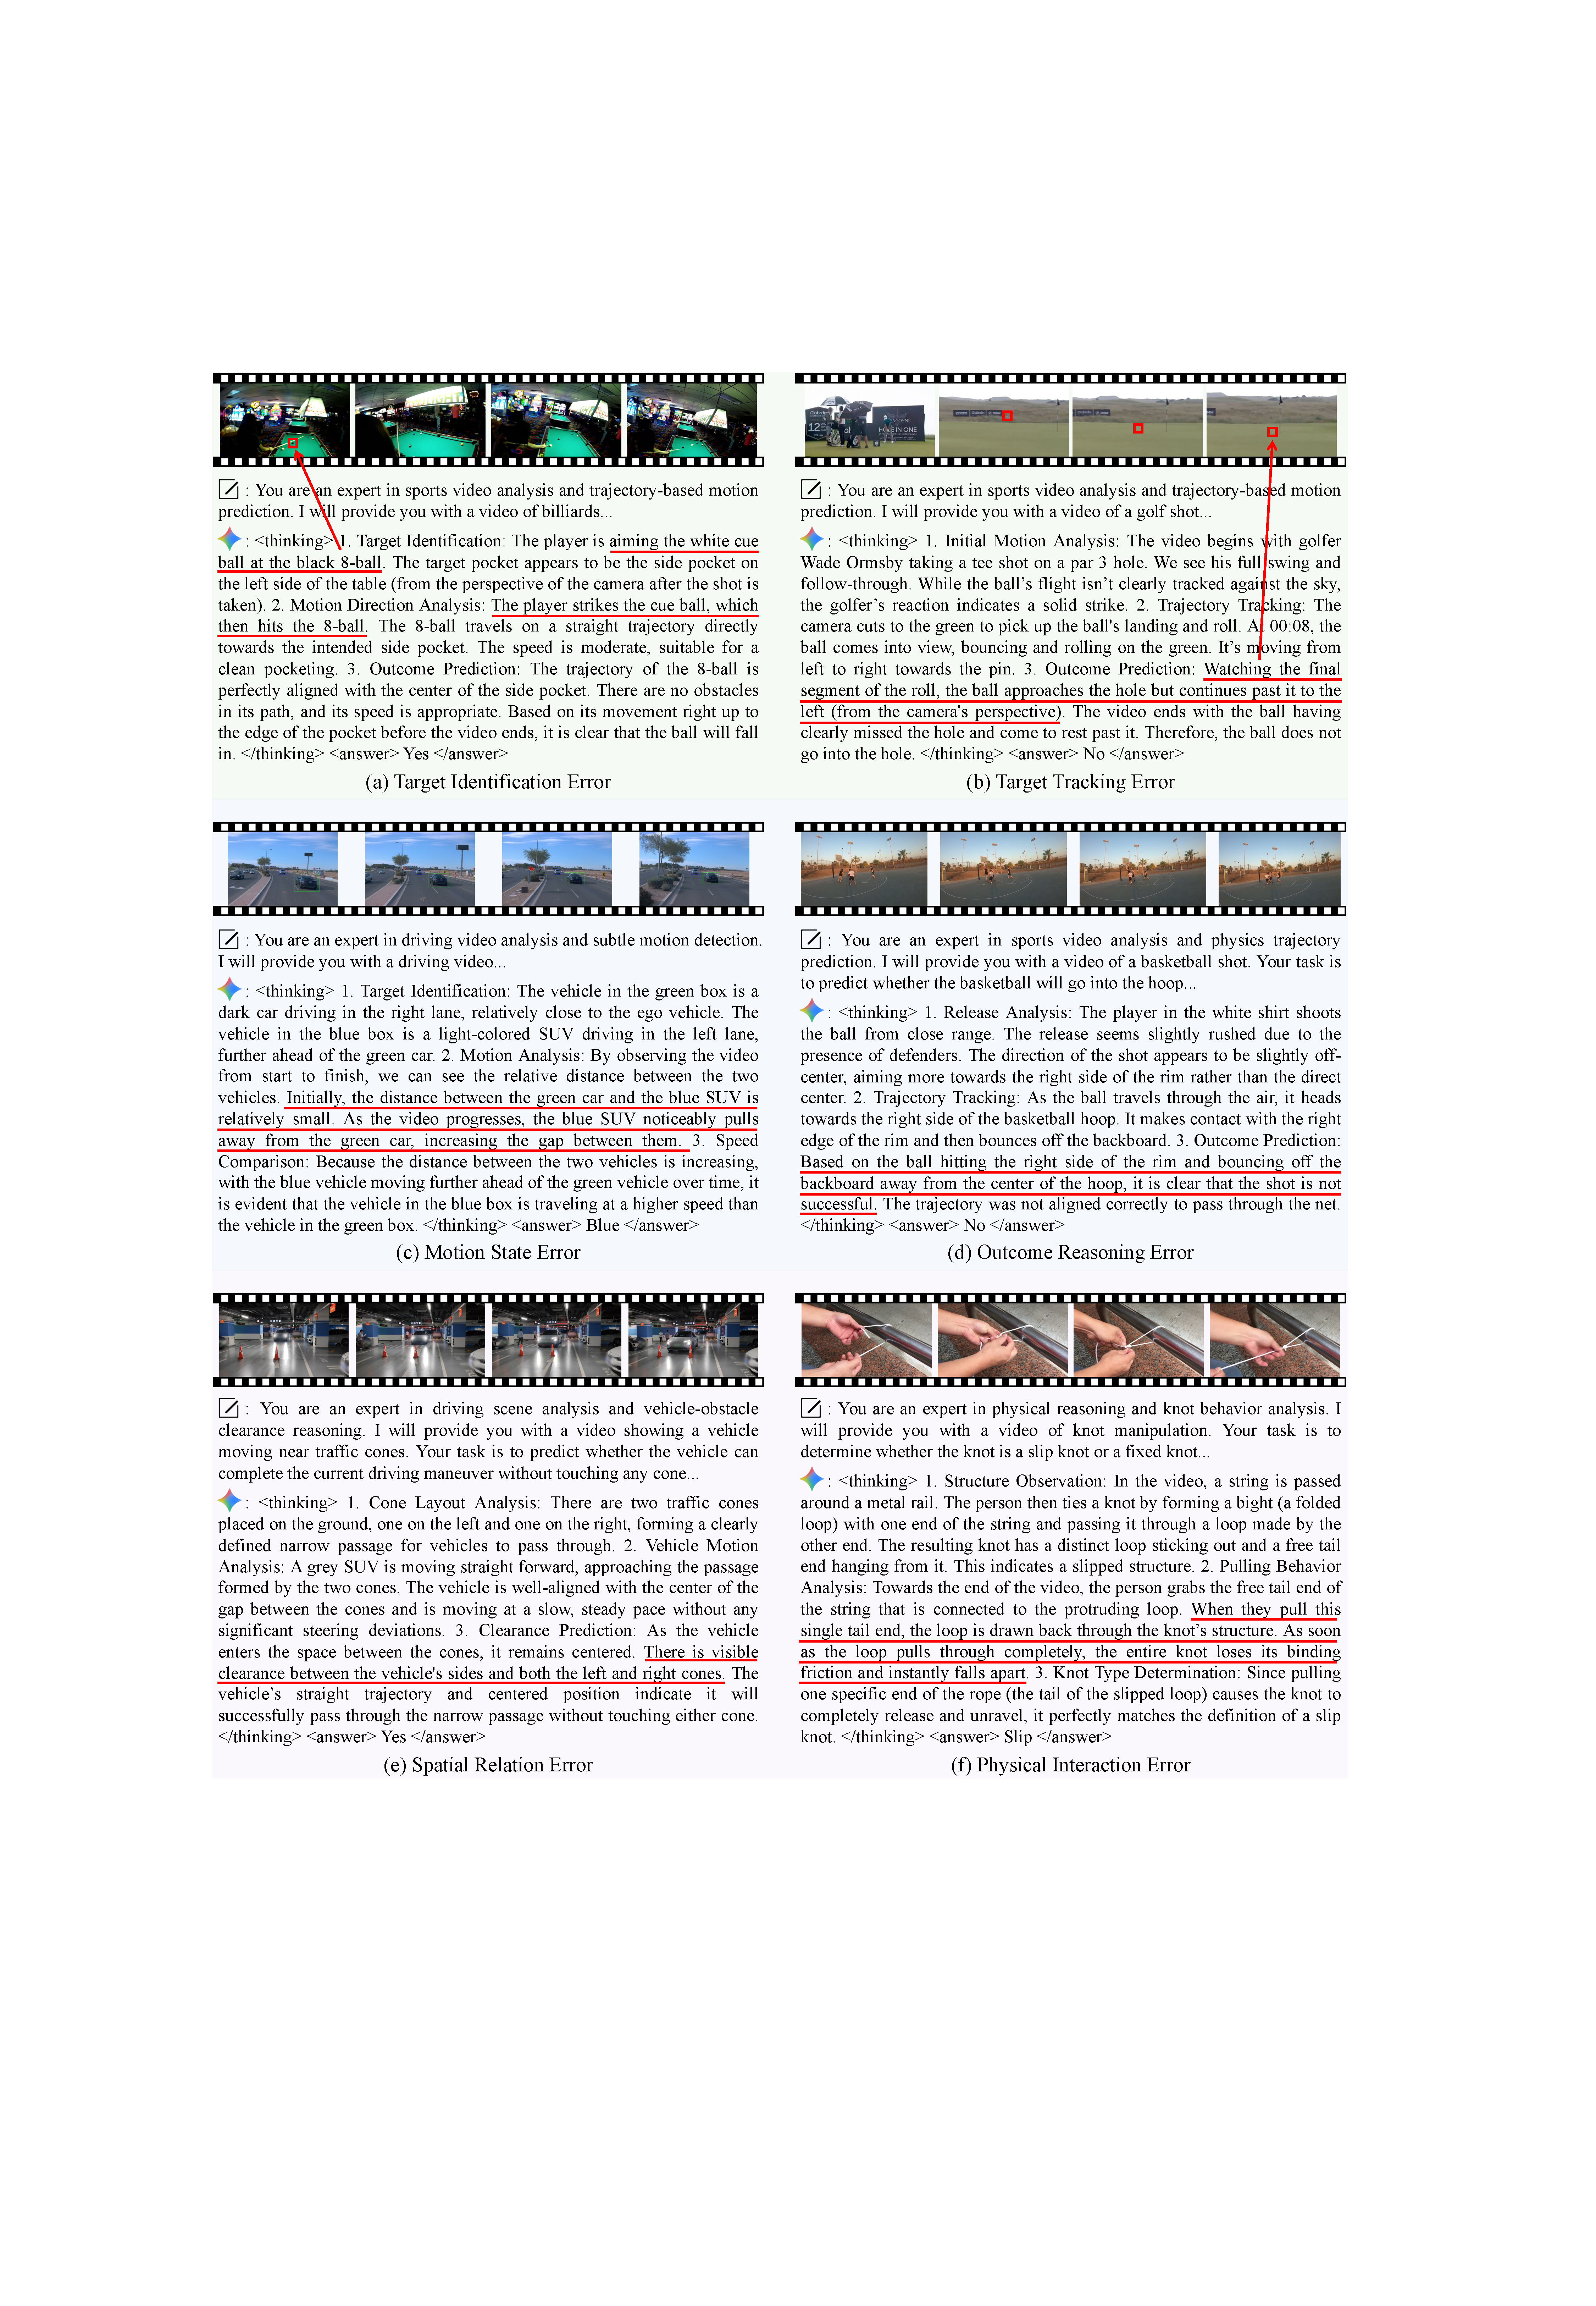
\includegraphics[width=0.95\linewidth]{fig/fig_18.pdf}
  \caption{\textbf{Representative examples for each primary error type.}}
  \label{fig:18}
\end{figure}

\begin{figure}[p]
  \centering
  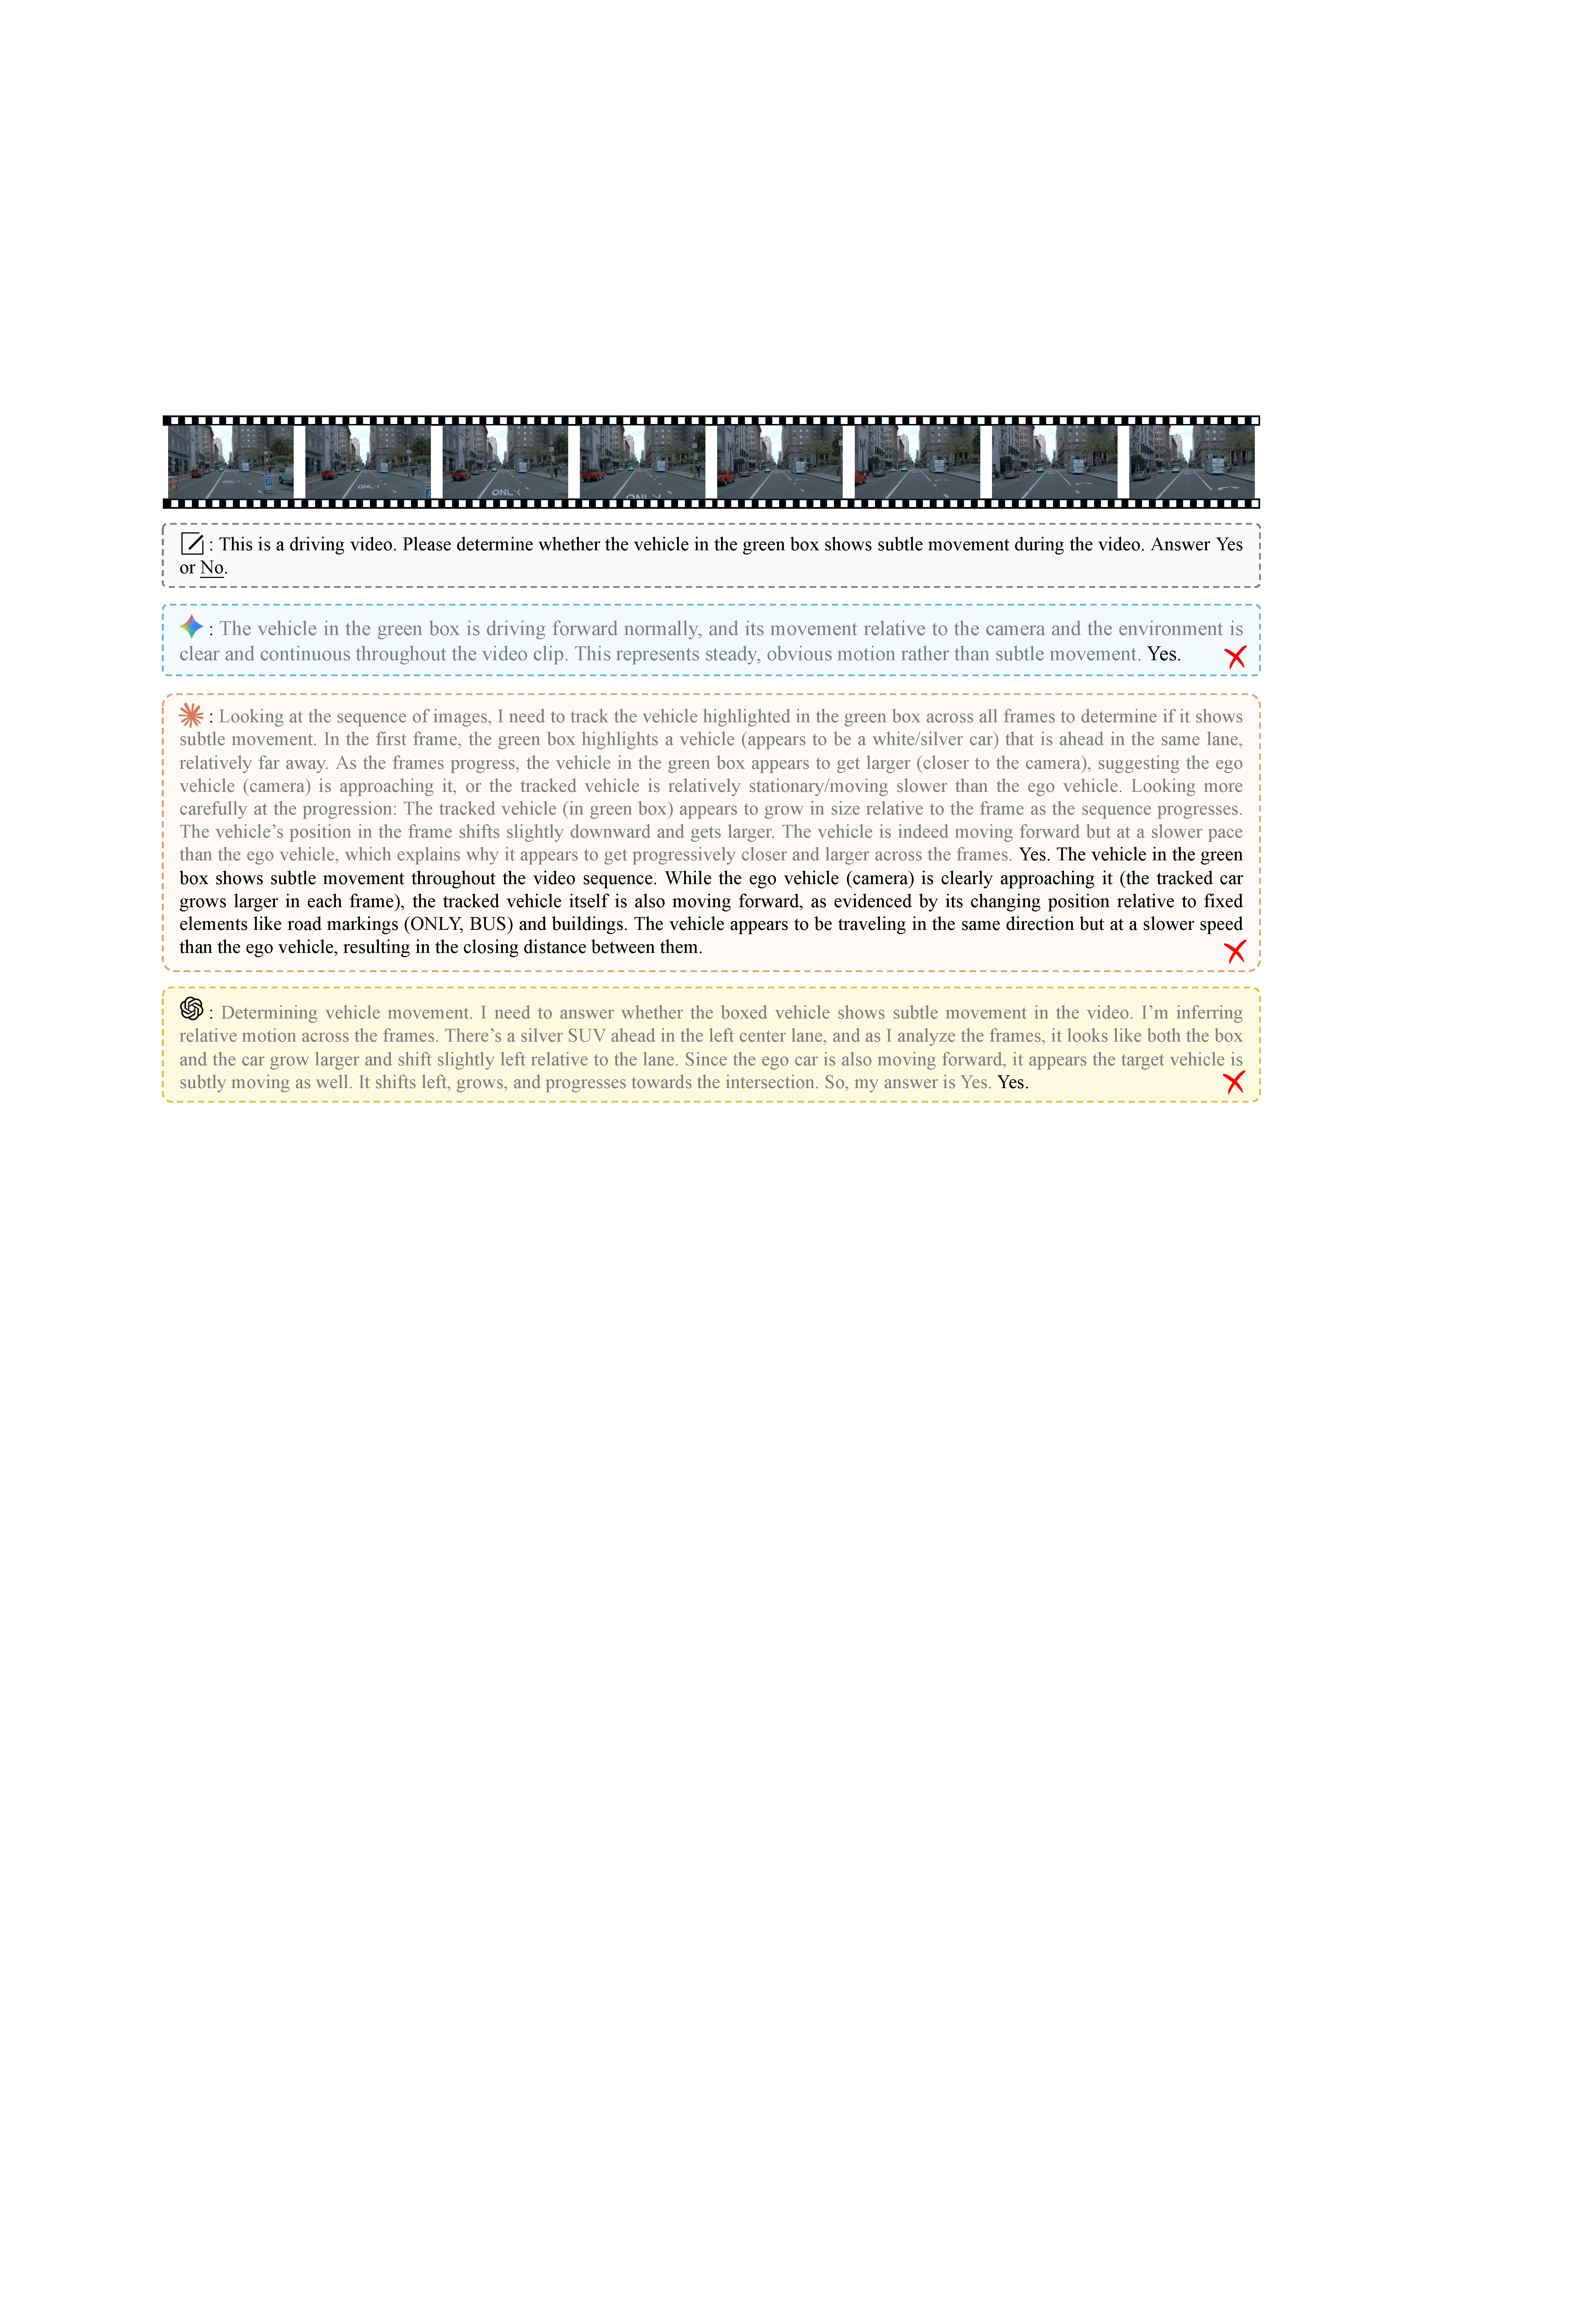
\includegraphics[width=0.95\linewidth]{fig/fig_19.pdf}
  \caption{\textbf{Qualitative visualization for Vehicle Movement.}
  We compare the outputs of GPT-5.4-thinking~\citep{GPT-5}, Gemini-3.1-Pro-Preview~\citep{Gemini}, and Claude-Opus-4.6-thinking~\citep{Claude}.
  Gray text denotes built-in thinking content.}
  \label{fig:19}
\end{figure}

\begin{figure}[p]
  \centering
  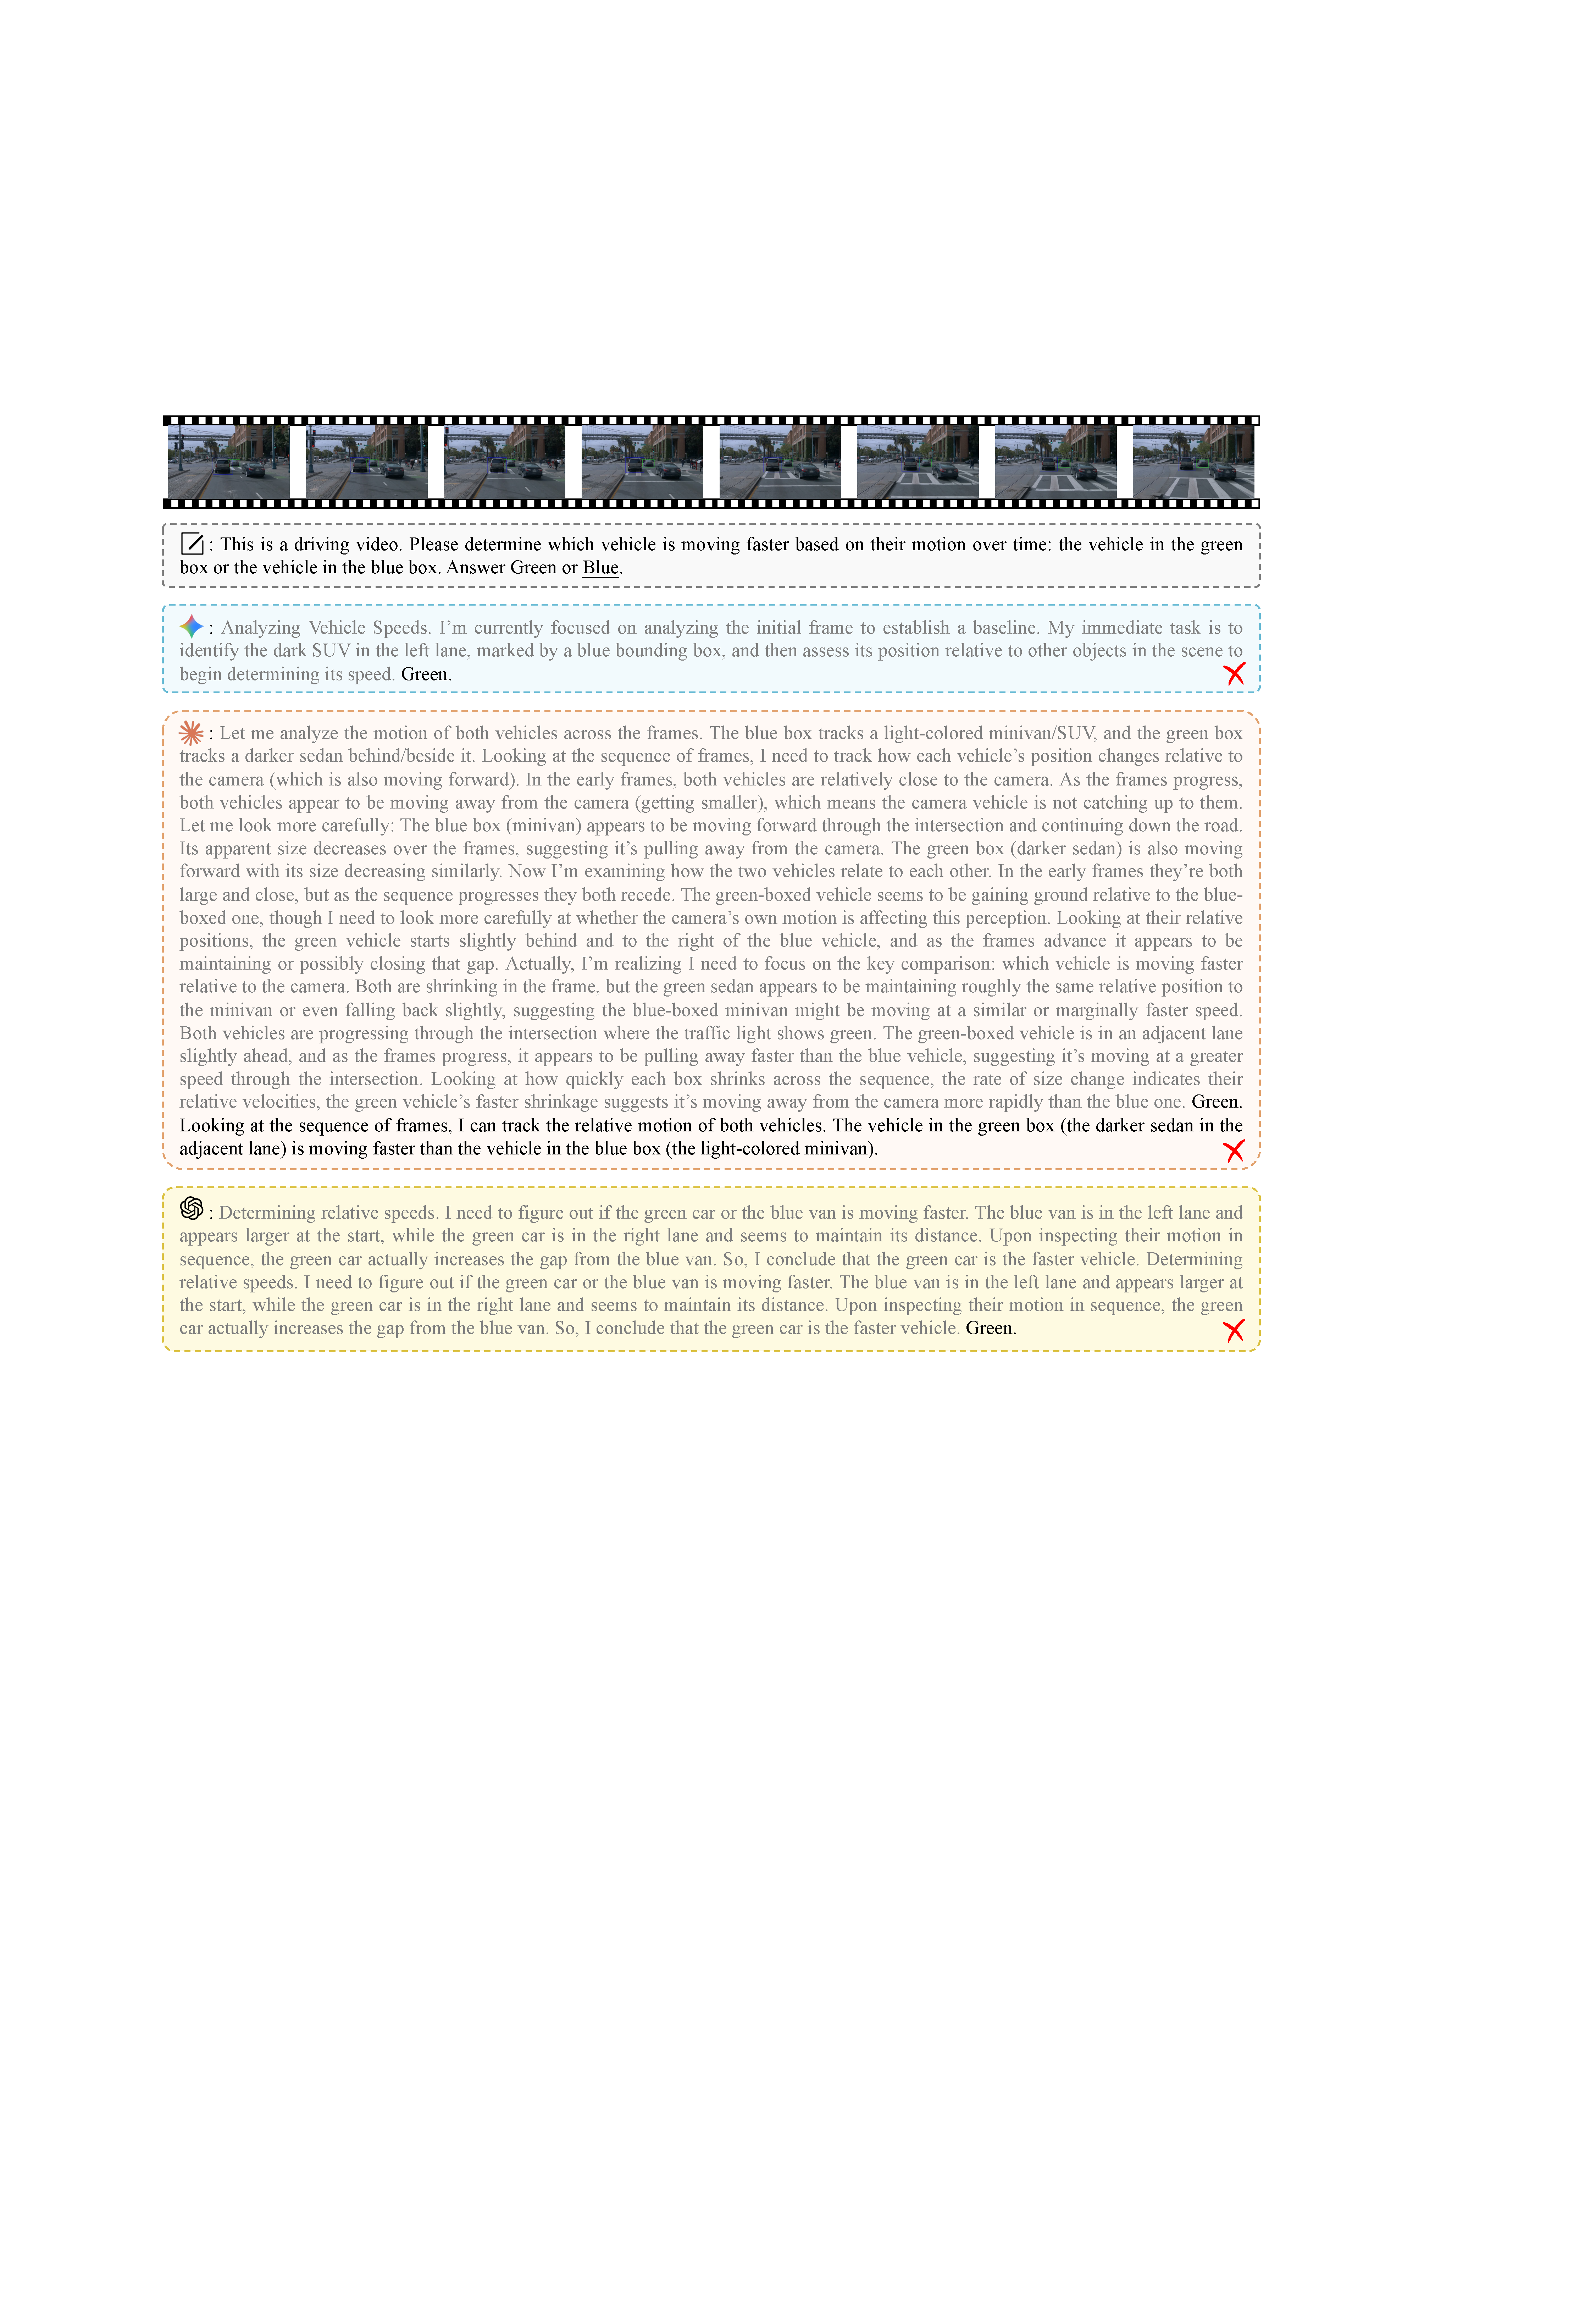
\includegraphics[width=0.95\linewidth]{fig/fig_20.pdf}
  \caption{\textbf{Qualitative visualization for Relative Velocity.}
  We compare the outputs of GPT-5.4-thinking~\citep{GPT-5}, Gemini-3.1-Pro-Preview~\citep{Gemini}, and Claude-Opus-4.6-thinking~\citep{Claude}.
  Gray text denotes built-in thinking content.}
  \label{fig:20}
\end{figure}

\begin{figure}[p]
  \centering
  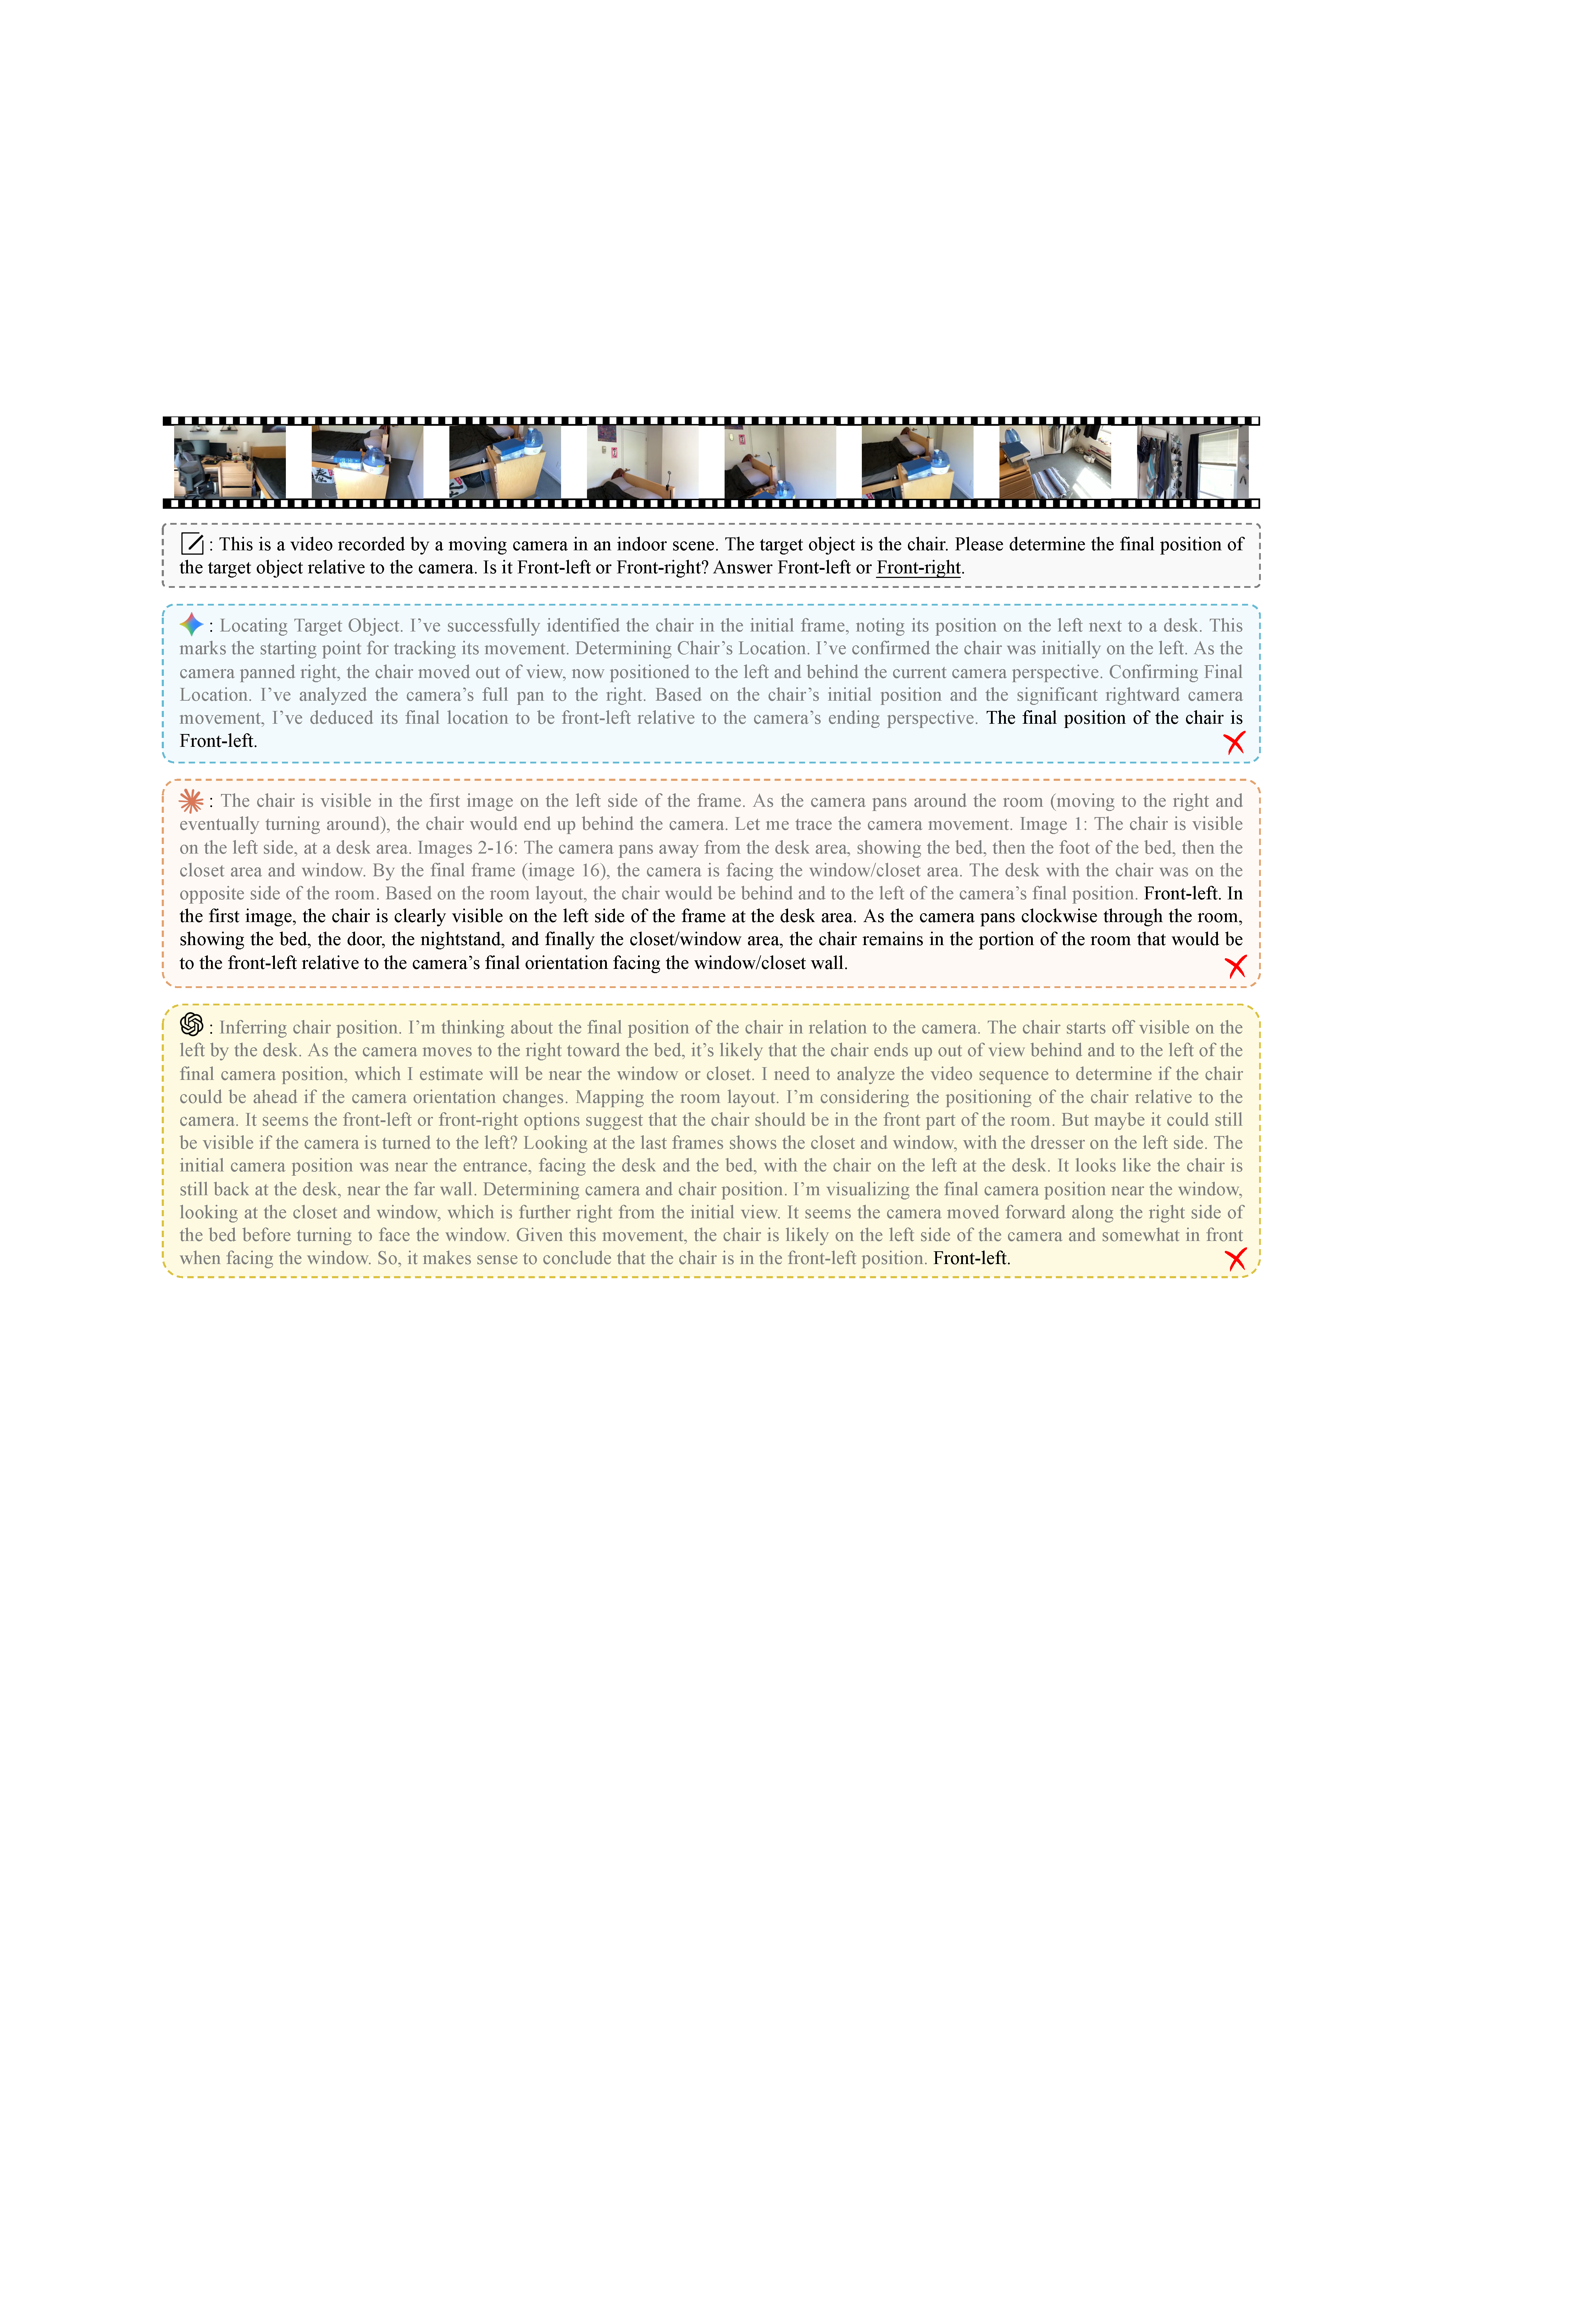
\includegraphics[width=0.95\linewidth]{fig/fig_21.pdf}
  \caption{\textbf{Qualitative visualization for Ego Motion.}
  We compare the outputs of GPT-5.4-thinking~\citep{GPT-5}, Gemini-3.1-Pro-Preview~\citep{Gemini}, and Claude-Opus-4.6-thinking~\citep{Claude}.
  Gray text denotes built-in thinking content.}
  \label{fig:21}
\end{figure}

\begin{figure}[p]
  \centering
  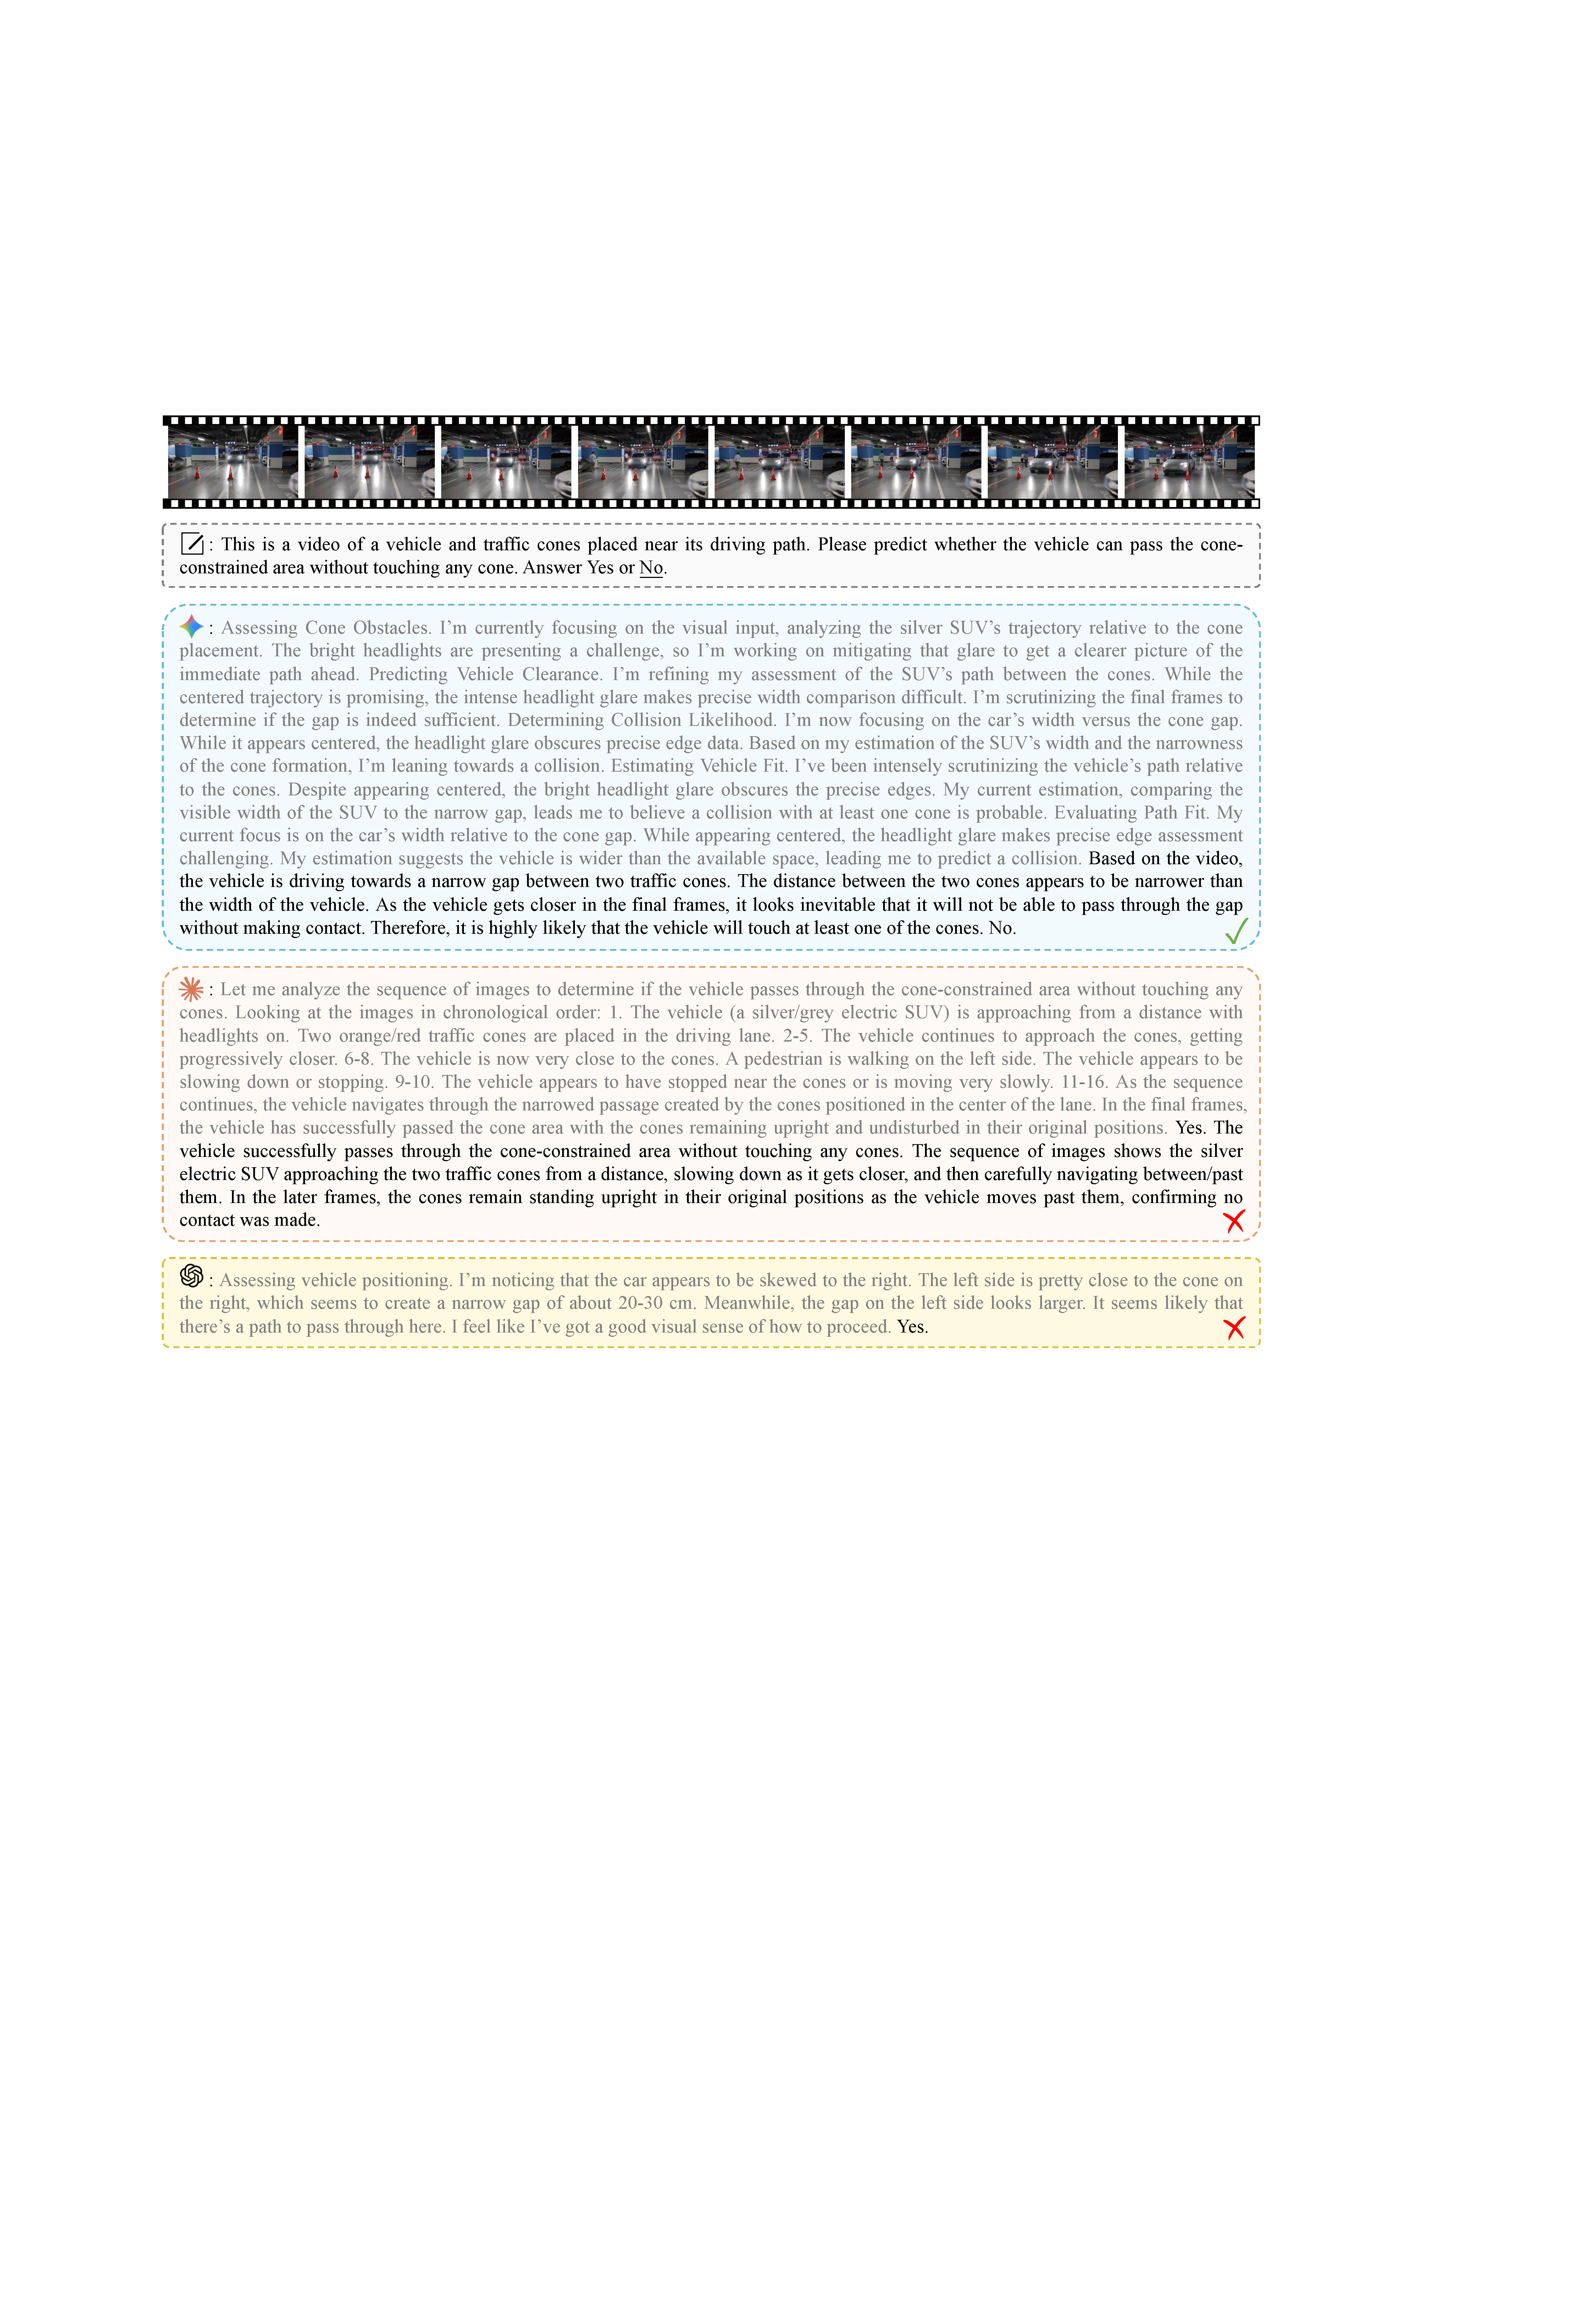
\includegraphics[width=0.95\linewidth]{fig/fig_22.pdf}
  \caption{\textbf{Qualitative visualization for Passage Feasibility.}
  We compare the outputs of GPT-5.4-thinking~\citep{GPT-5}, Gemini-3.1-Pro-Preview~\citep{Gemini}, and Claude-Opus-4.6-thinking~\citep{Claude}.
  Gray text denotes built-in thinking content.}
  \label{fig:22}
\end{figure}

\begin{figure}[p]
  \centering
  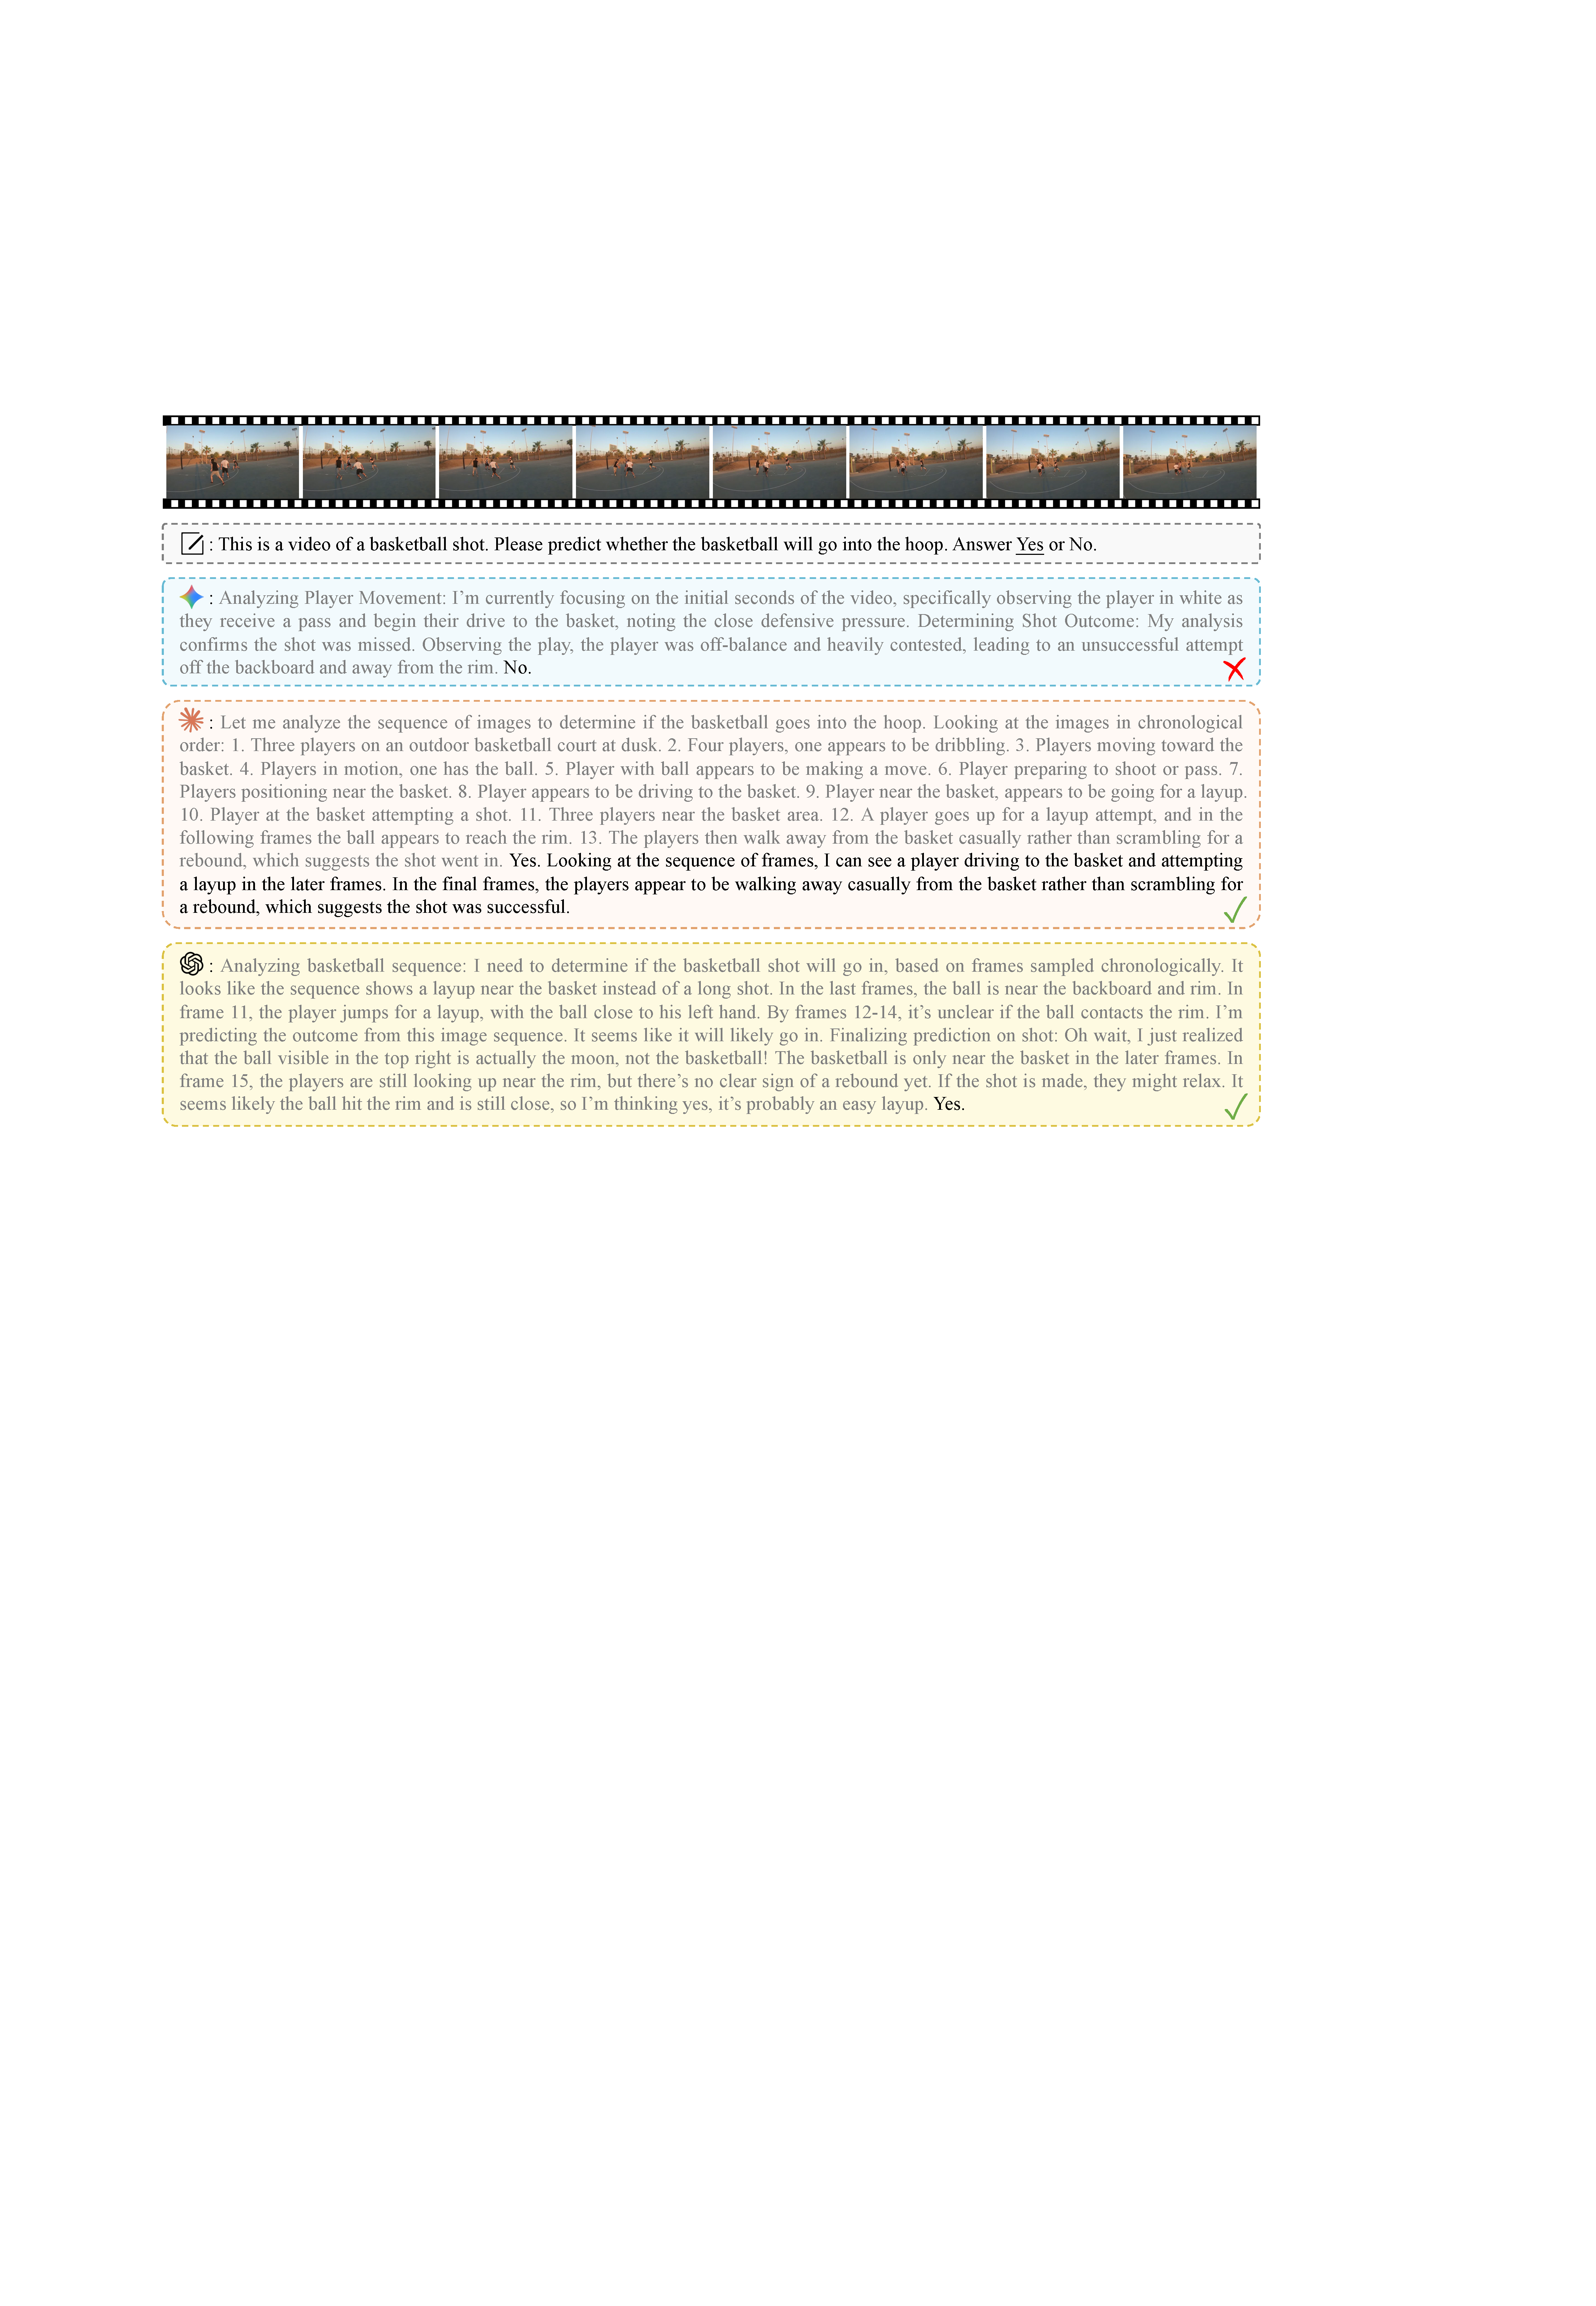
\includegraphics[width=0.95\linewidth]{fig/fig_23.pdf}
  \caption{\textbf{Qualitative visualization for Basketball Shot.}
  We compare the outputs of GPT-5.4-thinking~\citep{GPT-5}, Gemini-3.1-Pro-Preview~\citep{Gemini}, and Claude-Opus-4.6-thinking~\citep{Claude}.
  Gray text denotes built-in thinking content.}
  \label{fig:23}
\end{figure}

\begin{figure}[p]
  \centering
  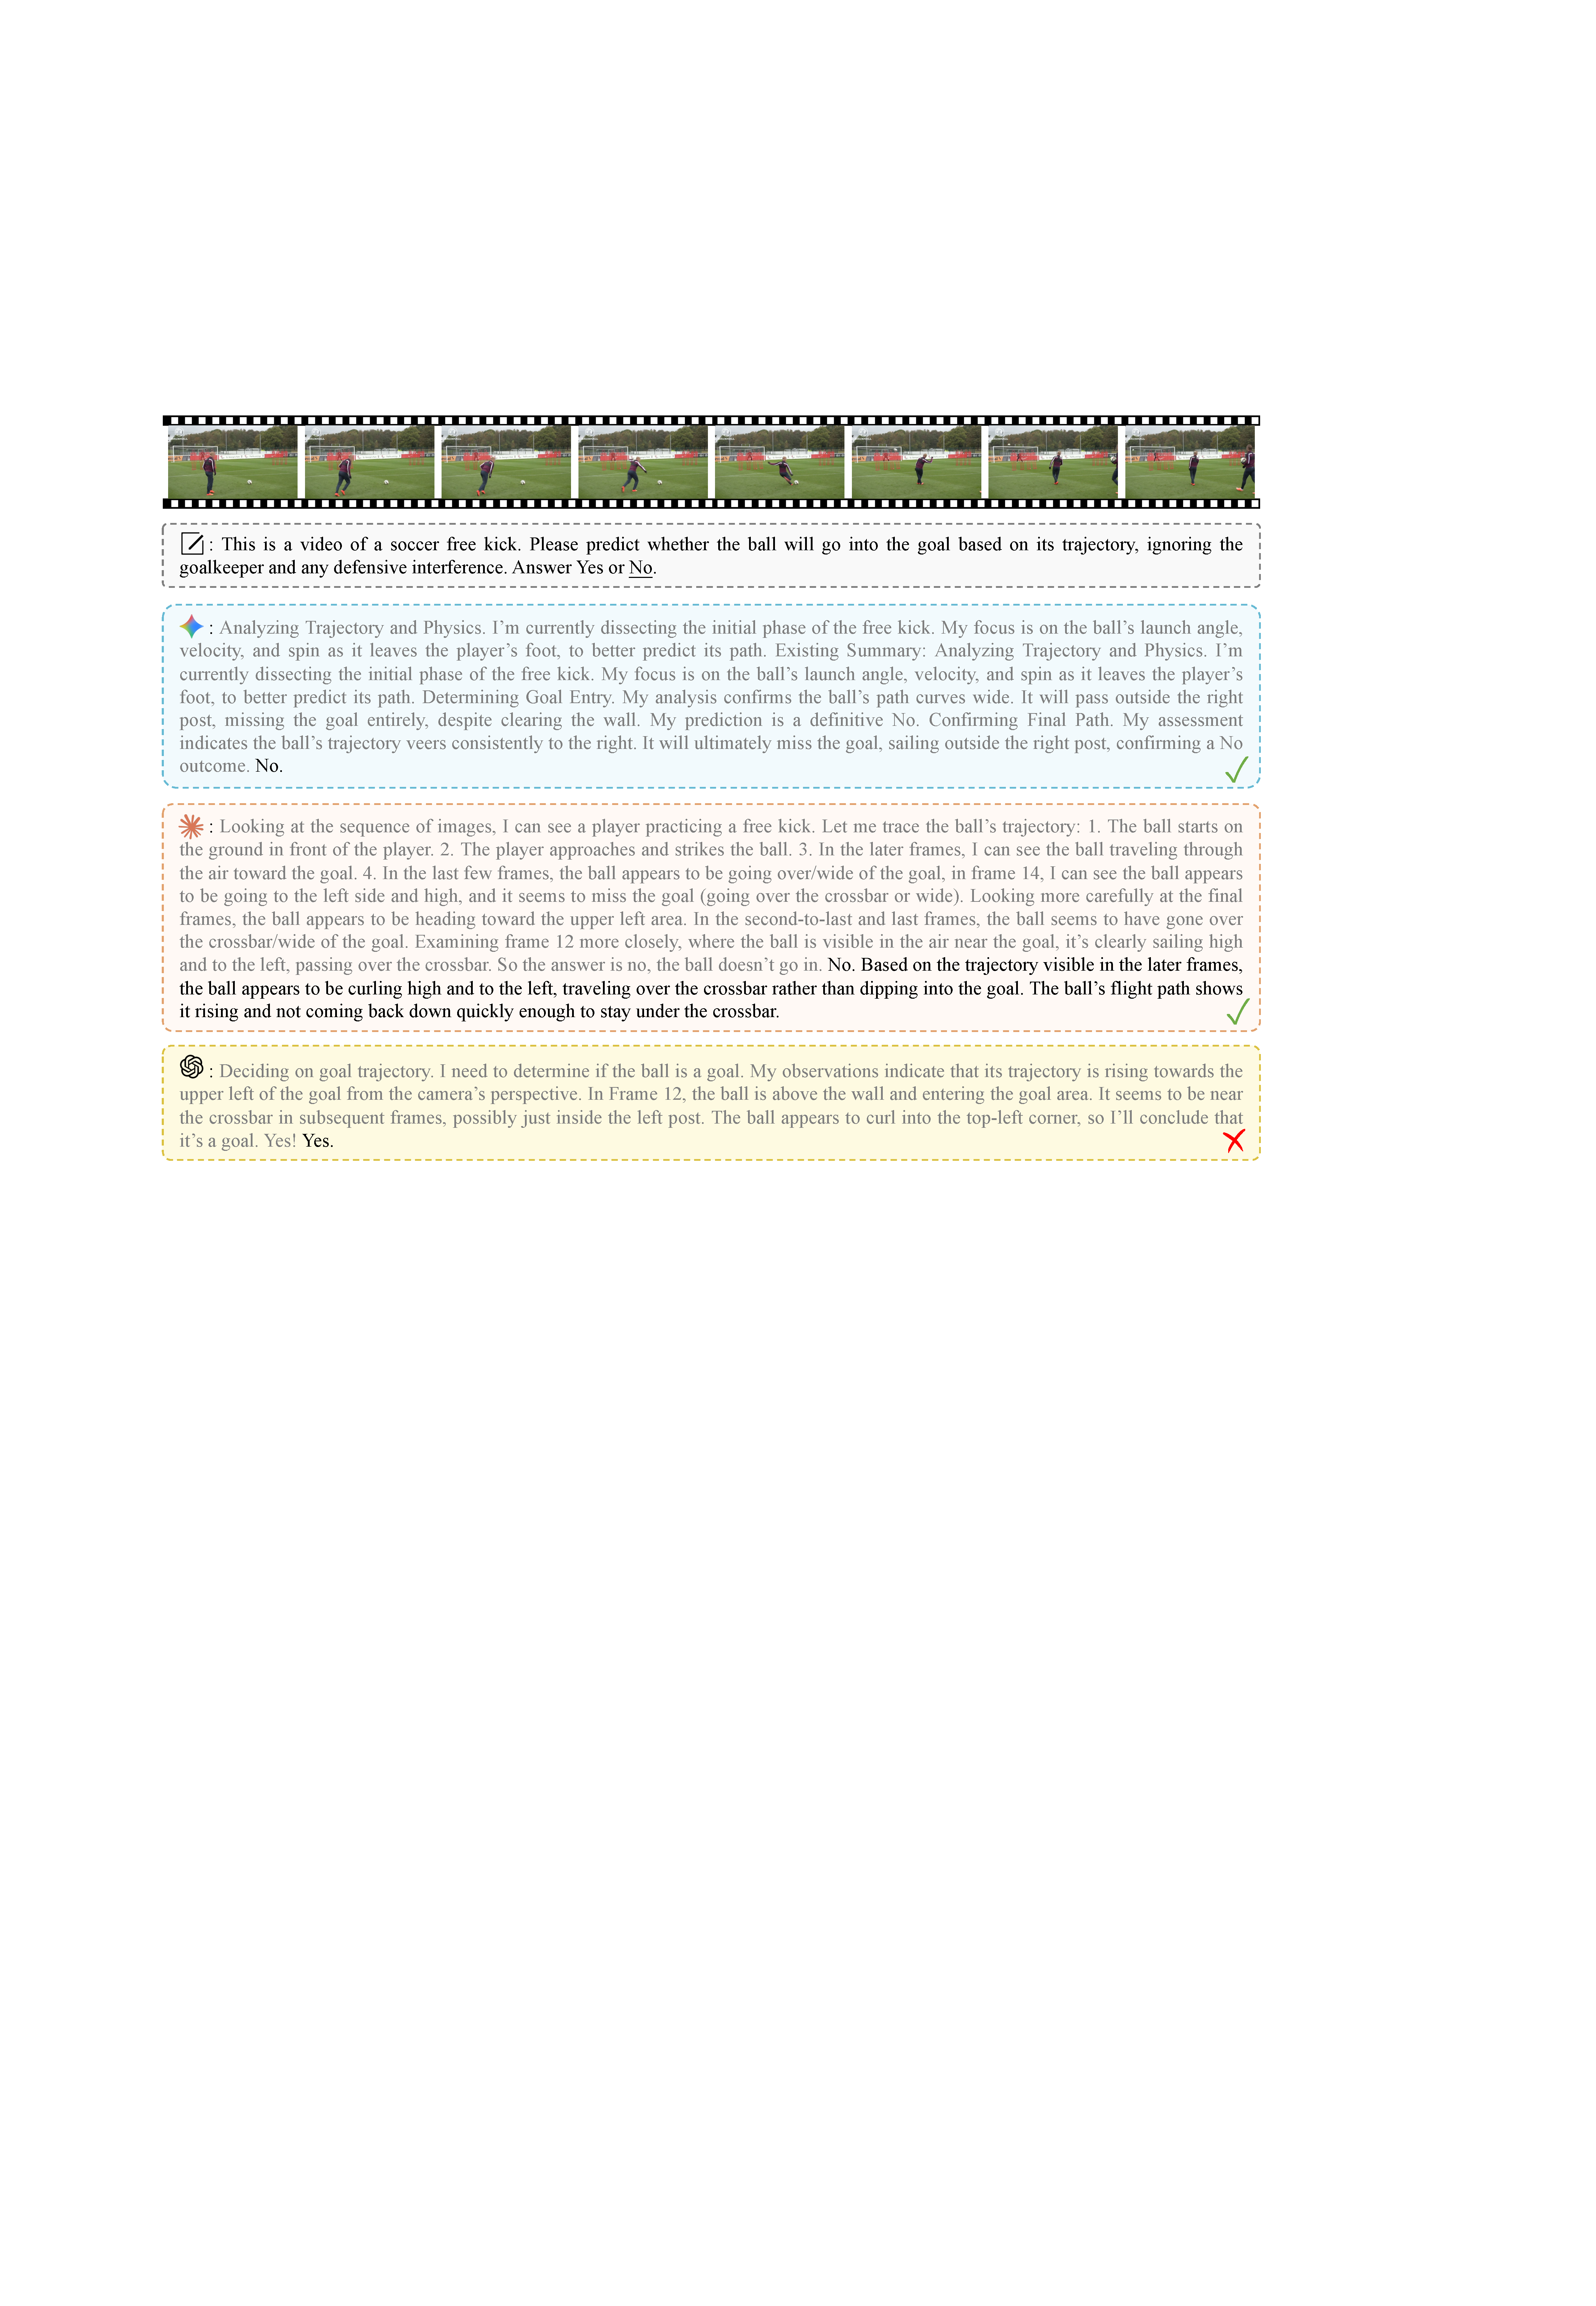
\includegraphics[width=0.95\linewidth]{fig/fig_24.pdf}
  \caption{\textbf{Qualitative visualization for Soccer Shot.}
  We compare the outputs of GPT-5.4-thinking~\citep{GPT-5}, Gemini-3.1-Pro-Preview~\citep{Gemini}, and Claude-Opus-4.6-thinking~\citep{Claude}.
  Gray text denotes built-in thinking content.}
  \label{fig:24}
\end{figure}

\begin{figure}[p]
  \centering
  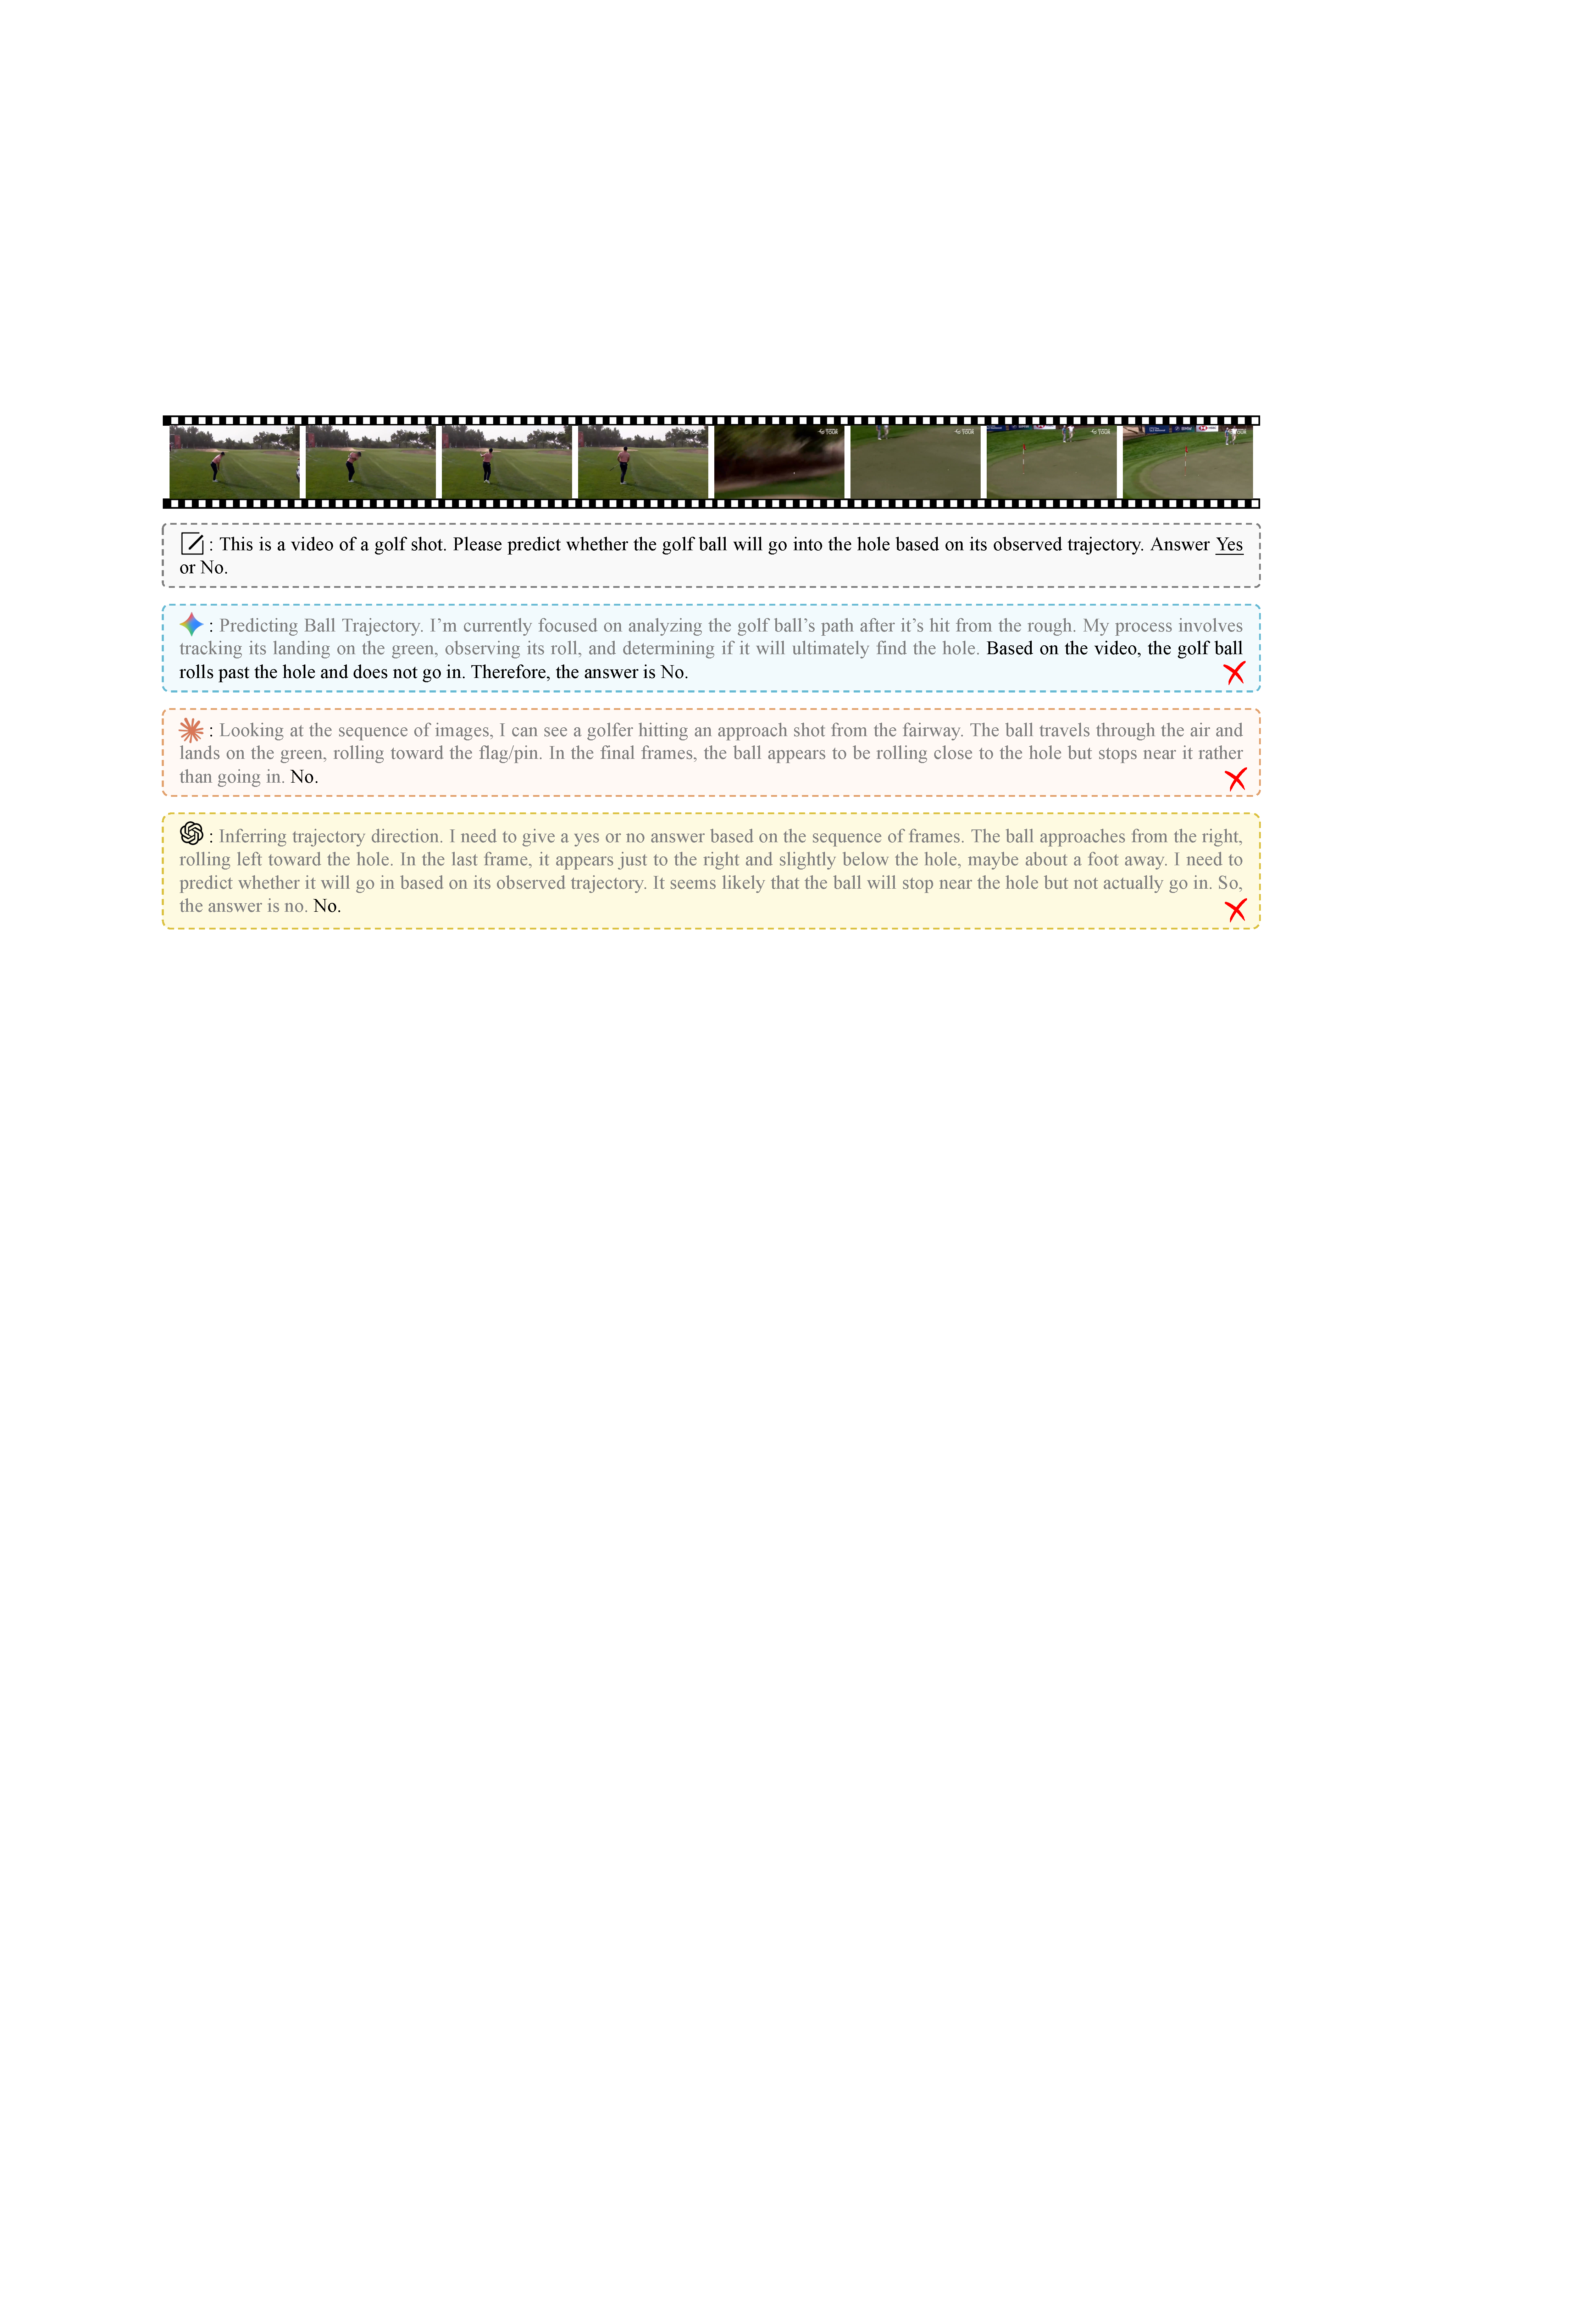
\includegraphics[width=0.95\linewidth]{fig/fig_25.pdf}
  \caption{\textbf{Qualitative visualization for Golf Shot.}
  We compare the outputs of GPT-5.4-thinking~\citep{GPT-5}, Gemini-3.1-Pro-Preview~\citep{Gemini}, and Claude-Opus-4.6-thinking~\citep{Claude}.
  Gray text denotes built-in thinking content.}
  \label{fig:25}
\end{figure}

\begin{figure}[p]
  \centering
  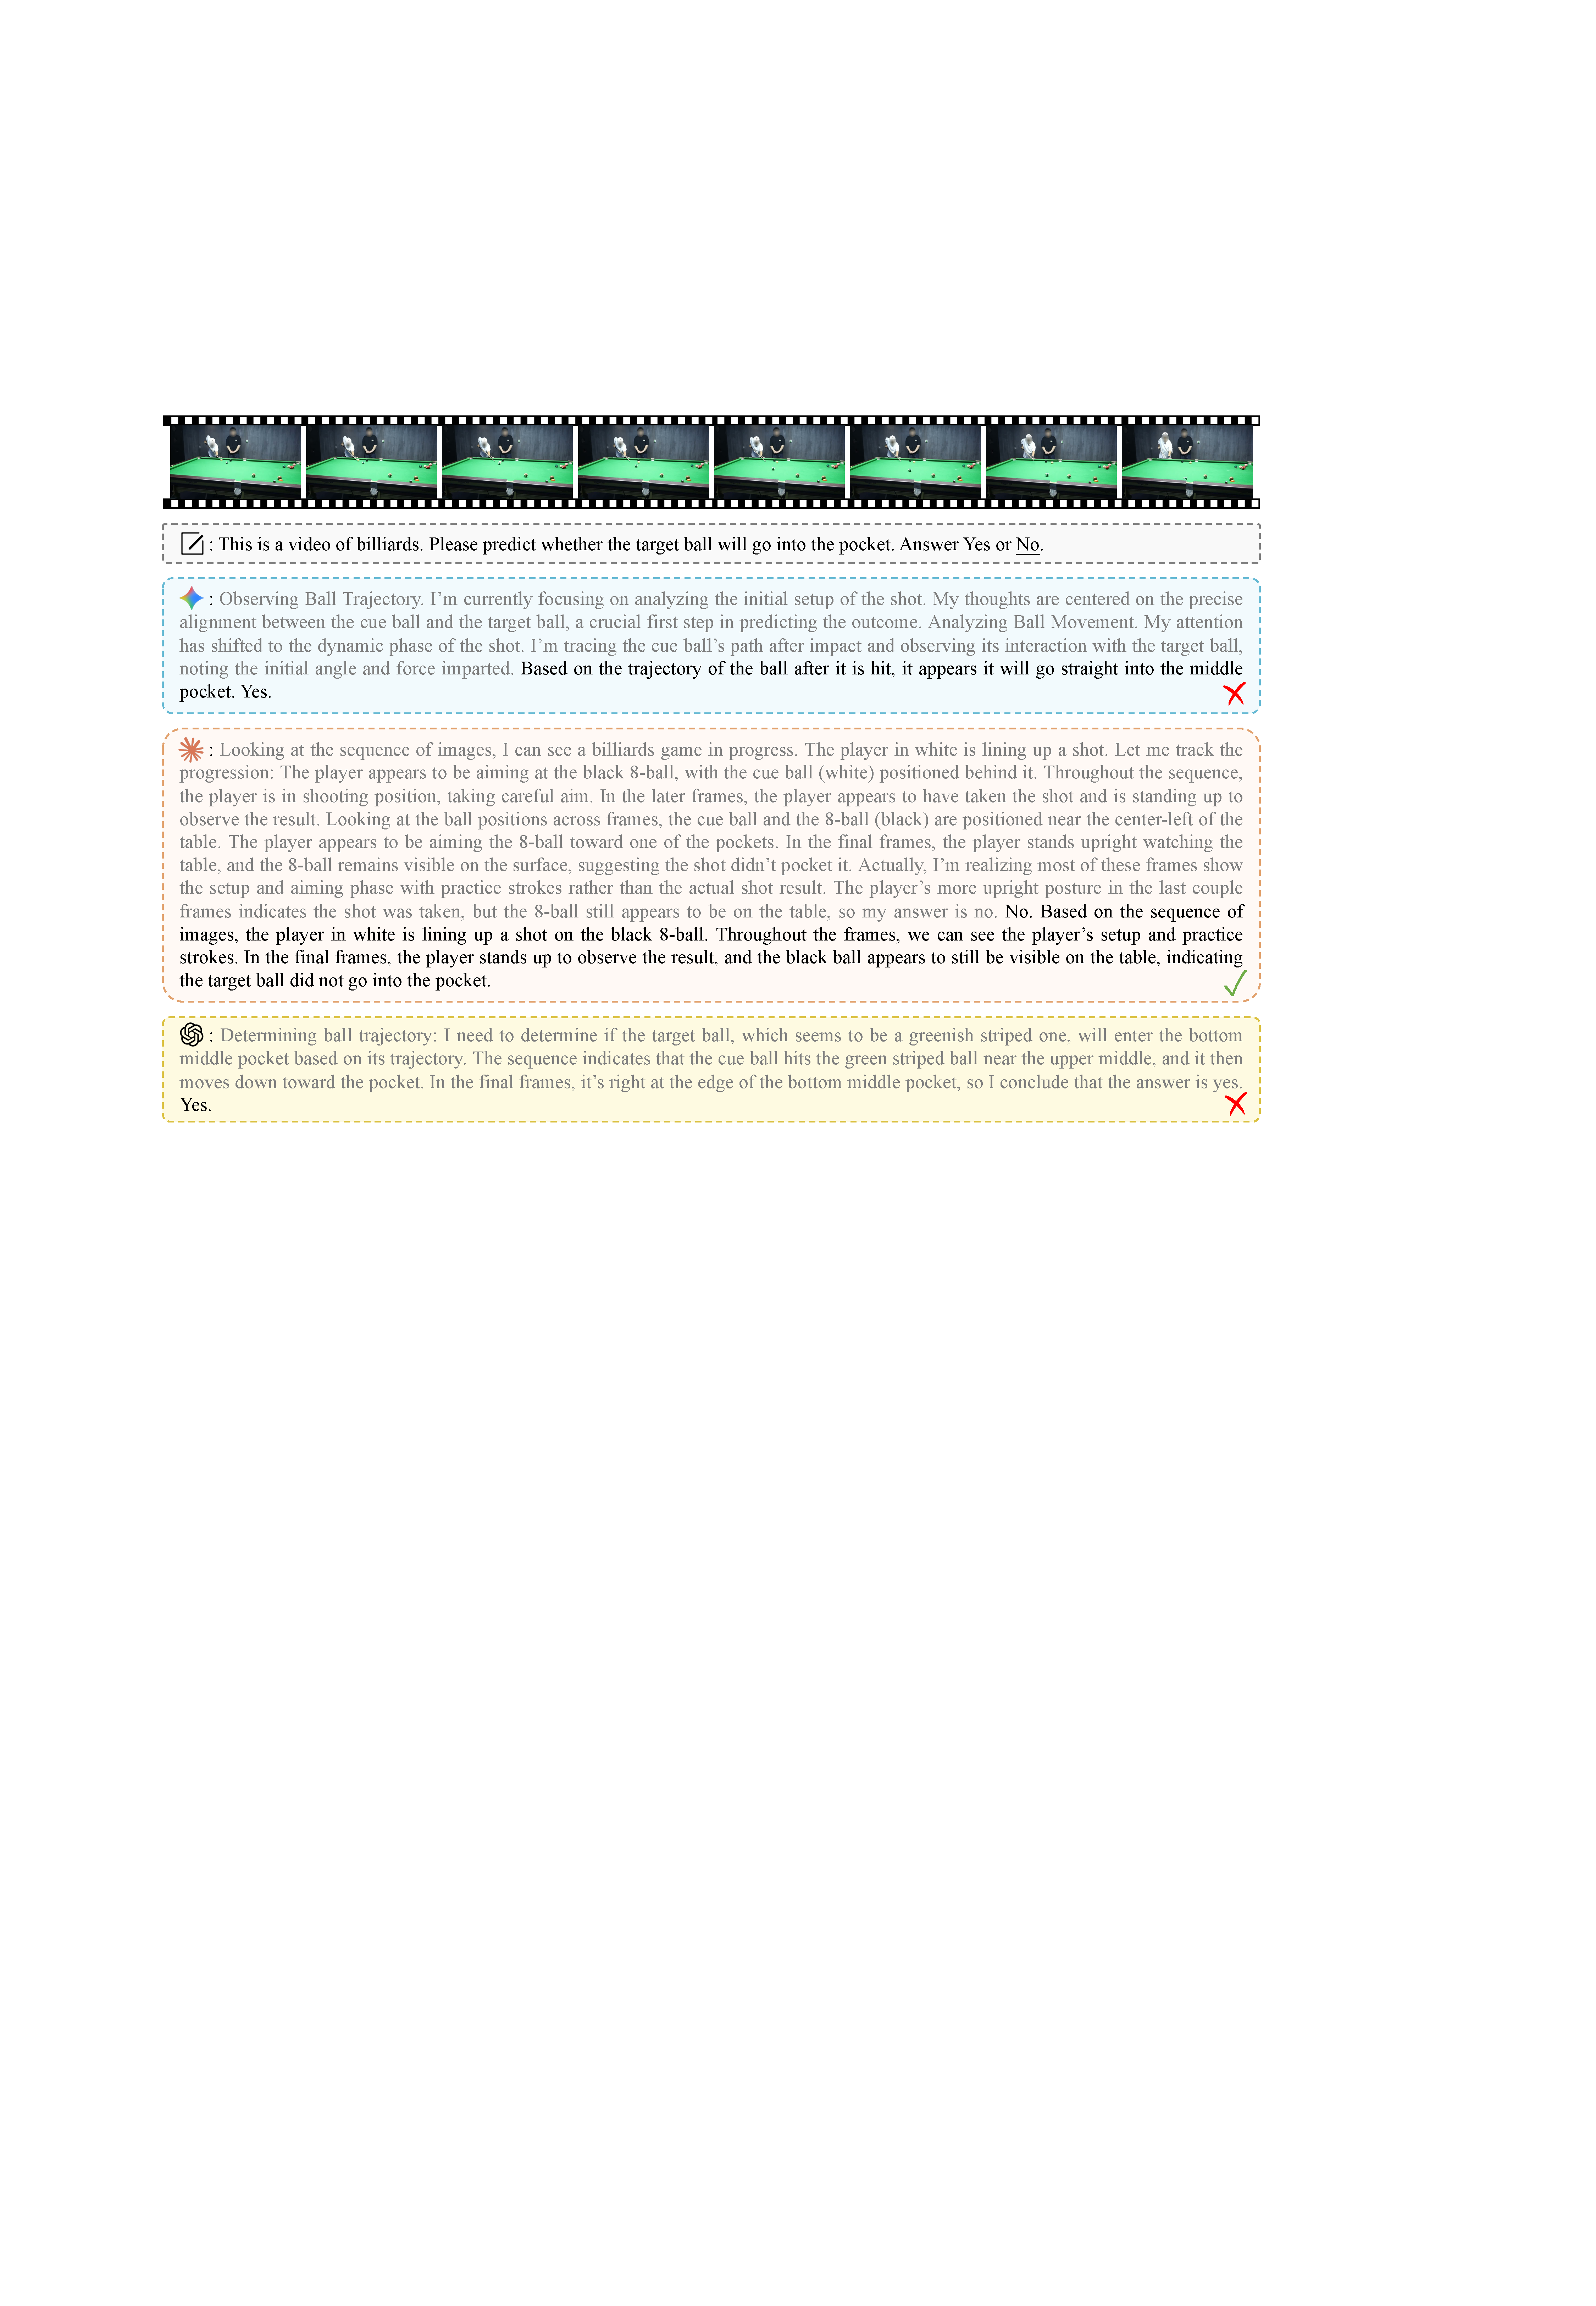
\includegraphics[width=0.95\linewidth]{fig/fig_26.pdf}
  \caption{\textbf{Qualitative visualization for Billiards Shot.}
  We compare the outputs of GPT-5.4-thinking~\citep{GPT-5}, Gemini-3.1-Pro-Preview~\citep{Gemini}, and Claude-Opus-4.6-thinking~\citep{Claude}.
  Gray text denotes built-in thinking content.}
  \label{fig:26}
\end{figure}

\begin{figure}[p]
  \centering
  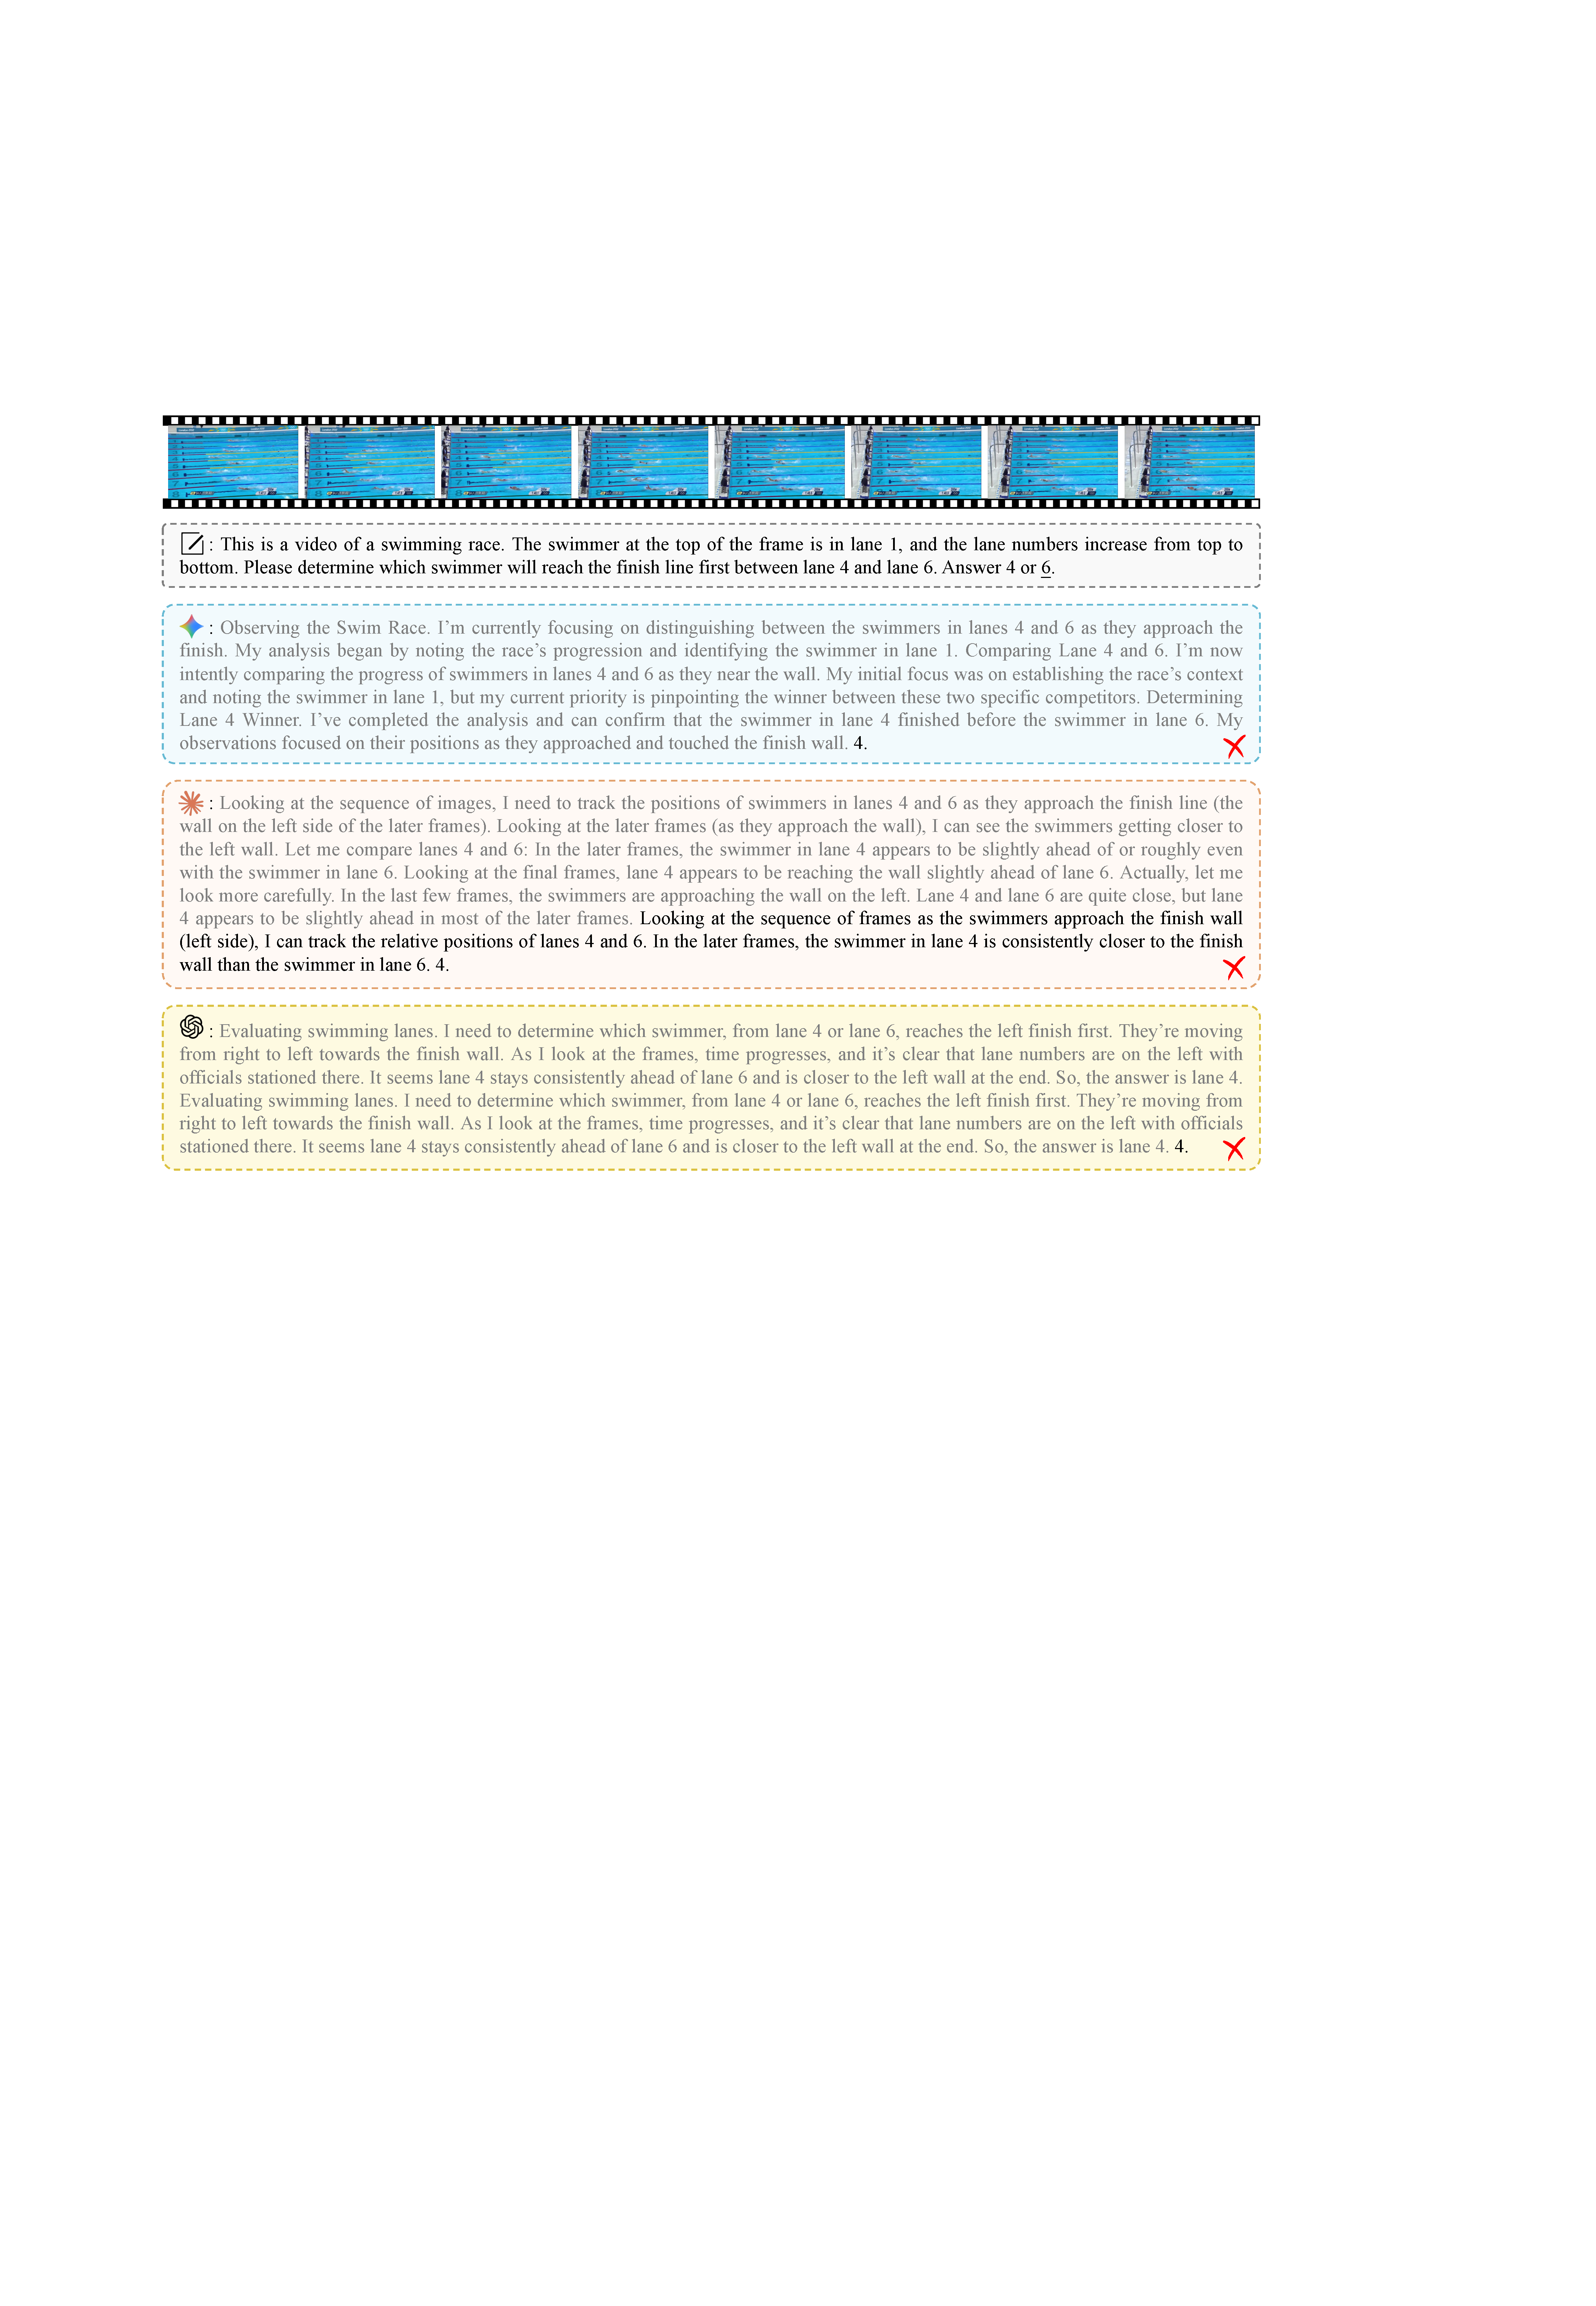
\includegraphics[width=0.95\linewidth]{fig/fig_27.pdf}
  \caption{\textbf{Qualitative visualization for Swimming Race.}
  We compare the outputs of GPT-5.4-thinking~\citep{GPT-5}, Gemini-3.1-Pro-Preview~\citep{Gemini}, and Claude-Opus-4.6-thinking~\citep{Claude}.
  Gray text denotes built-in thinking content.}
  \label{fig:27}
\end{figure}

\begin{figure}[p]
  \centering
  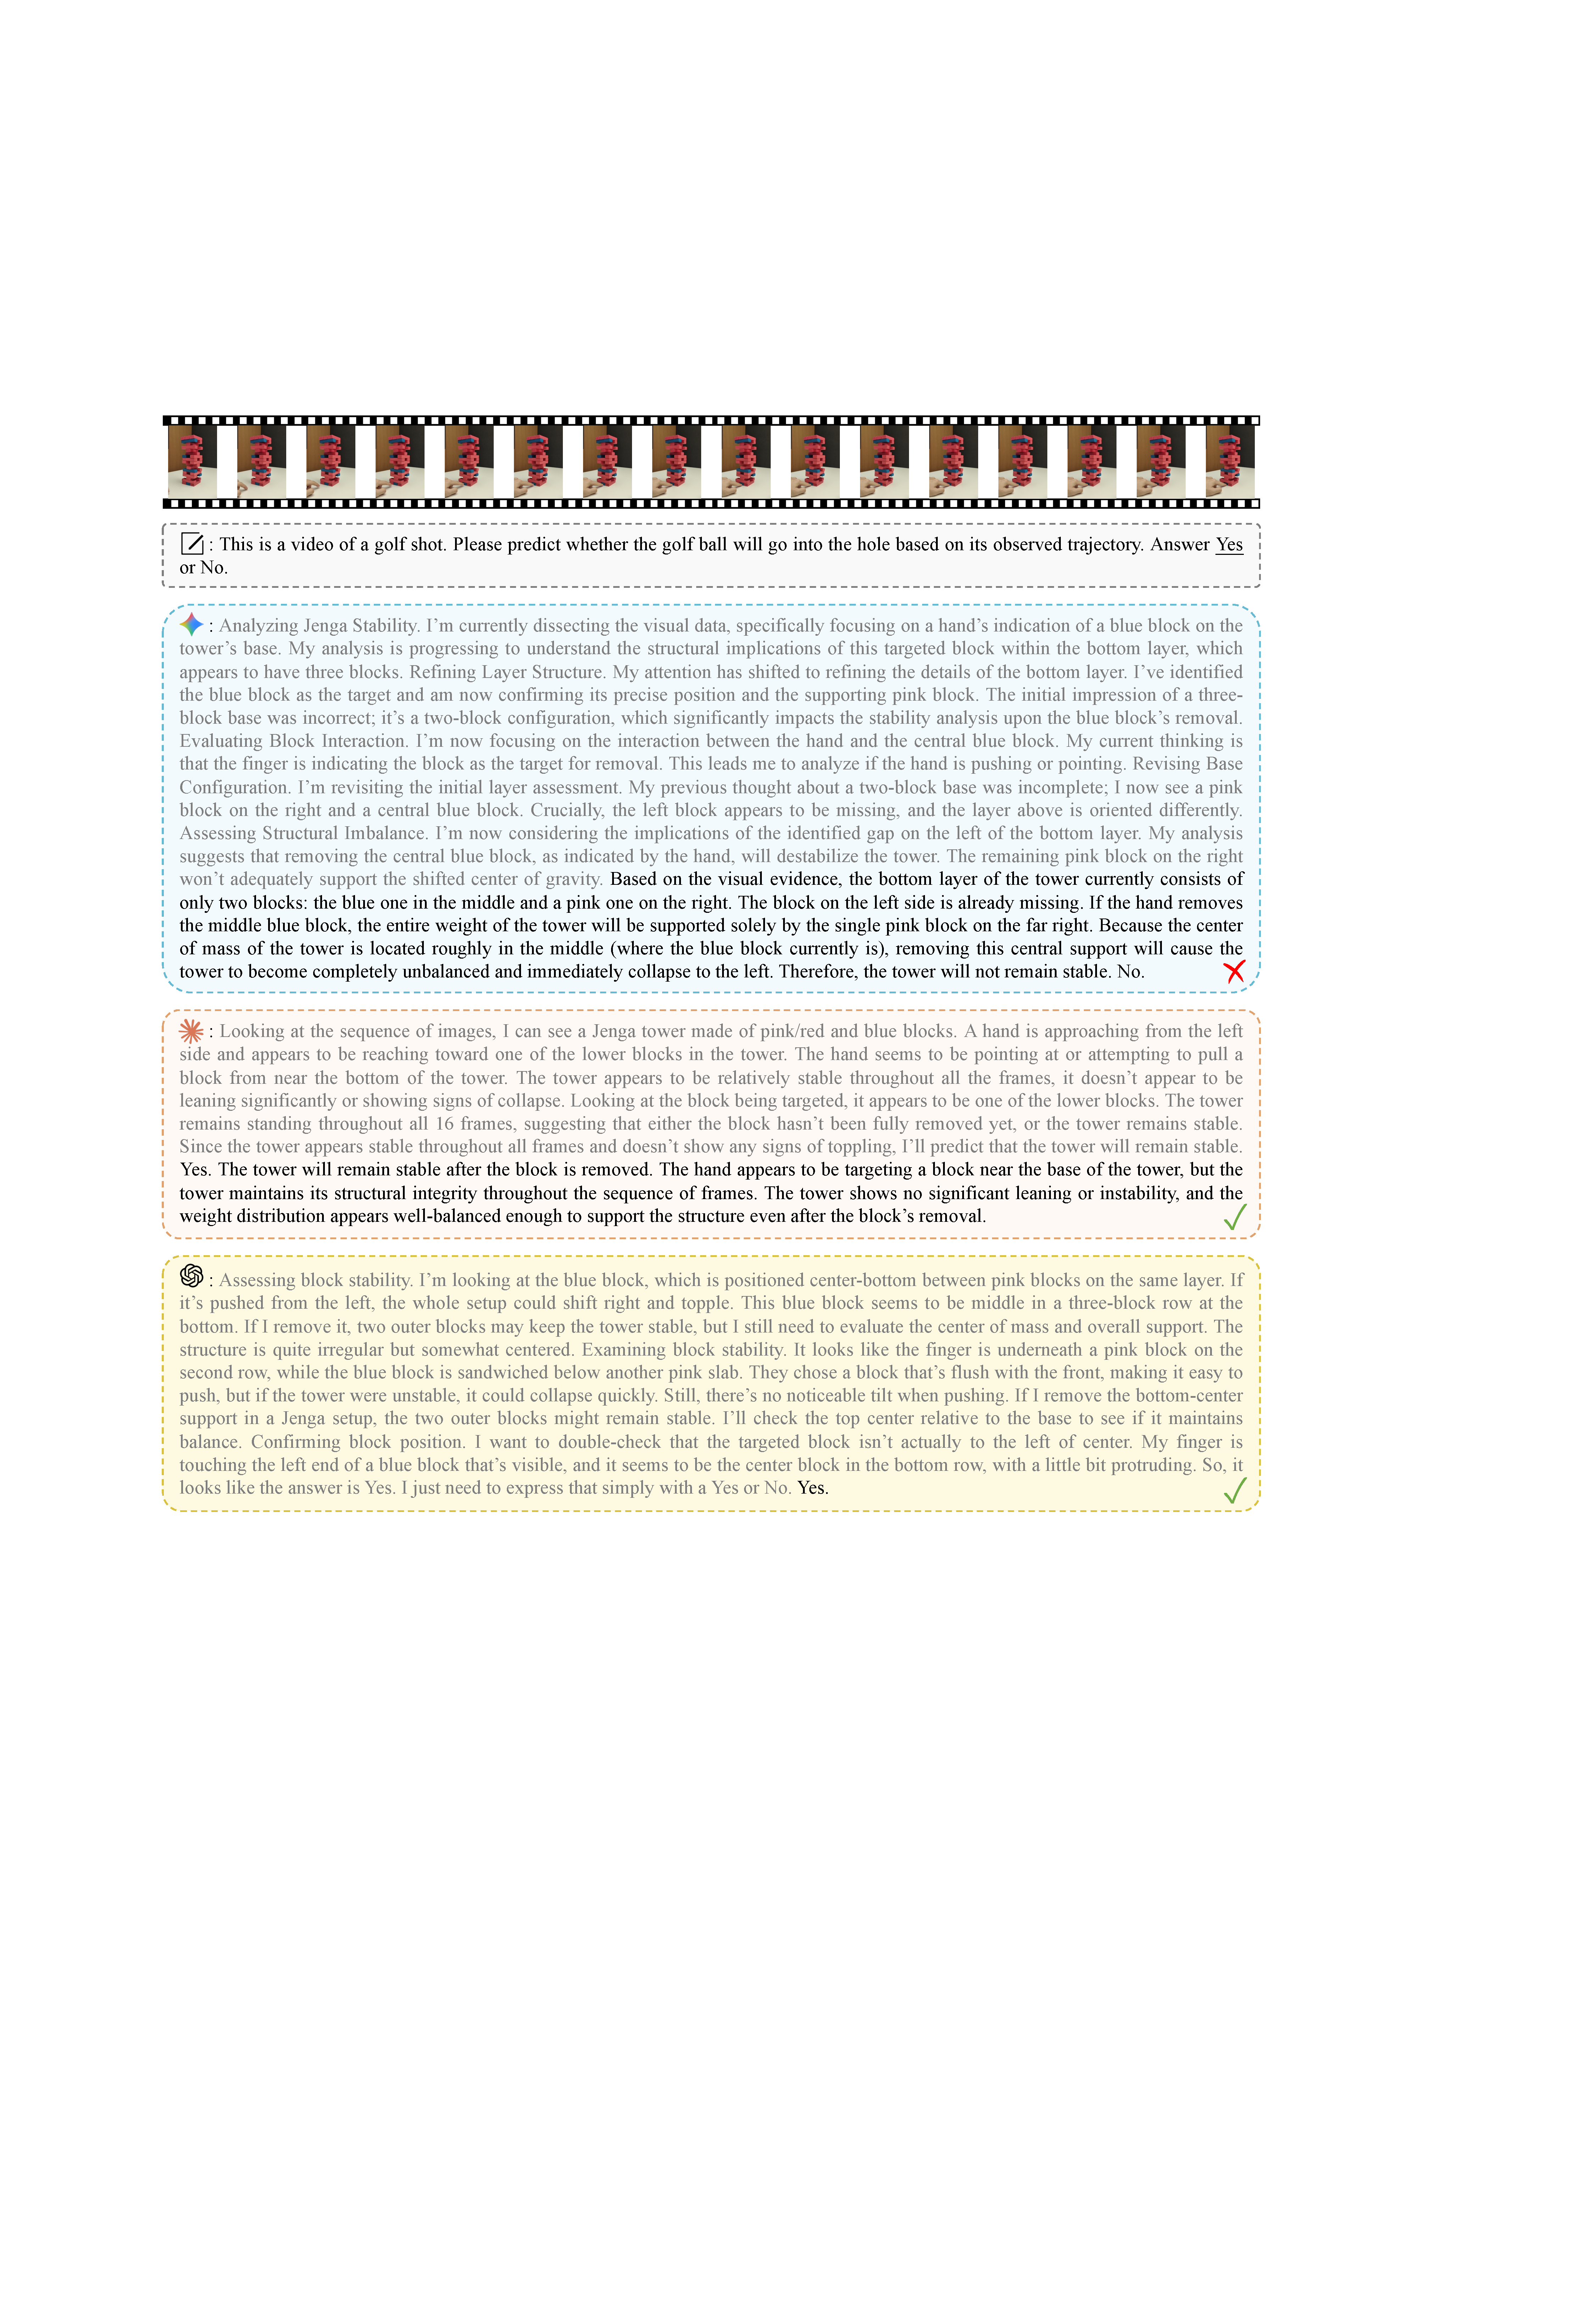
\includegraphics[width=0.95\linewidth]{fig/fig_28.pdf}
  \caption{\textbf{Qualitative visualization for Jenga Stability.}
  We compare the outputs of GPT-5.4-thinking~\citep{GPT-5}, Gemini-3.1-Pro-Preview~\citep{Gemini}, and Claude-Opus-4.6-thinking~\citep{Claude}.
  Gray text denotes built-in thinking content.}
  \label{fig:28}
\end{figure}

\begin{figure}[p]
  \centering
  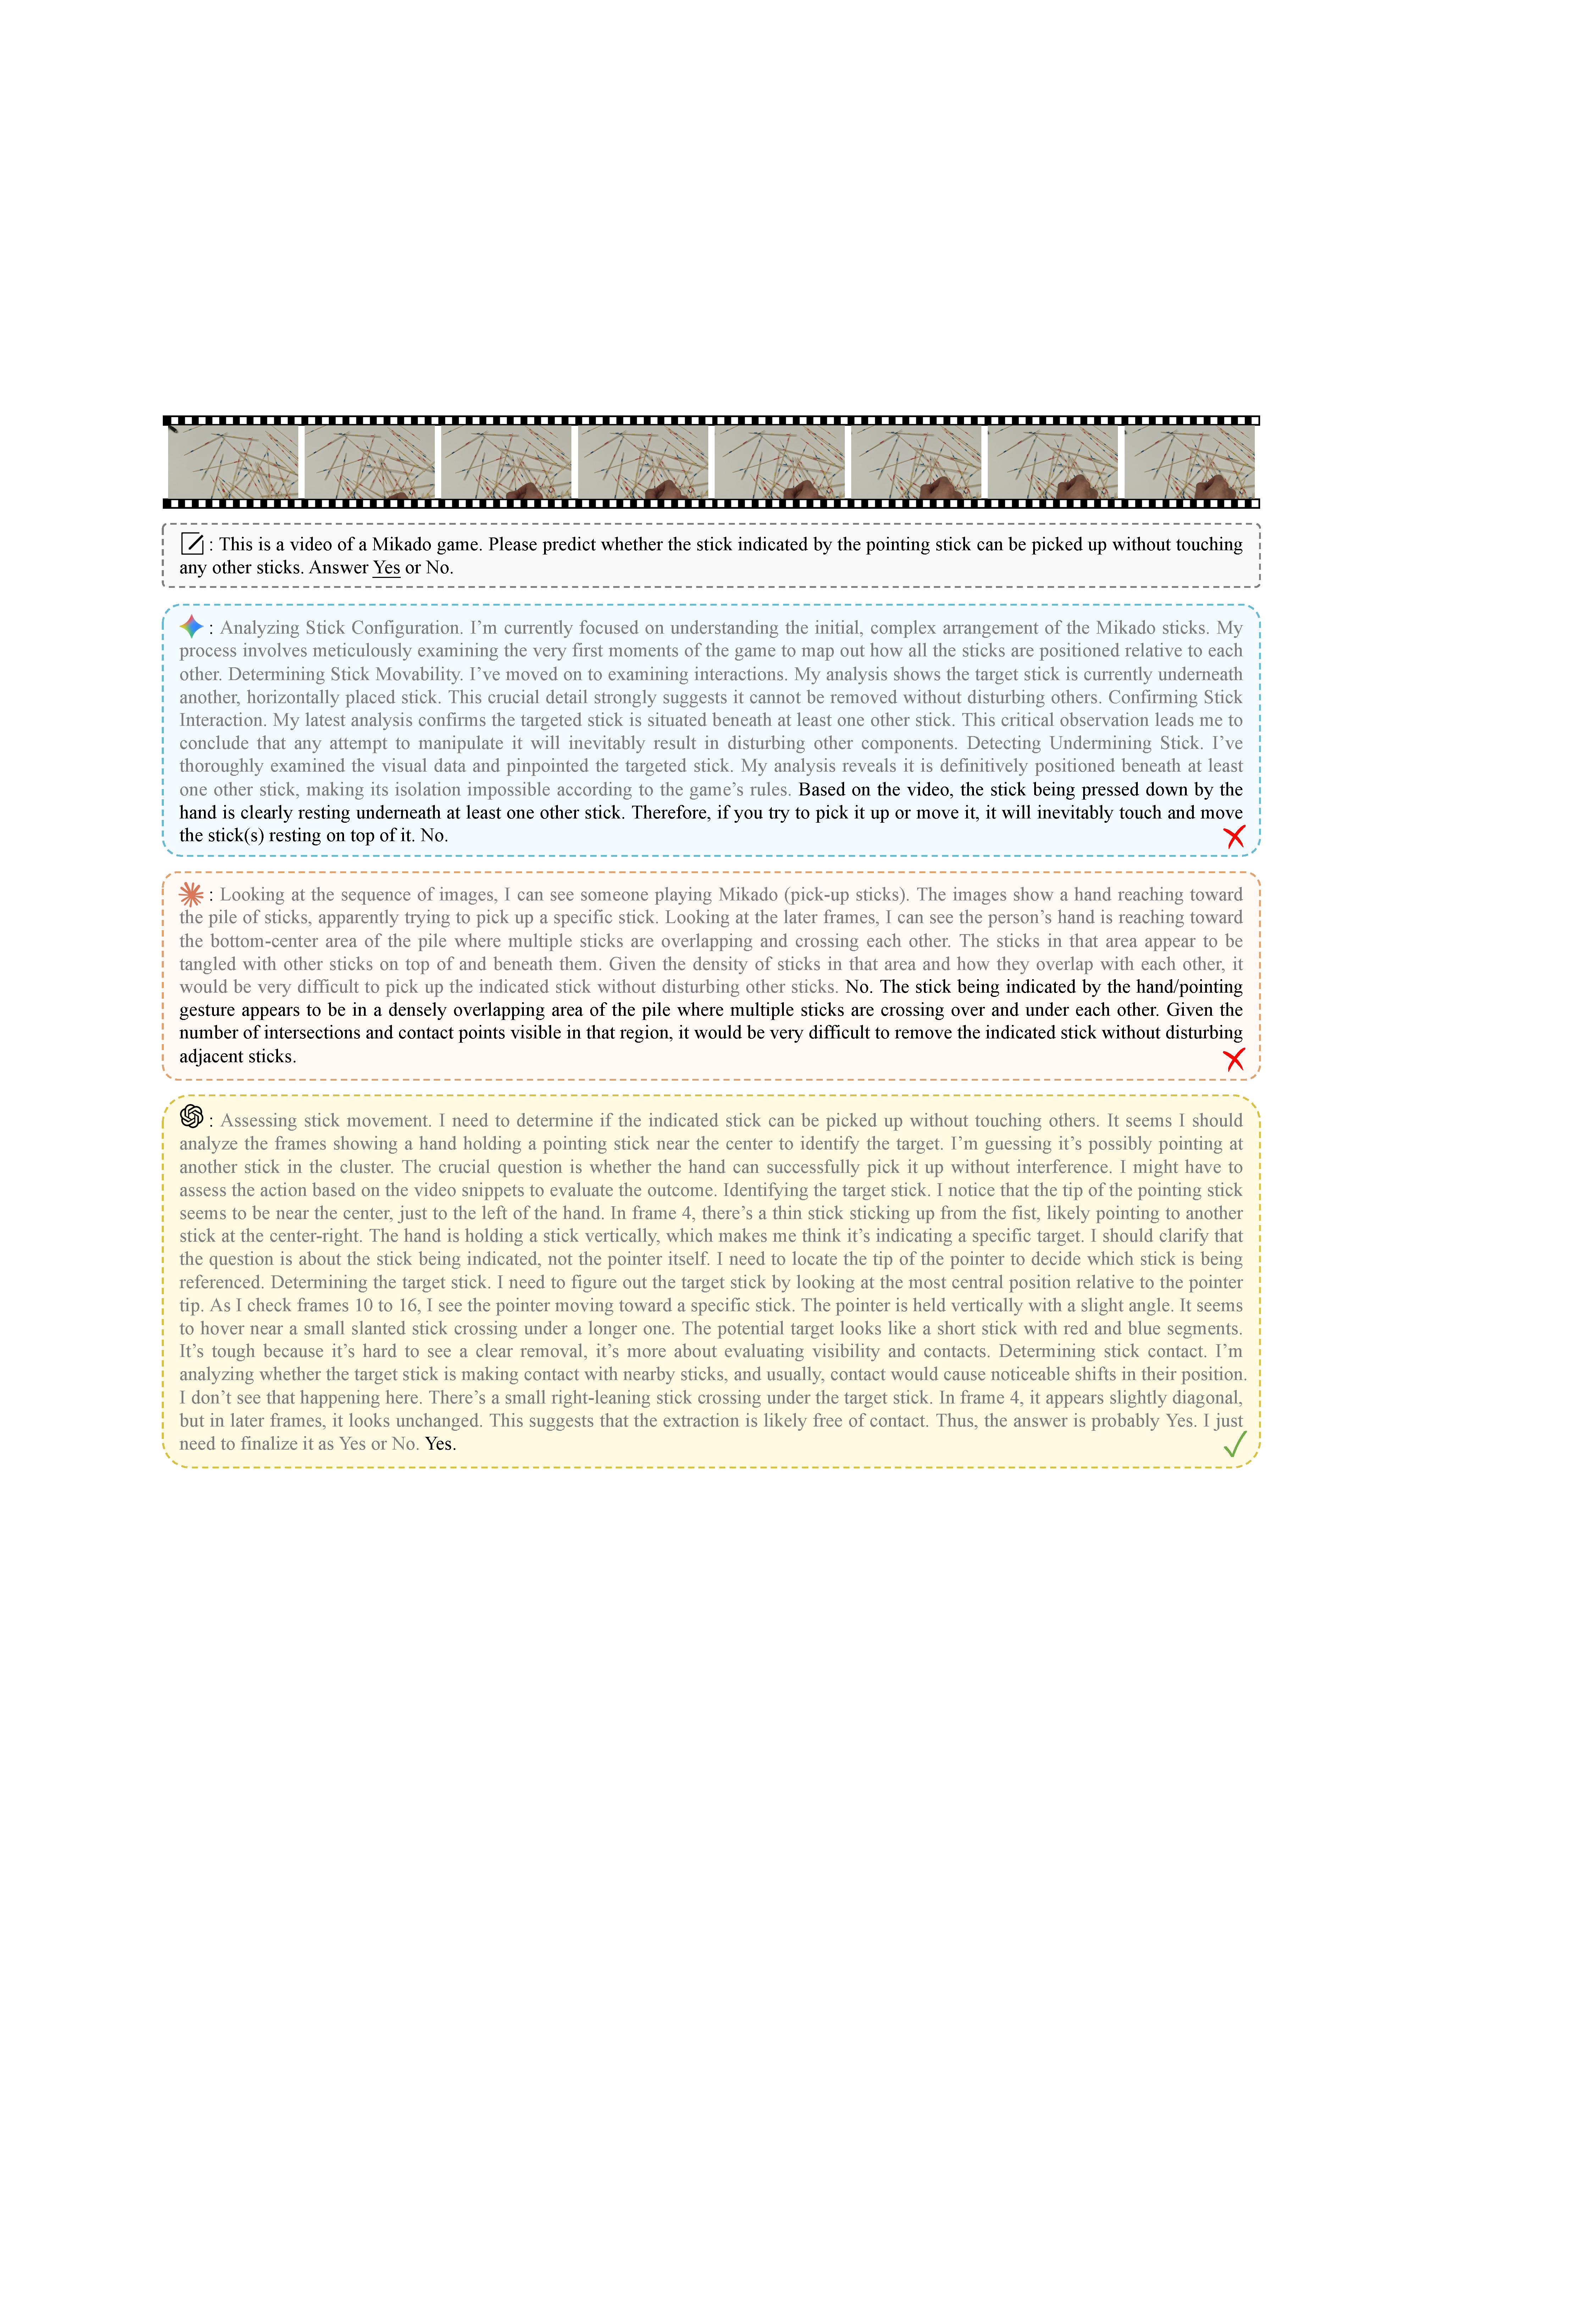
\includegraphics[width=0.95\linewidth]{fig/fig_29.pdf}
  \caption{\textbf{Qualitative visualization for Mikado Dependency.}
  We compare the outputs of GPT-5.4-thinking~\citep{GPT-5}, Gemini-3.1-Pro-Preview~\citep{Gemini}, and Claude-Opus-4.6-thinking~\citep{Claude}.
  Gray text denotes built-in thinking content.}
  \label{fig:29}
\end{figure}

\begin{figure}[p]
  \centering
  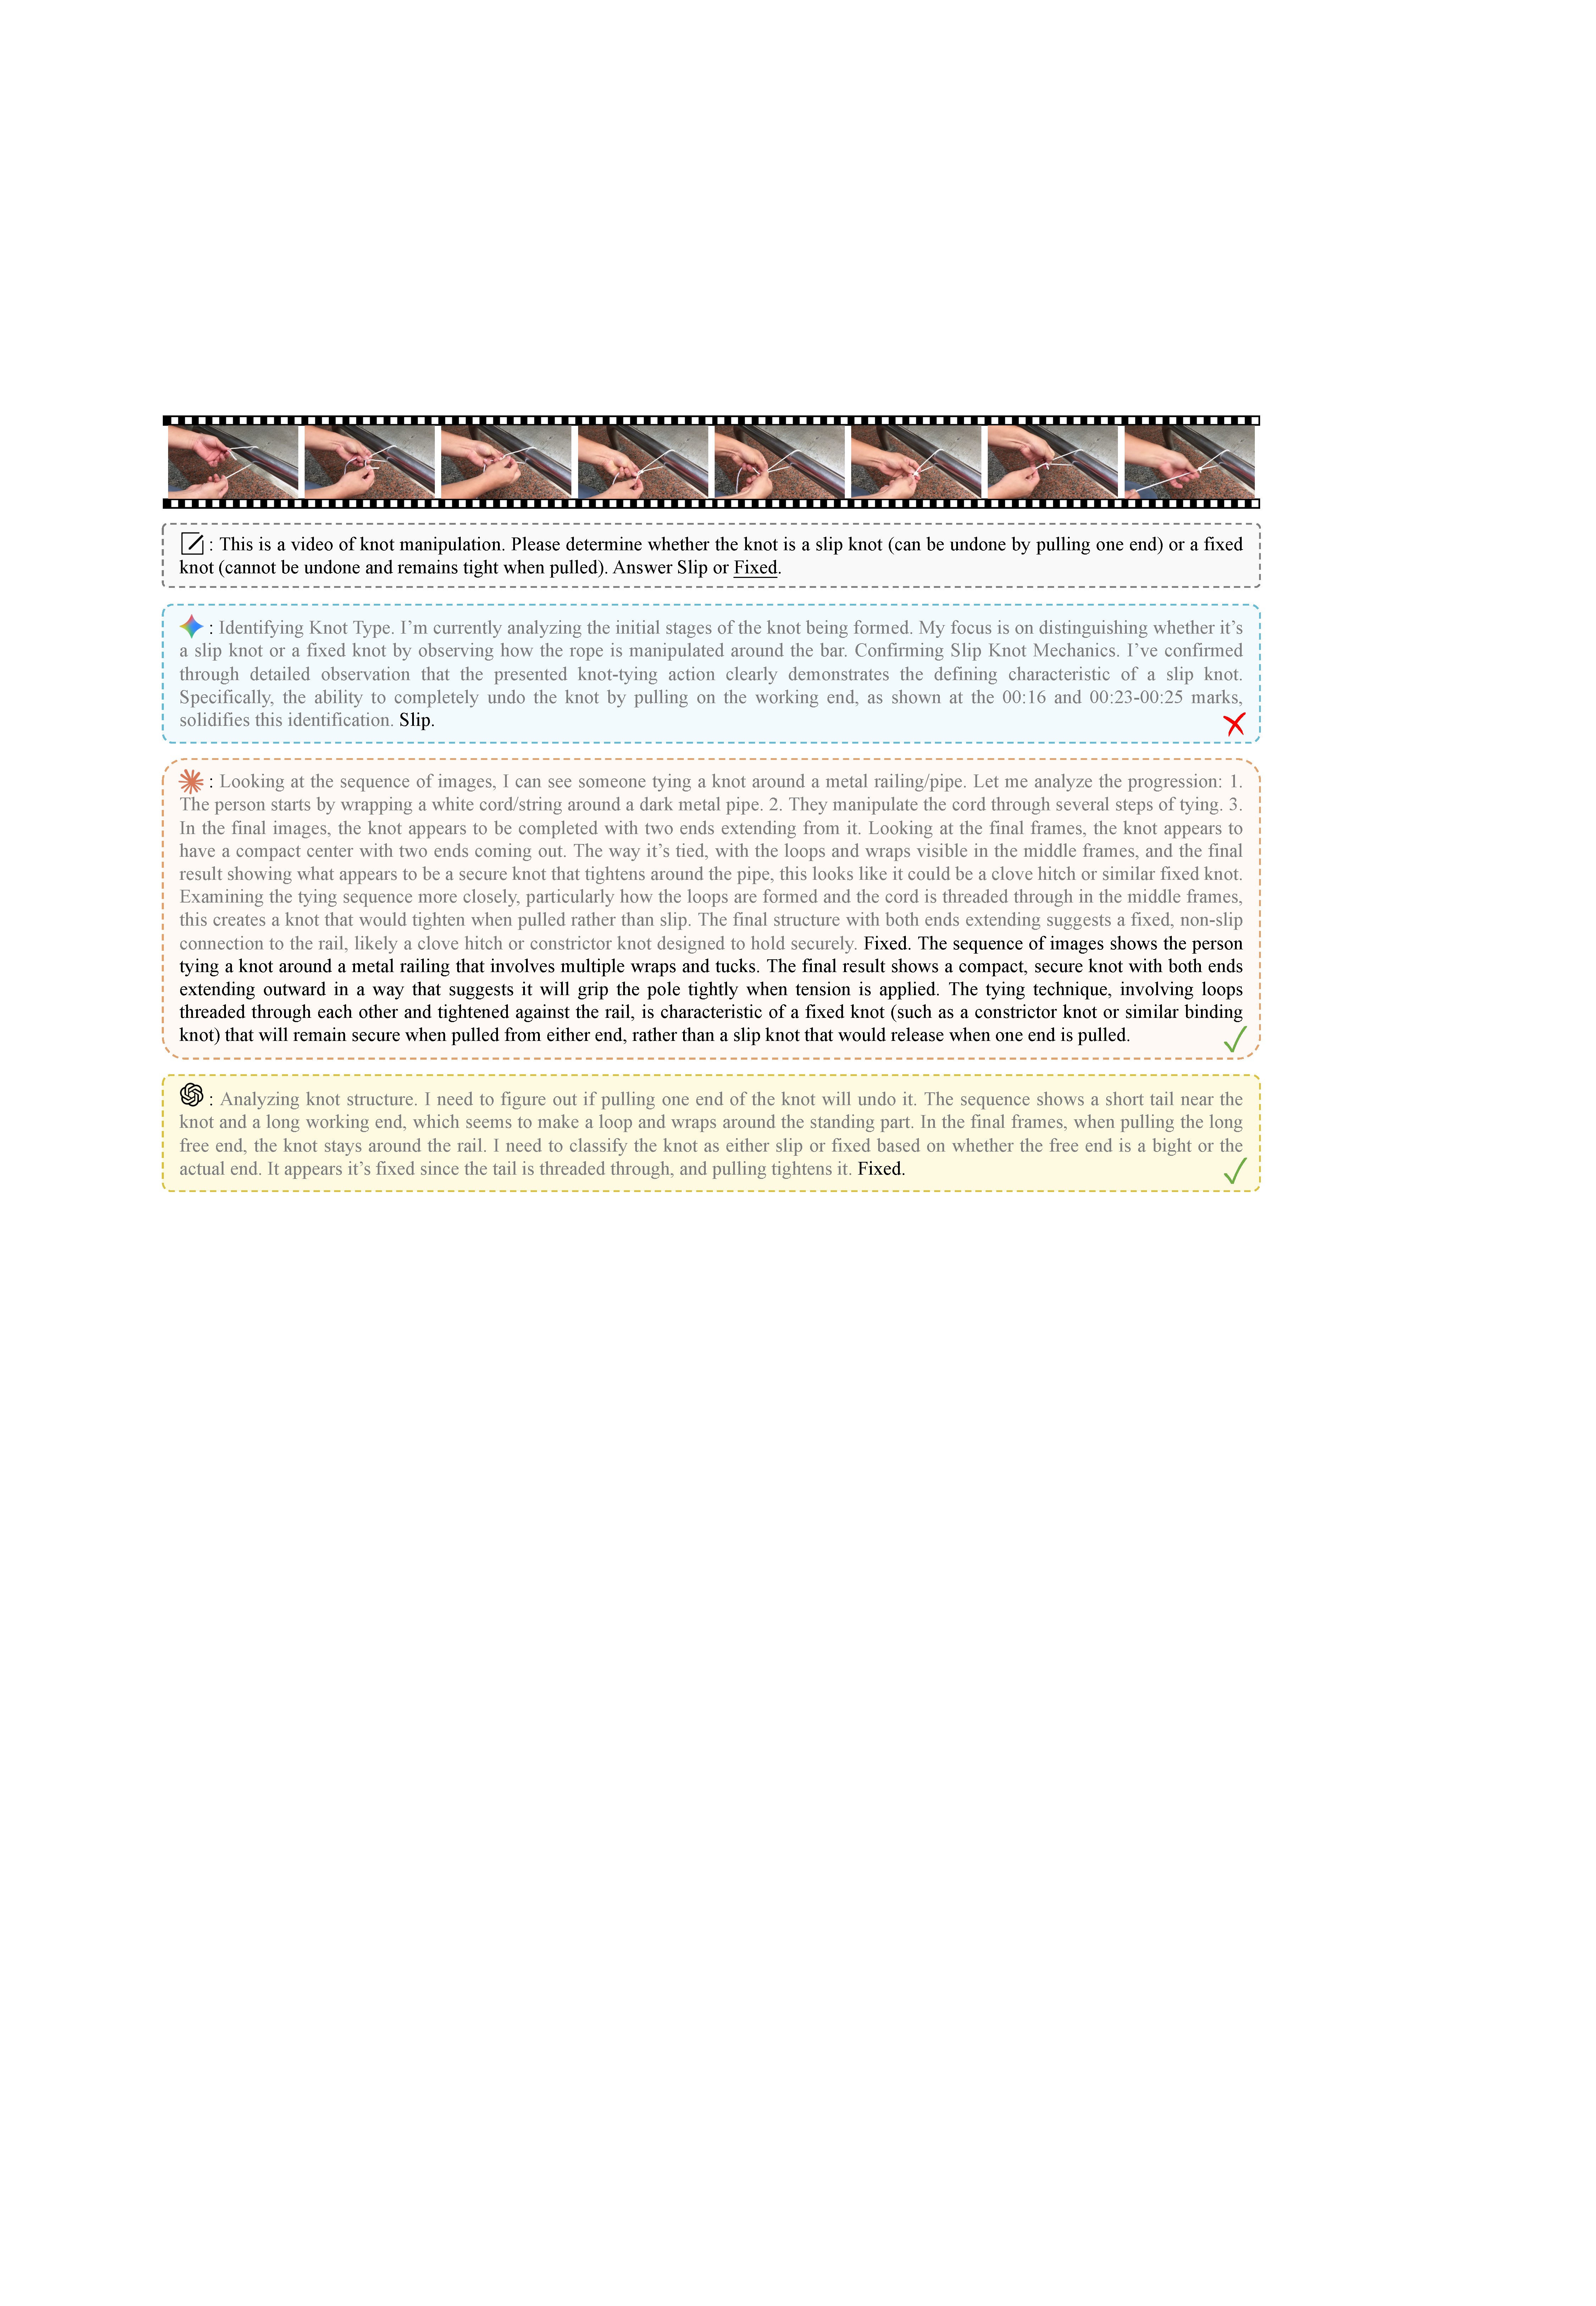
\includegraphics[width=0.95\linewidth]{fig/fig_30.pdf}
  \caption{\textbf{Qualitative visualization for Knot Type.}
  We compare the outputs of GPT-5.4-thinking~\citep{GPT-5}, Gemini-3.1-Pro-Preview~\citep{Gemini}, and Claude-Opus-4.6-thinking~\citep{Claude}.
  Gray text denotes built-in thinking content.}
  \label{fig:30}
\end{figure}


%% ============================================================
%%  Appendix B — tcolorbox Environments Demo (Requirement 6)
%% ============================================================
% \section{Prompt and Analysis Boxes}

% The following boxes demonstrate the tcolorbox environments defined in
% \texttt{colab.sty} for use in appendices.

% \begin{colabinsight}
% The core insight behind our approach is that hierarchical representations
% combined with contrastive pre-training produce features that are both
% discriminative and transferable across tasks.  The multi-scale fusion
% module is the critical component enabling this synergy.
% \end{colabinsight}

% \begin{colabtakeaway}
% When deploying representation learning models, practitioners should:
% \begin{enumerate}[leftmargin=1.5em]
%   \item Pre-train with contrastive objectives on large unlabeled corpora.
%   \item Use hierarchical features instead of single-scale extraction.
%   \item Fine-tune end-to-end with the combined loss for best results.
% \end{enumerate}
% \end{colabtakeaway}

% \begin{colablimitations}
% \begin{itemize}
%   \item The pre-training phase requires 8$\times$A100 GPUs for 72 hours,
%         which may be prohibitive for smaller labs.
%   \item Performance gains diminish on datasets with fewer than 1,000 labeled
%         samples.
%   \item The method has not been tested on modalities beyond vision and language.
% \end{itemize}
% \end{colablimitations}

% \begin{colabprompt}[System Prompt for Evaluation]
% You are an expert evaluator for machine learning research papers. Given the
% following paper excerpt, assess the quality of the experimental methodology
% on a scale of 1--5, considering:

% 1. Reproducibility: Are the experimental details sufficient?
% 2. Baselines: Are the comparisons fair and comprehensive?
% 3. Ablations: Do the ablation studies adequately isolate contributions?
% 4. Statistical rigor: Are error bars or significance tests provided?

% Provide your assessment in JSON format with keys: score, strengths, weaknesses,
% and suggestions.
% \end{colabprompt}

\end{document}
